\documentclass{article}

\usepackage{amsmath} % For writing mathematics (align, split environments etc.)
\usepackage{mathtools}
% \usepackage{amsthm} % For the proof environment
\usepackage{amsfonts} 
\usepackage{geometry}
\usepackage{float}
\usepackage{graphicx}
\usepackage{soul}
\usepackage{indentfirst}
\usepackage{multicol}
\usepackage{tikz}
\usepackage{cancel}

\usetikzlibrary{calc, automata, chains, arrows.meta, math}
\setcounter{MaxMatrixCols}{20}

\usepackage{biblatex}
\addbibresource{bibliography.bib}


\title{A game theoretic model of the behavioural gaming that takes place at the EMS - ED interface}
\author{}
\date{}

\begin{document}
\maketitle

\section{Figures that might be useful}
\begin{figure}[h]
    \centering
    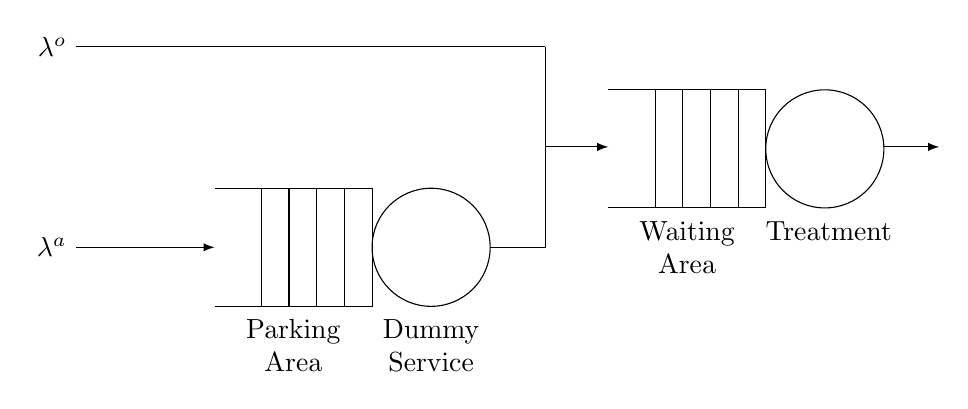
\begin{tikzpicture}[>=latex]
        % the rectangle with vertical rules (Queue 1)
        \draw (0,0) -- ++(2cm,0) -- ++(0,-1.5cm) -- ++(-2cm,0);
        \foreach \i in {1,...,4}
        \draw (2cm-\i*10pt,0) -- +(0,-1.5cm);
        
        % the circle (Queue 1)
        \draw (2.75,-0.75cm) circle [radius=0.75cm];

        % the rectangle with vertical rules (Queue 2)
        \draw (5,1.25) -- ++(2cm,0) -- ++(0,-1.5cm) -- ++(-2cm,0);
        \foreach \i in {1,...,4}
        \draw (7cm-\i*10pt,1.25) -- +(0,-1.5cm);

        % the circle (Queue 2)
        \draw (7.75,0.5) circle [radius=0.75cm];

        % the arrows and labels (Queue 1+2)
        \draw[-] (3.5,-0.75) -- +(20pt,0);
        \draw[<-] (0,-0.75) -- +(-50pt,0) node[left] {\( \lambda^a \)};
        \draw[->] (8.5,0.525) -- +(20pt,0);
        \node[align=center] at (1cm,-2cm) {Parking \\ Area};
        \node[align=center] at (2.75cm,-2cm) {Dummy \\ Service};
        \node[align=center] at (6cm,-0.75cm) {Waiting \\ Area};
        \node[align=center] at (7.8cm,-0.75cm) {Treatment \\ };
        
        \draw (4.2, 1.8) -- +(-169.5pt,0) node[left] {\( \lambda^o \)};
        \draw (4.2, 1.8) -- (4.2, -0.75);
        \draw[->] (4.2, 0.525) -- (5, 0.525);

    \end{tikzpicture}
\end{figure}


\begin{figure}
    \centering
    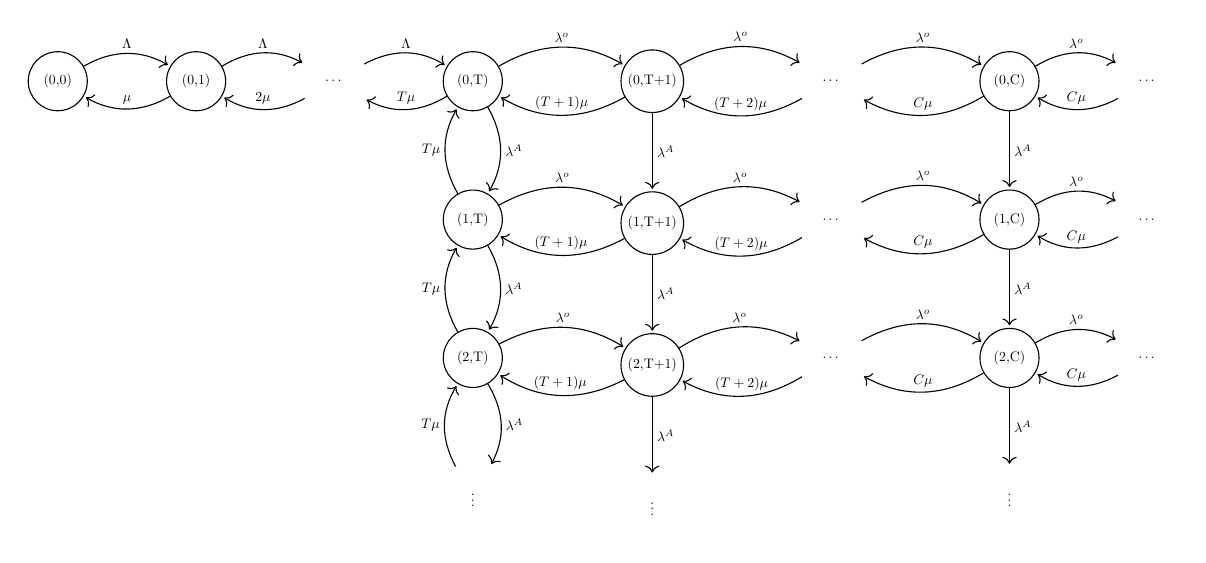
\begin{tikzpicture}[-, node distance = 1cm, auto, every node/.style={scale=0.5}]

        % Variables
        \tikzmath{
            let \altdist = 1.5cm;
            let \minsz = 1.5cm;
        }

        % First Line
        \node[state, minimum size=1.5cm] (zero) {(0,0)};
        \node[state, minimum size=1.5cm,  right=of zero] (one) {(0,1)};
        \node[draw=none, minimum size=1.5cm, right=of one] (two) {\dots};
        \node[state, minimum size=1.5cm, right=of two] (three) {(0,T)};
        \node[state, node distance = \altdist, minimum size=\minsz, right=of three] (four) {(0,T+1)};
        \node[draw=none, node distance = \altdist, minimum size=\minsz, right=of four] (five) {\dots};
        \node[state, node distance = \altdist, minimum size=\minsz, right=of five] (six) {(0,C)};
        \node[draw=none, minimum size=\minsz, right=of six] (seven) {\dots};

        % Second Line
        \node[state, minimum size=\minsz, below=of three] (three_one) {(1,T)};
        \node[state, minimum size=\minsz, below=of four] (four_one) {(1,T+1)};
        \node[draw=none, minimum size=\minsz, below=of five] (five_one) {\dots};
        \node[state, node distance = \altdist, minimum size=\minsz, right=of five_one] (six_one) {(1,C)};
        \node[draw=none, minimum size=\minsz, right=of six_one] (seven_one) {\dots};

        % Third Line
        \node[state, minimum size=\minsz, below=of three_one] (three_two) {(2,T)};
        \node[state, minimum size=\minsz, below=of four_one] (four_two) {(2,T+1)};
        \node[draw=none, minimum size=\minsz, below=of five_one] (five_two) {\dots};
        \node[state, node distance = \altdist, minimum size=\minsz, right=of five_two] (six_two) {(2,C)};
        \node[draw=none, minimum size=\minsz, right=of six_two] (seven_two) {\dots};

        % Fourth line
        \node[draw=none, minimum size=\minsz, below=of three_two] (three_three) {\vdots};
        \node[draw=none, minimum size=\minsz, below=of four_two] (four_three) {\vdots};
        \node[draw=none, minimum size=\minsz, below=of five_two] (five_three) {};
        \node[draw=none, node distance = \altdist, minimum size=\minsz, right=of five_three] (six_three) {\vdots};

        \draw[every loop]
            % First Horizontal Edges
            (zero) edge[bend left] node {\( \Lambda \)} (one)
            (one) edge[bend left] node [above] {\( \mu \)} (zero)
            (one) edge[bend left] node {\( \Lambda \)} (two)
            (two) edge[bend left] node [above] {\( 2 \mu \)} (one)
            (two) edge[bend left] node {\( \Lambda \)} (three)
            (three) edge[bend left] node [above] {\( T \mu \)} (two)
            (three) edge[bend left] node {\( \lambda^o \)} (four)
            (four) edge[bend left] node [above] {\( (T+1) \mu \)} (three)
            (four) edge[bend left] node {\( \lambda^o \)} (five)
            (five) edge[bend left] node [above] {\( (T+2) \mu \)} (four)
            (five) edge[bend left] node {\( \lambda^o \)} (six)
            (six) edge[bend left] node [above] {\( C\mu \)} (five)
            (six) edge[bend left] node {\( \lambda^o \)} (seven)
            (seven) edge[bend left] node [above] {\( C\mu \)} (six)

            % Second Horizontal Edges
            (three_one) edge[bend left] node {\( \lambda^o \)} (four_one)
            (four_one) edge[bend left] node [above] {\( (T+1) \mu \)} (three_one)
            (four_one) edge[bend left] node {\( \lambda^o \)} (five_one)
            (five_one) edge[bend left] node [above] {\( (T+2) \mu \)} (four_one)
            (five_one) edge[bend left] node {\( \lambda^o \)} (six_one)
            (six_one) edge[bend left] node [above] {\( C\mu \)} (five_one)
            (six_one) edge[bend left] node {\( \lambda^o \)} (seven_one)
            (seven_one) edge[bend left] node [above] {\( C\mu \)} (six_one)

            % Third Horizontal Edges
            (three_two) edge[bend left] node {\( \lambda^o \)} (four_two)
            (four_two) edge[bend left] node [above] {\( (T+1) \mu \)} (three_two)
            (four_two) edge[bend left] node {\( \lambda^o \)} (five_two)
            (five_two) edge[bend left] node [above] {\( (T+2) \mu \)} (four_two)
            (five_two) edge[bend left] node {\( \lambda^o \)} (six_two)
            (six_two) edge[bend left] node [above] {\( C\mu \)} (five_two)
            (six_two) edge[bend left] node {\( \lambda^o \)} (seven_two)
            (seven_two) edge[bend left] node [above] {\( C\mu \)} (six_two)

            % First Vertical Edges
            (three) edge[bend left] node {\( \lambda^A \)} (three_one)
            (three_one) edge[bend left] node {\( T \mu \)} (three)
            (three_one) edge[bend left] node {\( \lambda^A \)} (three_two)
            (three_two) edge[bend left] node {\( T\mu \)} (three_one)
            (three_two) edge[bend left] node {\( \lambda^A \)} (three_three)
            (three_three) edge[bend left] node {\( T\mu \)} (three_two)

            % Second Vertical Edges
            (four) edge node {\( \lambda^A \)} (four_one)
            (four_one) edge node {\( \lambda^A \)} (four_two)
            (four_two) edge node {\( \lambda^A \)} (four_three)

            %Third Vertical Edges
            (six) edge node {\( \lambda^A \)} (six_one)
            (six_one) edge node {\( \lambda^A \)} (six_two)
            (six_two) edge node {\( \lambda^A \)} (six_three)
            ;       
    \end{tikzpicture}
    \caption{Markov chains} 
    \label{Markov_2}
\end{figure}



\begin{figure}
    \centering
    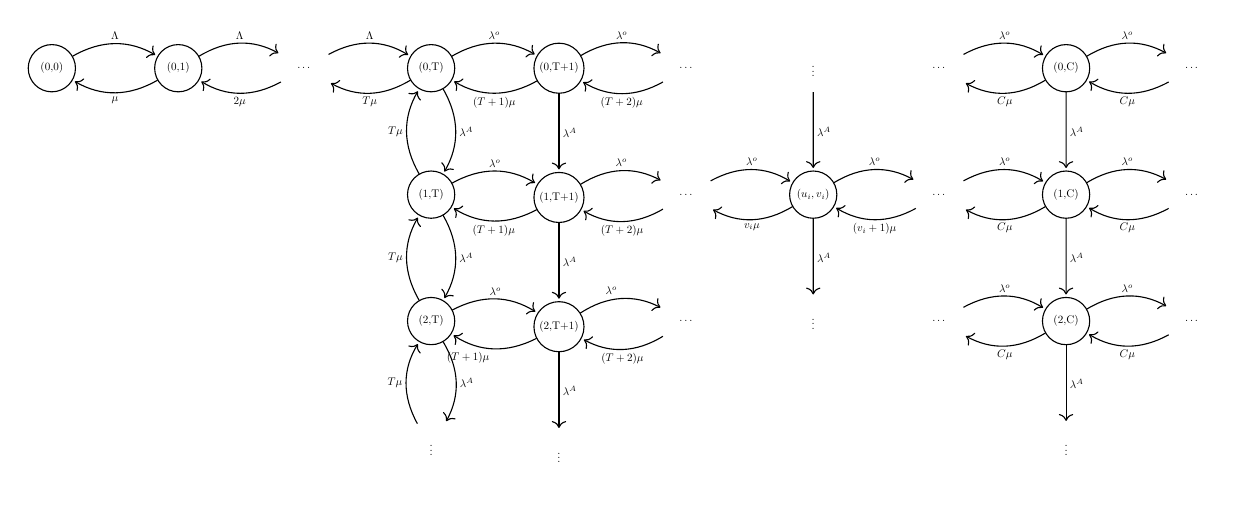
\begin{tikzpicture}[-, node distance = 1cm, auto, every node/.style={scale=0.4}]

        % Variables
        \tikzmath{
            let \altdist = 1cm;
            let \minsz = 1.5cm;
        }

        % First Line
        \node[state, minimum size=1.5cm] (zero) {(0,0)};
        \node[state, minimum size=1.5cm,  right=of zero] (one) {(0,1)};
        \node[draw=none, minimum size=1.5cm, right=of one] (two) {\dots};
        \node[state, minimum size=1.5cm, right=of two] (three) {(0,T)};
        \node[state, node distance = \altdist, minimum size=\minsz, right=of three] (four) {(0,T+1)};
        \node[draw=none, minimum size=\minsz, right=of four] (five) {\dots};
        \node[draw=none, minimum size=\minsz, right=of five] (six) {\vdots};
        \node[draw=none, minimum size=\minsz, right=of six] (seven) {\dots};
        \node[state, minimum size=\minsz, right=of seven] (eight) {(0,C)};
        \node[draw=none, minimum size=\minsz, right=of eight] (nine) {\dots};


        % Second Line
        \node[state, minimum size=\minsz, below=of three] (three_one) {(1,T)};
        \node[state, minimum size=\minsz, below=of four] (four_one) {(1,T+1)};
        \node[draw=none, minimum size=\minsz, below=of five] (five_one) {\dots};
        \node[state, node distance = \altdist, minimum size=\minsz, right=of five_one] (six_one) {\( (u_i, v_i) \)};
        \node[draw=none, minimum size=\minsz, right=of six_one] (seven_one) {\dots};
        \node[state, node distance = \altdist, minimum size=\minsz, right=of seven_one] (eight_one) {(1,C)};
        \node[draw=none, minimum size=\minsz, right=of eight_one] (nine_one) {\dots};
        

        % Third Line
        \node[state, minimum size=\minsz, below=of three_one] (three_two) {(2,T)};
        \node[state, minimum size=\minsz, below=of four_one] (four_two) {(2,T+1)};
        \node[draw=none, minimum size=\minsz, below=of five_one] (five_two) {\dots};
        \node[draw=none, node distance = \altdist, minimum size=\minsz, right=of five_two] (six_two) {\vdots};
        \node[draw=none, minimum size=\minsz, right=of six_two] (seven_two) {\dots};
        \node[state, node distance = \altdist, minimum size=\minsz, right=of seven_two] (eight_two) {(2,C)};
        \node[draw=none, minimum size=\minsz, right=of eight_two] (nine_two) {\dots};

        % Fourth line
        \node[draw=none, minimum size=\minsz, below=of three_two] (three_three) {\vdots};
        \node[draw=none, minimum size=\minsz, below=of four_two] (four_three) {\vdots};
        \node[draw=none, minimum size=\minsz, below=of five_two] (five_three) {};
        \node[draw=none, node distance = \altdist, minimum size=\minsz, right=of five_three] (six_three) {};
        \node[draw=none, node distance = \altdist, minimum size=\minsz, below=of eight_two] (eight_three) {\vdots};


        \draw[every loop]
            % First Horizontal Edges
            (zero) edge[bend left] node {\( \Lambda \)} (one)
            (one) edge[bend left] node {\( \mu \)} (zero)
            (one) edge[bend left] node {\( \Lambda \)} (two)
            (two) edge[bend left] node {\( 2 \mu \)} (one)
            (two) edge[bend left] node {\( \Lambda \)} (three)
            (three) edge[bend left] node {\( T \mu \)} (two)
            (three) edge[bend left] node {\( \lambda^o \)} (four)
            (four) edge[bend left] node {\( (T+1) \mu \)} (three)
            (four) edge[bend left] node {\( \lambda^o \)} (five)
            (five) edge[bend left] node {\( (T+2) \mu \)} (four)
            % (five) edge[bend left] node {\( \lambda^o \)} (six)
            % (six) edge[bend left] node [above] {\( C\mu \)} (five)
            % (six) edge[bend left] node {\( \lambda^o \)} (seven)
            % (seven) edge[bend left] node [above] {\( C\mu \)} (six)
            (seven) edge[bend left] node {\( \lambda^o \)} (eight)
            (eight) edge[bend left] node {\( C\mu \)} (seven)
            (eight) edge[bend left] node {\( \lambda^o \)} (nine)
            (nine) edge[bend left] node {\( C\mu \)} (eight)

            % Second Horizontal Edges
            (three_one) edge[bend left] node {\(\lambda^o\)} (four_one)
            (four_one) edge[bend left] node {\( (T+1) \mu \)} (three_one)
            (four_one) edge[bend left] node {\( \lambda^o \)} (five_one)
            (five_one) edge[bend left] node {\( (T+2) \mu \)} (four_one)
            (five_one) edge[bend left] node {\( \lambda^o \)} (six_one)
            (six_one) edge[bend left] node {\( v_i\mu \)} (five_one)
            (six_one) edge[bend left] node {\( \lambda^o \)} (seven_one)
            (seven_one) edge[bend left] node {\( (v_i+1)\mu \)} (six_one)
            (seven_one) edge[bend left] node {\( \lambda^o \)} (eight_one)
            (eight_one) edge[bend left] node {\( C\mu \)} (seven_one)
            (eight_one) edge[bend left] node {\( \lambda^o \)} (nine_one)
            (nine_one) edge[bend left] node {\( C\mu \)} (eight_one)

            % Third Horizontal Edges
            (three_two) edge[bend left] node {\( \lambda^o \)} (four_two)
            (four_two) edge[bend left] node {\( (T+1) \mu \)} (three_two)
            (four_two) edge[bend left] node {\( \lambda^o \)} (five_two)
            (five_two) edge[bend left] node {\( (T+2) \mu \)} (four_two)
            % (five_two) edge[bend left] node {\( \lambda^o \)} (six_two)
            % (six_two) edge[bend left] node [above] {\( C\mu \)} (five_two)
            % (six_two) edge[bend left] node {\( \lambda^o \)} (seven_two)
            % (seven_two) edge[bend left] node [above] {\( C\mu \)} (six_two)
            (seven_two) edge[bend left] node {\( \lambda^o \)} (eight_two)
            (eight_two) edge[bend left] node {\( C\mu \)} (seven_two)
            (eight_two) edge[bend left] node {\( \lambda^o \)} (nine_two)
            (nine_two) edge[bend left] node {\( C\mu \)} (eight_two)

            % First Vertical Edges
            (three) edge[bend left] node {\( \lambda^A \)} (three_one)
            (three_one) edge[bend left] node {\( T \mu \)} (three)
            (three_one) edge[bend left] node {\( \lambda^A \)} (three_two)
            (three_two) edge[bend left] node {\( T\mu \)} (three_one)
            (three_two) edge[bend left] node {\( \lambda^A \)} (three_three)
            (three_three) edge[bend left] node {\( T\mu \)} (three_two)

            % Second Vertical Edges
            (four) edge node {\( \lambda^A \)} (four_one)
            (four_one) edge node {\( \lambda^A \)} (four_two)
            (four_two) edge node {\( \lambda^A \)} (four_three)

            % Third Vertical Edges
            (six) edge node {\( \lambda^A \)} (six_one)
            (six_one) edge node {\( \lambda^A \)} (six_two)
            % (six_two) edge node {\( \lambda^A \)} (six_three)

            % Fourth Vertical Edges
            (eight) edge node {\( \lambda^A \)} (eight_one)
            (eight_one) edge node {\( \lambda^A \)} (eight_two)
            (eight_two) edge node {\( \lambda^A \)} (eight_three)
            ;       
    \end{tikzpicture}
    \caption{Markov chains} 
    \label{Markov_3}
\end{figure}


\begin{figure}
    \centering
    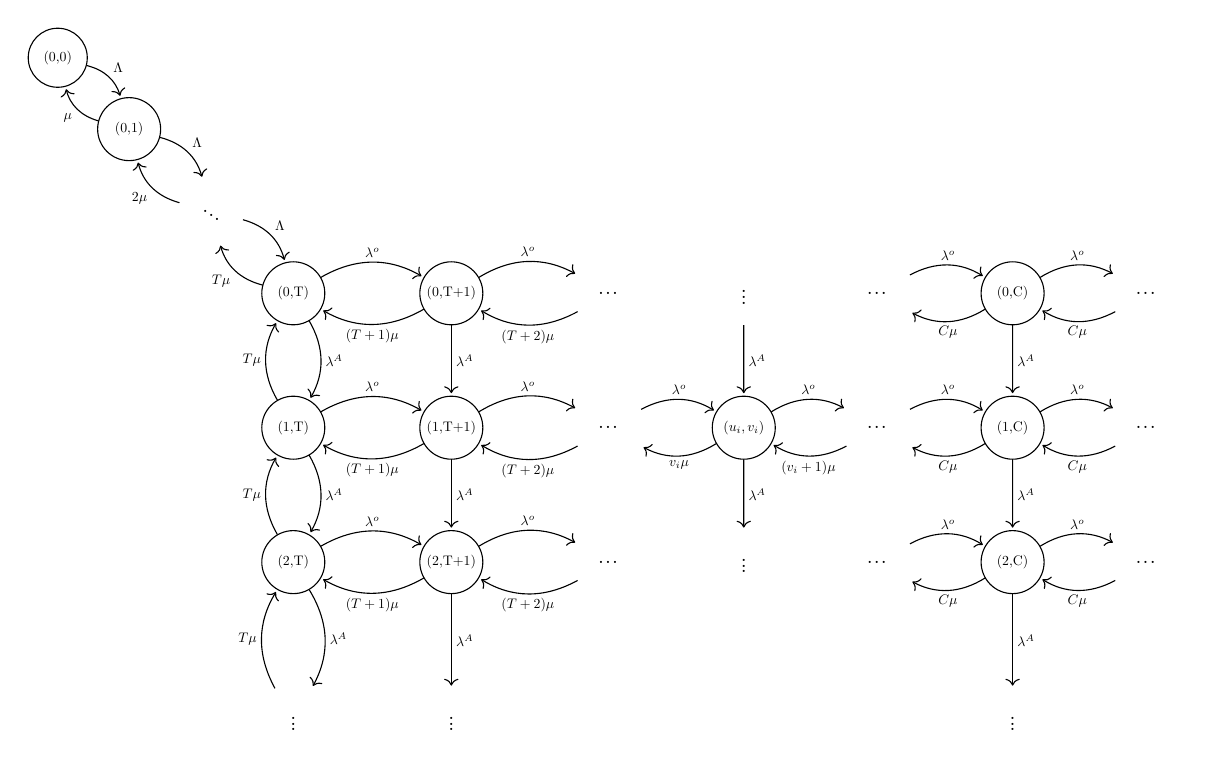
\begin{tikzpicture}[-, node distance = 0.9cm, auto, every node/.style={scale=0.5}]

        % Variables
        \tikzmath{
            let \initdist = 0.5cm;
            let \altdist = 1.2cm;
            let \minsz = 1.6cm;
            let \leftOne = -0.8;
            let \rightOne = 2.2;
            let \upOne = 0.8;
            let \downOne = -2.2;
            let \leftTwo = 2.25;
            let \rightTwo = 14.2;
            let \upTwo = -2.35;
            let \downTwo = -8.8;
        }

        % % Rectangle for S1
        % \draw[ultra thin, dashed] (\leftOne, \downOne) -- (\leftOne, \upOne);
        % \draw[ultra thin, dashed] (\leftOne, \upOne) -- (\rightOne, \upOne);
        % \draw[ultra thin, dashed] (\rightOne, \upOne) -- node {\Huge{\( \quad S_1 \)}}(\rightOne, \downOne);
        % \draw[ultra thin, dashed] (\rightOne, \downOne) -- (\leftOne, \downOne);

        % % Rectangle for S2
        % \draw[ultra thin, dashed] (\leftTwo, \downTwo) -- node {\Huge{\( S_2 \quad \)}}(\leftTwo, \upTwo);
        % \draw[ultra thin, dashed] (\leftTwo, \upTwo) -- (\rightTwo, \upTwo);
        % \draw[ultra thin, dashed] (\rightTwo, \upTwo) -- (\rightTwo, \downTwo);
        % \draw[ultra thin, dashed] (\rightTwo, \downTwo) -- (\leftTwo, \downTwo);

        % First Line
        \node[state, minimum size=1.5cm] (zero) {(0,0)};
        \node[state, node distance = \initdist, minimum size=\minsz, below right=of zero] (one) {(0,1)};
        \node[draw=none, node distance = \initdist, minimum size=\minsz, below right=of one] (two) {\textbf{\( \ddots \)}};
        \node[state, node distance = \initdist, minimum size=\minsz, below right=of two] (three) {(0,T)};
        \node[state, node distance = \altdist, minimum size=\minsz, right=of three] (four) {(0,T+1)};
        \node[draw=none, node distance = \altdist, minimum size=\minsz, right=of four] (five) {\textbf{\dots}};
        \node[draw=none, minimum size=\minsz, right=of five] (six) {\textbf{\vdots}};
        \node[draw=none, minimum size=\minsz, right=of six] (seven) {\textbf{\dots}};
        \node[state, minimum size=\minsz, right=of seven] (eight) {(0,C)};
        \node[draw=none, minimum size=\minsz, right=of eight] (nine) {\textbf{\dots}};


        % Second Line
        \node[state, minimum size=\minsz, below=of three] (three_one) {(1,T)};
        \node[state, minimum size=\minsz, below=of four] (four_one) {(1,T+1)};
        \node[draw=none, minimum size=\minsz, below=of five] (five_one) {\textbf{\dots}};
        \node[state, minimum size=\minsz, right=of five_one] (six_one) {\( (u_i, v_i) \)};
        \node[draw=none, minimum size=\minsz, right=of six_one] (seven_one) {\textbf{\dots}};
        \node[state, minimum size=\minsz, right=of seven_one] (eight_one) {(1,C)};
        \node[draw=none, minimum size=\minsz, right=of eight_one] (nine_one) {\textbf{\dots}};
        

        % Third Line
        \node[state, minimum size=\minsz, below=of three_one] (three_two) {(2,T)};
        \node[state, minimum size=\minsz, below=of four_one] (four_two) {(2,T+1)};
        \node[draw=none, minimum size=\minsz, below=of five_one] (five_two) {\textbf{\dots}};
        \node[draw=none, minimum size=\minsz, right=of five_two] (six_two) {\textbf{\vdots}};
        \node[draw=none, minimum size=\minsz, right=of six_two] (seven_two) {\textbf{\dots}};
        \node[state, minimum size=\minsz, right=of seven_two] (eight_two) {(2,C)};
        \node[draw=none, minimum size=\minsz, right=of eight_two] (nine_two) {\textbf{\dots}};

        % Fourth line
        \node[draw=none, node distance = \altdist, minimum size=\minsz, below=of three_two] (three_three) {\textbf{\vdots}};
        \node[draw=none, node distance = \altdist, minimum size=\minsz, below=of four_two] (four_three) {\textbf{\vdots}};
        \node[draw=none, node distance = \altdist, minimum size=\minsz, below=of five_two] (five_three) {};
        \node[draw=none, node distance = \altdist, minimum size=\minsz, below=of six_two] (six_three) {};
        \node[draw=none, node distance = \altdist, minimum size=\minsz, below=of eight_two] (eight_three) {\textbf{\vdots}};


        \draw[every loop]
            % First Horizontal Edges
            (zero) edge[bend left] node {\( \Lambda \)} (one)
            (one) edge[bend left] node {\( \mu \)} (zero)
            (one) edge[bend left] node {\( \Lambda \)} (two)
            (two) edge[bend left] node {\( 2 \mu \)} (one)
            (two) edge[bend left] node {\( \Lambda \)} (three)
            (three) edge[bend left] node {\( T \mu \)} (two)
            (three) edge[bend left] node {\( \lambda^o \)} (four)
            (four) edge[bend left] node {\( (T+1) \mu \)} (three)
            (four) edge[bend left] node {\( \lambda^o \)} (five)
            (five) edge[bend left] node {\( (T+2) \mu \)} (four)
            % (five) edge[bend left] node {\( \lambda^o \)} (six)
            % (six) edge[bend left] node [above] {\( C\mu \)} (five)
            % (six) edge[bend left] node {\( \lambda^o \)} (seven)
            % (seven) edge[bend left] node [above] {\( C\mu \)} (six)
            (seven) edge[bend left] node {\( \lambda^o \)} (eight)
            (eight) edge[bend left] node {\( C\mu \)} (seven)
            (eight) edge[bend left] node {\( \lambda^o \)} (nine)
            (nine) edge[bend left] node {\( C\mu \)} (eight)

            % Second Horizontal Edges
            (three_one) edge[bend left] node {\( \lambda^o \)} (four_one)
            (four_one) edge[bend left] node {\( (T+1) \mu \)} (three_one)
            (four_one) edge[bend left] node {\( \lambda^o \)} (five_one)
            (five_one) edge[bend left] node {\( (T+2) \mu \)} (four_one)
            (five_one) edge[bend left] node {\( \lambda^o \)} (six_one)
            (six_one) edge[bend left] node {\( v_i\mu \)} (five_one)
            (six_one) edge[bend left] node {\( \lambda^o \)} (seven_one)
            (seven_one) edge[bend left] node {\( (v_i+1)\mu \)} (six_one)
            (seven_one) edge[bend left] node {\( \lambda^o \)} (eight_one)
            (eight_one) edge[bend left] node {\( C\mu \)} (seven_one)
            (eight_one) edge[bend left] node {\( \lambda^o \)} (nine_one)
            (nine_one) edge[bend left] node {\( C\mu \)} (eight_one)

            % Third Horizontal Edges
            (three_two) edge[bend left] node {\( \lambda^o \)} (four_two)
            (four_two) edge[bend left] node [below] {\( (T+1) \mu \)} (three_two)
            (four_two) edge[bend left] node {\( \lambda^o \)} (five_two)
            (five_two) edge[bend left] node {\( (T+2) \mu \)} (four_two)
            % (five_two) edge[bend left] node {\( \lambda^o \)} (six_two)
            % (six_two) edge[bend left] node [above] {\( C\mu \)} (five_two)
            % (six_two) edge[bend left] node {\( \lambda^o \)} (seven_two)
            % (seven_two) edge[bend left] node [above] {\( C\mu \)} (six_two)
            (seven_two) edge[bend left] node {\( \lambda^o \)} (eight_two)
            (eight_two) edge[bend left] node {\( C\mu \)} (seven_two)
            (eight_two) edge[bend left] node {\( \lambda^o \)} (nine_two)
            (nine_two) edge[bend left] node {\( C\mu \)} (eight_two)

            % First Vertical Edges
            (three) edge[bend left] node {\( \lambda^A \)} (three_one)
            (three_one) edge[bend left] node {\( T \mu \)} (three)
            (three_one) edge[bend left] node {\( \lambda^A \)} (three_two)
            (three_two) edge[bend left] node {\( T\mu \)} (three_one)
            (three_two) edge[bend left] node {\( \lambda^A \)} (three_three)
            (three_three) edge[bend left] node {\( T\mu \)} (three_two)

            % Second Vertical Edges
            (four) edge node {\( \lambda^A \)} (four_one)
            (four_one) edge node {\( \lambda^A \)} (four_two)
            (four_two) edge node {\( \lambda^A \)} (four_three)

            % Third Vertical Edges
            (six) edge node {\( \lambda^A \)} (six_one)
            (six_one) edge node {\( \lambda^A \)} (six_two)
            % (six_two) edge node {\( \lambda^A \)} (six_three)

            % Fourth Vertical Edges
            (eight) edge node {\( \lambda^A \)} (eight_one)
            (eight_one) edge node {\( \lambda^A \)} (eight_two)
            (eight_two) edge node {\( \lambda^A \)} (eight_three)
            ;       
    \end{tikzpicture}
    \caption{Markov chains} 
    \label{Markov_4}
\end{figure}




\begin{figure}
    \centering
    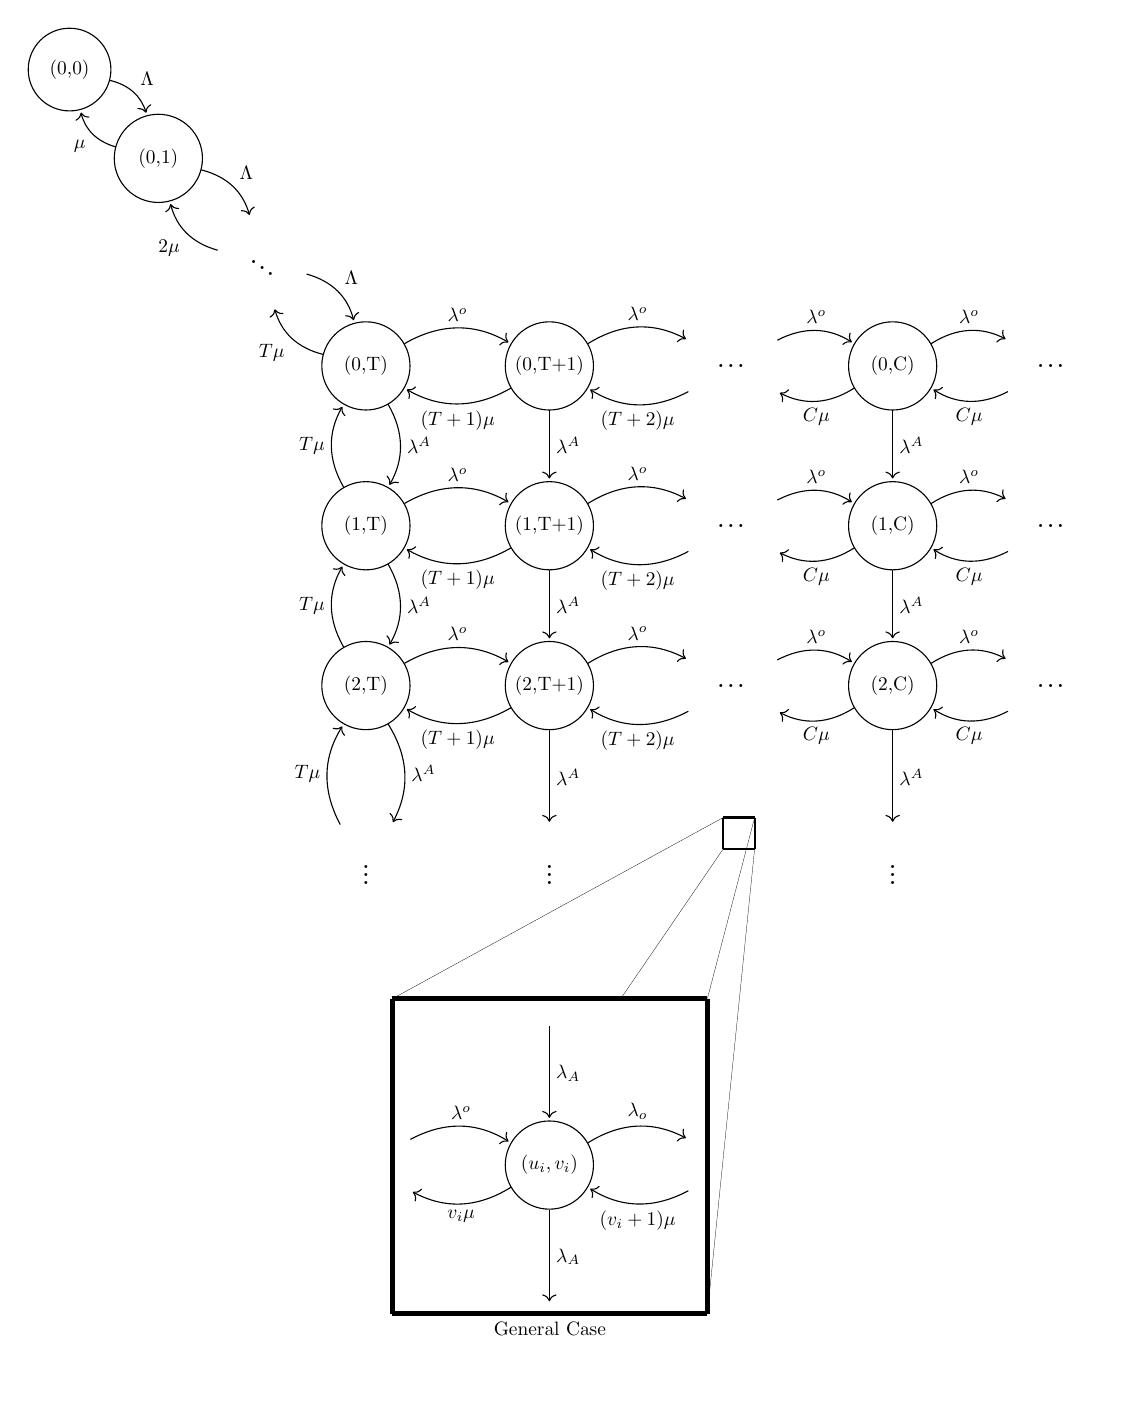
\begin{tikzpicture}[-, node distance = 0.9cm, auto, every node/.style={scale=0.7}]

        % Markov chain variables
        \tikzmath{
            let \initdist = 0.5cm;
            let \altdist = 1.2cm;
            let \minsz = 1.6cm;
        }

        % S_1 and S_2 rectangles
        \tikzmath{
            let \leftOne = -0.8;
            let \rightOne = 2.7;
            let \upOne = 0.8;
            let \downOne = -2.7;
            let \leftTwo = 2.8;
            let \rightTwo = 13;
            let \upTwo = -2.95;
            let \downTwo = -16.4;
        }

        % General case variables
        \tikzmath{
            let \GCsmallx = 8.3;
            let \GCsmally = -9.5;
            let \GCbigx = 4.1;
            let \GCbigy = -11.8;
        }

        % % Rectangle for S1
        % \draw[ultra thin, dashed] (\leftOne, \downOne) -- (\leftOne, \upOne);
        % \draw[ultra thin, dashed] (\leftOne, \upOne) -- (\rightOne, \upOne);
        % \draw[ultra thin, dashed] (\rightOne, \upOne) -- node {\Huge{\( \quad S_1 \)}}(\rightOne, \downOne);
        % \draw[ultra thin, dashed] (\rightOne, \downOne) -- (\leftOne, \downOne);

        % % Rectangle for S2
        % \draw[ultra thin, dashed] (\leftTwo, \downTwo) -- node {\Huge{\( S_2 \quad \)}}(\leftTwo, \upTwo);
        % \draw[ultra thin, dashed] (\leftTwo, \upTwo) -- (\rightTwo, \upTwo);
        % \draw[ultra thin, dashed] (\rightTwo, \upTwo) -- (\rightTwo, \downTwo);
        % \draw[ultra thin, dashed] (\rightTwo, \downTwo) -- (\leftTwo, \downTwo);

        % Small square of general case
        \draw [thick] (\GCsmallx, \GCsmally) -- node {} (\GCsmallx + 0.4, \GCsmally);
        \draw [thick] (\GCsmallx + 0.4, \GCsmally) -- node {} (\GCsmallx + 0.4, \GCsmally - 0.4);
        \draw [thick] (\GCsmallx + 0.4, \GCsmally - 0.4) -- node {} (\GCsmallx, \GCsmally - 0.4);
        \draw [thick] (\GCsmallx, \GCsmally - 0.4) -- node {} (\GCsmallx, \GCsmally);


        % Dashed lines to from small square to big one 
        \draw [ultra thin] (\GCsmallx, \GCsmally) -- node {} (\GCbigx, \GCbigy);
        \draw [ultra thin] (\GCsmallx + 0.4, \GCsmally) -- node {} (\GCbigx + 4, \GCbigy);
        \draw [ultra thin] (\GCsmallx, \GCsmally - 0.4) -- node {} (7, \GCbigy);
        \draw [ultra thin] (\GCsmallx + 0.4, \GCsmally - 0.4) -- node {} (\GCbigx + 4, \GCbigy - 4);
        
        % Big Square of general case
        \draw [ultra thick] (\GCbigx, \GCbigy) -- node {} (\GCbigx + 4, \GCbigy);
        \draw [ultra thick] (\GCbigx + 4, \GCbigy) -- node {} (\GCbigx + 4, \GCbigy - 4);
        \draw [ultra thick] (\GCbigx + 4, \GCbigy - 4) -- node {General Case} (\GCbigx, \GCbigy - 4);
        \draw [ultra thick] (\GCbigx, \GCbigy - 4) -- node {} (\GCbigx, \GCbigy);

        % First Line
        \node[state, minimum size=1.5cm] (zero) {(0,0)};
        \node[state, node distance = \initdist, minimum size=\minsz, below right=of zero] (one) {(0,1)};
        \node[draw=none, node distance = \initdist, minimum size=\minsz, below right=of one] (two) {\textbf{\( \ddots \)}};
        \node[state, node distance = \initdist, minimum size=\minsz, below right=of two] (three) {(0,T)};
        \node[state, node distance = \altdist, minimum size=\minsz, right=of three] (four) {(0,T+1)};
        \node[draw=none, node distance = \altdist, minimum size=\minsz, right=of four] (five) {\textbf{\dots}};
        \node[state, minimum size=\minsz, right=of five] (six) {(0,C)};
        \node[draw=none, minimum size=\minsz, right=of six] (seven) {\textbf{\dots}};

        % Second Line
        \node[state, minimum size=\minsz, below=of three] (three_one) {(1,T)};
        \node[state, minimum size=\minsz, below=of four] (four_one) {(1,T+1)};
        \node[draw=none, minimum size=\minsz, below=of five] (five_one) {\textbf{\dots}};
        \node[state, minimum size=\minsz, right=of five_one] (six_one) {(1,C)};
        \node[draw=none, minimum size=\minsz, right=of six_one] (seven_one) {\textbf{\dots}};
        
        % Third Line
        \node[state, minimum size=\minsz, below=of three_one] (three_two) {(2,T)};
        \node[state, minimum size=\minsz, below=of four_one] (four_two) {(2,T+1)};
        \node[draw=none, minimum size=\minsz, below=of five_one] (five_two) {\textbf{\dots}};
        \node[state, minimum size=\minsz, right=of five_two] (six_two) {(2,C)};
        \node[draw=none, minimum size=\minsz, right=of six_two] (seven_two) {\textbf{\dots}};

        % Fourth line
        \node[draw=none, node distance = \altdist, minimum size=\minsz, below=of three_two] (three_three) {\textbf{\vdots}};
        \node[draw=none, node distance = \altdist, minimum size=\minsz, below=of four_two] (four_three) {\textbf{\vdots}};
        \node[draw=none, node distance = 2cm, minimum size=\minsz, below=of five_two] (five_three) {};
        \node[draw=none, node distance = \altdist, minimum size=\minsz, below=of six_two] (six_three) {\textbf{\vdots}};

        % Fifth line
        % \node[state, node distance = \altdist, minimum size=\minsz, below=of five_three] (general_case_mid) {\( (u_i, v_i) \)};
        \node[draw=none, node distance = 0.3cm, minimum size=\minsz, below=of four_three] (general_case_up) {};
        \node[state, node distance = \altdist, minimum size=\minsz, below=of general_case_up] (general_case_mid) {\( (u_i, v_i) \)};

        \node[draw=none, node distance = \altdist, minimum size=\minsz, below=of general_case_mid] (general_case_down) {};
        \node[draw=none, node distance = \altdist, minimum size=\minsz, left=of general_case_mid] (general_case_left) {};
        \node[draw=none, node distance = \altdist, minimum size=\minsz, right=of general_case_mid] (general_case_right) {};

        \draw[every loop]
            % First Horizontal Edges
            (zero) edge[bend left] node {\( \Lambda \)} (one)
            (one) edge[bend left] node {\( \mu \)} (zero)
            (one) edge[bend left] node {\( \Lambda \)} (two)
            (two) edge[bend left] node {\( 2 \mu \)} (one)
            (two) edge[bend left] node {\( \Lambda \)} (three)
            (three) edge[bend left] node {\( T \mu \)} (two)
            (three) edge[bend left] node {\( \lambda^o \)} (four)
            (four) edge[bend left] node {\( (T+1) \mu \)} (three)
            (four) edge[bend left] node {\( \lambda^o \)} (five)
            (five) edge[bend left] node {\( (T+2) \mu \)} (four)
            (five) edge[bend left] node {\( \lambda^o \)} (six)
            (six) edge[bend left] node {\( C\mu \)} (five)
            (six) edge[bend left] node {\( \lambda^o \)} (seven)
            (seven) edge[bend left] node {\( C\mu \)} (six)

            % Second Horizontal Edges
            (three_one) edge[bend left] node {\( \lambda^o \)} (four_one)
            (four_one) edge[bend left] node {\( (T+1) \mu \)} (three_one)
            (four_one) edge[bend left] node {\( \lambda^o \)} (five_one)
            (five_one) edge[bend left] node {\( (T+2) \mu \)} (four_one)
            (five_one) edge[bend left] node {\( \lambda^o \)} (six_one)
            (six_one) edge[bend left] node {\( C\mu \)} (five_one)
            (six_one) edge[bend left] node {\( \lambda^o \)} (seven_one)
            (seven_one) edge[bend left] node {\( C\mu \)} (six_one)

            % Third Horizontal Edges
            (three_two) edge[bend left] node {\( \lambda^o \)} (four_two)
            (four_two) edge[bend left] node [below] {\( (T+1) \mu \)} (three_two)
            (four_two) edge[bend left] node {\( \lambda^o \)} (five_two)
            (five_two) edge[bend left] node {\( (T+2) \mu \)} (four_two)
            (five_two) edge[bend left] node {\( \lambda^o \)} (six_two)
            (six_two) edge[bend left] node {\( C\mu \)} (five_two)
            (six_two) edge[bend left] node {\( \lambda^o \)} (seven_two)
            (seven_two) edge[bend left] node {\( C\mu \)} (six_two)

            % First Vertical Edges
            (three) edge[bend left] node {\( \lambda^A \)} (three_one)
            (three_one) edge[bend left] node {\( T \mu \)} (three)
            (three_one) edge[bend left] node {\( \lambda^A \)} (three_two)
            (three_two) edge[bend left] node {\( T\mu \)} (three_one)
            (three_two) edge[bend left] node {\( \lambda^A \)} (three_three)
            (three_three) edge[bend left] node {\( T\mu \)} (three_two)

            % Second Vertical Edges
            (four) edge node {\( \lambda^A \)} (four_one)
            (four_one) edge node {\( \lambda^A \)} (four_two)
            (four_two) edge node {\( \lambda^A \)} (four_three)

            % Fourth Vertical Edges
            (six) edge node {\( \lambda^A \)} (six_one)
            (six_one) edge node {\( \lambda^A \)} (six_two)
            (six_two) edge node {\( \lambda^A \)} (six_three)

            % General Case
            (general_case_left) edge[bend left] node {\( \lambda^o \)} (general_case_mid)
            (general_case_mid) edge[bend left] node {\( v_i \mu \)} (general_case_left)
            (general_case_right) edge[bend left] node {\( (v_i +1) \mu \)} (general_case_mid)
            (general_case_mid) edge[bend left] node {\( \lambda_o \)} (general_case_right)
            % (five_three) edge node {\( \lambda_A \)} (general_case_mid)
            (general_case_up) edge node {\( \lambda_A \)} (general_case_mid)
            (general_case_mid) edge node {\( \lambda_A \)} (general_case_down)
            ;
    \end{tikzpicture}
    \caption{Markov chain} 
    \label{Markov_5}
\end{figure}


\newpage
\tableofcontents
\newpage

% Introduction of the project
\section{Figures that might be useful}
\begin{figure}[h]
    \centering
    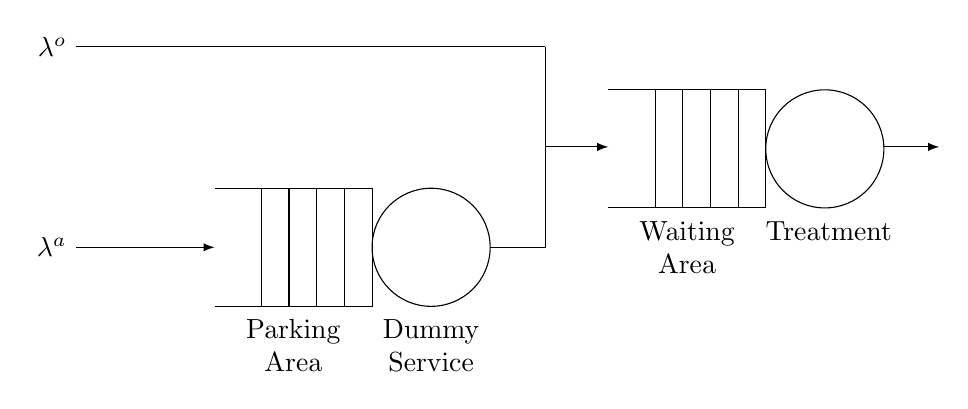
\begin{tikzpicture}[>=latex]
        % the rectangle with vertical rules (Queue 1)
        \draw (0,0) -- ++(2cm,0) -- ++(0,-1.5cm) -- ++(-2cm,0);
        \foreach \i in {1,...,4}
        \draw (2cm-\i*10pt,0) -- +(0,-1.5cm);
        
        % the circle (Queue 1)
        \draw (2.75,-0.75cm) circle [radius=0.75cm];

        % the rectangle with vertical rules (Queue 2)
        \draw (5,1.25) -- ++(2cm,0) -- ++(0,-1.5cm) -- ++(-2cm,0);
        \foreach \i in {1,...,4}
        \draw (7cm-\i*10pt,1.25) -- +(0,-1.5cm);

        % the circle (Queue 2)
        \draw (7.75,0.5) circle [radius=0.75cm];

        % the arrows and labels (Queue 1+2)
        \draw[-] (3.5,-0.75) -- +(20pt,0);
        \draw[<-] (0,-0.75) -- +(-50pt,0) node[left] {\( \lambda^a \)};
        \draw[->] (8.5,0.525) -- +(20pt,0);
        \node[align=center] at (1cm,-2cm) {Parking \\ Area};
        \node[align=center] at (2.75cm,-2cm) {Dummy \\ Service};
        \node[align=center] at (6cm,-0.75cm) {Waiting \\ Area};
        \node[align=center] at (7.8cm,-0.75cm) {Treatment \\ };
        
        \draw (4.2, 1.8) -- +(-169.5pt,0) node[left] {\( \lambda^o \)};
        \draw (4.2, 1.8) -- (4.2, -0.75);
        \draw[->] (4.2, 0.525) -- (5, 0.525);

    \end{tikzpicture}
\end{figure}


\begin{figure}
    \centering
    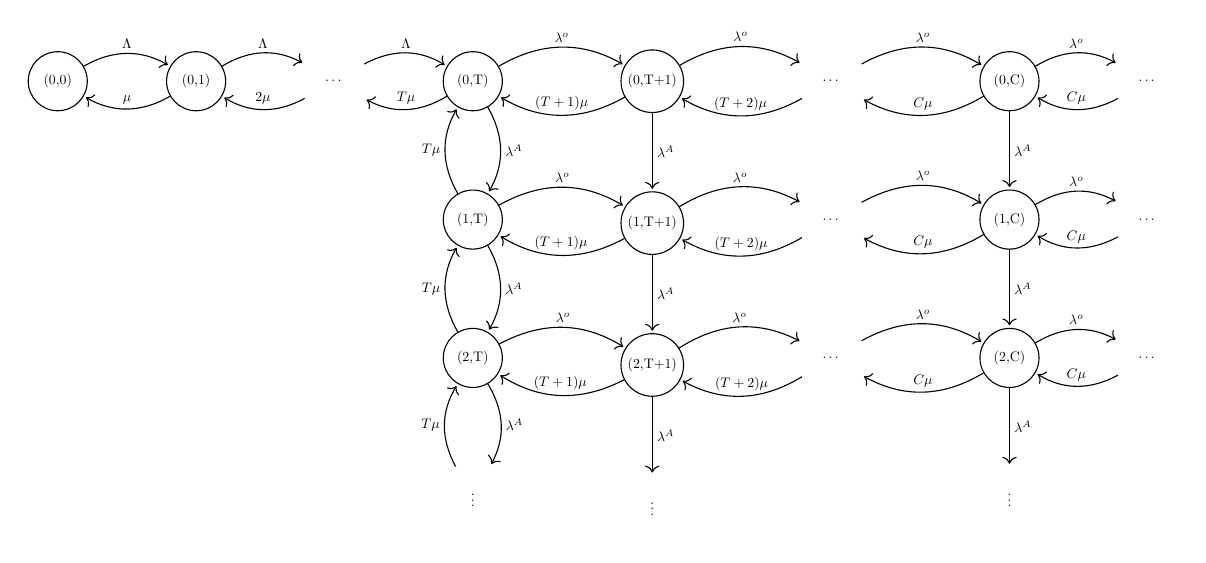
\begin{tikzpicture}[-, node distance = 1cm, auto, every node/.style={scale=0.5}]

        % Variables
        \tikzmath{
            let \altdist = 1.5cm;
            let \minsz = 1.5cm;
        }

        % First Line
        \node[state, minimum size=1.5cm] (zero) {(0,0)};
        \node[state, minimum size=1.5cm,  right=of zero] (one) {(0,1)};
        \node[draw=none, minimum size=1.5cm, right=of one] (two) {\dots};
        \node[state, minimum size=1.5cm, right=of two] (three) {(0,T)};
        \node[state, node distance = \altdist, minimum size=\minsz, right=of three] (four) {(0,T+1)};
        \node[draw=none, node distance = \altdist, minimum size=\minsz, right=of four] (five) {\dots};
        \node[state, node distance = \altdist, minimum size=\minsz, right=of five] (six) {(0,C)};
        \node[draw=none, minimum size=\minsz, right=of six] (seven) {\dots};

        % Second Line
        \node[state, minimum size=\minsz, below=of three] (three_one) {(1,T)};
        \node[state, minimum size=\minsz, below=of four] (four_one) {(1,T+1)};
        \node[draw=none, minimum size=\minsz, below=of five] (five_one) {\dots};
        \node[state, node distance = \altdist, minimum size=\minsz, right=of five_one] (six_one) {(1,C)};
        \node[draw=none, minimum size=\minsz, right=of six_one] (seven_one) {\dots};

        % Third Line
        \node[state, minimum size=\minsz, below=of three_one] (three_two) {(2,T)};
        \node[state, minimum size=\minsz, below=of four_one] (four_two) {(2,T+1)};
        \node[draw=none, minimum size=\minsz, below=of five_one] (five_two) {\dots};
        \node[state, node distance = \altdist, minimum size=\minsz, right=of five_two] (six_two) {(2,C)};
        \node[draw=none, minimum size=\minsz, right=of six_two] (seven_two) {\dots};

        % Fourth line
        \node[draw=none, minimum size=\minsz, below=of three_two] (three_three) {\vdots};
        \node[draw=none, minimum size=\minsz, below=of four_two] (four_three) {\vdots};
        \node[draw=none, minimum size=\minsz, below=of five_two] (five_three) {};
        \node[draw=none, node distance = \altdist, minimum size=\minsz, right=of five_three] (six_three) {\vdots};

        \draw[every loop]
            % First Horizontal Edges
            (zero) edge[bend left] node {\( \Lambda \)} (one)
            (one) edge[bend left] node [above] {\( \mu \)} (zero)
            (one) edge[bend left] node {\( \Lambda \)} (two)
            (two) edge[bend left] node [above] {\( 2 \mu \)} (one)
            (two) edge[bend left] node {\( \Lambda \)} (three)
            (three) edge[bend left] node [above] {\( T \mu \)} (two)
            (three) edge[bend left] node {\( \lambda^o \)} (four)
            (four) edge[bend left] node [above] {\( (T+1) \mu \)} (three)
            (four) edge[bend left] node {\( \lambda^o \)} (five)
            (five) edge[bend left] node [above] {\( (T+2) \mu \)} (four)
            (five) edge[bend left] node {\( \lambda^o \)} (six)
            (six) edge[bend left] node [above] {\( C\mu \)} (five)
            (six) edge[bend left] node {\( \lambda^o \)} (seven)
            (seven) edge[bend left] node [above] {\( C\mu \)} (six)

            % Second Horizontal Edges
            (three_one) edge[bend left] node {\( \lambda^o \)} (four_one)
            (four_one) edge[bend left] node [above] {\( (T+1) \mu \)} (three_one)
            (four_one) edge[bend left] node {\( \lambda^o \)} (five_one)
            (five_one) edge[bend left] node [above] {\( (T+2) \mu \)} (four_one)
            (five_one) edge[bend left] node {\( \lambda^o \)} (six_one)
            (six_one) edge[bend left] node [above] {\( C\mu \)} (five_one)
            (six_one) edge[bend left] node {\( \lambda^o \)} (seven_one)
            (seven_one) edge[bend left] node [above] {\( C\mu \)} (six_one)

            % Third Horizontal Edges
            (three_two) edge[bend left] node {\( \lambda^o \)} (four_two)
            (four_two) edge[bend left] node [above] {\( (T+1) \mu \)} (three_two)
            (four_two) edge[bend left] node {\( \lambda^o \)} (five_two)
            (five_two) edge[bend left] node [above] {\( (T+2) \mu \)} (four_two)
            (five_two) edge[bend left] node {\( \lambda^o \)} (six_two)
            (six_two) edge[bend left] node [above] {\( C\mu \)} (five_two)
            (six_two) edge[bend left] node {\( \lambda^o \)} (seven_two)
            (seven_two) edge[bend left] node [above] {\( C\mu \)} (six_two)

            % First Vertical Edges
            (three) edge[bend left] node {\( \lambda^A \)} (three_one)
            (three_one) edge[bend left] node {\( T \mu \)} (three)
            (three_one) edge[bend left] node {\( \lambda^A \)} (three_two)
            (three_two) edge[bend left] node {\( T\mu \)} (three_one)
            (three_two) edge[bend left] node {\( \lambda^A \)} (three_three)
            (three_three) edge[bend left] node {\( T\mu \)} (three_two)

            % Second Vertical Edges
            (four) edge node {\( \lambda^A \)} (four_one)
            (four_one) edge node {\( \lambda^A \)} (four_two)
            (four_two) edge node {\( \lambda^A \)} (four_three)

            %Third Vertical Edges
            (six) edge node {\( \lambda^A \)} (six_one)
            (six_one) edge node {\( \lambda^A \)} (six_two)
            (six_two) edge node {\( \lambda^A \)} (six_three)
            ;       
    \end{tikzpicture}
    \caption{Markov chains} 
    \label{Markov_2}
\end{figure}



\begin{figure}
    \centering
    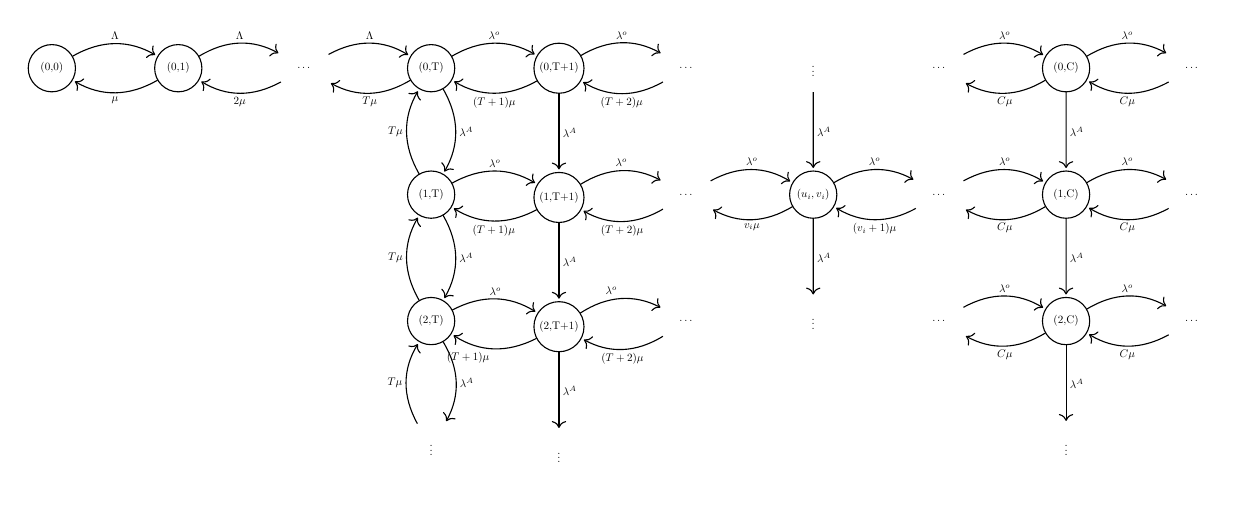
\begin{tikzpicture}[-, node distance = 1cm, auto, every node/.style={scale=0.4}]

        % Variables
        \tikzmath{
            let \altdist = 1cm;
            let \minsz = 1.5cm;
        }

        % First Line
        \node[state, minimum size=1.5cm] (zero) {(0,0)};
        \node[state, minimum size=1.5cm,  right=of zero] (one) {(0,1)};
        \node[draw=none, minimum size=1.5cm, right=of one] (two) {\dots};
        \node[state, minimum size=1.5cm, right=of two] (three) {(0,T)};
        \node[state, node distance = \altdist, minimum size=\minsz, right=of three] (four) {(0,T+1)};
        \node[draw=none, minimum size=\minsz, right=of four] (five) {\dots};
        \node[draw=none, minimum size=\minsz, right=of five] (six) {\vdots};
        \node[draw=none, minimum size=\minsz, right=of six] (seven) {\dots};
        \node[state, minimum size=\minsz, right=of seven] (eight) {(0,C)};
        \node[draw=none, minimum size=\minsz, right=of eight] (nine) {\dots};


        % Second Line
        \node[state, minimum size=\minsz, below=of three] (three_one) {(1,T)};
        \node[state, minimum size=\minsz, below=of four] (four_one) {(1,T+1)};
        \node[draw=none, minimum size=\minsz, below=of five] (five_one) {\dots};
        \node[state, node distance = \altdist, minimum size=\minsz, right=of five_one] (six_one) {\( (u_i, v_i) \)};
        \node[draw=none, minimum size=\minsz, right=of six_one] (seven_one) {\dots};
        \node[state, node distance = \altdist, minimum size=\minsz, right=of seven_one] (eight_one) {(1,C)};
        \node[draw=none, minimum size=\minsz, right=of eight_one] (nine_one) {\dots};
        

        % Third Line
        \node[state, minimum size=\minsz, below=of three_one] (three_two) {(2,T)};
        \node[state, minimum size=\minsz, below=of four_one] (four_two) {(2,T+1)};
        \node[draw=none, minimum size=\minsz, below=of five_one] (five_two) {\dots};
        \node[draw=none, node distance = \altdist, minimum size=\minsz, right=of five_two] (six_two) {\vdots};
        \node[draw=none, minimum size=\minsz, right=of six_two] (seven_two) {\dots};
        \node[state, node distance = \altdist, minimum size=\minsz, right=of seven_two] (eight_two) {(2,C)};
        \node[draw=none, minimum size=\minsz, right=of eight_two] (nine_two) {\dots};

        % Fourth line
        \node[draw=none, minimum size=\minsz, below=of three_two] (three_three) {\vdots};
        \node[draw=none, minimum size=\minsz, below=of four_two] (four_three) {\vdots};
        \node[draw=none, minimum size=\minsz, below=of five_two] (five_three) {};
        \node[draw=none, node distance = \altdist, minimum size=\minsz, right=of five_three] (six_three) {};
        \node[draw=none, node distance = \altdist, minimum size=\minsz, below=of eight_two] (eight_three) {\vdots};


        \draw[every loop]
            % First Horizontal Edges
            (zero) edge[bend left] node {\( \Lambda \)} (one)
            (one) edge[bend left] node {\( \mu \)} (zero)
            (one) edge[bend left] node {\( \Lambda \)} (two)
            (two) edge[bend left] node {\( 2 \mu \)} (one)
            (two) edge[bend left] node {\( \Lambda \)} (three)
            (three) edge[bend left] node {\( T \mu \)} (two)
            (three) edge[bend left] node {\( \lambda^o \)} (four)
            (four) edge[bend left] node {\( (T+1) \mu \)} (three)
            (four) edge[bend left] node {\( \lambda^o \)} (five)
            (five) edge[bend left] node {\( (T+2) \mu \)} (four)
            % (five) edge[bend left] node {\( \lambda^o \)} (six)
            % (six) edge[bend left] node [above] {\( C\mu \)} (five)
            % (six) edge[bend left] node {\( \lambda^o \)} (seven)
            % (seven) edge[bend left] node [above] {\( C\mu \)} (six)
            (seven) edge[bend left] node {\( \lambda^o \)} (eight)
            (eight) edge[bend left] node {\( C\mu \)} (seven)
            (eight) edge[bend left] node {\( \lambda^o \)} (nine)
            (nine) edge[bend left] node {\( C\mu \)} (eight)

            % Second Horizontal Edges
            (three_one) edge[bend left] node {\(\lambda^o\)} (four_one)
            (four_one) edge[bend left] node {\( (T+1) \mu \)} (three_one)
            (four_one) edge[bend left] node {\( \lambda^o \)} (five_one)
            (five_one) edge[bend left] node {\( (T+2) \mu \)} (four_one)
            (five_one) edge[bend left] node {\( \lambda^o \)} (six_one)
            (six_one) edge[bend left] node {\( v_i\mu \)} (five_one)
            (six_one) edge[bend left] node {\( \lambda^o \)} (seven_one)
            (seven_one) edge[bend left] node {\( (v_i+1)\mu \)} (six_one)
            (seven_one) edge[bend left] node {\( \lambda^o \)} (eight_one)
            (eight_one) edge[bend left] node {\( C\mu \)} (seven_one)
            (eight_one) edge[bend left] node {\( \lambda^o \)} (nine_one)
            (nine_one) edge[bend left] node {\( C\mu \)} (eight_one)

            % Third Horizontal Edges
            (three_two) edge[bend left] node {\( \lambda^o \)} (four_two)
            (four_two) edge[bend left] node {\( (T+1) \mu \)} (three_two)
            (four_two) edge[bend left] node {\( \lambda^o \)} (five_two)
            (five_two) edge[bend left] node {\( (T+2) \mu \)} (four_two)
            % (five_two) edge[bend left] node {\( \lambda^o \)} (six_two)
            % (six_two) edge[bend left] node [above] {\( C\mu \)} (five_two)
            % (six_two) edge[bend left] node {\( \lambda^o \)} (seven_two)
            % (seven_two) edge[bend left] node [above] {\( C\mu \)} (six_two)
            (seven_two) edge[bend left] node {\( \lambda^o \)} (eight_two)
            (eight_two) edge[bend left] node {\( C\mu \)} (seven_two)
            (eight_two) edge[bend left] node {\( \lambda^o \)} (nine_two)
            (nine_two) edge[bend left] node {\( C\mu \)} (eight_two)

            % First Vertical Edges
            (three) edge[bend left] node {\( \lambda^A \)} (three_one)
            (three_one) edge[bend left] node {\( T \mu \)} (three)
            (three_one) edge[bend left] node {\( \lambda^A \)} (three_two)
            (three_two) edge[bend left] node {\( T\mu \)} (three_one)
            (three_two) edge[bend left] node {\( \lambda^A \)} (three_three)
            (three_three) edge[bend left] node {\( T\mu \)} (three_two)

            % Second Vertical Edges
            (four) edge node {\( \lambda^A \)} (four_one)
            (four_one) edge node {\( \lambda^A \)} (four_two)
            (four_two) edge node {\( \lambda^A \)} (four_three)

            % Third Vertical Edges
            (six) edge node {\( \lambda^A \)} (six_one)
            (six_one) edge node {\( \lambda^A \)} (six_two)
            % (six_two) edge node {\( \lambda^A \)} (six_three)

            % Fourth Vertical Edges
            (eight) edge node {\( \lambda^A \)} (eight_one)
            (eight_one) edge node {\( \lambda^A \)} (eight_two)
            (eight_two) edge node {\( \lambda^A \)} (eight_three)
            ;       
    \end{tikzpicture}
    \caption{Markov chains} 
    \label{Markov_3}
\end{figure}


\begin{figure}
    \centering
    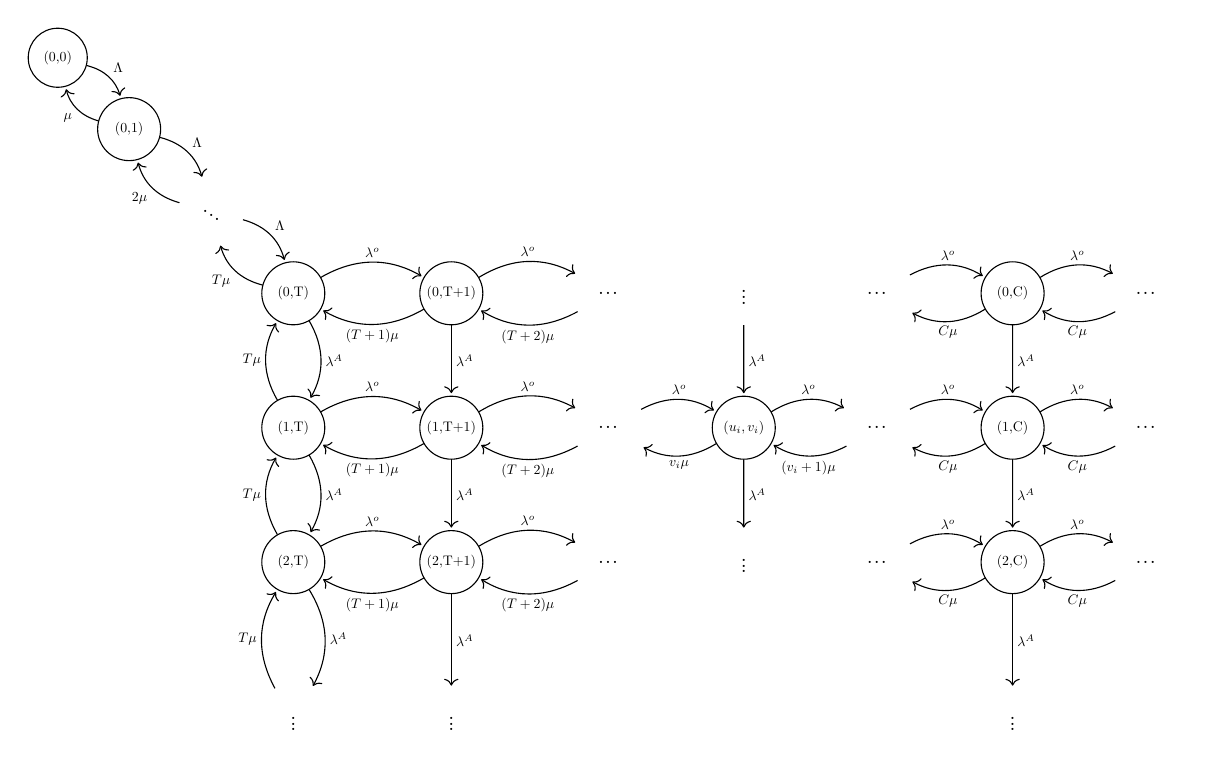
\begin{tikzpicture}[-, node distance = 0.9cm, auto, every node/.style={scale=0.5}]

        % Variables
        \tikzmath{
            let \initdist = 0.5cm;
            let \altdist = 1.2cm;
            let \minsz = 1.6cm;
            let \leftOne = -0.8;
            let \rightOne = 2.2;
            let \upOne = 0.8;
            let \downOne = -2.2;
            let \leftTwo = 2.25;
            let \rightTwo = 14.2;
            let \upTwo = -2.35;
            let \downTwo = -8.8;
        }

        % % Rectangle for S1
        % \draw[ultra thin, dashed] (\leftOne, \downOne) -- (\leftOne, \upOne);
        % \draw[ultra thin, dashed] (\leftOne, \upOne) -- (\rightOne, \upOne);
        % \draw[ultra thin, dashed] (\rightOne, \upOne) -- node {\Huge{\( \quad S_1 \)}}(\rightOne, \downOne);
        % \draw[ultra thin, dashed] (\rightOne, \downOne) -- (\leftOne, \downOne);

        % % Rectangle for S2
        % \draw[ultra thin, dashed] (\leftTwo, \downTwo) -- node {\Huge{\( S_2 \quad \)}}(\leftTwo, \upTwo);
        % \draw[ultra thin, dashed] (\leftTwo, \upTwo) -- (\rightTwo, \upTwo);
        % \draw[ultra thin, dashed] (\rightTwo, \upTwo) -- (\rightTwo, \downTwo);
        % \draw[ultra thin, dashed] (\rightTwo, \downTwo) -- (\leftTwo, \downTwo);

        % First Line
        \node[state, minimum size=1.5cm] (zero) {(0,0)};
        \node[state, node distance = \initdist, minimum size=\minsz, below right=of zero] (one) {(0,1)};
        \node[draw=none, node distance = \initdist, minimum size=\minsz, below right=of one] (two) {\textbf{\( \ddots \)}};
        \node[state, node distance = \initdist, minimum size=\minsz, below right=of two] (three) {(0,T)};
        \node[state, node distance = \altdist, minimum size=\minsz, right=of three] (four) {(0,T+1)};
        \node[draw=none, node distance = \altdist, minimum size=\minsz, right=of four] (five) {\textbf{\dots}};
        \node[draw=none, minimum size=\minsz, right=of five] (six) {\textbf{\vdots}};
        \node[draw=none, minimum size=\minsz, right=of six] (seven) {\textbf{\dots}};
        \node[state, minimum size=\minsz, right=of seven] (eight) {(0,C)};
        \node[draw=none, minimum size=\minsz, right=of eight] (nine) {\textbf{\dots}};


        % Second Line
        \node[state, minimum size=\minsz, below=of three] (three_one) {(1,T)};
        \node[state, minimum size=\minsz, below=of four] (four_one) {(1,T+1)};
        \node[draw=none, minimum size=\minsz, below=of five] (five_one) {\textbf{\dots}};
        \node[state, minimum size=\minsz, right=of five_one] (six_one) {\( (u_i, v_i) \)};
        \node[draw=none, minimum size=\minsz, right=of six_one] (seven_one) {\textbf{\dots}};
        \node[state, minimum size=\minsz, right=of seven_one] (eight_one) {(1,C)};
        \node[draw=none, minimum size=\minsz, right=of eight_one] (nine_one) {\textbf{\dots}};
        

        % Third Line
        \node[state, minimum size=\minsz, below=of three_one] (three_two) {(2,T)};
        \node[state, minimum size=\minsz, below=of four_one] (four_two) {(2,T+1)};
        \node[draw=none, minimum size=\minsz, below=of five_one] (five_two) {\textbf{\dots}};
        \node[draw=none, minimum size=\minsz, right=of five_two] (six_two) {\textbf{\vdots}};
        \node[draw=none, minimum size=\minsz, right=of six_two] (seven_two) {\textbf{\dots}};
        \node[state, minimum size=\minsz, right=of seven_two] (eight_two) {(2,C)};
        \node[draw=none, minimum size=\minsz, right=of eight_two] (nine_two) {\textbf{\dots}};

        % Fourth line
        \node[draw=none, node distance = \altdist, minimum size=\minsz, below=of three_two] (three_three) {\textbf{\vdots}};
        \node[draw=none, node distance = \altdist, minimum size=\minsz, below=of four_two] (four_three) {\textbf{\vdots}};
        \node[draw=none, node distance = \altdist, minimum size=\minsz, below=of five_two] (five_three) {};
        \node[draw=none, node distance = \altdist, minimum size=\minsz, below=of six_two] (six_three) {};
        \node[draw=none, node distance = \altdist, minimum size=\minsz, below=of eight_two] (eight_three) {\textbf{\vdots}};


        \draw[every loop]
            % First Horizontal Edges
            (zero) edge[bend left] node {\( \Lambda \)} (one)
            (one) edge[bend left] node {\( \mu \)} (zero)
            (one) edge[bend left] node {\( \Lambda \)} (two)
            (two) edge[bend left] node {\( 2 \mu \)} (one)
            (two) edge[bend left] node {\( \Lambda \)} (three)
            (three) edge[bend left] node {\( T \mu \)} (two)
            (three) edge[bend left] node {\( \lambda^o \)} (four)
            (four) edge[bend left] node {\( (T+1) \mu \)} (three)
            (four) edge[bend left] node {\( \lambda^o \)} (five)
            (five) edge[bend left] node {\( (T+2) \mu \)} (four)
            % (five) edge[bend left] node {\( \lambda^o \)} (six)
            % (six) edge[bend left] node [above] {\( C\mu \)} (five)
            % (six) edge[bend left] node {\( \lambda^o \)} (seven)
            % (seven) edge[bend left] node [above] {\( C\mu \)} (six)
            (seven) edge[bend left] node {\( \lambda^o \)} (eight)
            (eight) edge[bend left] node {\( C\mu \)} (seven)
            (eight) edge[bend left] node {\( \lambda^o \)} (nine)
            (nine) edge[bend left] node {\( C\mu \)} (eight)

            % Second Horizontal Edges
            (three_one) edge[bend left] node {\( \lambda^o \)} (four_one)
            (four_one) edge[bend left] node {\( (T+1) \mu \)} (three_one)
            (four_one) edge[bend left] node {\( \lambda^o \)} (five_one)
            (five_one) edge[bend left] node {\( (T+2) \mu \)} (four_one)
            (five_one) edge[bend left] node {\( \lambda^o \)} (six_one)
            (six_one) edge[bend left] node {\( v_i\mu \)} (five_one)
            (six_one) edge[bend left] node {\( \lambda^o \)} (seven_one)
            (seven_one) edge[bend left] node {\( (v_i+1)\mu \)} (six_one)
            (seven_one) edge[bend left] node {\( \lambda^o \)} (eight_one)
            (eight_one) edge[bend left] node {\( C\mu \)} (seven_one)
            (eight_one) edge[bend left] node {\( \lambda^o \)} (nine_one)
            (nine_one) edge[bend left] node {\( C\mu \)} (eight_one)

            % Third Horizontal Edges
            (three_two) edge[bend left] node {\( \lambda^o \)} (four_two)
            (four_two) edge[bend left] node [below] {\( (T+1) \mu \)} (three_two)
            (four_two) edge[bend left] node {\( \lambda^o \)} (five_two)
            (five_two) edge[bend left] node {\( (T+2) \mu \)} (four_two)
            % (five_two) edge[bend left] node {\( \lambda^o \)} (six_two)
            % (six_two) edge[bend left] node [above] {\( C\mu \)} (five_two)
            % (six_two) edge[bend left] node {\( \lambda^o \)} (seven_two)
            % (seven_two) edge[bend left] node [above] {\( C\mu \)} (six_two)
            (seven_two) edge[bend left] node {\( \lambda^o \)} (eight_two)
            (eight_two) edge[bend left] node {\( C\mu \)} (seven_two)
            (eight_two) edge[bend left] node {\( \lambda^o \)} (nine_two)
            (nine_two) edge[bend left] node {\( C\mu \)} (eight_two)

            % First Vertical Edges
            (three) edge[bend left] node {\( \lambda^A \)} (three_one)
            (three_one) edge[bend left] node {\( T \mu \)} (three)
            (three_one) edge[bend left] node {\( \lambda^A \)} (three_two)
            (three_two) edge[bend left] node {\( T\mu \)} (three_one)
            (three_two) edge[bend left] node {\( \lambda^A \)} (three_three)
            (three_three) edge[bend left] node {\( T\mu \)} (three_two)

            % Second Vertical Edges
            (four) edge node {\( \lambda^A \)} (four_one)
            (four_one) edge node {\( \lambda^A \)} (four_two)
            (four_two) edge node {\( \lambda^A \)} (four_three)

            % Third Vertical Edges
            (six) edge node {\( \lambda^A \)} (six_one)
            (six_one) edge node {\( \lambda^A \)} (six_two)
            % (six_two) edge node {\( \lambda^A \)} (six_three)

            % Fourth Vertical Edges
            (eight) edge node {\( \lambda^A \)} (eight_one)
            (eight_one) edge node {\( \lambda^A \)} (eight_two)
            (eight_two) edge node {\( \lambda^A \)} (eight_three)
            ;       
    \end{tikzpicture}
    \caption{Markov chains} 
    \label{Markov_4}
\end{figure}




\begin{figure}
    \centering
    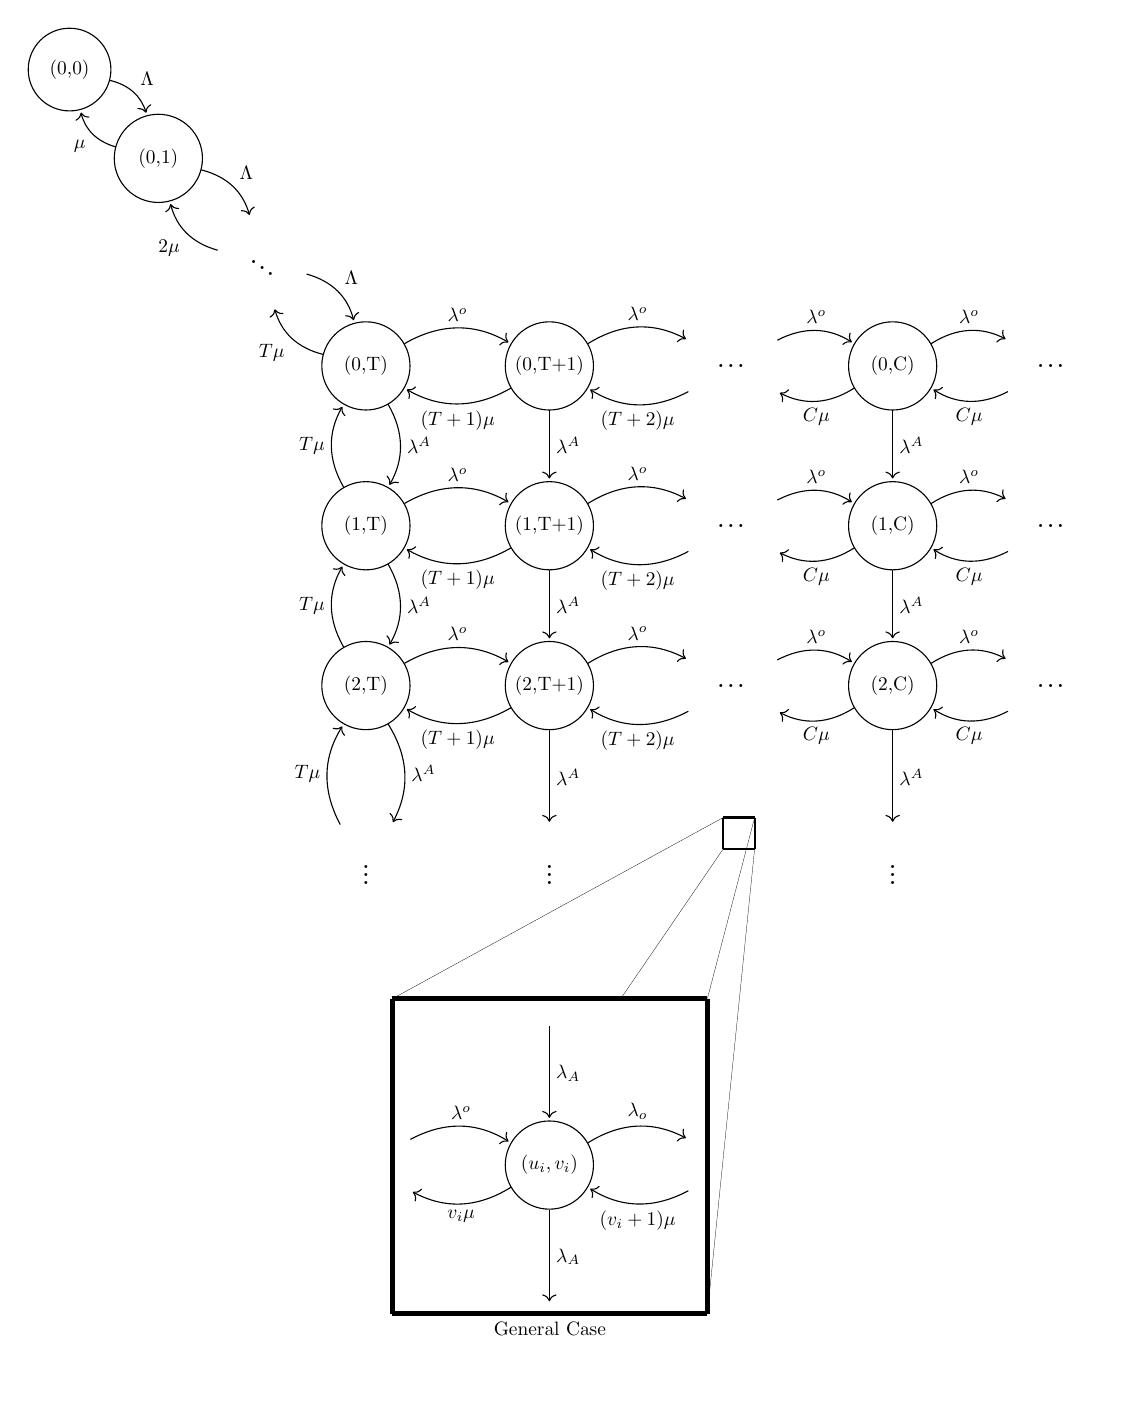
\begin{tikzpicture}[-, node distance = 0.9cm, auto, every node/.style={scale=0.7}]

        % Markov chain variables
        \tikzmath{
            let \initdist = 0.5cm;
            let \altdist = 1.2cm;
            let \minsz = 1.6cm;
        }

        % S_1 and S_2 rectangles
        \tikzmath{
            let \leftOne = -0.8;
            let \rightOne = 2.7;
            let \upOne = 0.8;
            let \downOne = -2.7;
            let \leftTwo = 2.8;
            let \rightTwo = 13;
            let \upTwo = -2.95;
            let \downTwo = -16.4;
        }

        % General case variables
        \tikzmath{
            let \GCsmallx = 8.3;
            let \GCsmally = -9.5;
            let \GCbigx = 4.1;
            let \GCbigy = -11.8;
        }

        % % Rectangle for S1
        % \draw[ultra thin, dashed] (\leftOne, \downOne) -- (\leftOne, \upOne);
        % \draw[ultra thin, dashed] (\leftOne, \upOne) -- (\rightOne, \upOne);
        % \draw[ultra thin, dashed] (\rightOne, \upOne) -- node {\Huge{\( \quad S_1 \)}}(\rightOne, \downOne);
        % \draw[ultra thin, dashed] (\rightOne, \downOne) -- (\leftOne, \downOne);

        % % Rectangle for S2
        % \draw[ultra thin, dashed] (\leftTwo, \downTwo) -- node {\Huge{\( S_2 \quad \)}}(\leftTwo, \upTwo);
        % \draw[ultra thin, dashed] (\leftTwo, \upTwo) -- (\rightTwo, \upTwo);
        % \draw[ultra thin, dashed] (\rightTwo, \upTwo) -- (\rightTwo, \downTwo);
        % \draw[ultra thin, dashed] (\rightTwo, \downTwo) -- (\leftTwo, \downTwo);

        % Small square of general case
        \draw [thick] (\GCsmallx, \GCsmally) -- node {} (\GCsmallx + 0.4, \GCsmally);
        \draw [thick] (\GCsmallx + 0.4, \GCsmally) -- node {} (\GCsmallx + 0.4, \GCsmally - 0.4);
        \draw [thick] (\GCsmallx + 0.4, \GCsmally - 0.4) -- node {} (\GCsmallx, \GCsmally - 0.4);
        \draw [thick] (\GCsmallx, \GCsmally - 0.4) -- node {} (\GCsmallx, \GCsmally);


        % Dashed lines to from small square to big one 
        \draw [ultra thin] (\GCsmallx, \GCsmally) -- node {} (\GCbigx, \GCbigy);
        \draw [ultra thin] (\GCsmallx + 0.4, \GCsmally) -- node {} (\GCbigx + 4, \GCbigy);
        \draw [ultra thin] (\GCsmallx, \GCsmally - 0.4) -- node {} (7, \GCbigy);
        \draw [ultra thin] (\GCsmallx + 0.4, \GCsmally - 0.4) -- node {} (\GCbigx + 4, \GCbigy - 4);
        
        % Big Square of general case
        \draw [ultra thick] (\GCbigx, \GCbigy) -- node {} (\GCbigx + 4, \GCbigy);
        \draw [ultra thick] (\GCbigx + 4, \GCbigy) -- node {} (\GCbigx + 4, \GCbigy - 4);
        \draw [ultra thick] (\GCbigx + 4, \GCbigy - 4) -- node {General Case} (\GCbigx, \GCbigy - 4);
        \draw [ultra thick] (\GCbigx, \GCbigy - 4) -- node {} (\GCbigx, \GCbigy);

        % First Line
        \node[state, minimum size=1.5cm] (zero) {(0,0)};
        \node[state, node distance = \initdist, minimum size=\minsz, below right=of zero] (one) {(0,1)};
        \node[draw=none, node distance = \initdist, minimum size=\minsz, below right=of one] (two) {\textbf{\( \ddots \)}};
        \node[state, node distance = \initdist, minimum size=\minsz, below right=of two] (three) {(0,T)};
        \node[state, node distance = \altdist, minimum size=\minsz, right=of three] (four) {(0,T+1)};
        \node[draw=none, node distance = \altdist, minimum size=\minsz, right=of four] (five) {\textbf{\dots}};
        \node[state, minimum size=\minsz, right=of five] (six) {(0,C)};
        \node[draw=none, minimum size=\minsz, right=of six] (seven) {\textbf{\dots}};

        % Second Line
        \node[state, minimum size=\minsz, below=of three] (three_one) {(1,T)};
        \node[state, minimum size=\minsz, below=of four] (four_one) {(1,T+1)};
        \node[draw=none, minimum size=\minsz, below=of five] (five_one) {\textbf{\dots}};
        \node[state, minimum size=\minsz, right=of five_one] (six_one) {(1,C)};
        \node[draw=none, minimum size=\minsz, right=of six_one] (seven_one) {\textbf{\dots}};
        
        % Third Line
        \node[state, minimum size=\minsz, below=of three_one] (three_two) {(2,T)};
        \node[state, minimum size=\minsz, below=of four_one] (four_two) {(2,T+1)};
        \node[draw=none, minimum size=\minsz, below=of five_one] (five_two) {\textbf{\dots}};
        \node[state, minimum size=\minsz, right=of five_two] (six_two) {(2,C)};
        \node[draw=none, minimum size=\minsz, right=of six_two] (seven_two) {\textbf{\dots}};

        % Fourth line
        \node[draw=none, node distance = \altdist, minimum size=\minsz, below=of three_two] (three_three) {\textbf{\vdots}};
        \node[draw=none, node distance = \altdist, minimum size=\minsz, below=of four_two] (four_three) {\textbf{\vdots}};
        \node[draw=none, node distance = 2cm, minimum size=\minsz, below=of five_two] (five_three) {};
        \node[draw=none, node distance = \altdist, minimum size=\minsz, below=of six_two] (six_three) {\textbf{\vdots}};

        % Fifth line
        % \node[state, node distance = \altdist, minimum size=\minsz, below=of five_three] (general_case_mid) {\( (u_i, v_i) \)};
        \node[draw=none, node distance = 0.3cm, minimum size=\minsz, below=of four_three] (general_case_up) {};
        \node[state, node distance = \altdist, minimum size=\minsz, below=of general_case_up] (general_case_mid) {\( (u_i, v_i) \)};

        \node[draw=none, node distance = \altdist, minimum size=\minsz, below=of general_case_mid] (general_case_down) {};
        \node[draw=none, node distance = \altdist, minimum size=\minsz, left=of general_case_mid] (general_case_left) {};
        \node[draw=none, node distance = \altdist, minimum size=\minsz, right=of general_case_mid] (general_case_right) {};

        \draw[every loop]
            % First Horizontal Edges
            (zero) edge[bend left] node {\( \Lambda \)} (one)
            (one) edge[bend left] node {\( \mu \)} (zero)
            (one) edge[bend left] node {\( \Lambda \)} (two)
            (two) edge[bend left] node {\( 2 \mu \)} (one)
            (two) edge[bend left] node {\( \Lambda \)} (three)
            (three) edge[bend left] node {\( T \mu \)} (two)
            (three) edge[bend left] node {\( \lambda^o \)} (four)
            (four) edge[bend left] node {\( (T+1) \mu \)} (three)
            (four) edge[bend left] node {\( \lambda^o \)} (five)
            (five) edge[bend left] node {\( (T+2) \mu \)} (four)
            (five) edge[bend left] node {\( \lambda^o \)} (six)
            (six) edge[bend left] node {\( C\mu \)} (five)
            (six) edge[bend left] node {\( \lambda^o \)} (seven)
            (seven) edge[bend left] node {\( C\mu \)} (six)

            % Second Horizontal Edges
            (three_one) edge[bend left] node {\( \lambda^o \)} (four_one)
            (four_one) edge[bend left] node {\( (T+1) \mu \)} (three_one)
            (four_one) edge[bend left] node {\( \lambda^o \)} (five_one)
            (five_one) edge[bend left] node {\( (T+2) \mu \)} (four_one)
            (five_one) edge[bend left] node {\( \lambda^o \)} (six_one)
            (six_one) edge[bend left] node {\( C\mu \)} (five_one)
            (six_one) edge[bend left] node {\( \lambda^o \)} (seven_one)
            (seven_one) edge[bend left] node {\( C\mu \)} (six_one)

            % Third Horizontal Edges
            (three_two) edge[bend left] node {\( \lambda^o \)} (four_two)
            (four_two) edge[bend left] node [below] {\( (T+1) \mu \)} (three_two)
            (four_two) edge[bend left] node {\( \lambda^o \)} (five_two)
            (five_two) edge[bend left] node {\( (T+2) \mu \)} (four_two)
            (five_two) edge[bend left] node {\( \lambda^o \)} (six_two)
            (six_two) edge[bend left] node {\( C\mu \)} (five_two)
            (six_two) edge[bend left] node {\( \lambda^o \)} (seven_two)
            (seven_two) edge[bend left] node {\( C\mu \)} (six_two)

            % First Vertical Edges
            (three) edge[bend left] node {\( \lambda^A \)} (three_one)
            (three_one) edge[bend left] node {\( T \mu \)} (three)
            (three_one) edge[bend left] node {\( \lambda^A \)} (three_two)
            (three_two) edge[bend left] node {\( T\mu \)} (three_one)
            (three_two) edge[bend left] node {\( \lambda^A \)} (three_three)
            (three_three) edge[bend left] node {\( T\mu \)} (three_two)

            % Second Vertical Edges
            (four) edge node {\( \lambda^A \)} (four_one)
            (four_one) edge node {\( \lambda^A \)} (four_two)
            (four_two) edge node {\( \lambda^A \)} (four_three)

            % Fourth Vertical Edges
            (six) edge node {\( \lambda^A \)} (six_one)
            (six_one) edge node {\( \lambda^A \)} (six_two)
            (six_two) edge node {\( \lambda^A \)} (six_three)

            % General Case
            (general_case_left) edge[bend left] node {\( \lambda^o \)} (general_case_mid)
            (general_case_mid) edge[bend left] node {\( v_i \mu \)} (general_case_left)
            (general_case_right) edge[bend left] node {\( (v_i +1) \mu \)} (general_case_mid)
            (general_case_mid) edge[bend left] node {\( \lambda_o \)} (general_case_right)
            % (five_three) edge node {\( \lambda_A \)} (general_case_mid)
            (general_case_up) edge node {\( \lambda_A \)} (general_case_mid)
            (general_case_mid) edge node {\( \lambda_A \)} (general_case_down)
            ;
    \end{tikzpicture}
    \caption{Markov chain} 
    \label{Markov_5}
\end{figure}



% Game Theoretic Component
\section{Figures that might be useful}
\begin{figure}[h]
    \centering
    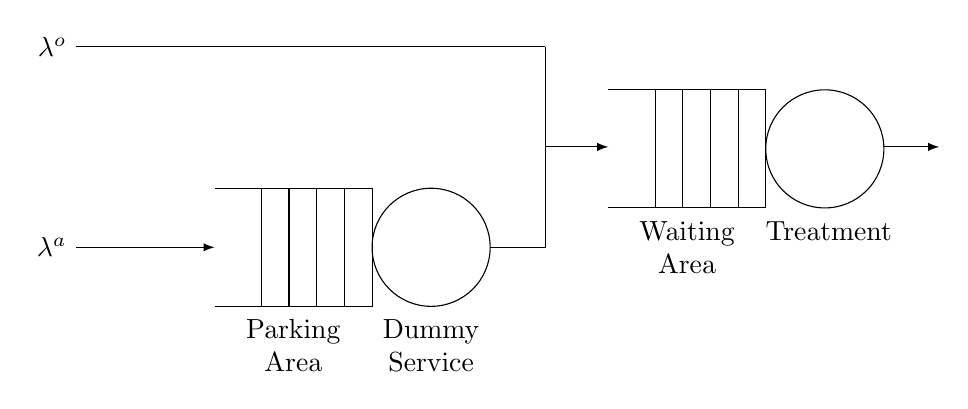
\begin{tikzpicture}[>=latex]
        % the rectangle with vertical rules (Queue 1)
        \draw (0,0) -- ++(2cm,0) -- ++(0,-1.5cm) -- ++(-2cm,0);
        \foreach \i in {1,...,4}
        \draw (2cm-\i*10pt,0) -- +(0,-1.5cm);
        
        % the circle (Queue 1)
        \draw (2.75,-0.75cm) circle [radius=0.75cm];

        % the rectangle with vertical rules (Queue 2)
        \draw (5,1.25) -- ++(2cm,0) -- ++(0,-1.5cm) -- ++(-2cm,0);
        \foreach \i in {1,...,4}
        \draw (7cm-\i*10pt,1.25) -- +(0,-1.5cm);

        % the circle (Queue 2)
        \draw (7.75,0.5) circle [radius=0.75cm];

        % the arrows and labels (Queue 1+2)
        \draw[-] (3.5,-0.75) -- +(20pt,0);
        \draw[<-] (0,-0.75) -- +(-50pt,0) node[left] {\( \lambda^a \)};
        \draw[->] (8.5,0.525) -- +(20pt,0);
        \node[align=center] at (1cm,-2cm) {Parking \\ Area};
        \node[align=center] at (2.75cm,-2cm) {Dummy \\ Service};
        \node[align=center] at (6cm,-0.75cm) {Waiting \\ Area};
        \node[align=center] at (7.8cm,-0.75cm) {Treatment \\ };
        
        \draw (4.2, 1.8) -- +(-169.5pt,0) node[left] {\( \lambda^o \)};
        \draw (4.2, 1.8) -- (4.2, -0.75);
        \draw[->] (4.2, 0.525) -- (5, 0.525);

    \end{tikzpicture}
\end{figure}


\begin{figure}
    \centering
    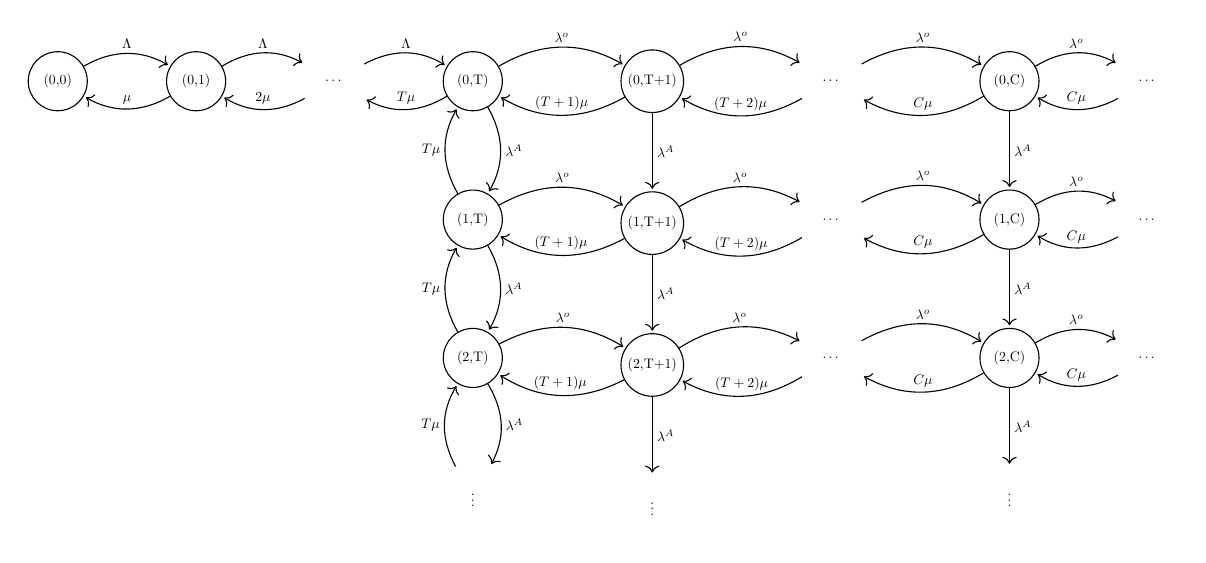
\begin{tikzpicture}[-, node distance = 1cm, auto, every node/.style={scale=0.5}]

        % Variables
        \tikzmath{
            let \altdist = 1.5cm;
            let \minsz = 1.5cm;
        }

        % First Line
        \node[state, minimum size=1.5cm] (zero) {(0,0)};
        \node[state, minimum size=1.5cm,  right=of zero] (one) {(0,1)};
        \node[draw=none, minimum size=1.5cm, right=of one] (two) {\dots};
        \node[state, minimum size=1.5cm, right=of two] (three) {(0,T)};
        \node[state, node distance = \altdist, minimum size=\minsz, right=of three] (four) {(0,T+1)};
        \node[draw=none, node distance = \altdist, minimum size=\minsz, right=of four] (five) {\dots};
        \node[state, node distance = \altdist, minimum size=\minsz, right=of five] (six) {(0,C)};
        \node[draw=none, minimum size=\minsz, right=of six] (seven) {\dots};

        % Second Line
        \node[state, minimum size=\minsz, below=of three] (three_one) {(1,T)};
        \node[state, minimum size=\minsz, below=of four] (four_one) {(1,T+1)};
        \node[draw=none, minimum size=\minsz, below=of five] (five_one) {\dots};
        \node[state, node distance = \altdist, minimum size=\minsz, right=of five_one] (six_one) {(1,C)};
        \node[draw=none, minimum size=\minsz, right=of six_one] (seven_one) {\dots};

        % Third Line
        \node[state, minimum size=\minsz, below=of three_one] (three_two) {(2,T)};
        \node[state, minimum size=\minsz, below=of four_one] (four_two) {(2,T+1)};
        \node[draw=none, minimum size=\minsz, below=of five_one] (five_two) {\dots};
        \node[state, node distance = \altdist, minimum size=\minsz, right=of five_two] (six_two) {(2,C)};
        \node[draw=none, minimum size=\minsz, right=of six_two] (seven_two) {\dots};

        % Fourth line
        \node[draw=none, minimum size=\minsz, below=of three_two] (three_three) {\vdots};
        \node[draw=none, minimum size=\minsz, below=of four_two] (four_three) {\vdots};
        \node[draw=none, minimum size=\minsz, below=of five_two] (five_three) {};
        \node[draw=none, node distance = \altdist, minimum size=\minsz, right=of five_three] (six_three) {\vdots};

        \draw[every loop]
            % First Horizontal Edges
            (zero) edge[bend left] node {\( \Lambda \)} (one)
            (one) edge[bend left] node [above] {\( \mu \)} (zero)
            (one) edge[bend left] node {\( \Lambda \)} (two)
            (two) edge[bend left] node [above] {\( 2 \mu \)} (one)
            (two) edge[bend left] node {\( \Lambda \)} (three)
            (three) edge[bend left] node [above] {\( T \mu \)} (two)
            (three) edge[bend left] node {\( \lambda^o \)} (four)
            (four) edge[bend left] node [above] {\( (T+1) \mu \)} (three)
            (four) edge[bend left] node {\( \lambda^o \)} (five)
            (five) edge[bend left] node [above] {\( (T+2) \mu \)} (four)
            (five) edge[bend left] node {\( \lambda^o \)} (six)
            (six) edge[bend left] node [above] {\( C\mu \)} (five)
            (six) edge[bend left] node {\( \lambda^o \)} (seven)
            (seven) edge[bend left] node [above] {\( C\mu \)} (six)

            % Second Horizontal Edges
            (three_one) edge[bend left] node {\( \lambda^o \)} (four_one)
            (four_one) edge[bend left] node [above] {\( (T+1) \mu \)} (three_one)
            (four_one) edge[bend left] node {\( \lambda^o \)} (five_one)
            (five_one) edge[bend left] node [above] {\( (T+2) \mu \)} (four_one)
            (five_one) edge[bend left] node {\( \lambda^o \)} (six_one)
            (six_one) edge[bend left] node [above] {\( C\mu \)} (five_one)
            (six_one) edge[bend left] node {\( \lambda^o \)} (seven_one)
            (seven_one) edge[bend left] node [above] {\( C\mu \)} (six_one)

            % Third Horizontal Edges
            (three_two) edge[bend left] node {\( \lambda^o \)} (four_two)
            (four_two) edge[bend left] node [above] {\( (T+1) \mu \)} (three_two)
            (four_two) edge[bend left] node {\( \lambda^o \)} (five_two)
            (five_two) edge[bend left] node [above] {\( (T+2) \mu \)} (four_two)
            (five_two) edge[bend left] node {\( \lambda^o \)} (six_two)
            (six_two) edge[bend left] node [above] {\( C\mu \)} (five_two)
            (six_two) edge[bend left] node {\( \lambda^o \)} (seven_two)
            (seven_two) edge[bend left] node [above] {\( C\mu \)} (six_two)

            % First Vertical Edges
            (three) edge[bend left] node {\( \lambda^A \)} (three_one)
            (three_one) edge[bend left] node {\( T \mu \)} (three)
            (three_one) edge[bend left] node {\( \lambda^A \)} (three_two)
            (three_two) edge[bend left] node {\( T\mu \)} (three_one)
            (three_two) edge[bend left] node {\( \lambda^A \)} (three_three)
            (three_three) edge[bend left] node {\( T\mu \)} (three_two)

            % Second Vertical Edges
            (four) edge node {\( \lambda^A \)} (four_one)
            (four_one) edge node {\( \lambda^A \)} (four_two)
            (four_two) edge node {\( \lambda^A \)} (four_three)

            %Third Vertical Edges
            (six) edge node {\( \lambda^A \)} (six_one)
            (six_one) edge node {\( \lambda^A \)} (six_two)
            (six_two) edge node {\( \lambda^A \)} (six_three)
            ;       
    \end{tikzpicture}
    \caption{Markov chains} 
    \label{Markov_2}
\end{figure}



\begin{figure}
    \centering
    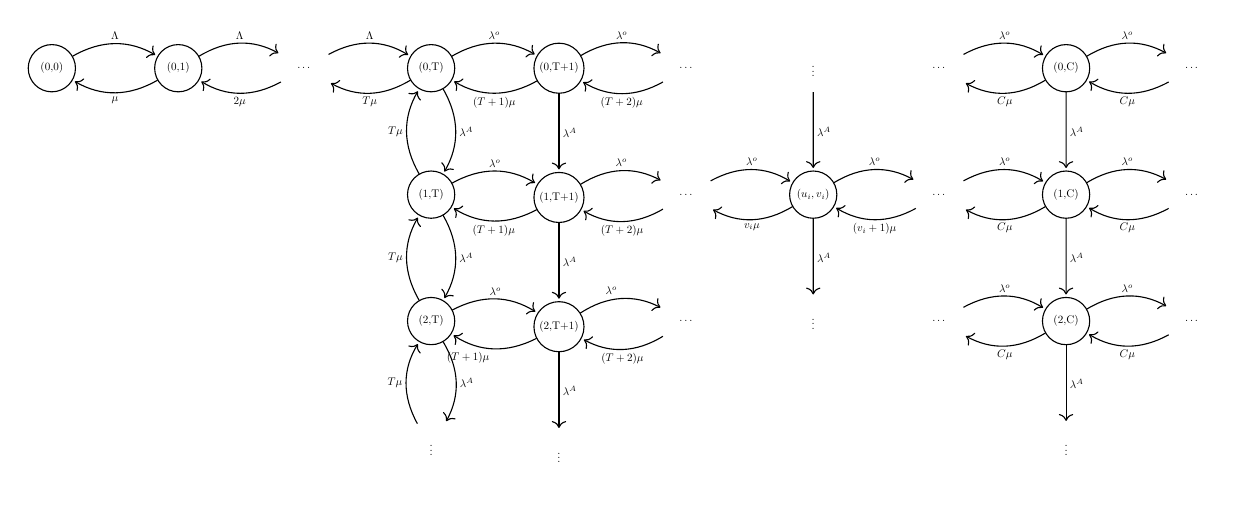
\begin{tikzpicture}[-, node distance = 1cm, auto, every node/.style={scale=0.4}]

        % Variables
        \tikzmath{
            let \altdist = 1cm;
            let \minsz = 1.5cm;
        }

        % First Line
        \node[state, minimum size=1.5cm] (zero) {(0,0)};
        \node[state, minimum size=1.5cm,  right=of zero] (one) {(0,1)};
        \node[draw=none, minimum size=1.5cm, right=of one] (two) {\dots};
        \node[state, minimum size=1.5cm, right=of two] (three) {(0,T)};
        \node[state, node distance = \altdist, minimum size=\minsz, right=of three] (four) {(0,T+1)};
        \node[draw=none, minimum size=\minsz, right=of four] (five) {\dots};
        \node[draw=none, minimum size=\minsz, right=of five] (six) {\vdots};
        \node[draw=none, minimum size=\minsz, right=of six] (seven) {\dots};
        \node[state, minimum size=\minsz, right=of seven] (eight) {(0,C)};
        \node[draw=none, minimum size=\minsz, right=of eight] (nine) {\dots};


        % Second Line
        \node[state, minimum size=\minsz, below=of three] (three_one) {(1,T)};
        \node[state, minimum size=\minsz, below=of four] (four_one) {(1,T+1)};
        \node[draw=none, minimum size=\minsz, below=of five] (five_one) {\dots};
        \node[state, node distance = \altdist, minimum size=\minsz, right=of five_one] (six_one) {\( (u_i, v_i) \)};
        \node[draw=none, minimum size=\minsz, right=of six_one] (seven_one) {\dots};
        \node[state, node distance = \altdist, minimum size=\minsz, right=of seven_one] (eight_one) {(1,C)};
        \node[draw=none, minimum size=\minsz, right=of eight_one] (nine_one) {\dots};
        

        % Third Line
        \node[state, minimum size=\minsz, below=of three_one] (three_two) {(2,T)};
        \node[state, minimum size=\minsz, below=of four_one] (four_two) {(2,T+1)};
        \node[draw=none, minimum size=\minsz, below=of five_one] (five_two) {\dots};
        \node[draw=none, node distance = \altdist, minimum size=\minsz, right=of five_two] (six_two) {\vdots};
        \node[draw=none, minimum size=\minsz, right=of six_two] (seven_two) {\dots};
        \node[state, node distance = \altdist, minimum size=\minsz, right=of seven_two] (eight_two) {(2,C)};
        \node[draw=none, minimum size=\minsz, right=of eight_two] (nine_two) {\dots};

        % Fourth line
        \node[draw=none, minimum size=\minsz, below=of three_two] (three_three) {\vdots};
        \node[draw=none, minimum size=\minsz, below=of four_two] (four_three) {\vdots};
        \node[draw=none, minimum size=\minsz, below=of five_two] (five_three) {};
        \node[draw=none, node distance = \altdist, minimum size=\minsz, right=of five_three] (six_three) {};
        \node[draw=none, node distance = \altdist, minimum size=\minsz, below=of eight_two] (eight_three) {\vdots};


        \draw[every loop]
            % First Horizontal Edges
            (zero) edge[bend left] node {\( \Lambda \)} (one)
            (one) edge[bend left] node {\( \mu \)} (zero)
            (one) edge[bend left] node {\( \Lambda \)} (two)
            (two) edge[bend left] node {\( 2 \mu \)} (one)
            (two) edge[bend left] node {\( \Lambda \)} (three)
            (three) edge[bend left] node {\( T \mu \)} (two)
            (three) edge[bend left] node {\( \lambda^o \)} (four)
            (four) edge[bend left] node {\( (T+1) \mu \)} (three)
            (four) edge[bend left] node {\( \lambda^o \)} (five)
            (five) edge[bend left] node {\( (T+2) \mu \)} (four)
            % (five) edge[bend left] node {\( \lambda^o \)} (six)
            % (six) edge[bend left] node [above] {\( C\mu \)} (five)
            % (six) edge[bend left] node {\( \lambda^o \)} (seven)
            % (seven) edge[bend left] node [above] {\( C\mu \)} (six)
            (seven) edge[bend left] node {\( \lambda^o \)} (eight)
            (eight) edge[bend left] node {\( C\mu \)} (seven)
            (eight) edge[bend left] node {\( \lambda^o \)} (nine)
            (nine) edge[bend left] node {\( C\mu \)} (eight)

            % Second Horizontal Edges
            (three_one) edge[bend left] node {\(\lambda^o\)} (four_one)
            (four_one) edge[bend left] node {\( (T+1) \mu \)} (three_one)
            (four_one) edge[bend left] node {\( \lambda^o \)} (five_one)
            (five_one) edge[bend left] node {\( (T+2) \mu \)} (four_one)
            (five_one) edge[bend left] node {\( \lambda^o \)} (six_one)
            (six_one) edge[bend left] node {\( v_i\mu \)} (five_one)
            (six_one) edge[bend left] node {\( \lambda^o \)} (seven_one)
            (seven_one) edge[bend left] node {\( (v_i+1)\mu \)} (six_one)
            (seven_one) edge[bend left] node {\( \lambda^o \)} (eight_one)
            (eight_one) edge[bend left] node {\( C\mu \)} (seven_one)
            (eight_one) edge[bend left] node {\( \lambda^o \)} (nine_one)
            (nine_one) edge[bend left] node {\( C\mu \)} (eight_one)

            % Third Horizontal Edges
            (three_two) edge[bend left] node {\( \lambda^o \)} (four_two)
            (four_two) edge[bend left] node {\( (T+1) \mu \)} (three_two)
            (four_two) edge[bend left] node {\( \lambda^o \)} (five_two)
            (five_two) edge[bend left] node {\( (T+2) \mu \)} (four_two)
            % (five_two) edge[bend left] node {\( \lambda^o \)} (six_two)
            % (six_two) edge[bend left] node [above] {\( C\mu \)} (five_two)
            % (six_two) edge[bend left] node {\( \lambda^o \)} (seven_two)
            % (seven_two) edge[bend left] node [above] {\( C\mu \)} (six_two)
            (seven_two) edge[bend left] node {\( \lambda^o \)} (eight_two)
            (eight_two) edge[bend left] node {\( C\mu \)} (seven_two)
            (eight_two) edge[bend left] node {\( \lambda^o \)} (nine_two)
            (nine_two) edge[bend left] node {\( C\mu \)} (eight_two)

            % First Vertical Edges
            (three) edge[bend left] node {\( \lambda^A \)} (three_one)
            (three_one) edge[bend left] node {\( T \mu \)} (three)
            (three_one) edge[bend left] node {\( \lambda^A \)} (three_two)
            (three_two) edge[bend left] node {\( T\mu \)} (three_one)
            (three_two) edge[bend left] node {\( \lambda^A \)} (three_three)
            (three_three) edge[bend left] node {\( T\mu \)} (three_two)

            % Second Vertical Edges
            (four) edge node {\( \lambda^A \)} (four_one)
            (four_one) edge node {\( \lambda^A \)} (four_two)
            (four_two) edge node {\( \lambda^A \)} (four_three)

            % Third Vertical Edges
            (six) edge node {\( \lambda^A \)} (six_one)
            (six_one) edge node {\( \lambda^A \)} (six_two)
            % (six_two) edge node {\( \lambda^A \)} (six_three)

            % Fourth Vertical Edges
            (eight) edge node {\( \lambda^A \)} (eight_one)
            (eight_one) edge node {\( \lambda^A \)} (eight_two)
            (eight_two) edge node {\( \lambda^A \)} (eight_three)
            ;       
    \end{tikzpicture}
    \caption{Markov chains} 
    \label{Markov_3}
\end{figure}


\begin{figure}
    \centering
    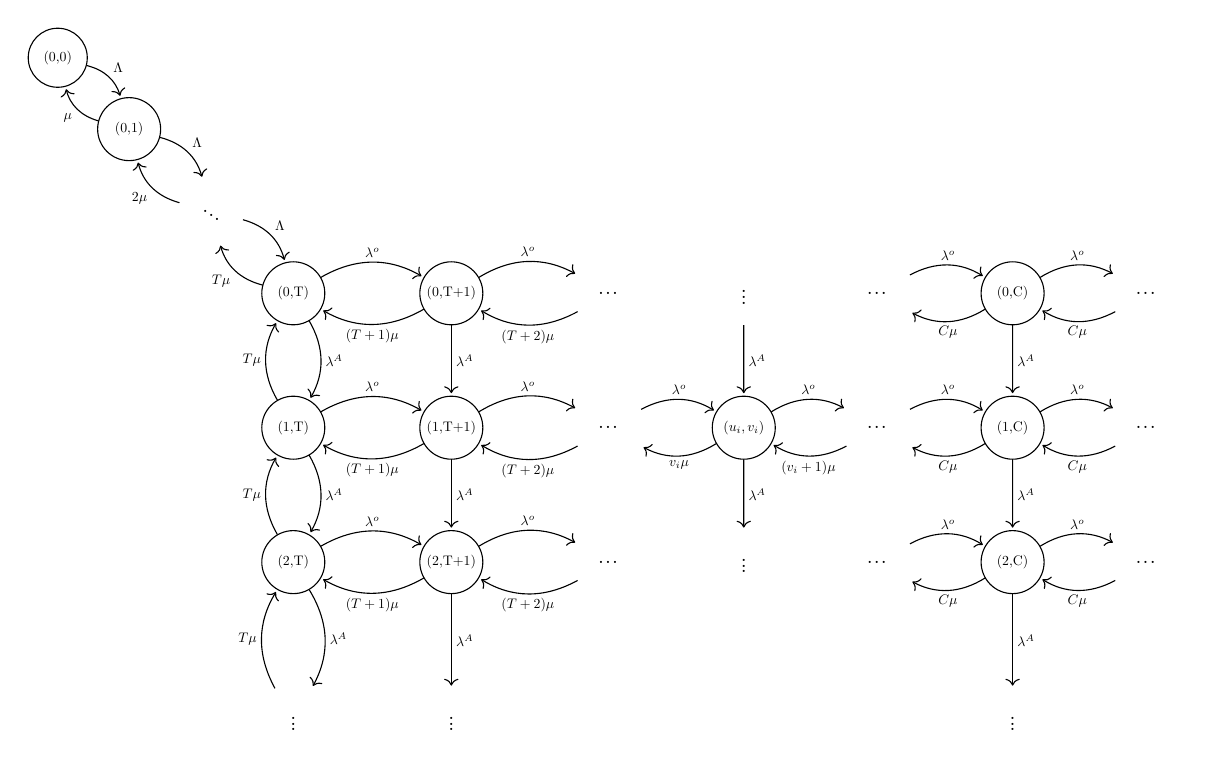
\begin{tikzpicture}[-, node distance = 0.9cm, auto, every node/.style={scale=0.5}]

        % Variables
        \tikzmath{
            let \initdist = 0.5cm;
            let \altdist = 1.2cm;
            let \minsz = 1.6cm;
            let \leftOne = -0.8;
            let \rightOne = 2.2;
            let \upOne = 0.8;
            let \downOne = -2.2;
            let \leftTwo = 2.25;
            let \rightTwo = 14.2;
            let \upTwo = -2.35;
            let \downTwo = -8.8;
        }

        % % Rectangle for S1
        % \draw[ultra thin, dashed] (\leftOne, \downOne) -- (\leftOne, \upOne);
        % \draw[ultra thin, dashed] (\leftOne, \upOne) -- (\rightOne, \upOne);
        % \draw[ultra thin, dashed] (\rightOne, \upOne) -- node {\Huge{\( \quad S_1 \)}}(\rightOne, \downOne);
        % \draw[ultra thin, dashed] (\rightOne, \downOne) -- (\leftOne, \downOne);

        % % Rectangle for S2
        % \draw[ultra thin, dashed] (\leftTwo, \downTwo) -- node {\Huge{\( S_2 \quad \)}}(\leftTwo, \upTwo);
        % \draw[ultra thin, dashed] (\leftTwo, \upTwo) -- (\rightTwo, \upTwo);
        % \draw[ultra thin, dashed] (\rightTwo, \upTwo) -- (\rightTwo, \downTwo);
        % \draw[ultra thin, dashed] (\rightTwo, \downTwo) -- (\leftTwo, \downTwo);

        % First Line
        \node[state, minimum size=1.5cm] (zero) {(0,0)};
        \node[state, node distance = \initdist, minimum size=\minsz, below right=of zero] (one) {(0,1)};
        \node[draw=none, node distance = \initdist, minimum size=\minsz, below right=of one] (two) {\textbf{\( \ddots \)}};
        \node[state, node distance = \initdist, minimum size=\minsz, below right=of two] (three) {(0,T)};
        \node[state, node distance = \altdist, minimum size=\minsz, right=of three] (four) {(0,T+1)};
        \node[draw=none, node distance = \altdist, minimum size=\minsz, right=of four] (five) {\textbf{\dots}};
        \node[draw=none, minimum size=\minsz, right=of five] (six) {\textbf{\vdots}};
        \node[draw=none, minimum size=\minsz, right=of six] (seven) {\textbf{\dots}};
        \node[state, minimum size=\minsz, right=of seven] (eight) {(0,C)};
        \node[draw=none, minimum size=\minsz, right=of eight] (nine) {\textbf{\dots}};


        % Second Line
        \node[state, minimum size=\minsz, below=of three] (three_one) {(1,T)};
        \node[state, minimum size=\minsz, below=of four] (four_one) {(1,T+1)};
        \node[draw=none, minimum size=\minsz, below=of five] (five_one) {\textbf{\dots}};
        \node[state, minimum size=\minsz, right=of five_one] (six_one) {\( (u_i, v_i) \)};
        \node[draw=none, minimum size=\minsz, right=of six_one] (seven_one) {\textbf{\dots}};
        \node[state, minimum size=\minsz, right=of seven_one] (eight_one) {(1,C)};
        \node[draw=none, minimum size=\minsz, right=of eight_one] (nine_one) {\textbf{\dots}};
        

        % Third Line
        \node[state, minimum size=\minsz, below=of three_one] (three_two) {(2,T)};
        \node[state, minimum size=\minsz, below=of four_one] (four_two) {(2,T+1)};
        \node[draw=none, minimum size=\minsz, below=of five_one] (five_two) {\textbf{\dots}};
        \node[draw=none, minimum size=\minsz, right=of five_two] (six_two) {\textbf{\vdots}};
        \node[draw=none, minimum size=\minsz, right=of six_two] (seven_two) {\textbf{\dots}};
        \node[state, minimum size=\minsz, right=of seven_two] (eight_two) {(2,C)};
        \node[draw=none, minimum size=\minsz, right=of eight_two] (nine_two) {\textbf{\dots}};

        % Fourth line
        \node[draw=none, node distance = \altdist, minimum size=\minsz, below=of three_two] (three_three) {\textbf{\vdots}};
        \node[draw=none, node distance = \altdist, minimum size=\minsz, below=of four_two] (four_three) {\textbf{\vdots}};
        \node[draw=none, node distance = \altdist, minimum size=\minsz, below=of five_two] (five_three) {};
        \node[draw=none, node distance = \altdist, minimum size=\minsz, below=of six_two] (six_three) {};
        \node[draw=none, node distance = \altdist, minimum size=\minsz, below=of eight_two] (eight_three) {\textbf{\vdots}};


        \draw[every loop]
            % First Horizontal Edges
            (zero) edge[bend left] node {\( \Lambda \)} (one)
            (one) edge[bend left] node {\( \mu \)} (zero)
            (one) edge[bend left] node {\( \Lambda \)} (two)
            (two) edge[bend left] node {\( 2 \mu \)} (one)
            (two) edge[bend left] node {\( \Lambda \)} (three)
            (three) edge[bend left] node {\( T \mu \)} (two)
            (three) edge[bend left] node {\( \lambda^o \)} (four)
            (four) edge[bend left] node {\( (T+1) \mu \)} (three)
            (four) edge[bend left] node {\( \lambda^o \)} (five)
            (five) edge[bend left] node {\( (T+2) \mu \)} (four)
            % (five) edge[bend left] node {\( \lambda^o \)} (six)
            % (six) edge[bend left] node [above] {\( C\mu \)} (five)
            % (six) edge[bend left] node {\( \lambda^o \)} (seven)
            % (seven) edge[bend left] node [above] {\( C\mu \)} (six)
            (seven) edge[bend left] node {\( \lambda^o \)} (eight)
            (eight) edge[bend left] node {\( C\mu \)} (seven)
            (eight) edge[bend left] node {\( \lambda^o \)} (nine)
            (nine) edge[bend left] node {\( C\mu \)} (eight)

            % Second Horizontal Edges
            (three_one) edge[bend left] node {\( \lambda^o \)} (four_one)
            (four_one) edge[bend left] node {\( (T+1) \mu \)} (three_one)
            (four_one) edge[bend left] node {\( \lambda^o \)} (five_one)
            (five_one) edge[bend left] node {\( (T+2) \mu \)} (four_one)
            (five_one) edge[bend left] node {\( \lambda^o \)} (six_one)
            (six_one) edge[bend left] node {\( v_i\mu \)} (five_one)
            (six_one) edge[bend left] node {\( \lambda^o \)} (seven_one)
            (seven_one) edge[bend left] node {\( (v_i+1)\mu \)} (six_one)
            (seven_one) edge[bend left] node {\( \lambda^o \)} (eight_one)
            (eight_one) edge[bend left] node {\( C\mu \)} (seven_one)
            (eight_one) edge[bend left] node {\( \lambda^o \)} (nine_one)
            (nine_one) edge[bend left] node {\( C\mu \)} (eight_one)

            % Third Horizontal Edges
            (three_two) edge[bend left] node {\( \lambda^o \)} (four_two)
            (four_two) edge[bend left] node [below] {\( (T+1) \mu \)} (three_two)
            (four_two) edge[bend left] node {\( \lambda^o \)} (five_two)
            (five_two) edge[bend left] node {\( (T+2) \mu \)} (four_two)
            % (five_two) edge[bend left] node {\( \lambda^o \)} (six_two)
            % (six_two) edge[bend left] node [above] {\( C\mu \)} (five_two)
            % (six_two) edge[bend left] node {\( \lambda^o \)} (seven_two)
            % (seven_two) edge[bend left] node [above] {\( C\mu \)} (six_two)
            (seven_two) edge[bend left] node {\( \lambda^o \)} (eight_two)
            (eight_two) edge[bend left] node {\( C\mu \)} (seven_two)
            (eight_two) edge[bend left] node {\( \lambda^o \)} (nine_two)
            (nine_two) edge[bend left] node {\( C\mu \)} (eight_two)

            % First Vertical Edges
            (three) edge[bend left] node {\( \lambda^A \)} (three_one)
            (three_one) edge[bend left] node {\( T \mu \)} (three)
            (three_one) edge[bend left] node {\( \lambda^A \)} (three_two)
            (three_two) edge[bend left] node {\( T\mu \)} (three_one)
            (three_two) edge[bend left] node {\( \lambda^A \)} (three_three)
            (three_three) edge[bend left] node {\( T\mu \)} (three_two)

            % Second Vertical Edges
            (four) edge node {\( \lambda^A \)} (four_one)
            (four_one) edge node {\( \lambda^A \)} (four_two)
            (four_two) edge node {\( \lambda^A \)} (four_three)

            % Third Vertical Edges
            (six) edge node {\( \lambda^A \)} (six_one)
            (six_one) edge node {\( \lambda^A \)} (six_two)
            % (six_two) edge node {\( \lambda^A \)} (six_three)

            % Fourth Vertical Edges
            (eight) edge node {\( \lambda^A \)} (eight_one)
            (eight_one) edge node {\( \lambda^A \)} (eight_two)
            (eight_two) edge node {\( \lambda^A \)} (eight_three)
            ;       
    \end{tikzpicture}
    \caption{Markov chains} 
    \label{Markov_4}
\end{figure}




\begin{figure}
    \centering
    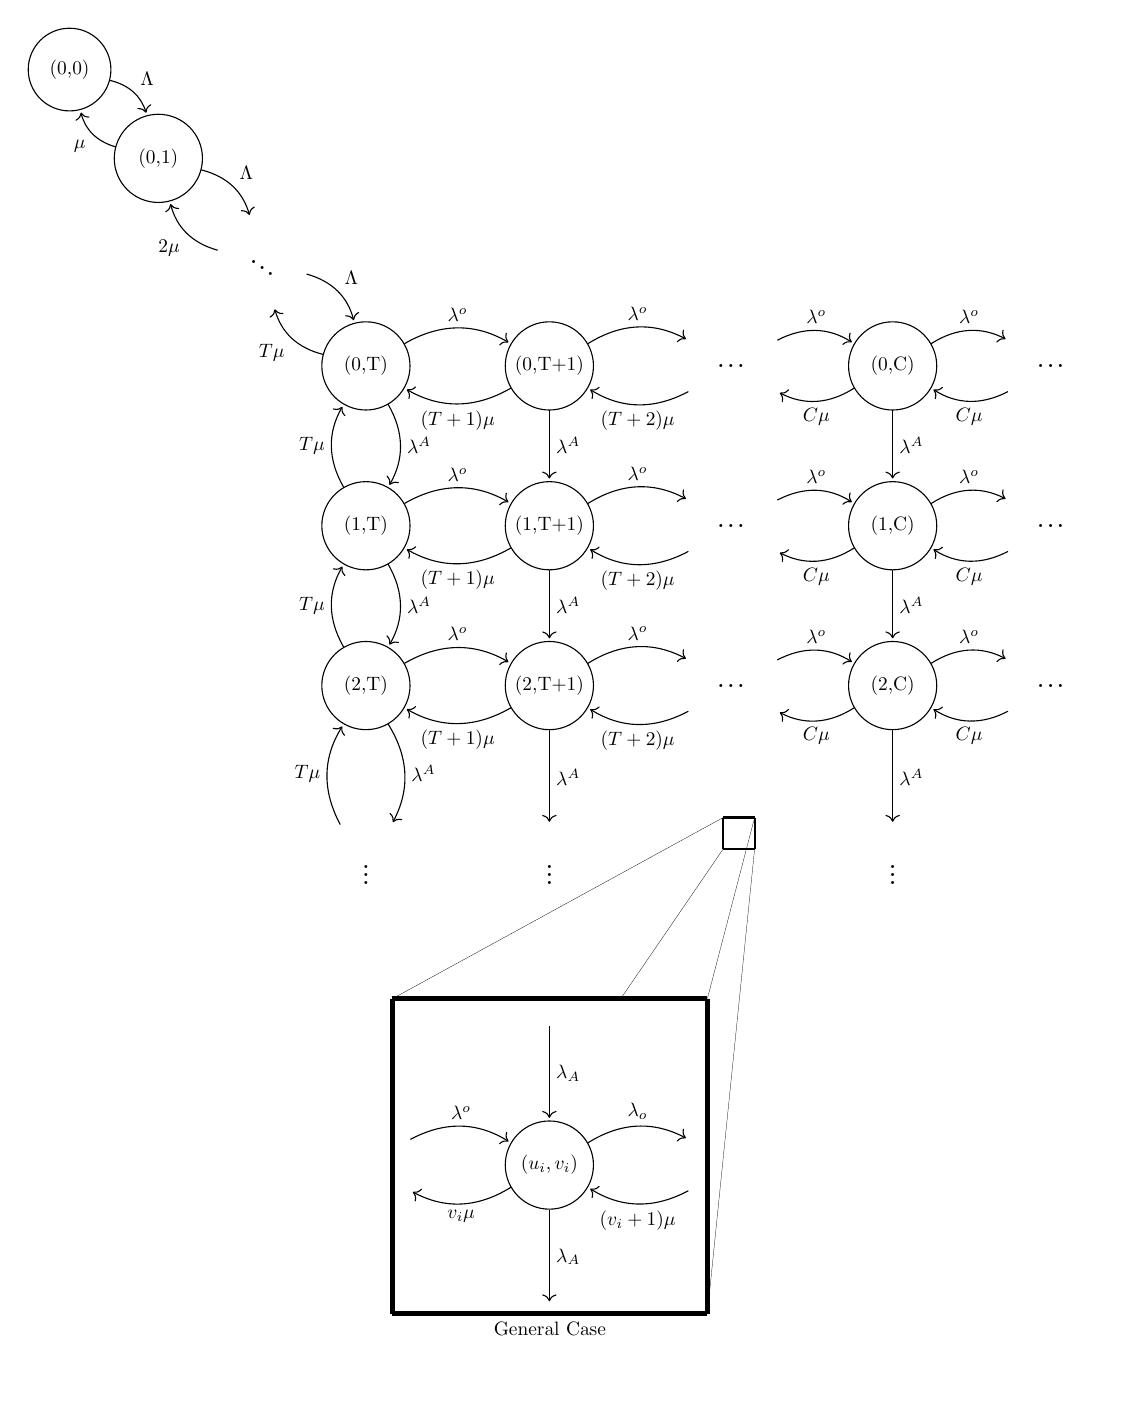
\begin{tikzpicture}[-, node distance = 0.9cm, auto, every node/.style={scale=0.7}]

        % Markov chain variables
        \tikzmath{
            let \initdist = 0.5cm;
            let \altdist = 1.2cm;
            let \minsz = 1.6cm;
        }

        % S_1 and S_2 rectangles
        \tikzmath{
            let \leftOne = -0.8;
            let \rightOne = 2.7;
            let \upOne = 0.8;
            let \downOne = -2.7;
            let \leftTwo = 2.8;
            let \rightTwo = 13;
            let \upTwo = -2.95;
            let \downTwo = -16.4;
        }

        % General case variables
        \tikzmath{
            let \GCsmallx = 8.3;
            let \GCsmally = -9.5;
            let \GCbigx = 4.1;
            let \GCbigy = -11.8;
        }

        % % Rectangle for S1
        % \draw[ultra thin, dashed] (\leftOne, \downOne) -- (\leftOne, \upOne);
        % \draw[ultra thin, dashed] (\leftOne, \upOne) -- (\rightOne, \upOne);
        % \draw[ultra thin, dashed] (\rightOne, \upOne) -- node {\Huge{\( \quad S_1 \)}}(\rightOne, \downOne);
        % \draw[ultra thin, dashed] (\rightOne, \downOne) -- (\leftOne, \downOne);

        % % Rectangle for S2
        % \draw[ultra thin, dashed] (\leftTwo, \downTwo) -- node {\Huge{\( S_2 \quad \)}}(\leftTwo, \upTwo);
        % \draw[ultra thin, dashed] (\leftTwo, \upTwo) -- (\rightTwo, \upTwo);
        % \draw[ultra thin, dashed] (\rightTwo, \upTwo) -- (\rightTwo, \downTwo);
        % \draw[ultra thin, dashed] (\rightTwo, \downTwo) -- (\leftTwo, \downTwo);

        % Small square of general case
        \draw [thick] (\GCsmallx, \GCsmally) -- node {} (\GCsmallx + 0.4, \GCsmally);
        \draw [thick] (\GCsmallx + 0.4, \GCsmally) -- node {} (\GCsmallx + 0.4, \GCsmally - 0.4);
        \draw [thick] (\GCsmallx + 0.4, \GCsmally - 0.4) -- node {} (\GCsmallx, \GCsmally - 0.4);
        \draw [thick] (\GCsmallx, \GCsmally - 0.4) -- node {} (\GCsmallx, \GCsmally);


        % Dashed lines to from small square to big one 
        \draw [ultra thin] (\GCsmallx, \GCsmally) -- node {} (\GCbigx, \GCbigy);
        \draw [ultra thin] (\GCsmallx + 0.4, \GCsmally) -- node {} (\GCbigx + 4, \GCbigy);
        \draw [ultra thin] (\GCsmallx, \GCsmally - 0.4) -- node {} (7, \GCbigy);
        \draw [ultra thin] (\GCsmallx + 0.4, \GCsmally - 0.4) -- node {} (\GCbigx + 4, \GCbigy - 4);
        
        % Big Square of general case
        \draw [ultra thick] (\GCbigx, \GCbigy) -- node {} (\GCbigx + 4, \GCbigy);
        \draw [ultra thick] (\GCbigx + 4, \GCbigy) -- node {} (\GCbigx + 4, \GCbigy - 4);
        \draw [ultra thick] (\GCbigx + 4, \GCbigy - 4) -- node {General Case} (\GCbigx, \GCbigy - 4);
        \draw [ultra thick] (\GCbigx, \GCbigy - 4) -- node {} (\GCbigx, \GCbigy);

        % First Line
        \node[state, minimum size=1.5cm] (zero) {(0,0)};
        \node[state, node distance = \initdist, minimum size=\minsz, below right=of zero] (one) {(0,1)};
        \node[draw=none, node distance = \initdist, minimum size=\minsz, below right=of one] (two) {\textbf{\( \ddots \)}};
        \node[state, node distance = \initdist, minimum size=\minsz, below right=of two] (three) {(0,T)};
        \node[state, node distance = \altdist, minimum size=\minsz, right=of three] (four) {(0,T+1)};
        \node[draw=none, node distance = \altdist, minimum size=\minsz, right=of four] (five) {\textbf{\dots}};
        \node[state, minimum size=\minsz, right=of five] (six) {(0,C)};
        \node[draw=none, minimum size=\minsz, right=of six] (seven) {\textbf{\dots}};

        % Second Line
        \node[state, minimum size=\minsz, below=of three] (three_one) {(1,T)};
        \node[state, minimum size=\minsz, below=of four] (four_one) {(1,T+1)};
        \node[draw=none, minimum size=\minsz, below=of five] (five_one) {\textbf{\dots}};
        \node[state, minimum size=\minsz, right=of five_one] (six_one) {(1,C)};
        \node[draw=none, minimum size=\minsz, right=of six_one] (seven_one) {\textbf{\dots}};
        
        % Third Line
        \node[state, minimum size=\minsz, below=of three_one] (three_two) {(2,T)};
        \node[state, minimum size=\minsz, below=of four_one] (four_two) {(2,T+1)};
        \node[draw=none, minimum size=\minsz, below=of five_one] (five_two) {\textbf{\dots}};
        \node[state, minimum size=\minsz, right=of five_two] (six_two) {(2,C)};
        \node[draw=none, minimum size=\minsz, right=of six_two] (seven_two) {\textbf{\dots}};

        % Fourth line
        \node[draw=none, node distance = \altdist, minimum size=\minsz, below=of three_two] (three_three) {\textbf{\vdots}};
        \node[draw=none, node distance = \altdist, minimum size=\minsz, below=of four_two] (four_three) {\textbf{\vdots}};
        \node[draw=none, node distance = 2cm, minimum size=\minsz, below=of five_two] (five_three) {};
        \node[draw=none, node distance = \altdist, minimum size=\minsz, below=of six_two] (six_three) {\textbf{\vdots}};

        % Fifth line
        % \node[state, node distance = \altdist, minimum size=\minsz, below=of five_three] (general_case_mid) {\( (u_i, v_i) \)};
        \node[draw=none, node distance = 0.3cm, minimum size=\minsz, below=of four_three] (general_case_up) {};
        \node[state, node distance = \altdist, minimum size=\minsz, below=of general_case_up] (general_case_mid) {\( (u_i, v_i) \)};

        \node[draw=none, node distance = \altdist, minimum size=\minsz, below=of general_case_mid] (general_case_down) {};
        \node[draw=none, node distance = \altdist, minimum size=\minsz, left=of general_case_mid] (general_case_left) {};
        \node[draw=none, node distance = \altdist, minimum size=\minsz, right=of general_case_mid] (general_case_right) {};

        \draw[every loop]
            % First Horizontal Edges
            (zero) edge[bend left] node {\( \Lambda \)} (one)
            (one) edge[bend left] node {\( \mu \)} (zero)
            (one) edge[bend left] node {\( \Lambda \)} (two)
            (two) edge[bend left] node {\( 2 \mu \)} (one)
            (two) edge[bend left] node {\( \Lambda \)} (three)
            (three) edge[bend left] node {\( T \mu \)} (two)
            (three) edge[bend left] node {\( \lambda^o \)} (four)
            (four) edge[bend left] node {\( (T+1) \mu \)} (three)
            (four) edge[bend left] node {\( \lambda^o \)} (five)
            (five) edge[bend left] node {\( (T+2) \mu \)} (four)
            (five) edge[bend left] node {\( \lambda^o \)} (six)
            (six) edge[bend left] node {\( C\mu \)} (five)
            (six) edge[bend left] node {\( \lambda^o \)} (seven)
            (seven) edge[bend left] node {\( C\mu \)} (six)

            % Second Horizontal Edges
            (three_one) edge[bend left] node {\( \lambda^o \)} (four_one)
            (four_one) edge[bend left] node {\( (T+1) \mu \)} (three_one)
            (four_one) edge[bend left] node {\( \lambda^o \)} (five_one)
            (five_one) edge[bend left] node {\( (T+2) \mu \)} (four_one)
            (five_one) edge[bend left] node {\( \lambda^o \)} (six_one)
            (six_one) edge[bend left] node {\( C\mu \)} (five_one)
            (six_one) edge[bend left] node {\( \lambda^o \)} (seven_one)
            (seven_one) edge[bend left] node {\( C\mu \)} (six_one)

            % Third Horizontal Edges
            (three_two) edge[bend left] node {\( \lambda^o \)} (four_two)
            (four_two) edge[bend left] node [below] {\( (T+1) \mu \)} (three_two)
            (four_two) edge[bend left] node {\( \lambda^o \)} (five_two)
            (five_two) edge[bend left] node {\( (T+2) \mu \)} (four_two)
            (five_two) edge[bend left] node {\( \lambda^o \)} (six_two)
            (six_two) edge[bend left] node {\( C\mu \)} (five_two)
            (six_two) edge[bend left] node {\( \lambda^o \)} (seven_two)
            (seven_two) edge[bend left] node {\( C\mu \)} (six_two)

            % First Vertical Edges
            (three) edge[bend left] node {\( \lambda^A \)} (three_one)
            (three_one) edge[bend left] node {\( T \mu \)} (three)
            (three_one) edge[bend left] node {\( \lambda^A \)} (three_two)
            (three_two) edge[bend left] node {\( T\mu \)} (three_one)
            (three_two) edge[bend left] node {\( \lambda^A \)} (three_three)
            (three_three) edge[bend left] node {\( T\mu \)} (three_two)

            % Second Vertical Edges
            (four) edge node {\( \lambda^A \)} (four_one)
            (four_one) edge node {\( \lambda^A \)} (four_two)
            (four_two) edge node {\( \lambda^A \)} (four_three)

            % Fourth Vertical Edges
            (six) edge node {\( \lambda^A \)} (six_one)
            (six_one) edge node {\( \lambda^A \)} (six_two)
            (six_two) edge node {\( \lambda^A \)} (six_three)

            % General Case
            (general_case_left) edge[bend left] node {\( \lambda^o \)} (general_case_mid)
            (general_case_mid) edge[bend left] node {\( v_i \mu \)} (general_case_left)
            (general_case_right) edge[bend left] node {\( (v_i +1) \mu \)} (general_case_mid)
            (general_case_mid) edge[bend left] node {\( \lambda_o \)} (general_case_right)
            % (five_three) edge node {\( \lambda_A \)} (general_case_mid)
            (general_case_up) edge node {\( \lambda_A \)} (general_case_mid)
            (general_case_mid) edge node {\( \lambda_A \)} (general_case_down)
            ;
    \end{tikzpicture}
    \caption{Markov chain} 
    \label{Markov_5}
\end{figure}




\newpage
% Quick representation of the steps of methodology
\section{Figures that might be useful}
\begin{figure}[h]
    \centering
    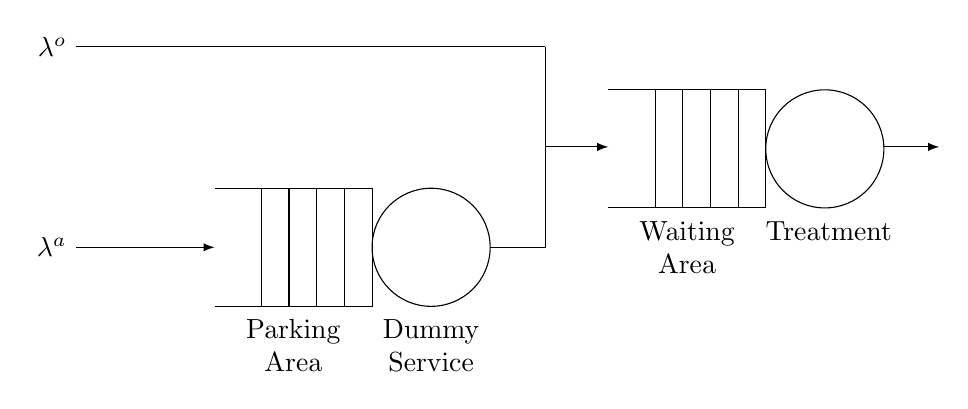
\begin{tikzpicture}[>=latex]
        % the rectangle with vertical rules (Queue 1)
        \draw (0,0) -- ++(2cm,0) -- ++(0,-1.5cm) -- ++(-2cm,0);
        \foreach \i in {1,...,4}
        \draw (2cm-\i*10pt,0) -- +(0,-1.5cm);
        
        % the circle (Queue 1)
        \draw (2.75,-0.75cm) circle [radius=0.75cm];

        % the rectangle with vertical rules (Queue 2)
        \draw (5,1.25) -- ++(2cm,0) -- ++(0,-1.5cm) -- ++(-2cm,0);
        \foreach \i in {1,...,4}
        \draw (7cm-\i*10pt,1.25) -- +(0,-1.5cm);

        % the circle (Queue 2)
        \draw (7.75,0.5) circle [radius=0.75cm];

        % the arrows and labels (Queue 1+2)
        \draw[-] (3.5,-0.75) -- +(20pt,0);
        \draw[<-] (0,-0.75) -- +(-50pt,0) node[left] {\( \lambda^a \)};
        \draw[->] (8.5,0.525) -- +(20pt,0);
        \node[align=center] at (1cm,-2cm) {Parking \\ Area};
        \node[align=center] at (2.75cm,-2cm) {Dummy \\ Service};
        \node[align=center] at (6cm,-0.75cm) {Waiting \\ Area};
        \node[align=center] at (7.8cm,-0.75cm) {Treatment \\ };
        
        \draw (4.2, 1.8) -- +(-169.5pt,0) node[left] {\( \lambda^o \)};
        \draw (4.2, 1.8) -- (4.2, -0.75);
        \draw[->] (4.2, 0.525) -- (5, 0.525);

    \end{tikzpicture}
\end{figure}


\begin{figure}
    \centering
    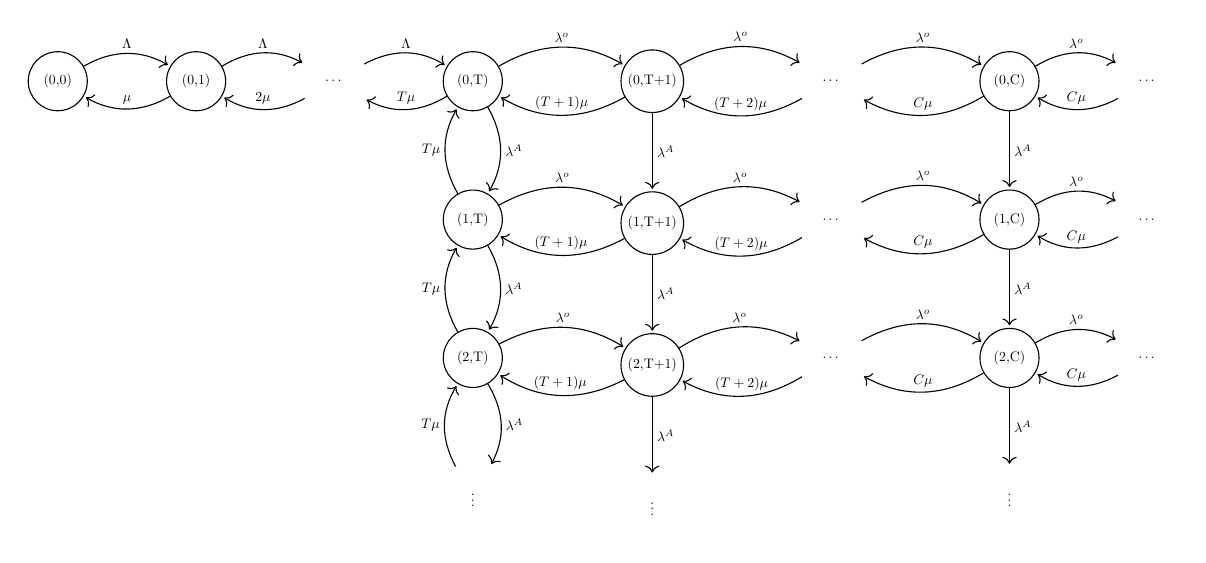
\begin{tikzpicture}[-, node distance = 1cm, auto, every node/.style={scale=0.5}]

        % Variables
        \tikzmath{
            let \altdist = 1.5cm;
            let \minsz = 1.5cm;
        }

        % First Line
        \node[state, minimum size=1.5cm] (zero) {(0,0)};
        \node[state, minimum size=1.5cm,  right=of zero] (one) {(0,1)};
        \node[draw=none, minimum size=1.5cm, right=of one] (two) {\dots};
        \node[state, minimum size=1.5cm, right=of two] (three) {(0,T)};
        \node[state, node distance = \altdist, minimum size=\minsz, right=of three] (four) {(0,T+1)};
        \node[draw=none, node distance = \altdist, minimum size=\minsz, right=of four] (five) {\dots};
        \node[state, node distance = \altdist, minimum size=\minsz, right=of five] (six) {(0,C)};
        \node[draw=none, minimum size=\minsz, right=of six] (seven) {\dots};

        % Second Line
        \node[state, minimum size=\minsz, below=of three] (three_one) {(1,T)};
        \node[state, minimum size=\minsz, below=of four] (four_one) {(1,T+1)};
        \node[draw=none, minimum size=\minsz, below=of five] (five_one) {\dots};
        \node[state, node distance = \altdist, minimum size=\minsz, right=of five_one] (six_one) {(1,C)};
        \node[draw=none, minimum size=\minsz, right=of six_one] (seven_one) {\dots};

        % Third Line
        \node[state, minimum size=\minsz, below=of three_one] (three_two) {(2,T)};
        \node[state, minimum size=\minsz, below=of four_one] (four_two) {(2,T+1)};
        \node[draw=none, minimum size=\minsz, below=of five_one] (five_two) {\dots};
        \node[state, node distance = \altdist, minimum size=\minsz, right=of five_two] (six_two) {(2,C)};
        \node[draw=none, minimum size=\minsz, right=of six_two] (seven_two) {\dots};

        % Fourth line
        \node[draw=none, minimum size=\minsz, below=of three_two] (three_three) {\vdots};
        \node[draw=none, minimum size=\minsz, below=of four_two] (four_three) {\vdots};
        \node[draw=none, minimum size=\minsz, below=of five_two] (five_three) {};
        \node[draw=none, node distance = \altdist, minimum size=\minsz, right=of five_three] (six_three) {\vdots};

        \draw[every loop]
            % First Horizontal Edges
            (zero) edge[bend left] node {\( \Lambda \)} (one)
            (one) edge[bend left] node [above] {\( \mu \)} (zero)
            (one) edge[bend left] node {\( \Lambda \)} (two)
            (two) edge[bend left] node [above] {\( 2 \mu \)} (one)
            (two) edge[bend left] node {\( \Lambda \)} (three)
            (three) edge[bend left] node [above] {\( T \mu \)} (two)
            (three) edge[bend left] node {\( \lambda^o \)} (four)
            (four) edge[bend left] node [above] {\( (T+1) \mu \)} (three)
            (four) edge[bend left] node {\( \lambda^o \)} (five)
            (five) edge[bend left] node [above] {\( (T+2) \mu \)} (four)
            (five) edge[bend left] node {\( \lambda^o \)} (six)
            (six) edge[bend left] node [above] {\( C\mu \)} (five)
            (six) edge[bend left] node {\( \lambda^o \)} (seven)
            (seven) edge[bend left] node [above] {\( C\mu \)} (six)

            % Second Horizontal Edges
            (three_one) edge[bend left] node {\( \lambda^o \)} (four_one)
            (four_one) edge[bend left] node [above] {\( (T+1) \mu \)} (three_one)
            (four_one) edge[bend left] node {\( \lambda^o \)} (five_one)
            (five_one) edge[bend left] node [above] {\( (T+2) \mu \)} (four_one)
            (five_one) edge[bend left] node {\( \lambda^o \)} (six_one)
            (six_one) edge[bend left] node [above] {\( C\mu \)} (five_one)
            (six_one) edge[bend left] node {\( \lambda^o \)} (seven_one)
            (seven_one) edge[bend left] node [above] {\( C\mu \)} (six_one)

            % Third Horizontal Edges
            (three_two) edge[bend left] node {\( \lambda^o \)} (four_two)
            (four_two) edge[bend left] node [above] {\( (T+1) \mu \)} (three_two)
            (four_two) edge[bend left] node {\( \lambda^o \)} (five_two)
            (five_two) edge[bend left] node [above] {\( (T+2) \mu \)} (four_two)
            (five_two) edge[bend left] node {\( \lambda^o \)} (six_two)
            (six_two) edge[bend left] node [above] {\( C\mu \)} (five_two)
            (six_two) edge[bend left] node {\( \lambda^o \)} (seven_two)
            (seven_two) edge[bend left] node [above] {\( C\mu \)} (six_two)

            % First Vertical Edges
            (three) edge[bend left] node {\( \lambda^A \)} (three_one)
            (three_one) edge[bend left] node {\( T \mu \)} (three)
            (three_one) edge[bend left] node {\( \lambda^A \)} (three_two)
            (three_two) edge[bend left] node {\( T\mu \)} (three_one)
            (three_two) edge[bend left] node {\( \lambda^A \)} (three_three)
            (three_three) edge[bend left] node {\( T\mu \)} (three_two)

            % Second Vertical Edges
            (four) edge node {\( \lambda^A \)} (four_one)
            (four_one) edge node {\( \lambda^A \)} (four_two)
            (four_two) edge node {\( \lambda^A \)} (four_three)

            %Third Vertical Edges
            (six) edge node {\( \lambda^A \)} (six_one)
            (six_one) edge node {\( \lambda^A \)} (six_two)
            (six_two) edge node {\( \lambda^A \)} (six_three)
            ;       
    \end{tikzpicture}
    \caption{Markov chains} 
    \label{Markov_2}
\end{figure}



\begin{figure}
    \centering
    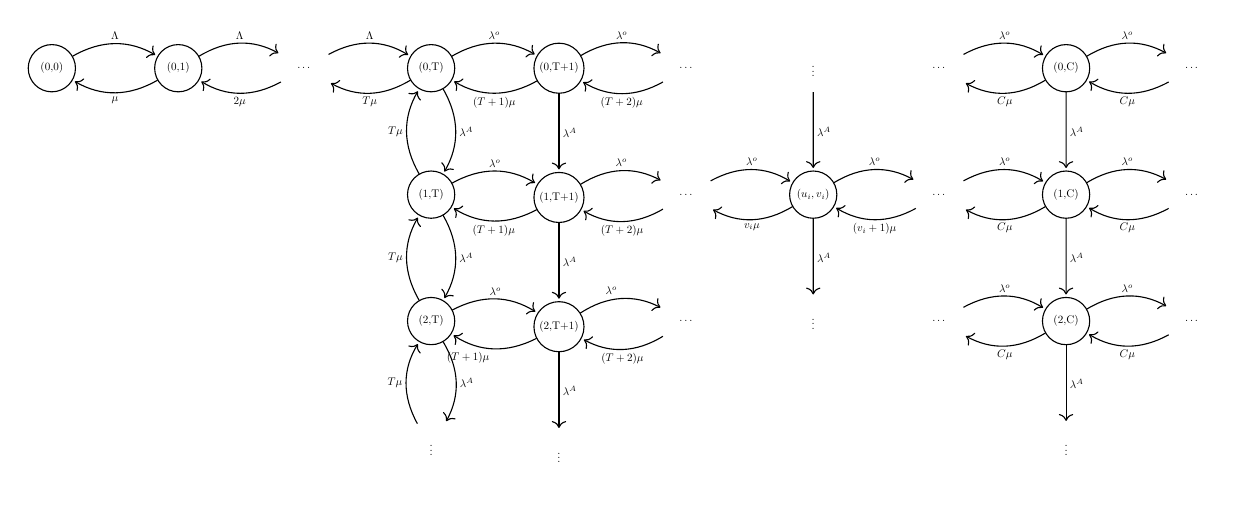
\begin{tikzpicture}[-, node distance = 1cm, auto, every node/.style={scale=0.4}]

        % Variables
        \tikzmath{
            let \altdist = 1cm;
            let \minsz = 1.5cm;
        }

        % First Line
        \node[state, minimum size=1.5cm] (zero) {(0,0)};
        \node[state, minimum size=1.5cm,  right=of zero] (one) {(0,1)};
        \node[draw=none, minimum size=1.5cm, right=of one] (two) {\dots};
        \node[state, minimum size=1.5cm, right=of two] (three) {(0,T)};
        \node[state, node distance = \altdist, minimum size=\minsz, right=of three] (four) {(0,T+1)};
        \node[draw=none, minimum size=\minsz, right=of four] (five) {\dots};
        \node[draw=none, minimum size=\minsz, right=of five] (six) {\vdots};
        \node[draw=none, minimum size=\minsz, right=of six] (seven) {\dots};
        \node[state, minimum size=\minsz, right=of seven] (eight) {(0,C)};
        \node[draw=none, minimum size=\minsz, right=of eight] (nine) {\dots};


        % Second Line
        \node[state, minimum size=\minsz, below=of three] (three_one) {(1,T)};
        \node[state, minimum size=\minsz, below=of four] (four_one) {(1,T+1)};
        \node[draw=none, minimum size=\minsz, below=of five] (five_one) {\dots};
        \node[state, node distance = \altdist, minimum size=\minsz, right=of five_one] (six_one) {\( (u_i, v_i) \)};
        \node[draw=none, minimum size=\minsz, right=of six_one] (seven_one) {\dots};
        \node[state, node distance = \altdist, minimum size=\minsz, right=of seven_one] (eight_one) {(1,C)};
        \node[draw=none, minimum size=\minsz, right=of eight_one] (nine_one) {\dots};
        

        % Third Line
        \node[state, minimum size=\minsz, below=of three_one] (three_two) {(2,T)};
        \node[state, minimum size=\minsz, below=of four_one] (four_two) {(2,T+1)};
        \node[draw=none, minimum size=\minsz, below=of five_one] (five_two) {\dots};
        \node[draw=none, node distance = \altdist, minimum size=\minsz, right=of five_two] (six_two) {\vdots};
        \node[draw=none, minimum size=\minsz, right=of six_two] (seven_two) {\dots};
        \node[state, node distance = \altdist, minimum size=\minsz, right=of seven_two] (eight_two) {(2,C)};
        \node[draw=none, minimum size=\minsz, right=of eight_two] (nine_two) {\dots};

        % Fourth line
        \node[draw=none, minimum size=\minsz, below=of three_two] (three_three) {\vdots};
        \node[draw=none, minimum size=\minsz, below=of four_two] (four_three) {\vdots};
        \node[draw=none, minimum size=\minsz, below=of five_two] (five_three) {};
        \node[draw=none, node distance = \altdist, minimum size=\minsz, right=of five_three] (six_three) {};
        \node[draw=none, node distance = \altdist, minimum size=\minsz, below=of eight_two] (eight_three) {\vdots};


        \draw[every loop]
            % First Horizontal Edges
            (zero) edge[bend left] node {\( \Lambda \)} (one)
            (one) edge[bend left] node {\( \mu \)} (zero)
            (one) edge[bend left] node {\( \Lambda \)} (two)
            (two) edge[bend left] node {\( 2 \mu \)} (one)
            (two) edge[bend left] node {\( \Lambda \)} (three)
            (three) edge[bend left] node {\( T \mu \)} (two)
            (three) edge[bend left] node {\( \lambda^o \)} (four)
            (four) edge[bend left] node {\( (T+1) \mu \)} (three)
            (four) edge[bend left] node {\( \lambda^o \)} (five)
            (five) edge[bend left] node {\( (T+2) \mu \)} (four)
            % (five) edge[bend left] node {\( \lambda^o \)} (six)
            % (six) edge[bend left] node [above] {\( C\mu \)} (five)
            % (six) edge[bend left] node {\( \lambda^o \)} (seven)
            % (seven) edge[bend left] node [above] {\( C\mu \)} (six)
            (seven) edge[bend left] node {\( \lambda^o \)} (eight)
            (eight) edge[bend left] node {\( C\mu \)} (seven)
            (eight) edge[bend left] node {\( \lambda^o \)} (nine)
            (nine) edge[bend left] node {\( C\mu \)} (eight)

            % Second Horizontal Edges
            (three_one) edge[bend left] node {\(\lambda^o\)} (four_one)
            (four_one) edge[bend left] node {\( (T+1) \mu \)} (three_one)
            (four_one) edge[bend left] node {\( \lambda^o \)} (five_one)
            (five_one) edge[bend left] node {\( (T+2) \mu \)} (four_one)
            (five_one) edge[bend left] node {\( \lambda^o \)} (six_one)
            (six_one) edge[bend left] node {\( v_i\mu \)} (five_one)
            (six_one) edge[bend left] node {\( \lambda^o \)} (seven_one)
            (seven_one) edge[bend left] node {\( (v_i+1)\mu \)} (six_one)
            (seven_one) edge[bend left] node {\( \lambda^o \)} (eight_one)
            (eight_one) edge[bend left] node {\( C\mu \)} (seven_one)
            (eight_one) edge[bend left] node {\( \lambda^o \)} (nine_one)
            (nine_one) edge[bend left] node {\( C\mu \)} (eight_one)

            % Third Horizontal Edges
            (three_two) edge[bend left] node {\( \lambda^o \)} (four_two)
            (four_two) edge[bend left] node {\( (T+1) \mu \)} (three_two)
            (four_two) edge[bend left] node {\( \lambda^o \)} (five_two)
            (five_two) edge[bend left] node {\( (T+2) \mu \)} (four_two)
            % (five_two) edge[bend left] node {\( \lambda^o \)} (six_two)
            % (six_two) edge[bend left] node [above] {\( C\mu \)} (five_two)
            % (six_two) edge[bend left] node {\( \lambda^o \)} (seven_two)
            % (seven_two) edge[bend left] node [above] {\( C\mu \)} (six_two)
            (seven_two) edge[bend left] node {\( \lambda^o \)} (eight_two)
            (eight_two) edge[bend left] node {\( C\mu \)} (seven_two)
            (eight_two) edge[bend left] node {\( \lambda^o \)} (nine_two)
            (nine_two) edge[bend left] node {\( C\mu \)} (eight_two)

            % First Vertical Edges
            (three) edge[bend left] node {\( \lambda^A \)} (three_one)
            (three_one) edge[bend left] node {\( T \mu \)} (three)
            (three_one) edge[bend left] node {\( \lambda^A \)} (three_two)
            (three_two) edge[bend left] node {\( T\mu \)} (three_one)
            (three_two) edge[bend left] node {\( \lambda^A \)} (three_three)
            (three_three) edge[bend left] node {\( T\mu \)} (three_two)

            % Second Vertical Edges
            (four) edge node {\( \lambda^A \)} (four_one)
            (four_one) edge node {\( \lambda^A \)} (four_two)
            (four_two) edge node {\( \lambda^A \)} (four_three)

            % Third Vertical Edges
            (six) edge node {\( \lambda^A \)} (six_one)
            (six_one) edge node {\( \lambda^A \)} (six_two)
            % (six_two) edge node {\( \lambda^A \)} (six_three)

            % Fourth Vertical Edges
            (eight) edge node {\( \lambda^A \)} (eight_one)
            (eight_one) edge node {\( \lambda^A \)} (eight_two)
            (eight_two) edge node {\( \lambda^A \)} (eight_three)
            ;       
    \end{tikzpicture}
    \caption{Markov chains} 
    \label{Markov_3}
\end{figure}


\begin{figure}
    \centering
    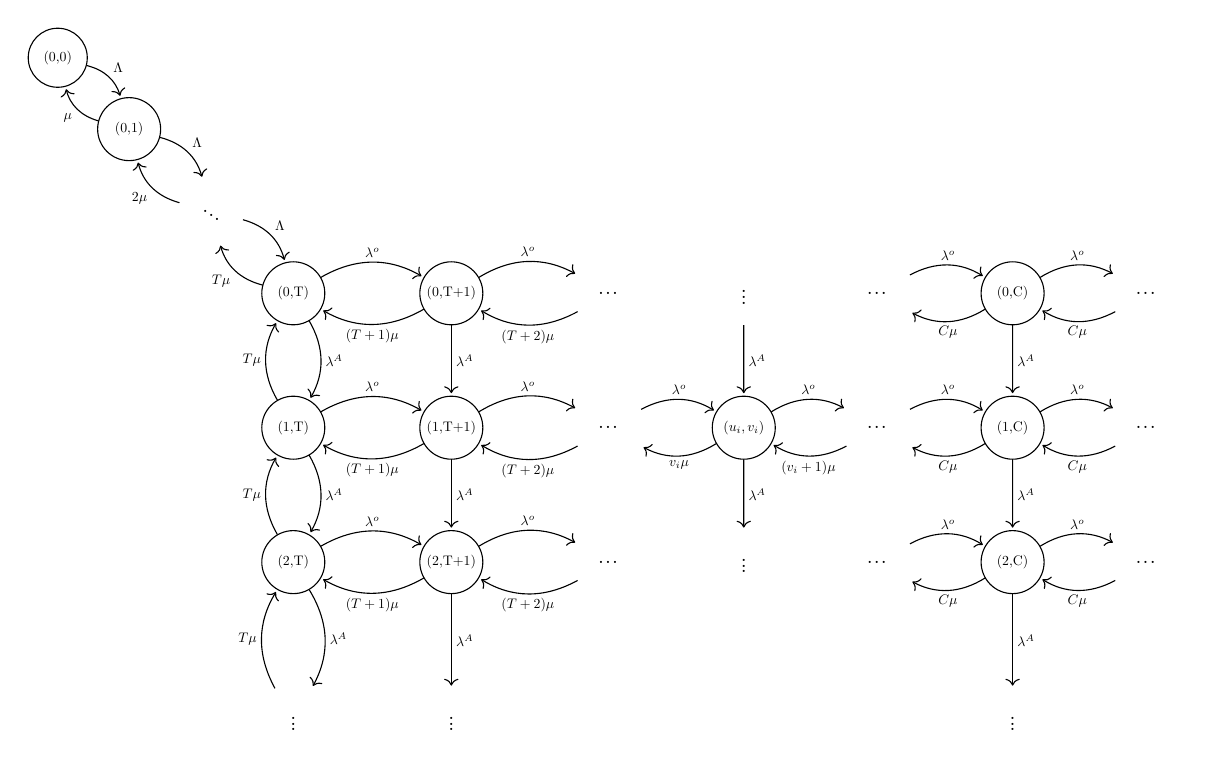
\begin{tikzpicture}[-, node distance = 0.9cm, auto, every node/.style={scale=0.5}]

        % Variables
        \tikzmath{
            let \initdist = 0.5cm;
            let \altdist = 1.2cm;
            let \minsz = 1.6cm;
            let \leftOne = -0.8;
            let \rightOne = 2.2;
            let \upOne = 0.8;
            let \downOne = -2.2;
            let \leftTwo = 2.25;
            let \rightTwo = 14.2;
            let \upTwo = -2.35;
            let \downTwo = -8.8;
        }

        % % Rectangle for S1
        % \draw[ultra thin, dashed] (\leftOne, \downOne) -- (\leftOne, \upOne);
        % \draw[ultra thin, dashed] (\leftOne, \upOne) -- (\rightOne, \upOne);
        % \draw[ultra thin, dashed] (\rightOne, \upOne) -- node {\Huge{\( \quad S_1 \)}}(\rightOne, \downOne);
        % \draw[ultra thin, dashed] (\rightOne, \downOne) -- (\leftOne, \downOne);

        % % Rectangle for S2
        % \draw[ultra thin, dashed] (\leftTwo, \downTwo) -- node {\Huge{\( S_2 \quad \)}}(\leftTwo, \upTwo);
        % \draw[ultra thin, dashed] (\leftTwo, \upTwo) -- (\rightTwo, \upTwo);
        % \draw[ultra thin, dashed] (\rightTwo, \upTwo) -- (\rightTwo, \downTwo);
        % \draw[ultra thin, dashed] (\rightTwo, \downTwo) -- (\leftTwo, \downTwo);

        % First Line
        \node[state, minimum size=1.5cm] (zero) {(0,0)};
        \node[state, node distance = \initdist, minimum size=\minsz, below right=of zero] (one) {(0,1)};
        \node[draw=none, node distance = \initdist, minimum size=\minsz, below right=of one] (two) {\textbf{\( \ddots \)}};
        \node[state, node distance = \initdist, minimum size=\minsz, below right=of two] (three) {(0,T)};
        \node[state, node distance = \altdist, minimum size=\minsz, right=of three] (four) {(0,T+1)};
        \node[draw=none, node distance = \altdist, minimum size=\minsz, right=of four] (five) {\textbf{\dots}};
        \node[draw=none, minimum size=\minsz, right=of five] (six) {\textbf{\vdots}};
        \node[draw=none, minimum size=\minsz, right=of six] (seven) {\textbf{\dots}};
        \node[state, minimum size=\minsz, right=of seven] (eight) {(0,C)};
        \node[draw=none, minimum size=\minsz, right=of eight] (nine) {\textbf{\dots}};


        % Second Line
        \node[state, minimum size=\minsz, below=of three] (three_one) {(1,T)};
        \node[state, minimum size=\minsz, below=of four] (four_one) {(1,T+1)};
        \node[draw=none, minimum size=\minsz, below=of five] (five_one) {\textbf{\dots}};
        \node[state, minimum size=\minsz, right=of five_one] (six_one) {\( (u_i, v_i) \)};
        \node[draw=none, minimum size=\minsz, right=of six_one] (seven_one) {\textbf{\dots}};
        \node[state, minimum size=\minsz, right=of seven_one] (eight_one) {(1,C)};
        \node[draw=none, minimum size=\minsz, right=of eight_one] (nine_one) {\textbf{\dots}};
        

        % Third Line
        \node[state, minimum size=\minsz, below=of three_one] (three_two) {(2,T)};
        \node[state, minimum size=\minsz, below=of four_one] (four_two) {(2,T+1)};
        \node[draw=none, minimum size=\minsz, below=of five_one] (five_two) {\textbf{\dots}};
        \node[draw=none, minimum size=\minsz, right=of five_two] (six_two) {\textbf{\vdots}};
        \node[draw=none, minimum size=\minsz, right=of six_two] (seven_two) {\textbf{\dots}};
        \node[state, minimum size=\minsz, right=of seven_two] (eight_two) {(2,C)};
        \node[draw=none, minimum size=\minsz, right=of eight_two] (nine_two) {\textbf{\dots}};

        % Fourth line
        \node[draw=none, node distance = \altdist, minimum size=\minsz, below=of three_two] (three_three) {\textbf{\vdots}};
        \node[draw=none, node distance = \altdist, minimum size=\minsz, below=of four_two] (four_three) {\textbf{\vdots}};
        \node[draw=none, node distance = \altdist, minimum size=\minsz, below=of five_two] (five_three) {};
        \node[draw=none, node distance = \altdist, minimum size=\minsz, below=of six_two] (six_three) {};
        \node[draw=none, node distance = \altdist, minimum size=\minsz, below=of eight_two] (eight_three) {\textbf{\vdots}};


        \draw[every loop]
            % First Horizontal Edges
            (zero) edge[bend left] node {\( \Lambda \)} (one)
            (one) edge[bend left] node {\( \mu \)} (zero)
            (one) edge[bend left] node {\( \Lambda \)} (two)
            (two) edge[bend left] node {\( 2 \mu \)} (one)
            (two) edge[bend left] node {\( \Lambda \)} (three)
            (three) edge[bend left] node {\( T \mu \)} (two)
            (three) edge[bend left] node {\( \lambda^o \)} (four)
            (four) edge[bend left] node {\( (T+1) \mu \)} (three)
            (four) edge[bend left] node {\( \lambda^o \)} (five)
            (five) edge[bend left] node {\( (T+2) \mu \)} (four)
            % (five) edge[bend left] node {\( \lambda^o \)} (six)
            % (six) edge[bend left] node [above] {\( C\mu \)} (five)
            % (six) edge[bend left] node {\( \lambda^o \)} (seven)
            % (seven) edge[bend left] node [above] {\( C\mu \)} (six)
            (seven) edge[bend left] node {\( \lambda^o \)} (eight)
            (eight) edge[bend left] node {\( C\mu \)} (seven)
            (eight) edge[bend left] node {\( \lambda^o \)} (nine)
            (nine) edge[bend left] node {\( C\mu \)} (eight)

            % Second Horizontal Edges
            (three_one) edge[bend left] node {\( \lambda^o \)} (four_one)
            (four_one) edge[bend left] node {\( (T+1) \mu \)} (three_one)
            (four_one) edge[bend left] node {\( \lambda^o \)} (five_one)
            (five_one) edge[bend left] node {\( (T+2) \mu \)} (four_one)
            (five_one) edge[bend left] node {\( \lambda^o \)} (six_one)
            (six_one) edge[bend left] node {\( v_i\mu \)} (five_one)
            (six_one) edge[bend left] node {\( \lambda^o \)} (seven_one)
            (seven_one) edge[bend left] node {\( (v_i+1)\mu \)} (six_one)
            (seven_one) edge[bend left] node {\( \lambda^o \)} (eight_one)
            (eight_one) edge[bend left] node {\( C\mu \)} (seven_one)
            (eight_one) edge[bend left] node {\( \lambda^o \)} (nine_one)
            (nine_one) edge[bend left] node {\( C\mu \)} (eight_one)

            % Third Horizontal Edges
            (three_two) edge[bend left] node {\( \lambda^o \)} (four_two)
            (four_two) edge[bend left] node [below] {\( (T+1) \mu \)} (three_two)
            (four_two) edge[bend left] node {\( \lambda^o \)} (five_two)
            (five_two) edge[bend left] node {\( (T+2) \mu \)} (four_two)
            % (five_two) edge[bend left] node {\( \lambda^o \)} (six_two)
            % (six_two) edge[bend left] node [above] {\( C\mu \)} (five_two)
            % (six_two) edge[bend left] node {\( \lambda^o \)} (seven_two)
            % (seven_two) edge[bend left] node [above] {\( C\mu \)} (six_two)
            (seven_two) edge[bend left] node {\( \lambda^o \)} (eight_two)
            (eight_two) edge[bend left] node {\( C\mu \)} (seven_two)
            (eight_two) edge[bend left] node {\( \lambda^o \)} (nine_two)
            (nine_two) edge[bend left] node {\( C\mu \)} (eight_two)

            % First Vertical Edges
            (three) edge[bend left] node {\( \lambda^A \)} (three_one)
            (three_one) edge[bend left] node {\( T \mu \)} (three)
            (three_one) edge[bend left] node {\( \lambda^A \)} (three_two)
            (three_two) edge[bend left] node {\( T\mu \)} (three_one)
            (three_two) edge[bend left] node {\( \lambda^A \)} (three_three)
            (three_three) edge[bend left] node {\( T\mu \)} (three_two)

            % Second Vertical Edges
            (four) edge node {\( \lambda^A \)} (four_one)
            (four_one) edge node {\( \lambda^A \)} (four_two)
            (four_two) edge node {\( \lambda^A \)} (four_three)

            % Third Vertical Edges
            (six) edge node {\( \lambda^A \)} (six_one)
            (six_one) edge node {\( \lambda^A \)} (six_two)
            % (six_two) edge node {\( \lambda^A \)} (six_three)

            % Fourth Vertical Edges
            (eight) edge node {\( \lambda^A \)} (eight_one)
            (eight_one) edge node {\( \lambda^A \)} (eight_two)
            (eight_two) edge node {\( \lambda^A \)} (eight_three)
            ;       
    \end{tikzpicture}
    \caption{Markov chains} 
    \label{Markov_4}
\end{figure}




\begin{figure}
    \centering
    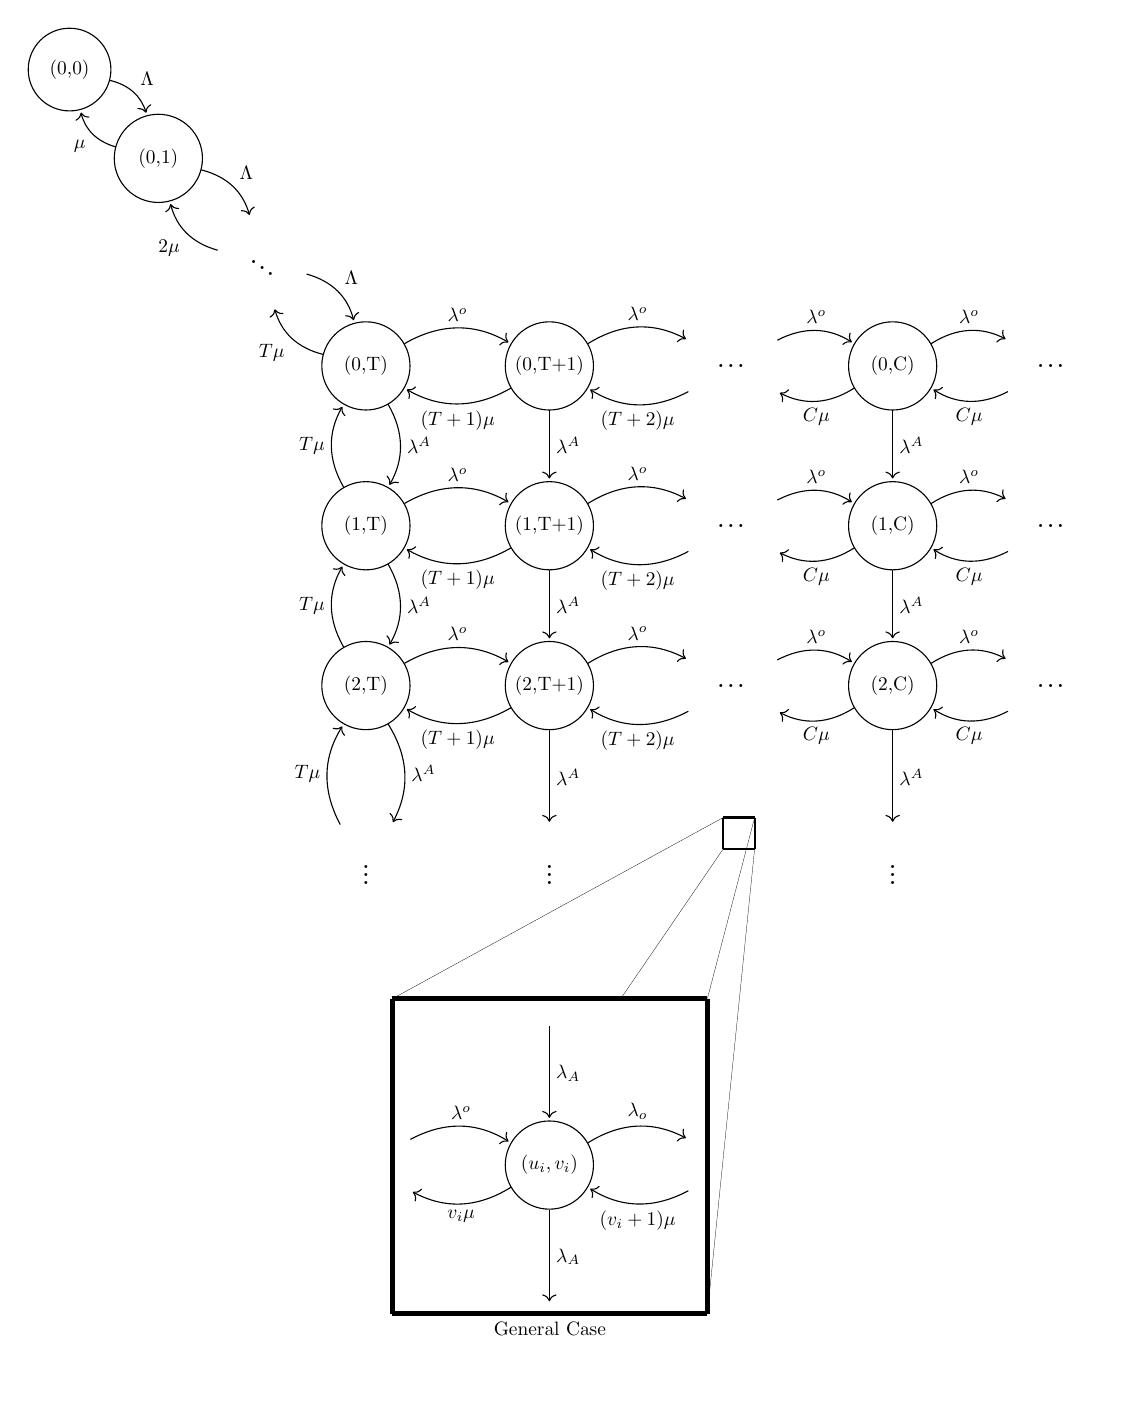
\begin{tikzpicture}[-, node distance = 0.9cm, auto, every node/.style={scale=0.7}]

        % Markov chain variables
        \tikzmath{
            let \initdist = 0.5cm;
            let \altdist = 1.2cm;
            let \minsz = 1.6cm;
        }

        % S_1 and S_2 rectangles
        \tikzmath{
            let \leftOne = -0.8;
            let \rightOne = 2.7;
            let \upOne = 0.8;
            let \downOne = -2.7;
            let \leftTwo = 2.8;
            let \rightTwo = 13;
            let \upTwo = -2.95;
            let \downTwo = -16.4;
        }

        % General case variables
        \tikzmath{
            let \GCsmallx = 8.3;
            let \GCsmally = -9.5;
            let \GCbigx = 4.1;
            let \GCbigy = -11.8;
        }

        % % Rectangle for S1
        % \draw[ultra thin, dashed] (\leftOne, \downOne) -- (\leftOne, \upOne);
        % \draw[ultra thin, dashed] (\leftOne, \upOne) -- (\rightOne, \upOne);
        % \draw[ultra thin, dashed] (\rightOne, \upOne) -- node {\Huge{\( \quad S_1 \)}}(\rightOne, \downOne);
        % \draw[ultra thin, dashed] (\rightOne, \downOne) -- (\leftOne, \downOne);

        % % Rectangle for S2
        % \draw[ultra thin, dashed] (\leftTwo, \downTwo) -- node {\Huge{\( S_2 \quad \)}}(\leftTwo, \upTwo);
        % \draw[ultra thin, dashed] (\leftTwo, \upTwo) -- (\rightTwo, \upTwo);
        % \draw[ultra thin, dashed] (\rightTwo, \upTwo) -- (\rightTwo, \downTwo);
        % \draw[ultra thin, dashed] (\rightTwo, \downTwo) -- (\leftTwo, \downTwo);

        % Small square of general case
        \draw [thick] (\GCsmallx, \GCsmally) -- node {} (\GCsmallx + 0.4, \GCsmally);
        \draw [thick] (\GCsmallx + 0.4, \GCsmally) -- node {} (\GCsmallx + 0.4, \GCsmally - 0.4);
        \draw [thick] (\GCsmallx + 0.4, \GCsmally - 0.4) -- node {} (\GCsmallx, \GCsmally - 0.4);
        \draw [thick] (\GCsmallx, \GCsmally - 0.4) -- node {} (\GCsmallx, \GCsmally);


        % Dashed lines to from small square to big one 
        \draw [ultra thin] (\GCsmallx, \GCsmally) -- node {} (\GCbigx, \GCbigy);
        \draw [ultra thin] (\GCsmallx + 0.4, \GCsmally) -- node {} (\GCbigx + 4, \GCbigy);
        \draw [ultra thin] (\GCsmallx, \GCsmally - 0.4) -- node {} (7, \GCbigy);
        \draw [ultra thin] (\GCsmallx + 0.4, \GCsmally - 0.4) -- node {} (\GCbigx + 4, \GCbigy - 4);
        
        % Big Square of general case
        \draw [ultra thick] (\GCbigx, \GCbigy) -- node {} (\GCbigx + 4, \GCbigy);
        \draw [ultra thick] (\GCbigx + 4, \GCbigy) -- node {} (\GCbigx + 4, \GCbigy - 4);
        \draw [ultra thick] (\GCbigx + 4, \GCbigy - 4) -- node {General Case} (\GCbigx, \GCbigy - 4);
        \draw [ultra thick] (\GCbigx, \GCbigy - 4) -- node {} (\GCbigx, \GCbigy);

        % First Line
        \node[state, minimum size=1.5cm] (zero) {(0,0)};
        \node[state, node distance = \initdist, minimum size=\minsz, below right=of zero] (one) {(0,1)};
        \node[draw=none, node distance = \initdist, minimum size=\minsz, below right=of one] (two) {\textbf{\( \ddots \)}};
        \node[state, node distance = \initdist, minimum size=\minsz, below right=of two] (three) {(0,T)};
        \node[state, node distance = \altdist, minimum size=\minsz, right=of three] (four) {(0,T+1)};
        \node[draw=none, node distance = \altdist, minimum size=\minsz, right=of four] (five) {\textbf{\dots}};
        \node[state, minimum size=\minsz, right=of five] (six) {(0,C)};
        \node[draw=none, minimum size=\minsz, right=of six] (seven) {\textbf{\dots}};

        % Second Line
        \node[state, minimum size=\minsz, below=of three] (three_one) {(1,T)};
        \node[state, minimum size=\minsz, below=of four] (four_one) {(1,T+1)};
        \node[draw=none, minimum size=\minsz, below=of five] (five_one) {\textbf{\dots}};
        \node[state, minimum size=\minsz, right=of five_one] (six_one) {(1,C)};
        \node[draw=none, minimum size=\minsz, right=of six_one] (seven_one) {\textbf{\dots}};
        
        % Third Line
        \node[state, minimum size=\minsz, below=of three_one] (three_two) {(2,T)};
        \node[state, minimum size=\minsz, below=of four_one] (four_two) {(2,T+1)};
        \node[draw=none, minimum size=\minsz, below=of five_one] (five_two) {\textbf{\dots}};
        \node[state, minimum size=\minsz, right=of five_two] (six_two) {(2,C)};
        \node[draw=none, minimum size=\minsz, right=of six_two] (seven_two) {\textbf{\dots}};

        % Fourth line
        \node[draw=none, node distance = \altdist, minimum size=\minsz, below=of three_two] (three_three) {\textbf{\vdots}};
        \node[draw=none, node distance = \altdist, minimum size=\minsz, below=of four_two] (four_three) {\textbf{\vdots}};
        \node[draw=none, node distance = 2cm, minimum size=\minsz, below=of five_two] (five_three) {};
        \node[draw=none, node distance = \altdist, minimum size=\minsz, below=of six_two] (six_three) {\textbf{\vdots}};

        % Fifth line
        % \node[state, node distance = \altdist, minimum size=\minsz, below=of five_three] (general_case_mid) {\( (u_i, v_i) \)};
        \node[draw=none, node distance = 0.3cm, minimum size=\minsz, below=of four_three] (general_case_up) {};
        \node[state, node distance = \altdist, minimum size=\minsz, below=of general_case_up] (general_case_mid) {\( (u_i, v_i) \)};

        \node[draw=none, node distance = \altdist, minimum size=\minsz, below=of general_case_mid] (general_case_down) {};
        \node[draw=none, node distance = \altdist, minimum size=\minsz, left=of general_case_mid] (general_case_left) {};
        \node[draw=none, node distance = \altdist, minimum size=\minsz, right=of general_case_mid] (general_case_right) {};

        \draw[every loop]
            % First Horizontal Edges
            (zero) edge[bend left] node {\( \Lambda \)} (one)
            (one) edge[bend left] node {\( \mu \)} (zero)
            (one) edge[bend left] node {\( \Lambda \)} (two)
            (two) edge[bend left] node {\( 2 \mu \)} (one)
            (two) edge[bend left] node {\( \Lambda \)} (three)
            (three) edge[bend left] node {\( T \mu \)} (two)
            (three) edge[bend left] node {\( \lambda^o \)} (four)
            (four) edge[bend left] node {\( (T+1) \mu \)} (three)
            (four) edge[bend left] node {\( \lambda^o \)} (five)
            (five) edge[bend left] node {\( (T+2) \mu \)} (four)
            (five) edge[bend left] node {\( \lambda^o \)} (six)
            (six) edge[bend left] node {\( C\mu \)} (five)
            (six) edge[bend left] node {\( \lambda^o \)} (seven)
            (seven) edge[bend left] node {\( C\mu \)} (six)

            % Second Horizontal Edges
            (three_one) edge[bend left] node {\( \lambda^o \)} (four_one)
            (four_one) edge[bend left] node {\( (T+1) \mu \)} (three_one)
            (four_one) edge[bend left] node {\( \lambda^o \)} (five_one)
            (five_one) edge[bend left] node {\( (T+2) \mu \)} (four_one)
            (five_one) edge[bend left] node {\( \lambda^o \)} (six_one)
            (six_one) edge[bend left] node {\( C\mu \)} (five_one)
            (six_one) edge[bend left] node {\( \lambda^o \)} (seven_one)
            (seven_one) edge[bend left] node {\( C\mu \)} (six_one)

            % Third Horizontal Edges
            (three_two) edge[bend left] node {\( \lambda^o \)} (four_two)
            (four_two) edge[bend left] node [below] {\( (T+1) \mu \)} (three_two)
            (four_two) edge[bend left] node {\( \lambda^o \)} (five_two)
            (five_two) edge[bend left] node {\( (T+2) \mu \)} (four_two)
            (five_two) edge[bend left] node {\( \lambda^o \)} (six_two)
            (six_two) edge[bend left] node {\( C\mu \)} (five_two)
            (six_two) edge[bend left] node {\( \lambda^o \)} (seven_two)
            (seven_two) edge[bend left] node {\( C\mu \)} (six_two)

            % First Vertical Edges
            (three) edge[bend left] node {\( \lambda^A \)} (three_one)
            (three_one) edge[bend left] node {\( T \mu \)} (three)
            (three_one) edge[bend left] node {\( \lambda^A \)} (three_two)
            (three_two) edge[bend left] node {\( T\mu \)} (three_one)
            (three_two) edge[bend left] node {\( \lambda^A \)} (three_three)
            (three_three) edge[bend left] node {\( T\mu \)} (three_two)

            % Second Vertical Edges
            (four) edge node {\( \lambda^A \)} (four_one)
            (four_one) edge node {\( \lambda^A \)} (four_two)
            (four_two) edge node {\( \lambda^A \)} (four_three)

            % Fourth Vertical Edges
            (six) edge node {\( \lambda^A \)} (six_one)
            (six_one) edge node {\( \lambda^A \)} (six_two)
            (six_two) edge node {\( \lambda^A \)} (six_three)

            % General Case
            (general_case_left) edge[bend left] node {\( \lambda^o \)} (general_case_mid)
            (general_case_mid) edge[bend left] node {\( v_i \mu \)} (general_case_left)
            (general_case_right) edge[bend left] node {\( (v_i +1) \mu \)} (general_case_mid)
            (general_case_mid) edge[bend left] node {\( \lambda_o \)} (general_case_right)
            % (five_three) edge node {\( \lambda_A \)} (general_case_mid)
            (general_case_up) edge node {\( \lambda_A \)} (general_case_mid)
            (general_case_mid) edge node {\( \lambda_A \)} (general_case_down)
            ;
    \end{tikzpicture}
    \caption{Markov chain} 
    \label{Markov_5}
\end{figure}



\newpage
% Proper methodology
\section{Figures that might be useful}
\begin{figure}[h]
    \centering
    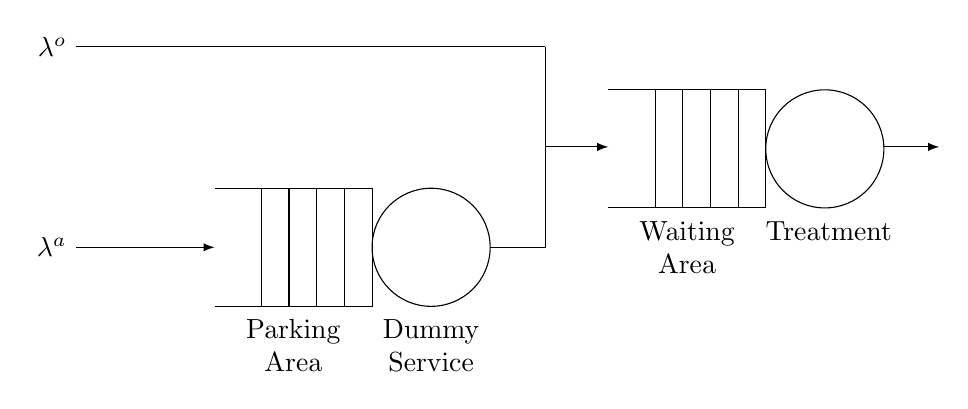
\begin{tikzpicture}[>=latex]
        % the rectangle with vertical rules (Queue 1)
        \draw (0,0) -- ++(2cm,0) -- ++(0,-1.5cm) -- ++(-2cm,0);
        \foreach \i in {1,...,4}
        \draw (2cm-\i*10pt,0) -- +(0,-1.5cm);
        
        % the circle (Queue 1)
        \draw (2.75,-0.75cm) circle [radius=0.75cm];

        % the rectangle with vertical rules (Queue 2)
        \draw (5,1.25) -- ++(2cm,0) -- ++(0,-1.5cm) -- ++(-2cm,0);
        \foreach \i in {1,...,4}
        \draw (7cm-\i*10pt,1.25) -- +(0,-1.5cm);

        % the circle (Queue 2)
        \draw (7.75,0.5) circle [radius=0.75cm];

        % the arrows and labels (Queue 1+2)
        \draw[-] (3.5,-0.75) -- +(20pt,0);
        \draw[<-] (0,-0.75) -- +(-50pt,0) node[left] {\( \lambda^a \)};
        \draw[->] (8.5,0.525) -- +(20pt,0);
        \node[align=center] at (1cm,-2cm) {Parking \\ Area};
        \node[align=center] at (2.75cm,-2cm) {Dummy \\ Service};
        \node[align=center] at (6cm,-0.75cm) {Waiting \\ Area};
        \node[align=center] at (7.8cm,-0.75cm) {Treatment \\ };
        
        \draw (4.2, 1.8) -- +(-169.5pt,0) node[left] {\( \lambda^o \)};
        \draw (4.2, 1.8) -- (4.2, -0.75);
        \draw[->] (4.2, 0.525) -- (5, 0.525);

    \end{tikzpicture}
\end{figure}


\begin{figure}
    \centering
    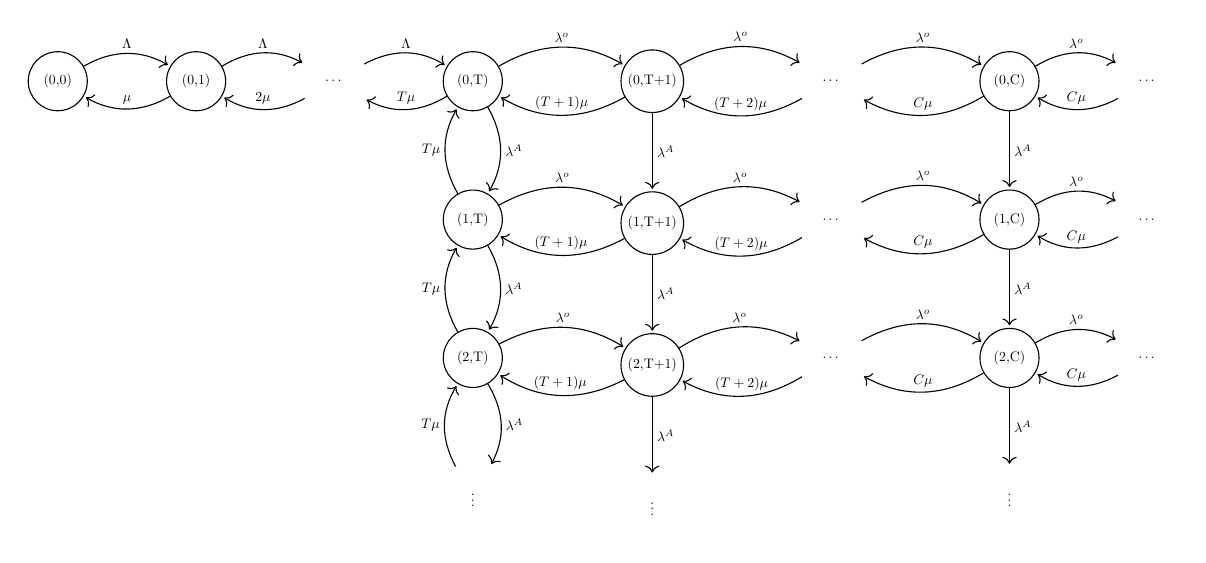
\begin{tikzpicture}[-, node distance = 1cm, auto, every node/.style={scale=0.5}]

        % Variables
        \tikzmath{
            let \altdist = 1.5cm;
            let \minsz = 1.5cm;
        }

        % First Line
        \node[state, minimum size=1.5cm] (zero) {(0,0)};
        \node[state, minimum size=1.5cm,  right=of zero] (one) {(0,1)};
        \node[draw=none, minimum size=1.5cm, right=of one] (two) {\dots};
        \node[state, minimum size=1.5cm, right=of two] (three) {(0,T)};
        \node[state, node distance = \altdist, minimum size=\minsz, right=of three] (four) {(0,T+1)};
        \node[draw=none, node distance = \altdist, minimum size=\minsz, right=of four] (five) {\dots};
        \node[state, node distance = \altdist, minimum size=\minsz, right=of five] (six) {(0,C)};
        \node[draw=none, minimum size=\minsz, right=of six] (seven) {\dots};

        % Second Line
        \node[state, minimum size=\minsz, below=of three] (three_one) {(1,T)};
        \node[state, minimum size=\minsz, below=of four] (four_one) {(1,T+1)};
        \node[draw=none, minimum size=\minsz, below=of five] (five_one) {\dots};
        \node[state, node distance = \altdist, minimum size=\minsz, right=of five_one] (six_one) {(1,C)};
        \node[draw=none, minimum size=\minsz, right=of six_one] (seven_one) {\dots};

        % Third Line
        \node[state, minimum size=\minsz, below=of three_one] (three_two) {(2,T)};
        \node[state, minimum size=\minsz, below=of four_one] (four_two) {(2,T+1)};
        \node[draw=none, minimum size=\minsz, below=of five_one] (five_two) {\dots};
        \node[state, node distance = \altdist, minimum size=\minsz, right=of five_two] (six_two) {(2,C)};
        \node[draw=none, minimum size=\minsz, right=of six_two] (seven_two) {\dots};

        % Fourth line
        \node[draw=none, minimum size=\minsz, below=of three_two] (three_three) {\vdots};
        \node[draw=none, minimum size=\minsz, below=of four_two] (four_three) {\vdots};
        \node[draw=none, minimum size=\minsz, below=of five_two] (five_three) {};
        \node[draw=none, node distance = \altdist, minimum size=\minsz, right=of five_three] (six_three) {\vdots};

        \draw[every loop]
            % First Horizontal Edges
            (zero) edge[bend left] node {\( \Lambda \)} (one)
            (one) edge[bend left] node [above] {\( \mu \)} (zero)
            (one) edge[bend left] node {\( \Lambda \)} (two)
            (two) edge[bend left] node [above] {\( 2 \mu \)} (one)
            (two) edge[bend left] node {\( \Lambda \)} (three)
            (three) edge[bend left] node [above] {\( T \mu \)} (two)
            (three) edge[bend left] node {\( \lambda^o \)} (four)
            (four) edge[bend left] node [above] {\( (T+1) \mu \)} (three)
            (four) edge[bend left] node {\( \lambda^o \)} (five)
            (five) edge[bend left] node [above] {\( (T+2) \mu \)} (four)
            (five) edge[bend left] node {\( \lambda^o \)} (six)
            (six) edge[bend left] node [above] {\( C\mu \)} (five)
            (six) edge[bend left] node {\( \lambda^o \)} (seven)
            (seven) edge[bend left] node [above] {\( C\mu \)} (six)

            % Second Horizontal Edges
            (three_one) edge[bend left] node {\( \lambda^o \)} (four_one)
            (four_one) edge[bend left] node [above] {\( (T+1) \mu \)} (three_one)
            (four_one) edge[bend left] node {\( \lambda^o \)} (five_one)
            (five_one) edge[bend left] node [above] {\( (T+2) \mu \)} (four_one)
            (five_one) edge[bend left] node {\( \lambda^o \)} (six_one)
            (six_one) edge[bend left] node [above] {\( C\mu \)} (five_one)
            (six_one) edge[bend left] node {\( \lambda^o \)} (seven_one)
            (seven_one) edge[bend left] node [above] {\( C\mu \)} (six_one)

            % Third Horizontal Edges
            (three_two) edge[bend left] node {\( \lambda^o \)} (four_two)
            (four_two) edge[bend left] node [above] {\( (T+1) \mu \)} (three_two)
            (four_two) edge[bend left] node {\( \lambda^o \)} (five_two)
            (five_two) edge[bend left] node [above] {\( (T+2) \mu \)} (four_two)
            (five_two) edge[bend left] node {\( \lambda^o \)} (six_two)
            (six_two) edge[bend left] node [above] {\( C\mu \)} (five_two)
            (six_two) edge[bend left] node {\( \lambda^o \)} (seven_two)
            (seven_two) edge[bend left] node [above] {\( C\mu \)} (six_two)

            % First Vertical Edges
            (three) edge[bend left] node {\( \lambda^A \)} (three_one)
            (three_one) edge[bend left] node {\( T \mu \)} (three)
            (three_one) edge[bend left] node {\( \lambda^A \)} (three_two)
            (three_two) edge[bend left] node {\( T\mu \)} (three_one)
            (three_two) edge[bend left] node {\( \lambda^A \)} (three_three)
            (three_three) edge[bend left] node {\( T\mu \)} (three_two)

            % Second Vertical Edges
            (four) edge node {\( \lambda^A \)} (four_one)
            (four_one) edge node {\( \lambda^A \)} (four_two)
            (four_two) edge node {\( \lambda^A \)} (four_three)

            %Third Vertical Edges
            (six) edge node {\( \lambda^A \)} (six_one)
            (six_one) edge node {\( \lambda^A \)} (six_two)
            (six_two) edge node {\( \lambda^A \)} (six_three)
            ;       
    \end{tikzpicture}
    \caption{Markov chains} 
    \label{Markov_2}
\end{figure}



\begin{figure}
    \centering
    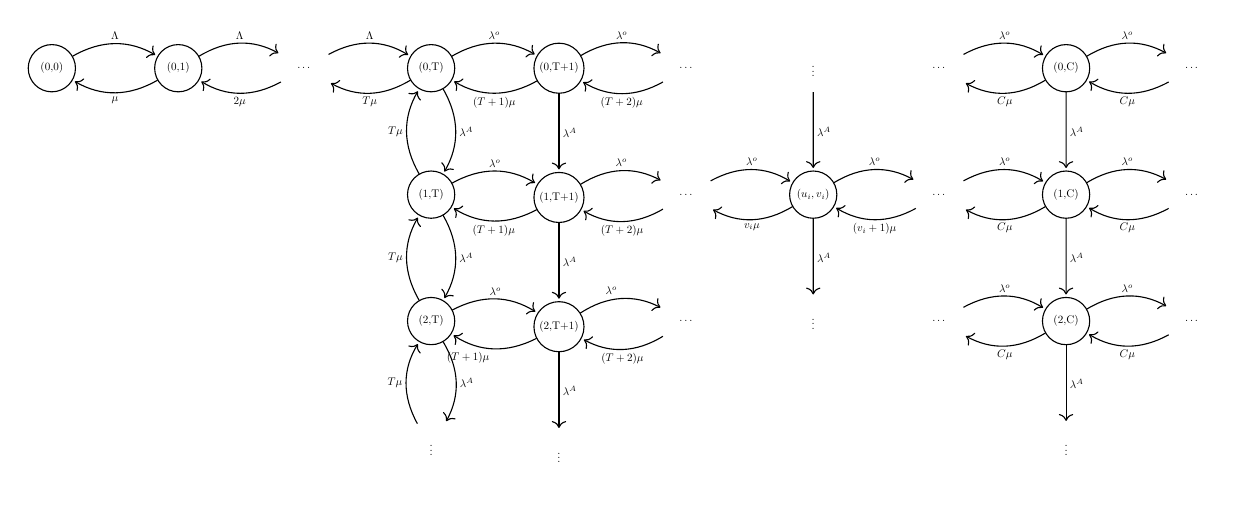
\begin{tikzpicture}[-, node distance = 1cm, auto, every node/.style={scale=0.4}]

        % Variables
        \tikzmath{
            let \altdist = 1cm;
            let \minsz = 1.5cm;
        }

        % First Line
        \node[state, minimum size=1.5cm] (zero) {(0,0)};
        \node[state, minimum size=1.5cm,  right=of zero] (one) {(0,1)};
        \node[draw=none, minimum size=1.5cm, right=of one] (two) {\dots};
        \node[state, minimum size=1.5cm, right=of two] (three) {(0,T)};
        \node[state, node distance = \altdist, minimum size=\minsz, right=of three] (four) {(0,T+1)};
        \node[draw=none, minimum size=\minsz, right=of four] (five) {\dots};
        \node[draw=none, minimum size=\minsz, right=of five] (six) {\vdots};
        \node[draw=none, minimum size=\minsz, right=of six] (seven) {\dots};
        \node[state, minimum size=\minsz, right=of seven] (eight) {(0,C)};
        \node[draw=none, minimum size=\minsz, right=of eight] (nine) {\dots};


        % Second Line
        \node[state, minimum size=\minsz, below=of three] (three_one) {(1,T)};
        \node[state, minimum size=\minsz, below=of four] (four_one) {(1,T+1)};
        \node[draw=none, minimum size=\minsz, below=of five] (five_one) {\dots};
        \node[state, node distance = \altdist, minimum size=\minsz, right=of five_one] (six_one) {\( (u_i, v_i) \)};
        \node[draw=none, minimum size=\minsz, right=of six_one] (seven_one) {\dots};
        \node[state, node distance = \altdist, minimum size=\minsz, right=of seven_one] (eight_one) {(1,C)};
        \node[draw=none, minimum size=\minsz, right=of eight_one] (nine_one) {\dots};
        

        % Third Line
        \node[state, minimum size=\minsz, below=of three_one] (three_two) {(2,T)};
        \node[state, minimum size=\minsz, below=of four_one] (four_two) {(2,T+1)};
        \node[draw=none, minimum size=\minsz, below=of five_one] (five_two) {\dots};
        \node[draw=none, node distance = \altdist, minimum size=\minsz, right=of five_two] (six_two) {\vdots};
        \node[draw=none, minimum size=\minsz, right=of six_two] (seven_two) {\dots};
        \node[state, node distance = \altdist, minimum size=\minsz, right=of seven_two] (eight_two) {(2,C)};
        \node[draw=none, minimum size=\minsz, right=of eight_two] (nine_two) {\dots};

        % Fourth line
        \node[draw=none, minimum size=\minsz, below=of three_two] (three_three) {\vdots};
        \node[draw=none, minimum size=\minsz, below=of four_two] (four_three) {\vdots};
        \node[draw=none, minimum size=\minsz, below=of five_two] (five_three) {};
        \node[draw=none, node distance = \altdist, minimum size=\minsz, right=of five_three] (six_three) {};
        \node[draw=none, node distance = \altdist, minimum size=\minsz, below=of eight_two] (eight_three) {\vdots};


        \draw[every loop]
            % First Horizontal Edges
            (zero) edge[bend left] node {\( \Lambda \)} (one)
            (one) edge[bend left] node {\( \mu \)} (zero)
            (one) edge[bend left] node {\( \Lambda \)} (two)
            (two) edge[bend left] node {\( 2 \mu \)} (one)
            (two) edge[bend left] node {\( \Lambda \)} (three)
            (three) edge[bend left] node {\( T \mu \)} (two)
            (three) edge[bend left] node {\( \lambda^o \)} (four)
            (four) edge[bend left] node {\( (T+1) \mu \)} (three)
            (four) edge[bend left] node {\( \lambda^o \)} (five)
            (five) edge[bend left] node {\( (T+2) \mu \)} (four)
            % (five) edge[bend left] node {\( \lambda^o \)} (six)
            % (six) edge[bend left] node [above] {\( C\mu \)} (five)
            % (six) edge[bend left] node {\( \lambda^o \)} (seven)
            % (seven) edge[bend left] node [above] {\( C\mu \)} (six)
            (seven) edge[bend left] node {\( \lambda^o \)} (eight)
            (eight) edge[bend left] node {\( C\mu \)} (seven)
            (eight) edge[bend left] node {\( \lambda^o \)} (nine)
            (nine) edge[bend left] node {\( C\mu \)} (eight)

            % Second Horizontal Edges
            (three_one) edge[bend left] node {\(\lambda^o\)} (four_one)
            (four_one) edge[bend left] node {\( (T+1) \mu \)} (three_one)
            (four_one) edge[bend left] node {\( \lambda^o \)} (five_one)
            (five_one) edge[bend left] node {\( (T+2) \mu \)} (four_one)
            (five_one) edge[bend left] node {\( \lambda^o \)} (six_one)
            (six_one) edge[bend left] node {\( v_i\mu \)} (five_one)
            (six_one) edge[bend left] node {\( \lambda^o \)} (seven_one)
            (seven_one) edge[bend left] node {\( (v_i+1)\mu \)} (six_one)
            (seven_one) edge[bend left] node {\( \lambda^o \)} (eight_one)
            (eight_one) edge[bend left] node {\( C\mu \)} (seven_one)
            (eight_one) edge[bend left] node {\( \lambda^o \)} (nine_one)
            (nine_one) edge[bend left] node {\( C\mu \)} (eight_one)

            % Third Horizontal Edges
            (three_two) edge[bend left] node {\( \lambda^o \)} (four_two)
            (four_two) edge[bend left] node {\( (T+1) \mu \)} (three_two)
            (four_two) edge[bend left] node {\( \lambda^o \)} (five_two)
            (five_two) edge[bend left] node {\( (T+2) \mu \)} (four_two)
            % (five_two) edge[bend left] node {\( \lambda^o \)} (six_two)
            % (six_two) edge[bend left] node [above] {\( C\mu \)} (five_two)
            % (six_two) edge[bend left] node {\( \lambda^o \)} (seven_two)
            % (seven_two) edge[bend left] node [above] {\( C\mu \)} (six_two)
            (seven_two) edge[bend left] node {\( \lambda^o \)} (eight_two)
            (eight_two) edge[bend left] node {\( C\mu \)} (seven_two)
            (eight_two) edge[bend left] node {\( \lambda^o \)} (nine_two)
            (nine_two) edge[bend left] node {\( C\mu \)} (eight_two)

            % First Vertical Edges
            (three) edge[bend left] node {\( \lambda^A \)} (three_one)
            (three_one) edge[bend left] node {\( T \mu \)} (three)
            (three_one) edge[bend left] node {\( \lambda^A \)} (three_two)
            (three_two) edge[bend left] node {\( T\mu \)} (three_one)
            (three_two) edge[bend left] node {\( \lambda^A \)} (three_three)
            (three_three) edge[bend left] node {\( T\mu \)} (three_two)

            % Second Vertical Edges
            (four) edge node {\( \lambda^A \)} (four_one)
            (four_one) edge node {\( \lambda^A \)} (four_two)
            (four_two) edge node {\( \lambda^A \)} (four_three)

            % Third Vertical Edges
            (six) edge node {\( \lambda^A \)} (six_one)
            (six_one) edge node {\( \lambda^A \)} (six_two)
            % (six_two) edge node {\( \lambda^A \)} (six_three)

            % Fourth Vertical Edges
            (eight) edge node {\( \lambda^A \)} (eight_one)
            (eight_one) edge node {\( \lambda^A \)} (eight_two)
            (eight_two) edge node {\( \lambda^A \)} (eight_three)
            ;       
    \end{tikzpicture}
    \caption{Markov chains} 
    \label{Markov_3}
\end{figure}


\begin{figure}
    \centering
    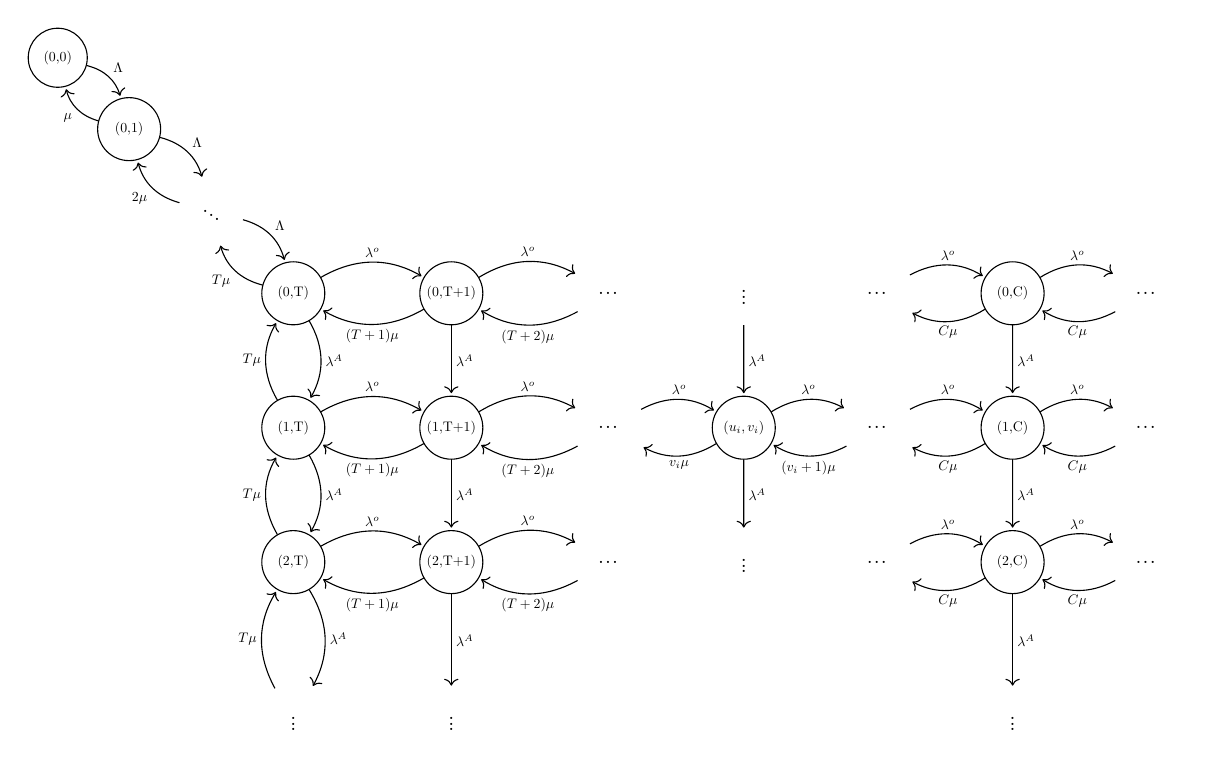
\begin{tikzpicture}[-, node distance = 0.9cm, auto, every node/.style={scale=0.5}]

        % Variables
        \tikzmath{
            let \initdist = 0.5cm;
            let \altdist = 1.2cm;
            let \minsz = 1.6cm;
            let \leftOne = -0.8;
            let \rightOne = 2.2;
            let \upOne = 0.8;
            let \downOne = -2.2;
            let \leftTwo = 2.25;
            let \rightTwo = 14.2;
            let \upTwo = -2.35;
            let \downTwo = -8.8;
        }

        % % Rectangle for S1
        % \draw[ultra thin, dashed] (\leftOne, \downOne) -- (\leftOne, \upOne);
        % \draw[ultra thin, dashed] (\leftOne, \upOne) -- (\rightOne, \upOne);
        % \draw[ultra thin, dashed] (\rightOne, \upOne) -- node {\Huge{\( \quad S_1 \)}}(\rightOne, \downOne);
        % \draw[ultra thin, dashed] (\rightOne, \downOne) -- (\leftOne, \downOne);

        % % Rectangle for S2
        % \draw[ultra thin, dashed] (\leftTwo, \downTwo) -- node {\Huge{\( S_2 \quad \)}}(\leftTwo, \upTwo);
        % \draw[ultra thin, dashed] (\leftTwo, \upTwo) -- (\rightTwo, \upTwo);
        % \draw[ultra thin, dashed] (\rightTwo, \upTwo) -- (\rightTwo, \downTwo);
        % \draw[ultra thin, dashed] (\rightTwo, \downTwo) -- (\leftTwo, \downTwo);

        % First Line
        \node[state, minimum size=1.5cm] (zero) {(0,0)};
        \node[state, node distance = \initdist, minimum size=\minsz, below right=of zero] (one) {(0,1)};
        \node[draw=none, node distance = \initdist, minimum size=\minsz, below right=of one] (two) {\textbf{\( \ddots \)}};
        \node[state, node distance = \initdist, minimum size=\minsz, below right=of two] (three) {(0,T)};
        \node[state, node distance = \altdist, minimum size=\minsz, right=of three] (four) {(0,T+1)};
        \node[draw=none, node distance = \altdist, minimum size=\minsz, right=of four] (five) {\textbf{\dots}};
        \node[draw=none, minimum size=\minsz, right=of five] (six) {\textbf{\vdots}};
        \node[draw=none, minimum size=\minsz, right=of six] (seven) {\textbf{\dots}};
        \node[state, minimum size=\minsz, right=of seven] (eight) {(0,C)};
        \node[draw=none, minimum size=\minsz, right=of eight] (nine) {\textbf{\dots}};


        % Second Line
        \node[state, minimum size=\minsz, below=of three] (three_one) {(1,T)};
        \node[state, minimum size=\minsz, below=of four] (four_one) {(1,T+1)};
        \node[draw=none, minimum size=\minsz, below=of five] (five_one) {\textbf{\dots}};
        \node[state, minimum size=\minsz, right=of five_one] (six_one) {\( (u_i, v_i) \)};
        \node[draw=none, minimum size=\minsz, right=of six_one] (seven_one) {\textbf{\dots}};
        \node[state, minimum size=\minsz, right=of seven_one] (eight_one) {(1,C)};
        \node[draw=none, minimum size=\minsz, right=of eight_one] (nine_one) {\textbf{\dots}};
        

        % Third Line
        \node[state, minimum size=\minsz, below=of three_one] (three_two) {(2,T)};
        \node[state, minimum size=\minsz, below=of four_one] (four_two) {(2,T+1)};
        \node[draw=none, minimum size=\minsz, below=of five_one] (five_two) {\textbf{\dots}};
        \node[draw=none, minimum size=\minsz, right=of five_two] (six_two) {\textbf{\vdots}};
        \node[draw=none, minimum size=\minsz, right=of six_two] (seven_two) {\textbf{\dots}};
        \node[state, minimum size=\minsz, right=of seven_two] (eight_two) {(2,C)};
        \node[draw=none, minimum size=\minsz, right=of eight_two] (nine_two) {\textbf{\dots}};

        % Fourth line
        \node[draw=none, node distance = \altdist, minimum size=\minsz, below=of three_two] (three_three) {\textbf{\vdots}};
        \node[draw=none, node distance = \altdist, minimum size=\minsz, below=of four_two] (four_three) {\textbf{\vdots}};
        \node[draw=none, node distance = \altdist, minimum size=\minsz, below=of five_two] (five_three) {};
        \node[draw=none, node distance = \altdist, minimum size=\minsz, below=of six_two] (six_three) {};
        \node[draw=none, node distance = \altdist, minimum size=\minsz, below=of eight_two] (eight_three) {\textbf{\vdots}};


        \draw[every loop]
            % First Horizontal Edges
            (zero) edge[bend left] node {\( \Lambda \)} (one)
            (one) edge[bend left] node {\( \mu \)} (zero)
            (one) edge[bend left] node {\( \Lambda \)} (two)
            (two) edge[bend left] node {\( 2 \mu \)} (one)
            (two) edge[bend left] node {\( \Lambda \)} (three)
            (three) edge[bend left] node {\( T \mu \)} (two)
            (three) edge[bend left] node {\( \lambda^o \)} (four)
            (four) edge[bend left] node {\( (T+1) \mu \)} (three)
            (four) edge[bend left] node {\( \lambda^o \)} (five)
            (five) edge[bend left] node {\( (T+2) \mu \)} (four)
            % (five) edge[bend left] node {\( \lambda^o \)} (six)
            % (six) edge[bend left] node [above] {\( C\mu \)} (five)
            % (six) edge[bend left] node {\( \lambda^o \)} (seven)
            % (seven) edge[bend left] node [above] {\( C\mu \)} (six)
            (seven) edge[bend left] node {\( \lambda^o \)} (eight)
            (eight) edge[bend left] node {\( C\mu \)} (seven)
            (eight) edge[bend left] node {\( \lambda^o \)} (nine)
            (nine) edge[bend left] node {\( C\mu \)} (eight)

            % Second Horizontal Edges
            (three_one) edge[bend left] node {\( \lambda^o \)} (four_one)
            (four_one) edge[bend left] node {\( (T+1) \mu \)} (three_one)
            (four_one) edge[bend left] node {\( \lambda^o \)} (five_one)
            (five_one) edge[bend left] node {\( (T+2) \mu \)} (four_one)
            (five_one) edge[bend left] node {\( \lambda^o \)} (six_one)
            (six_one) edge[bend left] node {\( v_i\mu \)} (five_one)
            (six_one) edge[bend left] node {\( \lambda^o \)} (seven_one)
            (seven_one) edge[bend left] node {\( (v_i+1)\mu \)} (six_one)
            (seven_one) edge[bend left] node {\( \lambda^o \)} (eight_one)
            (eight_one) edge[bend left] node {\( C\mu \)} (seven_one)
            (eight_one) edge[bend left] node {\( \lambda^o \)} (nine_one)
            (nine_one) edge[bend left] node {\( C\mu \)} (eight_one)

            % Third Horizontal Edges
            (three_two) edge[bend left] node {\( \lambda^o \)} (four_two)
            (four_two) edge[bend left] node [below] {\( (T+1) \mu \)} (three_two)
            (four_two) edge[bend left] node {\( \lambda^o \)} (five_two)
            (five_two) edge[bend left] node {\( (T+2) \mu \)} (four_two)
            % (five_two) edge[bend left] node {\( \lambda^o \)} (six_two)
            % (six_two) edge[bend left] node [above] {\( C\mu \)} (five_two)
            % (six_two) edge[bend left] node {\( \lambda^o \)} (seven_two)
            % (seven_two) edge[bend left] node [above] {\( C\mu \)} (six_two)
            (seven_two) edge[bend left] node {\( \lambda^o \)} (eight_two)
            (eight_two) edge[bend left] node {\( C\mu \)} (seven_two)
            (eight_two) edge[bend left] node {\( \lambda^o \)} (nine_two)
            (nine_two) edge[bend left] node {\( C\mu \)} (eight_two)

            % First Vertical Edges
            (three) edge[bend left] node {\( \lambda^A \)} (three_one)
            (three_one) edge[bend left] node {\( T \mu \)} (three)
            (three_one) edge[bend left] node {\( \lambda^A \)} (three_two)
            (three_two) edge[bend left] node {\( T\mu \)} (three_one)
            (three_two) edge[bend left] node {\( \lambda^A \)} (three_three)
            (three_three) edge[bend left] node {\( T\mu \)} (three_two)

            % Second Vertical Edges
            (four) edge node {\( \lambda^A \)} (four_one)
            (four_one) edge node {\( \lambda^A \)} (four_two)
            (four_two) edge node {\( \lambda^A \)} (four_three)

            % Third Vertical Edges
            (six) edge node {\( \lambda^A \)} (six_one)
            (six_one) edge node {\( \lambda^A \)} (six_two)
            % (six_two) edge node {\( \lambda^A \)} (six_three)

            % Fourth Vertical Edges
            (eight) edge node {\( \lambda^A \)} (eight_one)
            (eight_one) edge node {\( \lambda^A \)} (eight_two)
            (eight_two) edge node {\( \lambda^A \)} (eight_three)
            ;       
    \end{tikzpicture}
    \caption{Markov chains} 
    \label{Markov_4}
\end{figure}




\begin{figure}
    \centering
    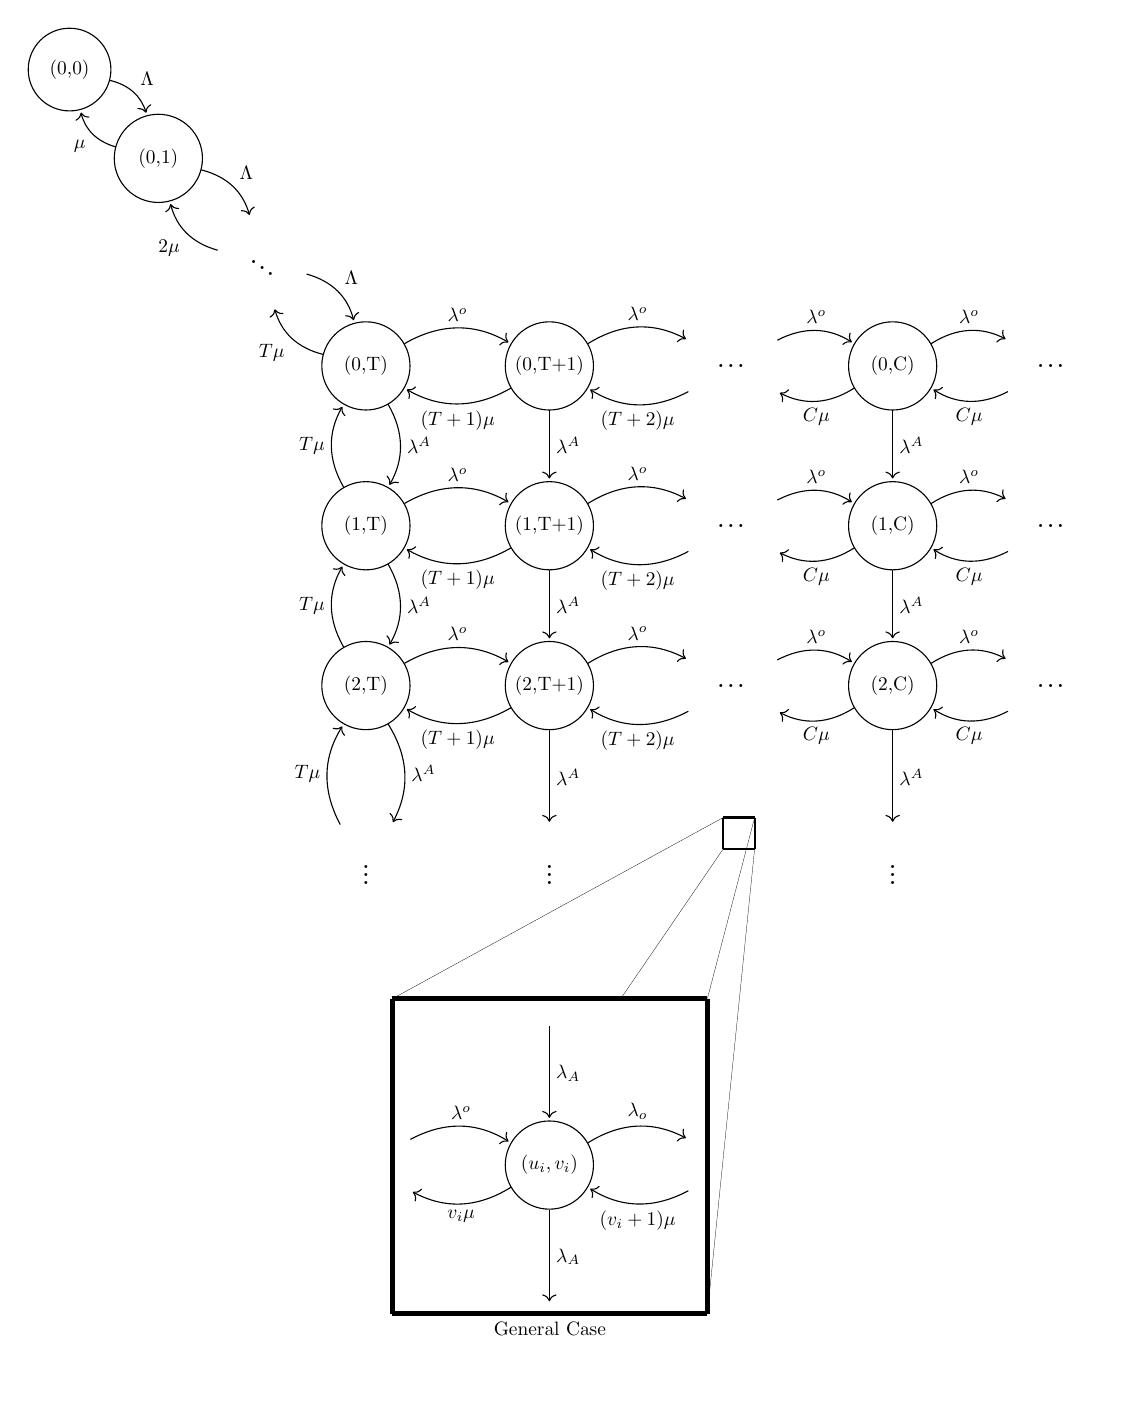
\begin{tikzpicture}[-, node distance = 0.9cm, auto, every node/.style={scale=0.7}]

        % Markov chain variables
        \tikzmath{
            let \initdist = 0.5cm;
            let \altdist = 1.2cm;
            let \minsz = 1.6cm;
        }

        % S_1 and S_2 rectangles
        \tikzmath{
            let \leftOne = -0.8;
            let \rightOne = 2.7;
            let \upOne = 0.8;
            let \downOne = -2.7;
            let \leftTwo = 2.8;
            let \rightTwo = 13;
            let \upTwo = -2.95;
            let \downTwo = -16.4;
        }

        % General case variables
        \tikzmath{
            let \GCsmallx = 8.3;
            let \GCsmally = -9.5;
            let \GCbigx = 4.1;
            let \GCbigy = -11.8;
        }

        % % Rectangle for S1
        % \draw[ultra thin, dashed] (\leftOne, \downOne) -- (\leftOne, \upOne);
        % \draw[ultra thin, dashed] (\leftOne, \upOne) -- (\rightOne, \upOne);
        % \draw[ultra thin, dashed] (\rightOne, \upOne) -- node {\Huge{\( \quad S_1 \)}}(\rightOne, \downOne);
        % \draw[ultra thin, dashed] (\rightOne, \downOne) -- (\leftOne, \downOne);

        % % Rectangle for S2
        % \draw[ultra thin, dashed] (\leftTwo, \downTwo) -- node {\Huge{\( S_2 \quad \)}}(\leftTwo, \upTwo);
        % \draw[ultra thin, dashed] (\leftTwo, \upTwo) -- (\rightTwo, \upTwo);
        % \draw[ultra thin, dashed] (\rightTwo, \upTwo) -- (\rightTwo, \downTwo);
        % \draw[ultra thin, dashed] (\rightTwo, \downTwo) -- (\leftTwo, \downTwo);

        % Small square of general case
        \draw [thick] (\GCsmallx, \GCsmally) -- node {} (\GCsmallx + 0.4, \GCsmally);
        \draw [thick] (\GCsmallx + 0.4, \GCsmally) -- node {} (\GCsmallx + 0.4, \GCsmally - 0.4);
        \draw [thick] (\GCsmallx + 0.4, \GCsmally - 0.4) -- node {} (\GCsmallx, \GCsmally - 0.4);
        \draw [thick] (\GCsmallx, \GCsmally - 0.4) -- node {} (\GCsmallx, \GCsmally);


        % Dashed lines to from small square to big one 
        \draw [ultra thin] (\GCsmallx, \GCsmally) -- node {} (\GCbigx, \GCbigy);
        \draw [ultra thin] (\GCsmallx + 0.4, \GCsmally) -- node {} (\GCbigx + 4, \GCbigy);
        \draw [ultra thin] (\GCsmallx, \GCsmally - 0.4) -- node {} (7, \GCbigy);
        \draw [ultra thin] (\GCsmallx + 0.4, \GCsmally - 0.4) -- node {} (\GCbigx + 4, \GCbigy - 4);
        
        % Big Square of general case
        \draw [ultra thick] (\GCbigx, \GCbigy) -- node {} (\GCbigx + 4, \GCbigy);
        \draw [ultra thick] (\GCbigx + 4, \GCbigy) -- node {} (\GCbigx + 4, \GCbigy - 4);
        \draw [ultra thick] (\GCbigx + 4, \GCbigy - 4) -- node {General Case} (\GCbigx, \GCbigy - 4);
        \draw [ultra thick] (\GCbigx, \GCbigy - 4) -- node {} (\GCbigx, \GCbigy);

        % First Line
        \node[state, minimum size=1.5cm] (zero) {(0,0)};
        \node[state, node distance = \initdist, minimum size=\minsz, below right=of zero] (one) {(0,1)};
        \node[draw=none, node distance = \initdist, minimum size=\minsz, below right=of one] (two) {\textbf{\( \ddots \)}};
        \node[state, node distance = \initdist, minimum size=\minsz, below right=of two] (three) {(0,T)};
        \node[state, node distance = \altdist, minimum size=\minsz, right=of three] (four) {(0,T+1)};
        \node[draw=none, node distance = \altdist, minimum size=\minsz, right=of four] (five) {\textbf{\dots}};
        \node[state, minimum size=\minsz, right=of five] (six) {(0,C)};
        \node[draw=none, minimum size=\minsz, right=of six] (seven) {\textbf{\dots}};

        % Second Line
        \node[state, minimum size=\minsz, below=of three] (three_one) {(1,T)};
        \node[state, minimum size=\minsz, below=of four] (four_one) {(1,T+1)};
        \node[draw=none, minimum size=\minsz, below=of five] (five_one) {\textbf{\dots}};
        \node[state, minimum size=\minsz, right=of five_one] (six_one) {(1,C)};
        \node[draw=none, minimum size=\minsz, right=of six_one] (seven_one) {\textbf{\dots}};
        
        % Third Line
        \node[state, minimum size=\minsz, below=of three_one] (three_two) {(2,T)};
        \node[state, minimum size=\minsz, below=of four_one] (four_two) {(2,T+1)};
        \node[draw=none, minimum size=\minsz, below=of five_one] (five_two) {\textbf{\dots}};
        \node[state, minimum size=\minsz, right=of five_two] (six_two) {(2,C)};
        \node[draw=none, minimum size=\minsz, right=of six_two] (seven_two) {\textbf{\dots}};

        % Fourth line
        \node[draw=none, node distance = \altdist, minimum size=\minsz, below=of three_two] (three_three) {\textbf{\vdots}};
        \node[draw=none, node distance = \altdist, minimum size=\minsz, below=of four_two] (four_three) {\textbf{\vdots}};
        \node[draw=none, node distance = 2cm, minimum size=\minsz, below=of five_two] (five_three) {};
        \node[draw=none, node distance = \altdist, minimum size=\minsz, below=of six_two] (six_three) {\textbf{\vdots}};

        % Fifth line
        % \node[state, node distance = \altdist, minimum size=\minsz, below=of five_three] (general_case_mid) {\( (u_i, v_i) \)};
        \node[draw=none, node distance = 0.3cm, minimum size=\minsz, below=of four_three] (general_case_up) {};
        \node[state, node distance = \altdist, minimum size=\minsz, below=of general_case_up] (general_case_mid) {\( (u_i, v_i) \)};

        \node[draw=none, node distance = \altdist, minimum size=\minsz, below=of general_case_mid] (general_case_down) {};
        \node[draw=none, node distance = \altdist, minimum size=\minsz, left=of general_case_mid] (general_case_left) {};
        \node[draw=none, node distance = \altdist, minimum size=\minsz, right=of general_case_mid] (general_case_right) {};

        \draw[every loop]
            % First Horizontal Edges
            (zero) edge[bend left] node {\( \Lambda \)} (one)
            (one) edge[bend left] node {\( \mu \)} (zero)
            (one) edge[bend left] node {\( \Lambda \)} (two)
            (two) edge[bend left] node {\( 2 \mu \)} (one)
            (two) edge[bend left] node {\( \Lambda \)} (three)
            (three) edge[bend left] node {\( T \mu \)} (two)
            (three) edge[bend left] node {\( \lambda^o \)} (four)
            (four) edge[bend left] node {\( (T+1) \mu \)} (three)
            (four) edge[bend left] node {\( \lambda^o \)} (five)
            (five) edge[bend left] node {\( (T+2) \mu \)} (four)
            (five) edge[bend left] node {\( \lambda^o \)} (six)
            (six) edge[bend left] node {\( C\mu \)} (five)
            (six) edge[bend left] node {\( \lambda^o \)} (seven)
            (seven) edge[bend left] node {\( C\mu \)} (six)

            % Second Horizontal Edges
            (three_one) edge[bend left] node {\( \lambda^o \)} (four_one)
            (four_one) edge[bend left] node {\( (T+1) \mu \)} (three_one)
            (four_one) edge[bend left] node {\( \lambda^o \)} (five_one)
            (five_one) edge[bend left] node {\( (T+2) \mu \)} (four_one)
            (five_one) edge[bend left] node {\( \lambda^o \)} (six_one)
            (six_one) edge[bend left] node {\( C\mu \)} (five_one)
            (six_one) edge[bend left] node {\( \lambda^o \)} (seven_one)
            (seven_one) edge[bend left] node {\( C\mu \)} (six_one)

            % Third Horizontal Edges
            (three_two) edge[bend left] node {\( \lambda^o \)} (four_two)
            (four_two) edge[bend left] node [below] {\( (T+1) \mu \)} (three_two)
            (four_two) edge[bend left] node {\( \lambda^o \)} (five_two)
            (five_two) edge[bend left] node {\( (T+2) \mu \)} (four_two)
            (five_two) edge[bend left] node {\( \lambda^o \)} (six_two)
            (six_two) edge[bend left] node {\( C\mu \)} (five_two)
            (six_two) edge[bend left] node {\( \lambda^o \)} (seven_two)
            (seven_two) edge[bend left] node {\( C\mu \)} (six_two)

            % First Vertical Edges
            (three) edge[bend left] node {\( \lambda^A \)} (three_one)
            (three_one) edge[bend left] node {\( T \mu \)} (three)
            (three_one) edge[bend left] node {\( \lambda^A \)} (three_two)
            (three_two) edge[bend left] node {\( T\mu \)} (three_one)
            (three_two) edge[bend left] node {\( \lambda^A \)} (three_three)
            (three_three) edge[bend left] node {\( T\mu \)} (three_two)

            % Second Vertical Edges
            (four) edge node {\( \lambda^A \)} (four_one)
            (four_one) edge node {\( \lambda^A \)} (four_two)
            (four_two) edge node {\( \lambda^A \)} (four_three)

            % Fourth Vertical Edges
            (six) edge node {\( \lambda^A \)} (six_one)
            (six_one) edge node {\( \lambda^A \)} (six_two)
            (six_two) edge node {\( \lambda^A \)} (six_three)

            % General Case
            (general_case_left) edge[bend left] node {\( \lambda^o \)} (general_case_mid)
            (general_case_mid) edge[bend left] node {\( v_i \mu \)} (general_case_left)
            (general_case_right) edge[bend left] node {\( (v_i +1) \mu \)} (general_case_mid)
            (general_case_mid) edge[bend left] node {\( \lambda_o \)} (general_case_right)
            % (five_three) edge node {\( \lambda_A \)} (general_case_mid)
            (general_case_up) edge node {\( \lambda_A \)} (general_case_mid)
            (general_case_mid) edge node {\( \lambda_A \)} (general_case_down)
            ;
    \end{tikzpicture}
    \caption{Markov chain} 
    \label{Markov_5}
\end{figure}



% Markov Chains
\section{Figures that might be useful}
\begin{figure}[h]
    \centering
    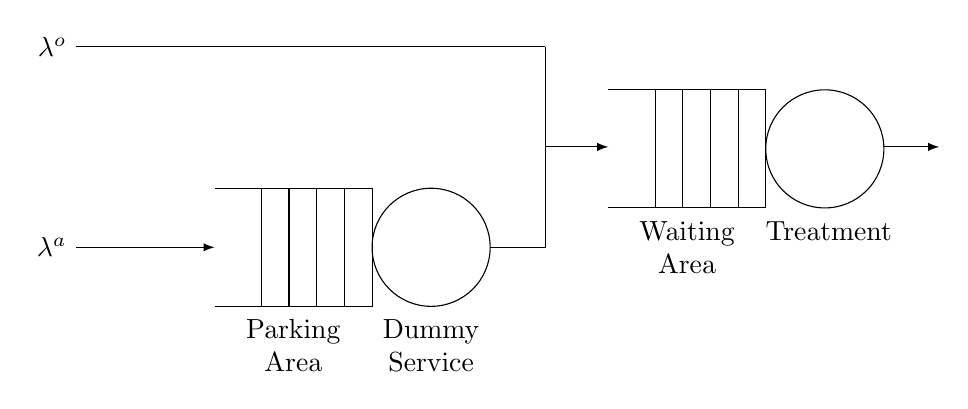
\begin{tikzpicture}[>=latex]
        % the rectangle with vertical rules (Queue 1)
        \draw (0,0) -- ++(2cm,0) -- ++(0,-1.5cm) -- ++(-2cm,0);
        \foreach \i in {1,...,4}
        \draw (2cm-\i*10pt,0) -- +(0,-1.5cm);
        
        % the circle (Queue 1)
        \draw (2.75,-0.75cm) circle [radius=0.75cm];

        % the rectangle with vertical rules (Queue 2)
        \draw (5,1.25) -- ++(2cm,0) -- ++(0,-1.5cm) -- ++(-2cm,0);
        \foreach \i in {1,...,4}
        \draw (7cm-\i*10pt,1.25) -- +(0,-1.5cm);

        % the circle (Queue 2)
        \draw (7.75,0.5) circle [radius=0.75cm];

        % the arrows and labels (Queue 1+2)
        \draw[-] (3.5,-0.75) -- +(20pt,0);
        \draw[<-] (0,-0.75) -- +(-50pt,0) node[left] {\( \lambda^a \)};
        \draw[->] (8.5,0.525) -- +(20pt,0);
        \node[align=center] at (1cm,-2cm) {Parking \\ Area};
        \node[align=center] at (2.75cm,-2cm) {Dummy \\ Service};
        \node[align=center] at (6cm,-0.75cm) {Waiting \\ Area};
        \node[align=center] at (7.8cm,-0.75cm) {Treatment \\ };
        
        \draw (4.2, 1.8) -- +(-169.5pt,0) node[left] {\( \lambda^o \)};
        \draw (4.2, 1.8) -- (4.2, -0.75);
        \draw[->] (4.2, 0.525) -- (5, 0.525);

    \end{tikzpicture}
\end{figure}


\begin{figure}
    \centering
    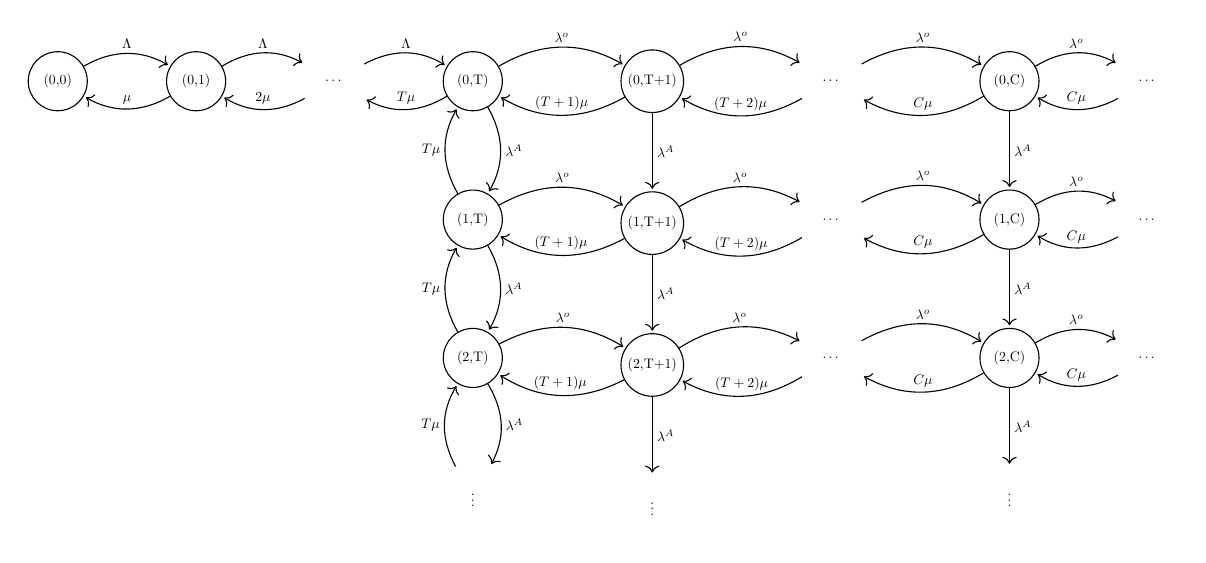
\begin{tikzpicture}[-, node distance = 1cm, auto, every node/.style={scale=0.5}]

        % Variables
        \tikzmath{
            let \altdist = 1.5cm;
            let \minsz = 1.5cm;
        }

        % First Line
        \node[state, minimum size=1.5cm] (zero) {(0,0)};
        \node[state, minimum size=1.5cm,  right=of zero] (one) {(0,1)};
        \node[draw=none, minimum size=1.5cm, right=of one] (two) {\dots};
        \node[state, minimum size=1.5cm, right=of two] (three) {(0,T)};
        \node[state, node distance = \altdist, minimum size=\minsz, right=of three] (four) {(0,T+1)};
        \node[draw=none, node distance = \altdist, minimum size=\minsz, right=of four] (five) {\dots};
        \node[state, node distance = \altdist, minimum size=\minsz, right=of five] (six) {(0,C)};
        \node[draw=none, minimum size=\minsz, right=of six] (seven) {\dots};

        % Second Line
        \node[state, minimum size=\minsz, below=of three] (three_one) {(1,T)};
        \node[state, minimum size=\minsz, below=of four] (four_one) {(1,T+1)};
        \node[draw=none, minimum size=\minsz, below=of five] (five_one) {\dots};
        \node[state, node distance = \altdist, minimum size=\minsz, right=of five_one] (six_one) {(1,C)};
        \node[draw=none, minimum size=\minsz, right=of six_one] (seven_one) {\dots};

        % Third Line
        \node[state, minimum size=\minsz, below=of three_one] (three_two) {(2,T)};
        \node[state, minimum size=\minsz, below=of four_one] (four_two) {(2,T+1)};
        \node[draw=none, minimum size=\minsz, below=of five_one] (five_two) {\dots};
        \node[state, node distance = \altdist, minimum size=\minsz, right=of five_two] (six_two) {(2,C)};
        \node[draw=none, minimum size=\minsz, right=of six_two] (seven_two) {\dots};

        % Fourth line
        \node[draw=none, minimum size=\minsz, below=of three_two] (three_three) {\vdots};
        \node[draw=none, minimum size=\minsz, below=of four_two] (four_three) {\vdots};
        \node[draw=none, minimum size=\minsz, below=of five_two] (five_three) {};
        \node[draw=none, node distance = \altdist, minimum size=\minsz, right=of five_three] (six_three) {\vdots};

        \draw[every loop]
            % First Horizontal Edges
            (zero) edge[bend left] node {\( \Lambda \)} (one)
            (one) edge[bend left] node [above] {\( \mu \)} (zero)
            (one) edge[bend left] node {\( \Lambda \)} (two)
            (two) edge[bend left] node [above] {\( 2 \mu \)} (one)
            (two) edge[bend left] node {\( \Lambda \)} (three)
            (three) edge[bend left] node [above] {\( T \mu \)} (two)
            (three) edge[bend left] node {\( \lambda^o \)} (four)
            (four) edge[bend left] node [above] {\( (T+1) \mu \)} (three)
            (four) edge[bend left] node {\( \lambda^o \)} (five)
            (five) edge[bend left] node [above] {\( (T+2) \mu \)} (four)
            (five) edge[bend left] node {\( \lambda^o \)} (six)
            (six) edge[bend left] node [above] {\( C\mu \)} (five)
            (six) edge[bend left] node {\( \lambda^o \)} (seven)
            (seven) edge[bend left] node [above] {\( C\mu \)} (six)

            % Second Horizontal Edges
            (three_one) edge[bend left] node {\( \lambda^o \)} (four_one)
            (four_one) edge[bend left] node [above] {\( (T+1) \mu \)} (three_one)
            (four_one) edge[bend left] node {\( \lambda^o \)} (five_one)
            (five_one) edge[bend left] node [above] {\( (T+2) \mu \)} (four_one)
            (five_one) edge[bend left] node {\( \lambda^o \)} (six_one)
            (six_one) edge[bend left] node [above] {\( C\mu \)} (five_one)
            (six_one) edge[bend left] node {\( \lambda^o \)} (seven_one)
            (seven_one) edge[bend left] node [above] {\( C\mu \)} (six_one)

            % Third Horizontal Edges
            (three_two) edge[bend left] node {\( \lambda^o \)} (four_two)
            (four_two) edge[bend left] node [above] {\( (T+1) \mu \)} (three_two)
            (four_two) edge[bend left] node {\( \lambda^o \)} (five_two)
            (five_two) edge[bend left] node [above] {\( (T+2) \mu \)} (four_two)
            (five_two) edge[bend left] node {\( \lambda^o \)} (six_two)
            (six_two) edge[bend left] node [above] {\( C\mu \)} (five_two)
            (six_two) edge[bend left] node {\( \lambda^o \)} (seven_two)
            (seven_two) edge[bend left] node [above] {\( C\mu \)} (six_two)

            % First Vertical Edges
            (three) edge[bend left] node {\( \lambda^A \)} (three_one)
            (three_one) edge[bend left] node {\( T \mu \)} (three)
            (three_one) edge[bend left] node {\( \lambda^A \)} (three_two)
            (three_two) edge[bend left] node {\( T\mu \)} (three_one)
            (three_two) edge[bend left] node {\( \lambda^A \)} (three_three)
            (three_three) edge[bend left] node {\( T\mu \)} (three_two)

            % Second Vertical Edges
            (four) edge node {\( \lambda^A \)} (four_one)
            (four_one) edge node {\( \lambda^A \)} (four_two)
            (four_two) edge node {\( \lambda^A \)} (four_three)

            %Third Vertical Edges
            (six) edge node {\( \lambda^A \)} (six_one)
            (six_one) edge node {\( \lambda^A \)} (six_two)
            (six_two) edge node {\( \lambda^A \)} (six_three)
            ;       
    \end{tikzpicture}
    \caption{Markov chains} 
    \label{Markov_2}
\end{figure}



\begin{figure}
    \centering
    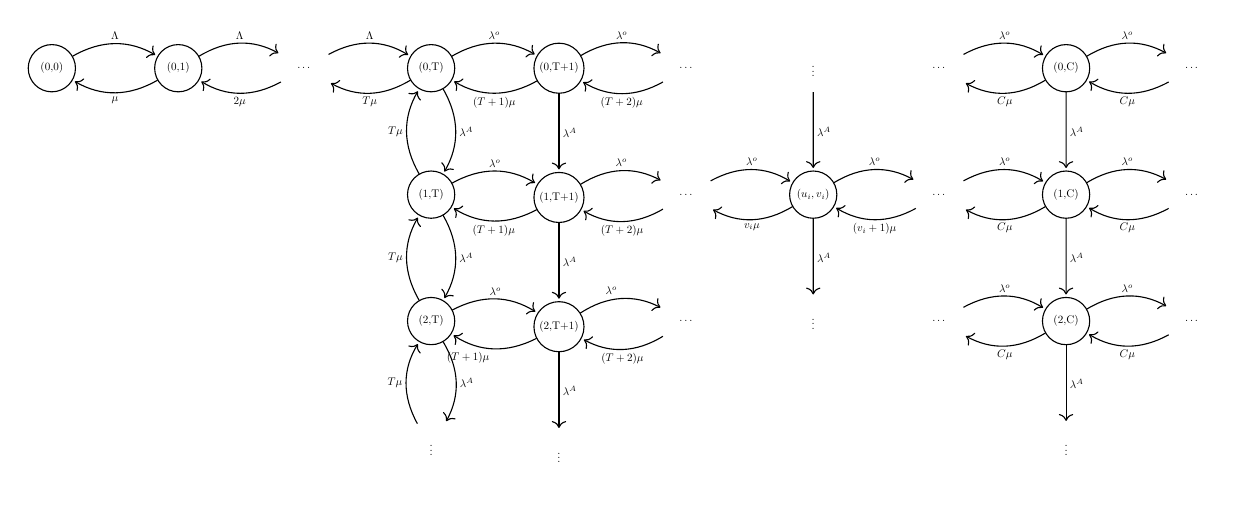
\begin{tikzpicture}[-, node distance = 1cm, auto, every node/.style={scale=0.4}]

        % Variables
        \tikzmath{
            let \altdist = 1cm;
            let \minsz = 1.5cm;
        }

        % First Line
        \node[state, minimum size=1.5cm] (zero) {(0,0)};
        \node[state, minimum size=1.5cm,  right=of zero] (one) {(0,1)};
        \node[draw=none, minimum size=1.5cm, right=of one] (two) {\dots};
        \node[state, minimum size=1.5cm, right=of two] (three) {(0,T)};
        \node[state, node distance = \altdist, minimum size=\minsz, right=of three] (four) {(0,T+1)};
        \node[draw=none, minimum size=\minsz, right=of four] (five) {\dots};
        \node[draw=none, minimum size=\minsz, right=of five] (six) {\vdots};
        \node[draw=none, minimum size=\minsz, right=of six] (seven) {\dots};
        \node[state, minimum size=\minsz, right=of seven] (eight) {(0,C)};
        \node[draw=none, minimum size=\minsz, right=of eight] (nine) {\dots};


        % Second Line
        \node[state, minimum size=\minsz, below=of three] (three_one) {(1,T)};
        \node[state, minimum size=\minsz, below=of four] (four_one) {(1,T+1)};
        \node[draw=none, minimum size=\minsz, below=of five] (five_one) {\dots};
        \node[state, node distance = \altdist, minimum size=\minsz, right=of five_one] (six_one) {\( (u_i, v_i) \)};
        \node[draw=none, minimum size=\minsz, right=of six_one] (seven_one) {\dots};
        \node[state, node distance = \altdist, minimum size=\minsz, right=of seven_one] (eight_one) {(1,C)};
        \node[draw=none, minimum size=\minsz, right=of eight_one] (nine_one) {\dots};
        

        % Third Line
        \node[state, minimum size=\minsz, below=of three_one] (three_two) {(2,T)};
        \node[state, minimum size=\minsz, below=of four_one] (four_two) {(2,T+1)};
        \node[draw=none, minimum size=\minsz, below=of five_one] (five_two) {\dots};
        \node[draw=none, node distance = \altdist, minimum size=\minsz, right=of five_two] (six_two) {\vdots};
        \node[draw=none, minimum size=\minsz, right=of six_two] (seven_two) {\dots};
        \node[state, node distance = \altdist, minimum size=\minsz, right=of seven_two] (eight_two) {(2,C)};
        \node[draw=none, minimum size=\minsz, right=of eight_two] (nine_two) {\dots};

        % Fourth line
        \node[draw=none, minimum size=\minsz, below=of three_two] (three_three) {\vdots};
        \node[draw=none, minimum size=\minsz, below=of four_two] (four_three) {\vdots};
        \node[draw=none, minimum size=\minsz, below=of five_two] (five_three) {};
        \node[draw=none, node distance = \altdist, minimum size=\minsz, right=of five_three] (six_three) {};
        \node[draw=none, node distance = \altdist, minimum size=\minsz, below=of eight_two] (eight_three) {\vdots};


        \draw[every loop]
            % First Horizontal Edges
            (zero) edge[bend left] node {\( \Lambda \)} (one)
            (one) edge[bend left] node {\( \mu \)} (zero)
            (one) edge[bend left] node {\( \Lambda \)} (two)
            (two) edge[bend left] node {\( 2 \mu \)} (one)
            (two) edge[bend left] node {\( \Lambda \)} (three)
            (three) edge[bend left] node {\( T \mu \)} (two)
            (three) edge[bend left] node {\( \lambda^o \)} (four)
            (four) edge[bend left] node {\( (T+1) \mu \)} (three)
            (four) edge[bend left] node {\( \lambda^o \)} (five)
            (five) edge[bend left] node {\( (T+2) \mu \)} (four)
            % (five) edge[bend left] node {\( \lambda^o \)} (six)
            % (six) edge[bend left] node [above] {\( C\mu \)} (five)
            % (six) edge[bend left] node {\( \lambda^o \)} (seven)
            % (seven) edge[bend left] node [above] {\( C\mu \)} (six)
            (seven) edge[bend left] node {\( \lambda^o \)} (eight)
            (eight) edge[bend left] node {\( C\mu \)} (seven)
            (eight) edge[bend left] node {\( \lambda^o \)} (nine)
            (nine) edge[bend left] node {\( C\mu \)} (eight)

            % Second Horizontal Edges
            (three_one) edge[bend left] node {\(\lambda^o\)} (four_one)
            (four_one) edge[bend left] node {\( (T+1) \mu \)} (three_one)
            (four_one) edge[bend left] node {\( \lambda^o \)} (five_one)
            (five_one) edge[bend left] node {\( (T+2) \mu \)} (four_one)
            (five_one) edge[bend left] node {\( \lambda^o \)} (six_one)
            (six_one) edge[bend left] node {\( v_i\mu \)} (five_one)
            (six_one) edge[bend left] node {\( \lambda^o \)} (seven_one)
            (seven_one) edge[bend left] node {\( (v_i+1)\mu \)} (six_one)
            (seven_one) edge[bend left] node {\( \lambda^o \)} (eight_one)
            (eight_one) edge[bend left] node {\( C\mu \)} (seven_one)
            (eight_one) edge[bend left] node {\( \lambda^o \)} (nine_one)
            (nine_one) edge[bend left] node {\( C\mu \)} (eight_one)

            % Third Horizontal Edges
            (three_two) edge[bend left] node {\( \lambda^o \)} (four_two)
            (four_two) edge[bend left] node {\( (T+1) \mu \)} (three_two)
            (four_two) edge[bend left] node {\( \lambda^o \)} (five_two)
            (five_two) edge[bend left] node {\( (T+2) \mu \)} (four_two)
            % (five_two) edge[bend left] node {\( \lambda^o \)} (six_two)
            % (six_two) edge[bend left] node [above] {\( C\mu \)} (five_two)
            % (six_two) edge[bend left] node {\( \lambda^o \)} (seven_two)
            % (seven_two) edge[bend left] node [above] {\( C\mu \)} (six_two)
            (seven_two) edge[bend left] node {\( \lambda^o \)} (eight_two)
            (eight_two) edge[bend left] node {\( C\mu \)} (seven_two)
            (eight_two) edge[bend left] node {\( \lambda^o \)} (nine_two)
            (nine_two) edge[bend left] node {\( C\mu \)} (eight_two)

            % First Vertical Edges
            (three) edge[bend left] node {\( \lambda^A \)} (three_one)
            (three_one) edge[bend left] node {\( T \mu \)} (three)
            (three_one) edge[bend left] node {\( \lambda^A \)} (three_two)
            (three_two) edge[bend left] node {\( T\mu \)} (three_one)
            (three_two) edge[bend left] node {\( \lambda^A \)} (three_three)
            (three_three) edge[bend left] node {\( T\mu \)} (three_two)

            % Second Vertical Edges
            (four) edge node {\( \lambda^A \)} (four_one)
            (four_one) edge node {\( \lambda^A \)} (four_two)
            (four_two) edge node {\( \lambda^A \)} (four_three)

            % Third Vertical Edges
            (six) edge node {\( \lambda^A \)} (six_one)
            (six_one) edge node {\( \lambda^A \)} (six_two)
            % (six_two) edge node {\( \lambda^A \)} (six_three)

            % Fourth Vertical Edges
            (eight) edge node {\( \lambda^A \)} (eight_one)
            (eight_one) edge node {\( \lambda^A \)} (eight_two)
            (eight_two) edge node {\( \lambda^A \)} (eight_three)
            ;       
    \end{tikzpicture}
    \caption{Markov chains} 
    \label{Markov_3}
\end{figure}


\begin{figure}
    \centering
    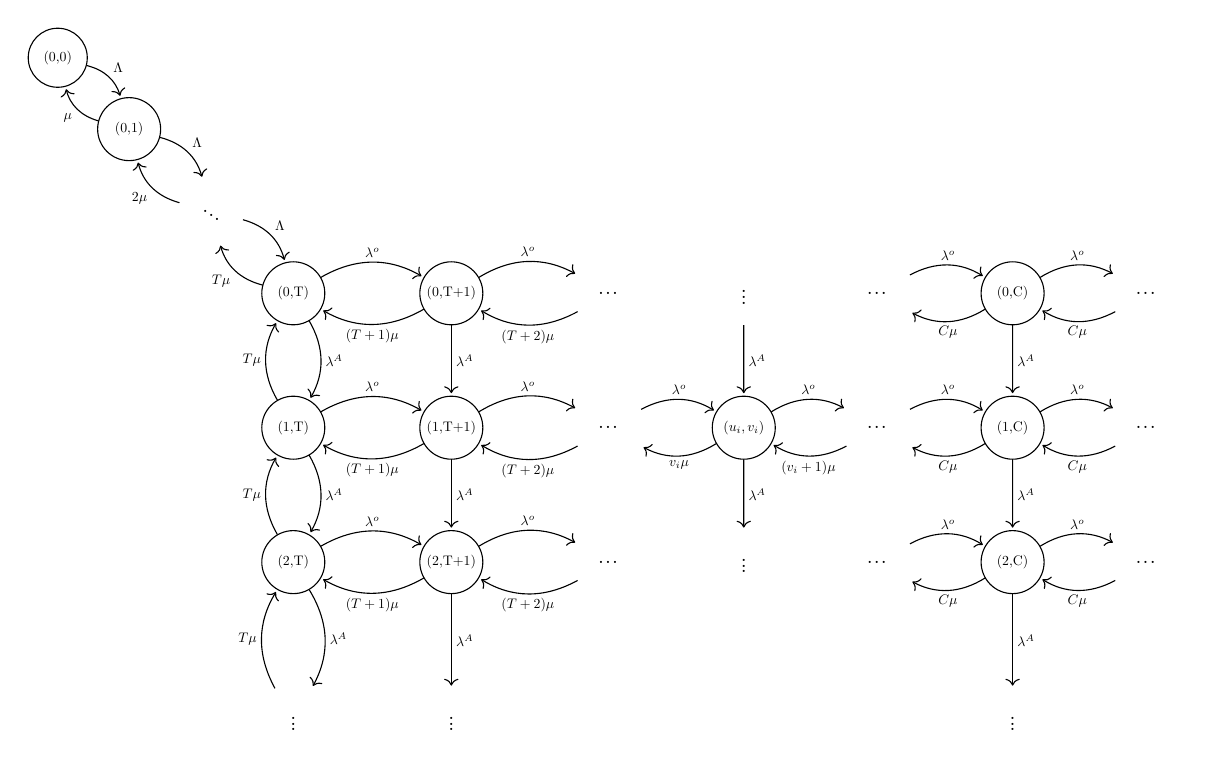
\begin{tikzpicture}[-, node distance = 0.9cm, auto, every node/.style={scale=0.5}]

        % Variables
        \tikzmath{
            let \initdist = 0.5cm;
            let \altdist = 1.2cm;
            let \minsz = 1.6cm;
            let \leftOne = -0.8;
            let \rightOne = 2.2;
            let \upOne = 0.8;
            let \downOne = -2.2;
            let \leftTwo = 2.25;
            let \rightTwo = 14.2;
            let \upTwo = -2.35;
            let \downTwo = -8.8;
        }

        % % Rectangle for S1
        % \draw[ultra thin, dashed] (\leftOne, \downOne) -- (\leftOne, \upOne);
        % \draw[ultra thin, dashed] (\leftOne, \upOne) -- (\rightOne, \upOne);
        % \draw[ultra thin, dashed] (\rightOne, \upOne) -- node {\Huge{\( \quad S_1 \)}}(\rightOne, \downOne);
        % \draw[ultra thin, dashed] (\rightOne, \downOne) -- (\leftOne, \downOne);

        % % Rectangle for S2
        % \draw[ultra thin, dashed] (\leftTwo, \downTwo) -- node {\Huge{\( S_2 \quad \)}}(\leftTwo, \upTwo);
        % \draw[ultra thin, dashed] (\leftTwo, \upTwo) -- (\rightTwo, \upTwo);
        % \draw[ultra thin, dashed] (\rightTwo, \upTwo) -- (\rightTwo, \downTwo);
        % \draw[ultra thin, dashed] (\rightTwo, \downTwo) -- (\leftTwo, \downTwo);

        % First Line
        \node[state, minimum size=1.5cm] (zero) {(0,0)};
        \node[state, node distance = \initdist, minimum size=\minsz, below right=of zero] (one) {(0,1)};
        \node[draw=none, node distance = \initdist, minimum size=\minsz, below right=of one] (two) {\textbf{\( \ddots \)}};
        \node[state, node distance = \initdist, minimum size=\minsz, below right=of two] (three) {(0,T)};
        \node[state, node distance = \altdist, minimum size=\minsz, right=of three] (four) {(0,T+1)};
        \node[draw=none, node distance = \altdist, minimum size=\minsz, right=of four] (five) {\textbf{\dots}};
        \node[draw=none, minimum size=\minsz, right=of five] (six) {\textbf{\vdots}};
        \node[draw=none, minimum size=\minsz, right=of six] (seven) {\textbf{\dots}};
        \node[state, minimum size=\minsz, right=of seven] (eight) {(0,C)};
        \node[draw=none, minimum size=\minsz, right=of eight] (nine) {\textbf{\dots}};


        % Second Line
        \node[state, minimum size=\minsz, below=of three] (three_one) {(1,T)};
        \node[state, minimum size=\minsz, below=of four] (four_one) {(1,T+1)};
        \node[draw=none, minimum size=\minsz, below=of five] (five_one) {\textbf{\dots}};
        \node[state, minimum size=\minsz, right=of five_one] (six_one) {\( (u_i, v_i) \)};
        \node[draw=none, minimum size=\minsz, right=of six_one] (seven_one) {\textbf{\dots}};
        \node[state, minimum size=\minsz, right=of seven_one] (eight_one) {(1,C)};
        \node[draw=none, minimum size=\minsz, right=of eight_one] (nine_one) {\textbf{\dots}};
        

        % Third Line
        \node[state, minimum size=\minsz, below=of three_one] (three_two) {(2,T)};
        \node[state, minimum size=\minsz, below=of four_one] (four_two) {(2,T+1)};
        \node[draw=none, minimum size=\minsz, below=of five_one] (five_two) {\textbf{\dots}};
        \node[draw=none, minimum size=\minsz, right=of five_two] (six_two) {\textbf{\vdots}};
        \node[draw=none, minimum size=\minsz, right=of six_two] (seven_two) {\textbf{\dots}};
        \node[state, minimum size=\minsz, right=of seven_two] (eight_two) {(2,C)};
        \node[draw=none, minimum size=\minsz, right=of eight_two] (nine_two) {\textbf{\dots}};

        % Fourth line
        \node[draw=none, node distance = \altdist, minimum size=\minsz, below=of three_two] (three_three) {\textbf{\vdots}};
        \node[draw=none, node distance = \altdist, minimum size=\minsz, below=of four_two] (four_three) {\textbf{\vdots}};
        \node[draw=none, node distance = \altdist, minimum size=\minsz, below=of five_two] (five_three) {};
        \node[draw=none, node distance = \altdist, minimum size=\minsz, below=of six_two] (six_three) {};
        \node[draw=none, node distance = \altdist, minimum size=\minsz, below=of eight_two] (eight_three) {\textbf{\vdots}};


        \draw[every loop]
            % First Horizontal Edges
            (zero) edge[bend left] node {\( \Lambda \)} (one)
            (one) edge[bend left] node {\( \mu \)} (zero)
            (one) edge[bend left] node {\( \Lambda \)} (two)
            (two) edge[bend left] node {\( 2 \mu \)} (one)
            (two) edge[bend left] node {\( \Lambda \)} (three)
            (three) edge[bend left] node {\( T \mu \)} (two)
            (three) edge[bend left] node {\( \lambda^o \)} (four)
            (four) edge[bend left] node {\( (T+1) \mu \)} (three)
            (four) edge[bend left] node {\( \lambda^o \)} (five)
            (five) edge[bend left] node {\( (T+2) \mu \)} (four)
            % (five) edge[bend left] node {\( \lambda^o \)} (six)
            % (six) edge[bend left] node [above] {\( C\mu \)} (five)
            % (six) edge[bend left] node {\( \lambda^o \)} (seven)
            % (seven) edge[bend left] node [above] {\( C\mu \)} (six)
            (seven) edge[bend left] node {\( \lambda^o \)} (eight)
            (eight) edge[bend left] node {\( C\mu \)} (seven)
            (eight) edge[bend left] node {\( \lambda^o \)} (nine)
            (nine) edge[bend left] node {\( C\mu \)} (eight)

            % Second Horizontal Edges
            (three_one) edge[bend left] node {\( \lambda^o \)} (four_one)
            (four_one) edge[bend left] node {\( (T+1) \mu \)} (three_one)
            (four_one) edge[bend left] node {\( \lambda^o \)} (five_one)
            (five_one) edge[bend left] node {\( (T+2) \mu \)} (four_one)
            (five_one) edge[bend left] node {\( \lambda^o \)} (six_one)
            (six_one) edge[bend left] node {\( v_i\mu \)} (five_one)
            (six_one) edge[bend left] node {\( \lambda^o \)} (seven_one)
            (seven_one) edge[bend left] node {\( (v_i+1)\mu \)} (six_one)
            (seven_one) edge[bend left] node {\( \lambda^o \)} (eight_one)
            (eight_one) edge[bend left] node {\( C\mu \)} (seven_one)
            (eight_one) edge[bend left] node {\( \lambda^o \)} (nine_one)
            (nine_one) edge[bend left] node {\( C\mu \)} (eight_one)

            % Third Horizontal Edges
            (three_two) edge[bend left] node {\( \lambda^o \)} (four_two)
            (four_two) edge[bend left] node [below] {\( (T+1) \mu \)} (three_two)
            (four_two) edge[bend left] node {\( \lambda^o \)} (five_two)
            (five_two) edge[bend left] node {\( (T+2) \mu \)} (four_two)
            % (five_two) edge[bend left] node {\( \lambda^o \)} (six_two)
            % (six_two) edge[bend left] node [above] {\( C\mu \)} (five_two)
            % (six_two) edge[bend left] node {\( \lambda^o \)} (seven_two)
            % (seven_two) edge[bend left] node [above] {\( C\mu \)} (six_two)
            (seven_two) edge[bend left] node {\( \lambda^o \)} (eight_two)
            (eight_two) edge[bend left] node {\( C\mu \)} (seven_two)
            (eight_two) edge[bend left] node {\( \lambda^o \)} (nine_two)
            (nine_two) edge[bend left] node {\( C\mu \)} (eight_two)

            % First Vertical Edges
            (three) edge[bend left] node {\( \lambda^A \)} (three_one)
            (three_one) edge[bend left] node {\( T \mu \)} (three)
            (three_one) edge[bend left] node {\( \lambda^A \)} (three_two)
            (three_two) edge[bend left] node {\( T\mu \)} (three_one)
            (three_two) edge[bend left] node {\( \lambda^A \)} (three_three)
            (three_three) edge[bend left] node {\( T\mu \)} (three_two)

            % Second Vertical Edges
            (four) edge node {\( \lambda^A \)} (four_one)
            (four_one) edge node {\( \lambda^A \)} (four_two)
            (four_two) edge node {\( \lambda^A \)} (four_three)

            % Third Vertical Edges
            (six) edge node {\( \lambda^A \)} (six_one)
            (six_one) edge node {\( \lambda^A \)} (six_two)
            % (six_two) edge node {\( \lambda^A \)} (six_three)

            % Fourth Vertical Edges
            (eight) edge node {\( \lambda^A \)} (eight_one)
            (eight_one) edge node {\( \lambda^A \)} (eight_two)
            (eight_two) edge node {\( \lambda^A \)} (eight_three)
            ;       
    \end{tikzpicture}
    \caption{Markov chains} 
    \label{Markov_4}
\end{figure}




\begin{figure}
    \centering
    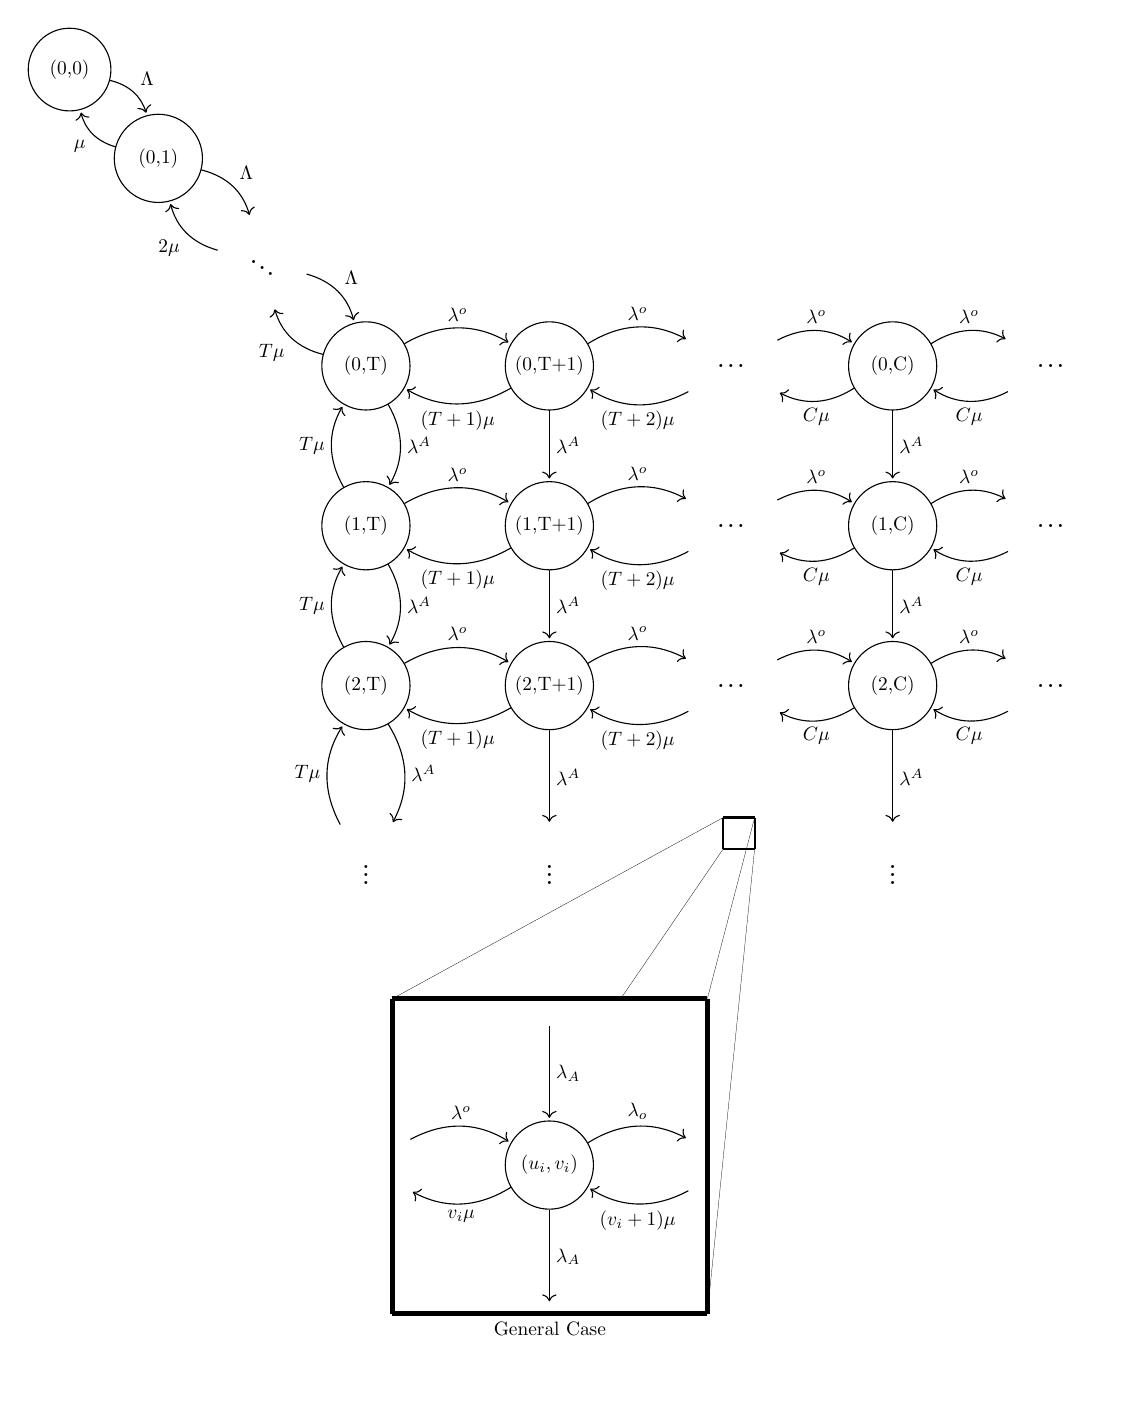
\begin{tikzpicture}[-, node distance = 0.9cm, auto, every node/.style={scale=0.7}]

        % Markov chain variables
        \tikzmath{
            let \initdist = 0.5cm;
            let \altdist = 1.2cm;
            let \minsz = 1.6cm;
        }

        % S_1 and S_2 rectangles
        \tikzmath{
            let \leftOne = -0.8;
            let \rightOne = 2.7;
            let \upOne = 0.8;
            let \downOne = -2.7;
            let \leftTwo = 2.8;
            let \rightTwo = 13;
            let \upTwo = -2.95;
            let \downTwo = -16.4;
        }

        % General case variables
        \tikzmath{
            let \GCsmallx = 8.3;
            let \GCsmally = -9.5;
            let \GCbigx = 4.1;
            let \GCbigy = -11.8;
        }

        % % Rectangle for S1
        % \draw[ultra thin, dashed] (\leftOne, \downOne) -- (\leftOne, \upOne);
        % \draw[ultra thin, dashed] (\leftOne, \upOne) -- (\rightOne, \upOne);
        % \draw[ultra thin, dashed] (\rightOne, \upOne) -- node {\Huge{\( \quad S_1 \)}}(\rightOne, \downOne);
        % \draw[ultra thin, dashed] (\rightOne, \downOne) -- (\leftOne, \downOne);

        % % Rectangle for S2
        % \draw[ultra thin, dashed] (\leftTwo, \downTwo) -- node {\Huge{\( S_2 \quad \)}}(\leftTwo, \upTwo);
        % \draw[ultra thin, dashed] (\leftTwo, \upTwo) -- (\rightTwo, \upTwo);
        % \draw[ultra thin, dashed] (\rightTwo, \upTwo) -- (\rightTwo, \downTwo);
        % \draw[ultra thin, dashed] (\rightTwo, \downTwo) -- (\leftTwo, \downTwo);

        % Small square of general case
        \draw [thick] (\GCsmallx, \GCsmally) -- node {} (\GCsmallx + 0.4, \GCsmally);
        \draw [thick] (\GCsmallx + 0.4, \GCsmally) -- node {} (\GCsmallx + 0.4, \GCsmally - 0.4);
        \draw [thick] (\GCsmallx + 0.4, \GCsmally - 0.4) -- node {} (\GCsmallx, \GCsmally - 0.4);
        \draw [thick] (\GCsmallx, \GCsmally - 0.4) -- node {} (\GCsmallx, \GCsmally);


        % Dashed lines to from small square to big one 
        \draw [ultra thin] (\GCsmallx, \GCsmally) -- node {} (\GCbigx, \GCbigy);
        \draw [ultra thin] (\GCsmallx + 0.4, \GCsmally) -- node {} (\GCbigx + 4, \GCbigy);
        \draw [ultra thin] (\GCsmallx, \GCsmally - 0.4) -- node {} (7, \GCbigy);
        \draw [ultra thin] (\GCsmallx + 0.4, \GCsmally - 0.4) -- node {} (\GCbigx + 4, \GCbigy - 4);
        
        % Big Square of general case
        \draw [ultra thick] (\GCbigx, \GCbigy) -- node {} (\GCbigx + 4, \GCbigy);
        \draw [ultra thick] (\GCbigx + 4, \GCbigy) -- node {} (\GCbigx + 4, \GCbigy - 4);
        \draw [ultra thick] (\GCbigx + 4, \GCbigy - 4) -- node {General Case} (\GCbigx, \GCbigy - 4);
        \draw [ultra thick] (\GCbigx, \GCbigy - 4) -- node {} (\GCbigx, \GCbigy);

        % First Line
        \node[state, minimum size=1.5cm] (zero) {(0,0)};
        \node[state, node distance = \initdist, minimum size=\minsz, below right=of zero] (one) {(0,1)};
        \node[draw=none, node distance = \initdist, minimum size=\minsz, below right=of one] (two) {\textbf{\( \ddots \)}};
        \node[state, node distance = \initdist, minimum size=\minsz, below right=of two] (three) {(0,T)};
        \node[state, node distance = \altdist, minimum size=\minsz, right=of three] (four) {(0,T+1)};
        \node[draw=none, node distance = \altdist, minimum size=\minsz, right=of four] (five) {\textbf{\dots}};
        \node[state, minimum size=\minsz, right=of five] (six) {(0,C)};
        \node[draw=none, minimum size=\minsz, right=of six] (seven) {\textbf{\dots}};

        % Second Line
        \node[state, minimum size=\minsz, below=of three] (three_one) {(1,T)};
        \node[state, minimum size=\minsz, below=of four] (four_one) {(1,T+1)};
        \node[draw=none, minimum size=\minsz, below=of five] (five_one) {\textbf{\dots}};
        \node[state, minimum size=\minsz, right=of five_one] (six_one) {(1,C)};
        \node[draw=none, minimum size=\minsz, right=of six_one] (seven_one) {\textbf{\dots}};
        
        % Third Line
        \node[state, minimum size=\minsz, below=of three_one] (three_two) {(2,T)};
        \node[state, minimum size=\minsz, below=of four_one] (four_two) {(2,T+1)};
        \node[draw=none, minimum size=\minsz, below=of five_one] (five_two) {\textbf{\dots}};
        \node[state, minimum size=\minsz, right=of five_two] (six_two) {(2,C)};
        \node[draw=none, minimum size=\minsz, right=of six_two] (seven_two) {\textbf{\dots}};

        % Fourth line
        \node[draw=none, node distance = \altdist, minimum size=\minsz, below=of three_two] (three_three) {\textbf{\vdots}};
        \node[draw=none, node distance = \altdist, minimum size=\minsz, below=of four_two] (four_three) {\textbf{\vdots}};
        \node[draw=none, node distance = 2cm, minimum size=\minsz, below=of five_two] (five_three) {};
        \node[draw=none, node distance = \altdist, minimum size=\minsz, below=of six_two] (six_three) {\textbf{\vdots}};

        % Fifth line
        % \node[state, node distance = \altdist, minimum size=\minsz, below=of five_three] (general_case_mid) {\( (u_i, v_i) \)};
        \node[draw=none, node distance = 0.3cm, minimum size=\minsz, below=of four_three] (general_case_up) {};
        \node[state, node distance = \altdist, minimum size=\minsz, below=of general_case_up] (general_case_mid) {\( (u_i, v_i) \)};

        \node[draw=none, node distance = \altdist, minimum size=\minsz, below=of general_case_mid] (general_case_down) {};
        \node[draw=none, node distance = \altdist, minimum size=\minsz, left=of general_case_mid] (general_case_left) {};
        \node[draw=none, node distance = \altdist, minimum size=\minsz, right=of general_case_mid] (general_case_right) {};

        \draw[every loop]
            % First Horizontal Edges
            (zero) edge[bend left] node {\( \Lambda \)} (one)
            (one) edge[bend left] node {\( \mu \)} (zero)
            (one) edge[bend left] node {\( \Lambda \)} (two)
            (two) edge[bend left] node {\( 2 \mu \)} (one)
            (two) edge[bend left] node {\( \Lambda \)} (three)
            (three) edge[bend left] node {\( T \mu \)} (two)
            (three) edge[bend left] node {\( \lambda^o \)} (four)
            (four) edge[bend left] node {\( (T+1) \mu \)} (three)
            (four) edge[bend left] node {\( \lambda^o \)} (five)
            (five) edge[bend left] node {\( (T+2) \mu \)} (four)
            (five) edge[bend left] node {\( \lambda^o \)} (six)
            (six) edge[bend left] node {\( C\mu \)} (five)
            (six) edge[bend left] node {\( \lambda^o \)} (seven)
            (seven) edge[bend left] node {\( C\mu \)} (six)

            % Second Horizontal Edges
            (three_one) edge[bend left] node {\( \lambda^o \)} (four_one)
            (four_one) edge[bend left] node {\( (T+1) \mu \)} (three_one)
            (four_one) edge[bend left] node {\( \lambda^o \)} (five_one)
            (five_one) edge[bend left] node {\( (T+2) \mu \)} (four_one)
            (five_one) edge[bend left] node {\( \lambda^o \)} (six_one)
            (six_one) edge[bend left] node {\( C\mu \)} (five_one)
            (six_one) edge[bend left] node {\( \lambda^o \)} (seven_one)
            (seven_one) edge[bend left] node {\( C\mu \)} (six_one)

            % Third Horizontal Edges
            (three_two) edge[bend left] node {\( \lambda^o \)} (four_two)
            (four_two) edge[bend left] node [below] {\( (T+1) \mu \)} (three_two)
            (four_two) edge[bend left] node {\( \lambda^o \)} (five_two)
            (five_two) edge[bend left] node {\( (T+2) \mu \)} (four_two)
            (five_two) edge[bend left] node {\( \lambda^o \)} (six_two)
            (six_two) edge[bend left] node {\( C\mu \)} (five_two)
            (six_two) edge[bend left] node {\( \lambda^o \)} (seven_two)
            (seven_two) edge[bend left] node {\( C\mu \)} (six_two)

            % First Vertical Edges
            (three) edge[bend left] node {\( \lambda^A \)} (three_one)
            (three_one) edge[bend left] node {\( T \mu \)} (three)
            (three_one) edge[bend left] node {\( \lambda^A \)} (three_two)
            (three_two) edge[bend left] node {\( T\mu \)} (three_one)
            (three_two) edge[bend left] node {\( \lambda^A \)} (three_three)
            (three_three) edge[bend left] node {\( T\mu \)} (three_two)

            % Second Vertical Edges
            (four) edge node {\( \lambda^A \)} (four_one)
            (four_one) edge node {\( \lambda^A \)} (four_two)
            (four_two) edge node {\( \lambda^A \)} (four_three)

            % Fourth Vertical Edges
            (six) edge node {\( \lambda^A \)} (six_one)
            (six_one) edge node {\( \lambda^A \)} (six_two)
            (six_two) edge node {\( \lambda^A \)} (six_three)

            % General Case
            (general_case_left) edge[bend left] node {\( \lambda^o \)} (general_case_mid)
            (general_case_mid) edge[bend left] node {\( v_i \mu \)} (general_case_left)
            (general_case_right) edge[bend left] node {\( (v_i +1) \mu \)} (general_case_mid)
            (general_case_mid) edge[bend left] node {\( \lambda_o \)} (general_case_right)
            % (five_three) edge node {\( \lambda_A \)} (general_case_mid)
            (general_case_up) edge node {\( \lambda_A \)} (general_case_mid)
            (general_case_mid) edge node {\( \lambda_A \)} (general_case_down)
            ;
    \end{tikzpicture}
    \caption{Markov chain} 
    \label{Markov_5}
\end{figure}


\newpage
\section{Figures that might be useful}
\begin{figure}[h]
    \centering
    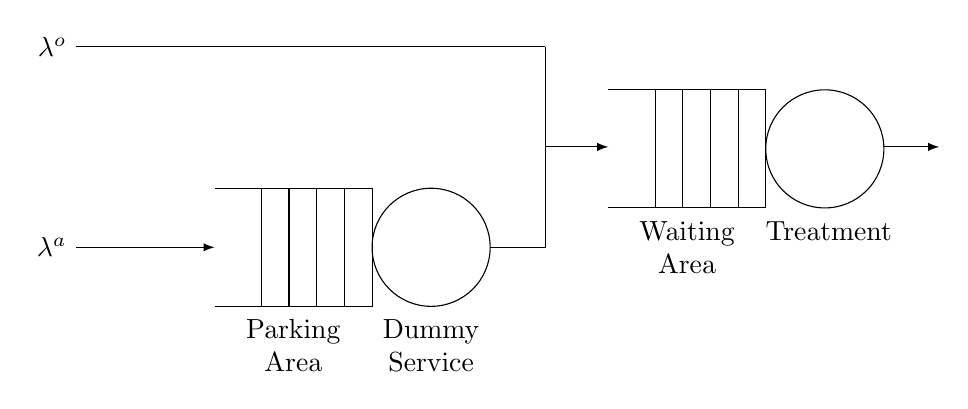
\begin{tikzpicture}[>=latex]
        % the rectangle with vertical rules (Queue 1)
        \draw (0,0) -- ++(2cm,0) -- ++(0,-1.5cm) -- ++(-2cm,0);
        \foreach \i in {1,...,4}
        \draw (2cm-\i*10pt,0) -- +(0,-1.5cm);
        
        % the circle (Queue 1)
        \draw (2.75,-0.75cm) circle [radius=0.75cm];

        % the rectangle with vertical rules (Queue 2)
        \draw (5,1.25) -- ++(2cm,0) -- ++(0,-1.5cm) -- ++(-2cm,0);
        \foreach \i in {1,...,4}
        \draw (7cm-\i*10pt,1.25) -- +(0,-1.5cm);

        % the circle (Queue 2)
        \draw (7.75,0.5) circle [radius=0.75cm];

        % the arrows and labels (Queue 1+2)
        \draw[-] (3.5,-0.75) -- +(20pt,0);
        \draw[<-] (0,-0.75) -- +(-50pt,0) node[left] {\( \lambda^a \)};
        \draw[->] (8.5,0.525) -- +(20pt,0);
        \node[align=center] at (1cm,-2cm) {Parking \\ Area};
        \node[align=center] at (2.75cm,-2cm) {Dummy \\ Service};
        \node[align=center] at (6cm,-0.75cm) {Waiting \\ Area};
        \node[align=center] at (7.8cm,-0.75cm) {Treatment \\ };
        
        \draw (4.2, 1.8) -- +(-169.5pt,0) node[left] {\( \lambda^o \)};
        \draw (4.2, 1.8) -- (4.2, -0.75);
        \draw[->] (4.2, 0.525) -- (5, 0.525);

    \end{tikzpicture}
\end{figure}


\begin{figure}
    \centering
    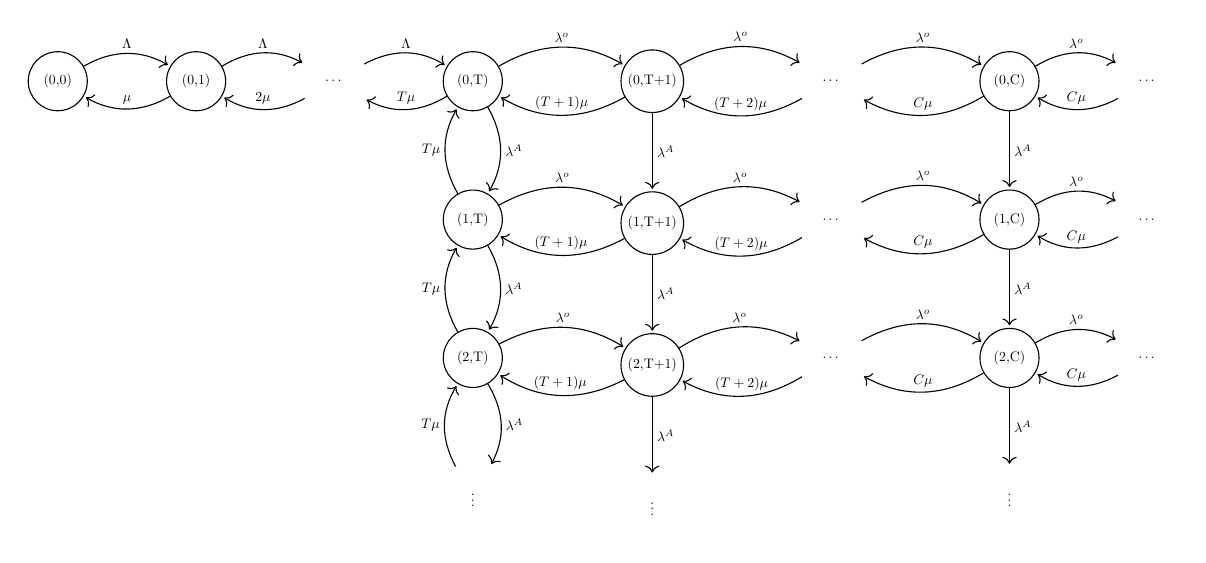
\begin{tikzpicture}[-, node distance = 1cm, auto, every node/.style={scale=0.5}]

        % Variables
        \tikzmath{
            let \altdist = 1.5cm;
            let \minsz = 1.5cm;
        }

        % First Line
        \node[state, minimum size=1.5cm] (zero) {(0,0)};
        \node[state, minimum size=1.5cm,  right=of zero] (one) {(0,1)};
        \node[draw=none, minimum size=1.5cm, right=of one] (two) {\dots};
        \node[state, minimum size=1.5cm, right=of two] (three) {(0,T)};
        \node[state, node distance = \altdist, minimum size=\minsz, right=of three] (four) {(0,T+1)};
        \node[draw=none, node distance = \altdist, minimum size=\minsz, right=of four] (five) {\dots};
        \node[state, node distance = \altdist, minimum size=\minsz, right=of five] (six) {(0,C)};
        \node[draw=none, minimum size=\minsz, right=of six] (seven) {\dots};

        % Second Line
        \node[state, minimum size=\minsz, below=of three] (three_one) {(1,T)};
        \node[state, minimum size=\minsz, below=of four] (four_one) {(1,T+1)};
        \node[draw=none, minimum size=\minsz, below=of five] (five_one) {\dots};
        \node[state, node distance = \altdist, minimum size=\minsz, right=of five_one] (six_one) {(1,C)};
        \node[draw=none, minimum size=\minsz, right=of six_one] (seven_one) {\dots};

        % Third Line
        \node[state, minimum size=\minsz, below=of three_one] (three_two) {(2,T)};
        \node[state, minimum size=\minsz, below=of four_one] (four_two) {(2,T+1)};
        \node[draw=none, minimum size=\minsz, below=of five_one] (five_two) {\dots};
        \node[state, node distance = \altdist, minimum size=\minsz, right=of five_two] (six_two) {(2,C)};
        \node[draw=none, minimum size=\minsz, right=of six_two] (seven_two) {\dots};

        % Fourth line
        \node[draw=none, minimum size=\minsz, below=of three_two] (three_three) {\vdots};
        \node[draw=none, minimum size=\minsz, below=of four_two] (four_three) {\vdots};
        \node[draw=none, minimum size=\minsz, below=of five_two] (five_three) {};
        \node[draw=none, node distance = \altdist, minimum size=\minsz, right=of five_three] (six_three) {\vdots};

        \draw[every loop]
            % First Horizontal Edges
            (zero) edge[bend left] node {\( \Lambda \)} (one)
            (one) edge[bend left] node [above] {\( \mu \)} (zero)
            (one) edge[bend left] node {\( \Lambda \)} (two)
            (two) edge[bend left] node [above] {\( 2 \mu \)} (one)
            (two) edge[bend left] node {\( \Lambda \)} (three)
            (three) edge[bend left] node [above] {\( T \mu \)} (two)
            (three) edge[bend left] node {\( \lambda^o \)} (four)
            (four) edge[bend left] node [above] {\( (T+1) \mu \)} (three)
            (four) edge[bend left] node {\( \lambda^o \)} (five)
            (five) edge[bend left] node [above] {\( (T+2) \mu \)} (four)
            (five) edge[bend left] node {\( \lambda^o \)} (six)
            (six) edge[bend left] node [above] {\( C\mu \)} (five)
            (six) edge[bend left] node {\( \lambda^o \)} (seven)
            (seven) edge[bend left] node [above] {\( C\mu \)} (six)

            % Second Horizontal Edges
            (three_one) edge[bend left] node {\( \lambda^o \)} (four_one)
            (four_one) edge[bend left] node [above] {\( (T+1) \mu \)} (three_one)
            (four_one) edge[bend left] node {\( \lambda^o \)} (five_one)
            (five_one) edge[bend left] node [above] {\( (T+2) \mu \)} (four_one)
            (five_one) edge[bend left] node {\( \lambda^o \)} (six_one)
            (six_one) edge[bend left] node [above] {\( C\mu \)} (five_one)
            (six_one) edge[bend left] node {\( \lambda^o \)} (seven_one)
            (seven_one) edge[bend left] node [above] {\( C\mu \)} (six_one)

            % Third Horizontal Edges
            (three_two) edge[bend left] node {\( \lambda^o \)} (four_two)
            (four_two) edge[bend left] node [above] {\( (T+1) \mu \)} (three_two)
            (four_two) edge[bend left] node {\( \lambda^o \)} (five_two)
            (five_two) edge[bend left] node [above] {\( (T+2) \mu \)} (four_two)
            (five_two) edge[bend left] node {\( \lambda^o \)} (six_two)
            (six_two) edge[bend left] node [above] {\( C\mu \)} (five_two)
            (six_two) edge[bend left] node {\( \lambda^o \)} (seven_two)
            (seven_two) edge[bend left] node [above] {\( C\mu \)} (six_two)

            % First Vertical Edges
            (three) edge[bend left] node {\( \lambda^A \)} (three_one)
            (three_one) edge[bend left] node {\( T \mu \)} (three)
            (three_one) edge[bend left] node {\( \lambda^A \)} (three_two)
            (three_two) edge[bend left] node {\( T\mu \)} (three_one)
            (three_two) edge[bend left] node {\( \lambda^A \)} (three_three)
            (three_three) edge[bend left] node {\( T\mu \)} (three_two)

            % Second Vertical Edges
            (four) edge node {\( \lambda^A \)} (four_one)
            (four_one) edge node {\( \lambda^A \)} (four_two)
            (four_two) edge node {\( \lambda^A \)} (four_three)

            %Third Vertical Edges
            (six) edge node {\( \lambda^A \)} (six_one)
            (six_one) edge node {\( \lambda^A \)} (six_two)
            (six_two) edge node {\( \lambda^A \)} (six_three)
            ;       
    \end{tikzpicture}
    \caption{Markov chains} 
    \label{Markov_2}
\end{figure}



\begin{figure}
    \centering
    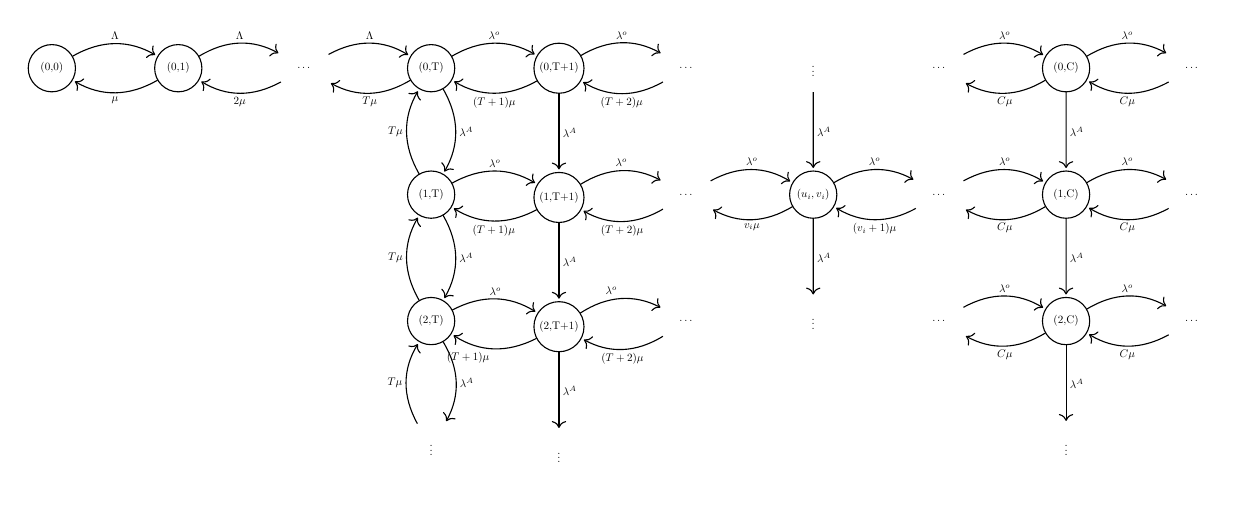
\begin{tikzpicture}[-, node distance = 1cm, auto, every node/.style={scale=0.4}]

        % Variables
        \tikzmath{
            let \altdist = 1cm;
            let \minsz = 1.5cm;
        }

        % First Line
        \node[state, minimum size=1.5cm] (zero) {(0,0)};
        \node[state, minimum size=1.5cm,  right=of zero] (one) {(0,1)};
        \node[draw=none, minimum size=1.5cm, right=of one] (two) {\dots};
        \node[state, minimum size=1.5cm, right=of two] (three) {(0,T)};
        \node[state, node distance = \altdist, minimum size=\minsz, right=of three] (four) {(0,T+1)};
        \node[draw=none, minimum size=\minsz, right=of four] (five) {\dots};
        \node[draw=none, minimum size=\minsz, right=of five] (six) {\vdots};
        \node[draw=none, minimum size=\minsz, right=of six] (seven) {\dots};
        \node[state, minimum size=\minsz, right=of seven] (eight) {(0,C)};
        \node[draw=none, minimum size=\minsz, right=of eight] (nine) {\dots};


        % Second Line
        \node[state, minimum size=\minsz, below=of three] (three_one) {(1,T)};
        \node[state, minimum size=\minsz, below=of four] (four_one) {(1,T+1)};
        \node[draw=none, minimum size=\minsz, below=of five] (five_one) {\dots};
        \node[state, node distance = \altdist, minimum size=\minsz, right=of five_one] (six_one) {\( (u_i, v_i) \)};
        \node[draw=none, minimum size=\minsz, right=of six_one] (seven_one) {\dots};
        \node[state, node distance = \altdist, minimum size=\minsz, right=of seven_one] (eight_one) {(1,C)};
        \node[draw=none, minimum size=\minsz, right=of eight_one] (nine_one) {\dots};
        

        % Third Line
        \node[state, minimum size=\minsz, below=of three_one] (three_two) {(2,T)};
        \node[state, minimum size=\minsz, below=of four_one] (four_two) {(2,T+1)};
        \node[draw=none, minimum size=\minsz, below=of five_one] (five_two) {\dots};
        \node[draw=none, node distance = \altdist, minimum size=\minsz, right=of five_two] (six_two) {\vdots};
        \node[draw=none, minimum size=\minsz, right=of six_two] (seven_two) {\dots};
        \node[state, node distance = \altdist, minimum size=\minsz, right=of seven_two] (eight_two) {(2,C)};
        \node[draw=none, minimum size=\minsz, right=of eight_two] (nine_two) {\dots};

        % Fourth line
        \node[draw=none, minimum size=\minsz, below=of three_two] (three_three) {\vdots};
        \node[draw=none, minimum size=\minsz, below=of four_two] (four_three) {\vdots};
        \node[draw=none, minimum size=\minsz, below=of five_two] (five_three) {};
        \node[draw=none, node distance = \altdist, minimum size=\minsz, right=of five_three] (six_three) {};
        \node[draw=none, node distance = \altdist, minimum size=\minsz, below=of eight_two] (eight_three) {\vdots};


        \draw[every loop]
            % First Horizontal Edges
            (zero) edge[bend left] node {\( \Lambda \)} (one)
            (one) edge[bend left] node {\( \mu \)} (zero)
            (one) edge[bend left] node {\( \Lambda \)} (two)
            (two) edge[bend left] node {\( 2 \mu \)} (one)
            (two) edge[bend left] node {\( \Lambda \)} (three)
            (three) edge[bend left] node {\( T \mu \)} (two)
            (three) edge[bend left] node {\( \lambda^o \)} (four)
            (four) edge[bend left] node {\( (T+1) \mu \)} (three)
            (four) edge[bend left] node {\( \lambda^o \)} (five)
            (five) edge[bend left] node {\( (T+2) \mu \)} (four)
            % (five) edge[bend left] node {\( \lambda^o \)} (six)
            % (six) edge[bend left] node [above] {\( C\mu \)} (five)
            % (six) edge[bend left] node {\( \lambda^o \)} (seven)
            % (seven) edge[bend left] node [above] {\( C\mu \)} (six)
            (seven) edge[bend left] node {\( \lambda^o \)} (eight)
            (eight) edge[bend left] node {\( C\mu \)} (seven)
            (eight) edge[bend left] node {\( \lambda^o \)} (nine)
            (nine) edge[bend left] node {\( C\mu \)} (eight)

            % Second Horizontal Edges
            (three_one) edge[bend left] node {\(\lambda^o\)} (four_one)
            (four_one) edge[bend left] node {\( (T+1) \mu \)} (three_one)
            (four_one) edge[bend left] node {\( \lambda^o \)} (five_one)
            (five_one) edge[bend left] node {\( (T+2) \mu \)} (four_one)
            (five_one) edge[bend left] node {\( \lambda^o \)} (six_one)
            (six_one) edge[bend left] node {\( v_i\mu \)} (five_one)
            (six_one) edge[bend left] node {\( \lambda^o \)} (seven_one)
            (seven_one) edge[bend left] node {\( (v_i+1)\mu \)} (six_one)
            (seven_one) edge[bend left] node {\( \lambda^o \)} (eight_one)
            (eight_one) edge[bend left] node {\( C\mu \)} (seven_one)
            (eight_one) edge[bend left] node {\( \lambda^o \)} (nine_one)
            (nine_one) edge[bend left] node {\( C\mu \)} (eight_one)

            % Third Horizontal Edges
            (three_two) edge[bend left] node {\( \lambda^o \)} (four_two)
            (four_two) edge[bend left] node {\( (T+1) \mu \)} (three_two)
            (four_two) edge[bend left] node {\( \lambda^o \)} (five_two)
            (five_two) edge[bend left] node {\( (T+2) \mu \)} (four_two)
            % (five_two) edge[bend left] node {\( \lambda^o \)} (six_two)
            % (six_two) edge[bend left] node [above] {\( C\mu \)} (five_two)
            % (six_two) edge[bend left] node {\( \lambda^o \)} (seven_two)
            % (seven_two) edge[bend left] node [above] {\( C\mu \)} (six_two)
            (seven_two) edge[bend left] node {\( \lambda^o \)} (eight_two)
            (eight_two) edge[bend left] node {\( C\mu \)} (seven_two)
            (eight_two) edge[bend left] node {\( \lambda^o \)} (nine_two)
            (nine_two) edge[bend left] node {\( C\mu \)} (eight_two)

            % First Vertical Edges
            (three) edge[bend left] node {\( \lambda^A \)} (three_one)
            (three_one) edge[bend left] node {\( T \mu \)} (three)
            (three_one) edge[bend left] node {\( \lambda^A \)} (three_two)
            (three_two) edge[bend left] node {\( T\mu \)} (three_one)
            (three_two) edge[bend left] node {\( \lambda^A \)} (three_three)
            (three_three) edge[bend left] node {\( T\mu \)} (three_two)

            % Second Vertical Edges
            (four) edge node {\( \lambda^A \)} (four_one)
            (four_one) edge node {\( \lambda^A \)} (four_two)
            (four_two) edge node {\( \lambda^A \)} (four_three)

            % Third Vertical Edges
            (six) edge node {\( \lambda^A \)} (six_one)
            (six_one) edge node {\( \lambda^A \)} (six_two)
            % (six_two) edge node {\( \lambda^A \)} (six_three)

            % Fourth Vertical Edges
            (eight) edge node {\( \lambda^A \)} (eight_one)
            (eight_one) edge node {\( \lambda^A \)} (eight_two)
            (eight_two) edge node {\( \lambda^A \)} (eight_three)
            ;       
    \end{tikzpicture}
    \caption{Markov chains} 
    \label{Markov_3}
\end{figure}


\begin{figure}
    \centering
    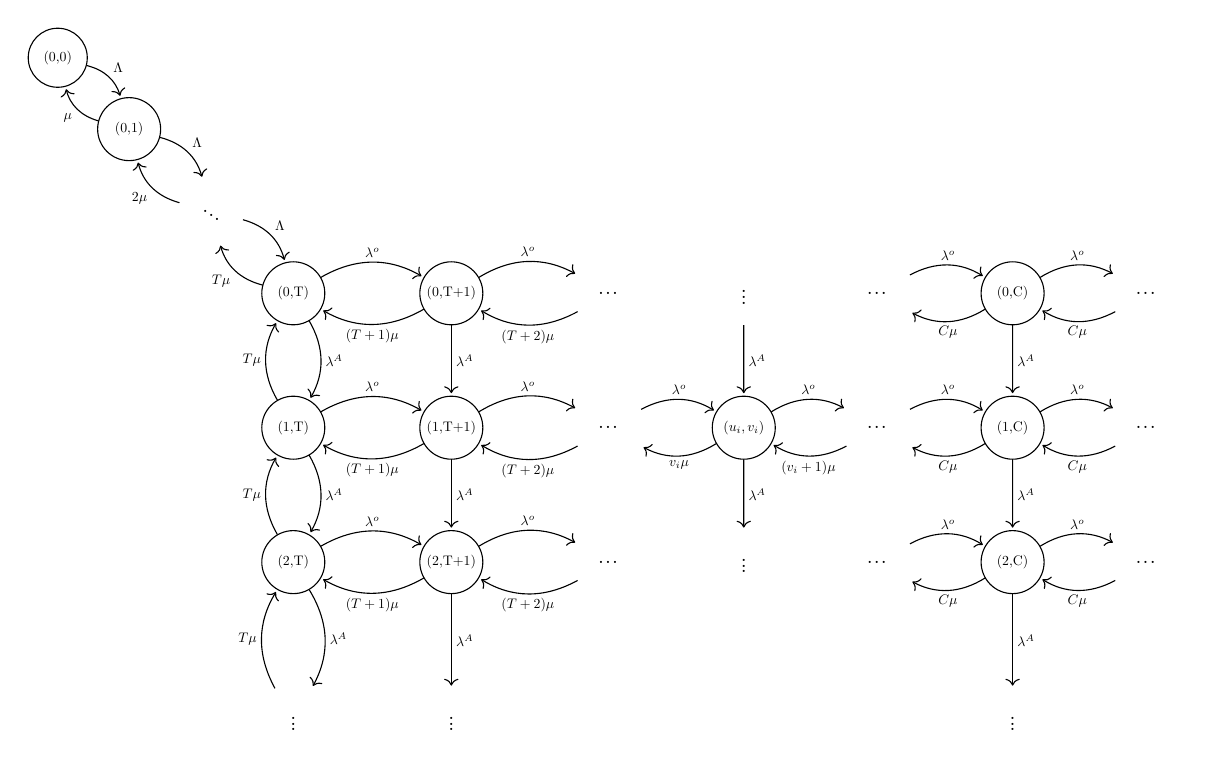
\begin{tikzpicture}[-, node distance = 0.9cm, auto, every node/.style={scale=0.5}]

        % Variables
        \tikzmath{
            let \initdist = 0.5cm;
            let \altdist = 1.2cm;
            let \minsz = 1.6cm;
            let \leftOne = -0.8;
            let \rightOne = 2.2;
            let \upOne = 0.8;
            let \downOne = -2.2;
            let \leftTwo = 2.25;
            let \rightTwo = 14.2;
            let \upTwo = -2.35;
            let \downTwo = -8.8;
        }

        % % Rectangle for S1
        % \draw[ultra thin, dashed] (\leftOne, \downOne) -- (\leftOne, \upOne);
        % \draw[ultra thin, dashed] (\leftOne, \upOne) -- (\rightOne, \upOne);
        % \draw[ultra thin, dashed] (\rightOne, \upOne) -- node {\Huge{\( \quad S_1 \)}}(\rightOne, \downOne);
        % \draw[ultra thin, dashed] (\rightOne, \downOne) -- (\leftOne, \downOne);

        % % Rectangle for S2
        % \draw[ultra thin, dashed] (\leftTwo, \downTwo) -- node {\Huge{\( S_2 \quad \)}}(\leftTwo, \upTwo);
        % \draw[ultra thin, dashed] (\leftTwo, \upTwo) -- (\rightTwo, \upTwo);
        % \draw[ultra thin, dashed] (\rightTwo, \upTwo) -- (\rightTwo, \downTwo);
        % \draw[ultra thin, dashed] (\rightTwo, \downTwo) -- (\leftTwo, \downTwo);

        % First Line
        \node[state, minimum size=1.5cm] (zero) {(0,0)};
        \node[state, node distance = \initdist, minimum size=\minsz, below right=of zero] (one) {(0,1)};
        \node[draw=none, node distance = \initdist, minimum size=\minsz, below right=of one] (two) {\textbf{\( \ddots \)}};
        \node[state, node distance = \initdist, minimum size=\minsz, below right=of two] (three) {(0,T)};
        \node[state, node distance = \altdist, minimum size=\minsz, right=of three] (four) {(0,T+1)};
        \node[draw=none, node distance = \altdist, minimum size=\minsz, right=of four] (five) {\textbf{\dots}};
        \node[draw=none, minimum size=\minsz, right=of five] (six) {\textbf{\vdots}};
        \node[draw=none, minimum size=\minsz, right=of six] (seven) {\textbf{\dots}};
        \node[state, minimum size=\minsz, right=of seven] (eight) {(0,C)};
        \node[draw=none, minimum size=\minsz, right=of eight] (nine) {\textbf{\dots}};


        % Second Line
        \node[state, minimum size=\minsz, below=of three] (three_one) {(1,T)};
        \node[state, minimum size=\minsz, below=of four] (four_one) {(1,T+1)};
        \node[draw=none, minimum size=\minsz, below=of five] (five_one) {\textbf{\dots}};
        \node[state, minimum size=\minsz, right=of five_one] (six_one) {\( (u_i, v_i) \)};
        \node[draw=none, minimum size=\minsz, right=of six_one] (seven_one) {\textbf{\dots}};
        \node[state, minimum size=\minsz, right=of seven_one] (eight_one) {(1,C)};
        \node[draw=none, minimum size=\minsz, right=of eight_one] (nine_one) {\textbf{\dots}};
        

        % Third Line
        \node[state, minimum size=\minsz, below=of three_one] (three_two) {(2,T)};
        \node[state, minimum size=\minsz, below=of four_one] (four_two) {(2,T+1)};
        \node[draw=none, minimum size=\minsz, below=of five_one] (five_two) {\textbf{\dots}};
        \node[draw=none, minimum size=\minsz, right=of five_two] (six_two) {\textbf{\vdots}};
        \node[draw=none, minimum size=\minsz, right=of six_two] (seven_two) {\textbf{\dots}};
        \node[state, minimum size=\minsz, right=of seven_two] (eight_two) {(2,C)};
        \node[draw=none, minimum size=\minsz, right=of eight_two] (nine_two) {\textbf{\dots}};

        % Fourth line
        \node[draw=none, node distance = \altdist, minimum size=\minsz, below=of three_two] (three_three) {\textbf{\vdots}};
        \node[draw=none, node distance = \altdist, minimum size=\minsz, below=of four_two] (four_three) {\textbf{\vdots}};
        \node[draw=none, node distance = \altdist, minimum size=\minsz, below=of five_two] (five_three) {};
        \node[draw=none, node distance = \altdist, minimum size=\minsz, below=of six_two] (six_three) {};
        \node[draw=none, node distance = \altdist, minimum size=\minsz, below=of eight_two] (eight_three) {\textbf{\vdots}};


        \draw[every loop]
            % First Horizontal Edges
            (zero) edge[bend left] node {\( \Lambda \)} (one)
            (one) edge[bend left] node {\( \mu \)} (zero)
            (one) edge[bend left] node {\( \Lambda \)} (two)
            (two) edge[bend left] node {\( 2 \mu \)} (one)
            (two) edge[bend left] node {\( \Lambda \)} (three)
            (three) edge[bend left] node {\( T \mu \)} (two)
            (three) edge[bend left] node {\( \lambda^o \)} (four)
            (four) edge[bend left] node {\( (T+1) \mu \)} (three)
            (four) edge[bend left] node {\( \lambda^o \)} (five)
            (five) edge[bend left] node {\( (T+2) \mu \)} (four)
            % (five) edge[bend left] node {\( \lambda^o \)} (six)
            % (six) edge[bend left] node [above] {\( C\mu \)} (five)
            % (six) edge[bend left] node {\( \lambda^o \)} (seven)
            % (seven) edge[bend left] node [above] {\( C\mu \)} (six)
            (seven) edge[bend left] node {\( \lambda^o \)} (eight)
            (eight) edge[bend left] node {\( C\mu \)} (seven)
            (eight) edge[bend left] node {\( \lambda^o \)} (nine)
            (nine) edge[bend left] node {\( C\mu \)} (eight)

            % Second Horizontal Edges
            (three_one) edge[bend left] node {\( \lambda^o \)} (four_one)
            (four_one) edge[bend left] node {\( (T+1) \mu \)} (three_one)
            (four_one) edge[bend left] node {\( \lambda^o \)} (five_one)
            (five_one) edge[bend left] node {\( (T+2) \mu \)} (four_one)
            (five_one) edge[bend left] node {\( \lambda^o \)} (six_one)
            (six_one) edge[bend left] node {\( v_i\mu \)} (five_one)
            (six_one) edge[bend left] node {\( \lambda^o \)} (seven_one)
            (seven_one) edge[bend left] node {\( (v_i+1)\mu \)} (six_one)
            (seven_one) edge[bend left] node {\( \lambda^o \)} (eight_one)
            (eight_one) edge[bend left] node {\( C\mu \)} (seven_one)
            (eight_one) edge[bend left] node {\( \lambda^o \)} (nine_one)
            (nine_one) edge[bend left] node {\( C\mu \)} (eight_one)

            % Third Horizontal Edges
            (three_two) edge[bend left] node {\( \lambda^o \)} (four_two)
            (four_two) edge[bend left] node [below] {\( (T+1) \mu \)} (three_two)
            (four_two) edge[bend left] node {\( \lambda^o \)} (five_two)
            (five_two) edge[bend left] node {\( (T+2) \mu \)} (four_two)
            % (five_two) edge[bend left] node {\( \lambda^o \)} (six_two)
            % (six_two) edge[bend left] node [above] {\( C\mu \)} (five_two)
            % (six_two) edge[bend left] node {\( \lambda^o \)} (seven_two)
            % (seven_two) edge[bend left] node [above] {\( C\mu \)} (six_two)
            (seven_two) edge[bend left] node {\( \lambda^o \)} (eight_two)
            (eight_two) edge[bend left] node {\( C\mu \)} (seven_two)
            (eight_two) edge[bend left] node {\( \lambda^o \)} (nine_two)
            (nine_two) edge[bend left] node {\( C\mu \)} (eight_two)

            % First Vertical Edges
            (three) edge[bend left] node {\( \lambda^A \)} (three_one)
            (three_one) edge[bend left] node {\( T \mu \)} (three)
            (three_one) edge[bend left] node {\( \lambda^A \)} (three_two)
            (three_two) edge[bend left] node {\( T\mu \)} (three_one)
            (three_two) edge[bend left] node {\( \lambda^A \)} (three_three)
            (three_three) edge[bend left] node {\( T\mu \)} (three_two)

            % Second Vertical Edges
            (four) edge node {\( \lambda^A \)} (four_one)
            (four_one) edge node {\( \lambda^A \)} (four_two)
            (four_two) edge node {\( \lambda^A \)} (four_three)

            % Third Vertical Edges
            (six) edge node {\( \lambda^A \)} (six_one)
            (six_one) edge node {\( \lambda^A \)} (six_two)
            % (six_two) edge node {\( \lambda^A \)} (six_three)

            % Fourth Vertical Edges
            (eight) edge node {\( \lambda^A \)} (eight_one)
            (eight_one) edge node {\( \lambda^A \)} (eight_two)
            (eight_two) edge node {\( \lambda^A \)} (eight_three)
            ;       
    \end{tikzpicture}
    \caption{Markov chains} 
    \label{Markov_4}
\end{figure}




\begin{figure}
    \centering
    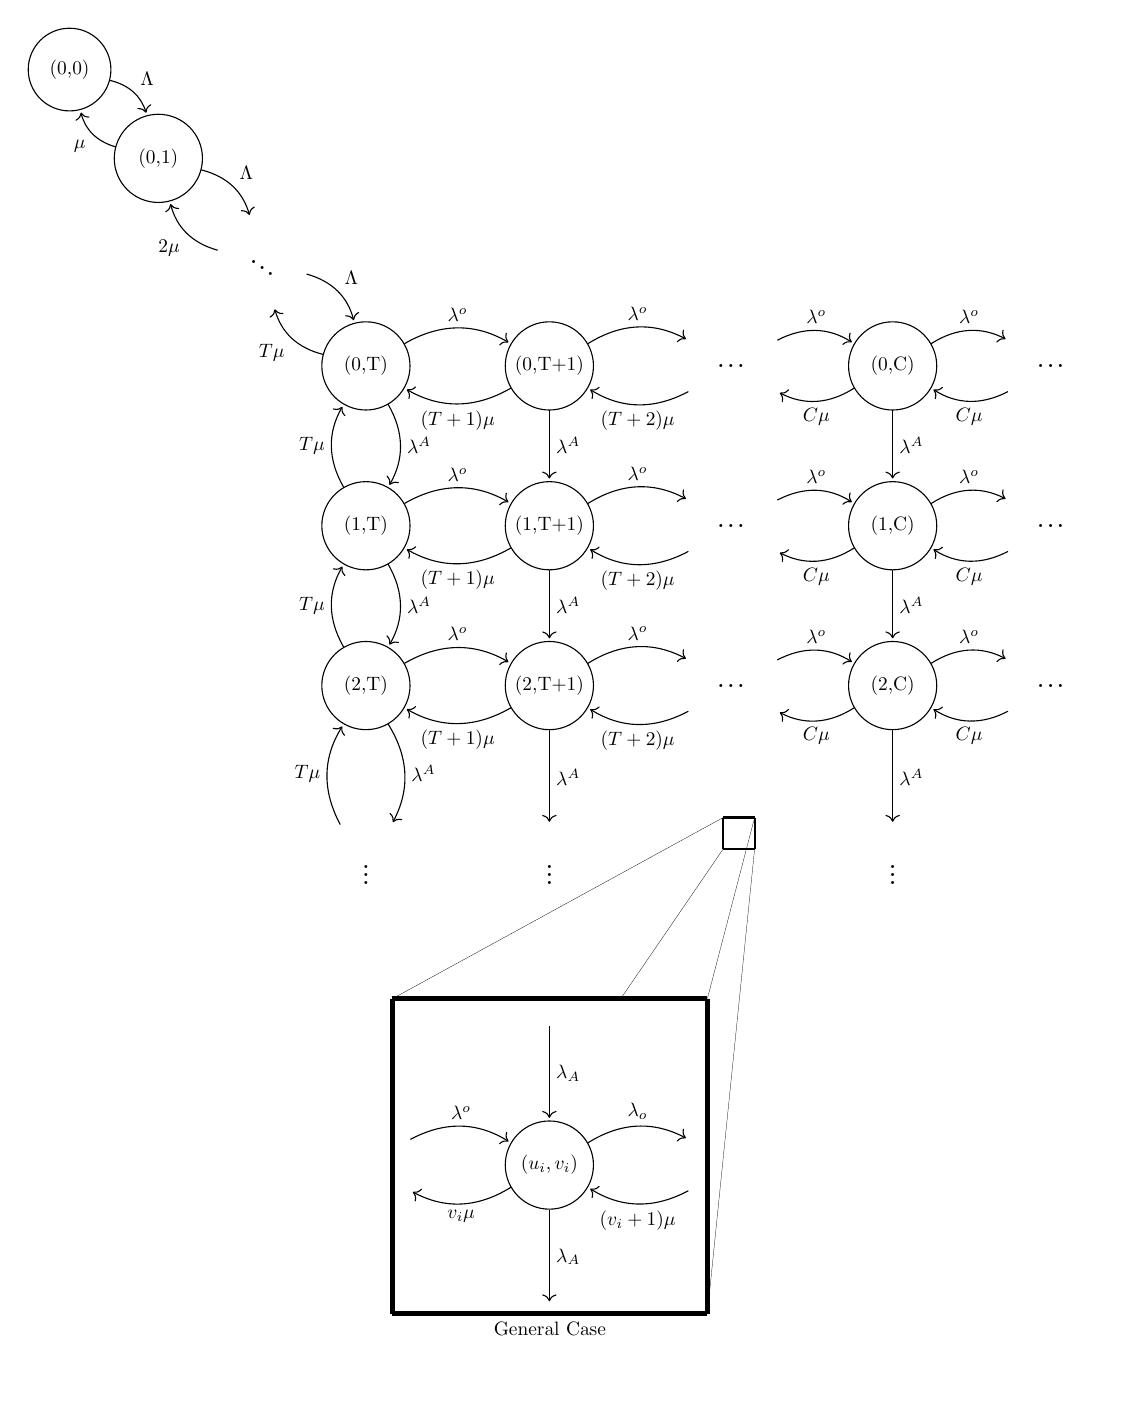
\begin{tikzpicture}[-, node distance = 0.9cm, auto, every node/.style={scale=0.7}]

        % Markov chain variables
        \tikzmath{
            let \initdist = 0.5cm;
            let \altdist = 1.2cm;
            let \minsz = 1.6cm;
        }

        % S_1 and S_2 rectangles
        \tikzmath{
            let \leftOne = -0.8;
            let \rightOne = 2.7;
            let \upOne = 0.8;
            let \downOne = -2.7;
            let \leftTwo = 2.8;
            let \rightTwo = 13;
            let \upTwo = -2.95;
            let \downTwo = -16.4;
        }

        % General case variables
        \tikzmath{
            let \GCsmallx = 8.3;
            let \GCsmally = -9.5;
            let \GCbigx = 4.1;
            let \GCbigy = -11.8;
        }

        % % Rectangle for S1
        % \draw[ultra thin, dashed] (\leftOne, \downOne) -- (\leftOne, \upOne);
        % \draw[ultra thin, dashed] (\leftOne, \upOne) -- (\rightOne, \upOne);
        % \draw[ultra thin, dashed] (\rightOne, \upOne) -- node {\Huge{\( \quad S_1 \)}}(\rightOne, \downOne);
        % \draw[ultra thin, dashed] (\rightOne, \downOne) -- (\leftOne, \downOne);

        % % Rectangle for S2
        % \draw[ultra thin, dashed] (\leftTwo, \downTwo) -- node {\Huge{\( S_2 \quad \)}}(\leftTwo, \upTwo);
        % \draw[ultra thin, dashed] (\leftTwo, \upTwo) -- (\rightTwo, \upTwo);
        % \draw[ultra thin, dashed] (\rightTwo, \upTwo) -- (\rightTwo, \downTwo);
        % \draw[ultra thin, dashed] (\rightTwo, \downTwo) -- (\leftTwo, \downTwo);

        % Small square of general case
        \draw [thick] (\GCsmallx, \GCsmally) -- node {} (\GCsmallx + 0.4, \GCsmally);
        \draw [thick] (\GCsmallx + 0.4, \GCsmally) -- node {} (\GCsmallx + 0.4, \GCsmally - 0.4);
        \draw [thick] (\GCsmallx + 0.4, \GCsmally - 0.4) -- node {} (\GCsmallx, \GCsmally - 0.4);
        \draw [thick] (\GCsmallx, \GCsmally - 0.4) -- node {} (\GCsmallx, \GCsmally);


        % Dashed lines to from small square to big one 
        \draw [ultra thin] (\GCsmallx, \GCsmally) -- node {} (\GCbigx, \GCbigy);
        \draw [ultra thin] (\GCsmallx + 0.4, \GCsmally) -- node {} (\GCbigx + 4, \GCbigy);
        \draw [ultra thin] (\GCsmallx, \GCsmally - 0.4) -- node {} (7, \GCbigy);
        \draw [ultra thin] (\GCsmallx + 0.4, \GCsmally - 0.4) -- node {} (\GCbigx + 4, \GCbigy - 4);
        
        % Big Square of general case
        \draw [ultra thick] (\GCbigx, \GCbigy) -- node {} (\GCbigx + 4, \GCbigy);
        \draw [ultra thick] (\GCbigx + 4, \GCbigy) -- node {} (\GCbigx + 4, \GCbigy - 4);
        \draw [ultra thick] (\GCbigx + 4, \GCbigy - 4) -- node {General Case} (\GCbigx, \GCbigy - 4);
        \draw [ultra thick] (\GCbigx, \GCbigy - 4) -- node {} (\GCbigx, \GCbigy);

        % First Line
        \node[state, minimum size=1.5cm] (zero) {(0,0)};
        \node[state, node distance = \initdist, minimum size=\minsz, below right=of zero] (one) {(0,1)};
        \node[draw=none, node distance = \initdist, minimum size=\minsz, below right=of one] (two) {\textbf{\( \ddots \)}};
        \node[state, node distance = \initdist, minimum size=\minsz, below right=of two] (three) {(0,T)};
        \node[state, node distance = \altdist, minimum size=\minsz, right=of three] (four) {(0,T+1)};
        \node[draw=none, node distance = \altdist, minimum size=\minsz, right=of four] (five) {\textbf{\dots}};
        \node[state, minimum size=\minsz, right=of five] (six) {(0,C)};
        \node[draw=none, minimum size=\minsz, right=of six] (seven) {\textbf{\dots}};

        % Second Line
        \node[state, minimum size=\minsz, below=of three] (three_one) {(1,T)};
        \node[state, minimum size=\minsz, below=of four] (four_one) {(1,T+1)};
        \node[draw=none, minimum size=\minsz, below=of five] (five_one) {\textbf{\dots}};
        \node[state, minimum size=\minsz, right=of five_one] (six_one) {(1,C)};
        \node[draw=none, minimum size=\minsz, right=of six_one] (seven_one) {\textbf{\dots}};
        
        % Third Line
        \node[state, minimum size=\minsz, below=of three_one] (three_two) {(2,T)};
        \node[state, minimum size=\minsz, below=of four_one] (four_two) {(2,T+1)};
        \node[draw=none, minimum size=\minsz, below=of five_one] (five_two) {\textbf{\dots}};
        \node[state, minimum size=\minsz, right=of five_two] (six_two) {(2,C)};
        \node[draw=none, minimum size=\minsz, right=of six_two] (seven_two) {\textbf{\dots}};

        % Fourth line
        \node[draw=none, node distance = \altdist, minimum size=\minsz, below=of three_two] (three_three) {\textbf{\vdots}};
        \node[draw=none, node distance = \altdist, minimum size=\minsz, below=of four_two] (four_three) {\textbf{\vdots}};
        \node[draw=none, node distance = 2cm, minimum size=\minsz, below=of five_two] (five_three) {};
        \node[draw=none, node distance = \altdist, minimum size=\minsz, below=of six_two] (six_three) {\textbf{\vdots}};

        % Fifth line
        % \node[state, node distance = \altdist, minimum size=\minsz, below=of five_three] (general_case_mid) {\( (u_i, v_i) \)};
        \node[draw=none, node distance = 0.3cm, minimum size=\minsz, below=of four_three] (general_case_up) {};
        \node[state, node distance = \altdist, minimum size=\minsz, below=of general_case_up] (general_case_mid) {\( (u_i, v_i) \)};

        \node[draw=none, node distance = \altdist, minimum size=\minsz, below=of general_case_mid] (general_case_down) {};
        \node[draw=none, node distance = \altdist, minimum size=\minsz, left=of general_case_mid] (general_case_left) {};
        \node[draw=none, node distance = \altdist, minimum size=\minsz, right=of general_case_mid] (general_case_right) {};

        \draw[every loop]
            % First Horizontal Edges
            (zero) edge[bend left] node {\( \Lambda \)} (one)
            (one) edge[bend left] node {\( \mu \)} (zero)
            (one) edge[bend left] node {\( \Lambda \)} (two)
            (two) edge[bend left] node {\( 2 \mu \)} (one)
            (two) edge[bend left] node {\( \Lambda \)} (three)
            (three) edge[bend left] node {\( T \mu \)} (two)
            (three) edge[bend left] node {\( \lambda^o \)} (four)
            (four) edge[bend left] node {\( (T+1) \mu \)} (three)
            (four) edge[bend left] node {\( \lambda^o \)} (five)
            (five) edge[bend left] node {\( (T+2) \mu \)} (four)
            (five) edge[bend left] node {\( \lambda^o \)} (six)
            (six) edge[bend left] node {\( C\mu \)} (five)
            (six) edge[bend left] node {\( \lambda^o \)} (seven)
            (seven) edge[bend left] node {\( C\mu \)} (six)

            % Second Horizontal Edges
            (three_one) edge[bend left] node {\( \lambda^o \)} (four_one)
            (four_one) edge[bend left] node {\( (T+1) \mu \)} (three_one)
            (four_one) edge[bend left] node {\( \lambda^o \)} (five_one)
            (five_one) edge[bend left] node {\( (T+2) \mu \)} (four_one)
            (five_one) edge[bend left] node {\( \lambda^o \)} (six_one)
            (six_one) edge[bend left] node {\( C\mu \)} (five_one)
            (six_one) edge[bend left] node {\( \lambda^o \)} (seven_one)
            (seven_one) edge[bend left] node {\( C\mu \)} (six_one)

            % Third Horizontal Edges
            (three_two) edge[bend left] node {\( \lambda^o \)} (four_two)
            (four_two) edge[bend left] node [below] {\( (T+1) \mu \)} (three_two)
            (four_two) edge[bend left] node {\( \lambda^o \)} (five_two)
            (five_two) edge[bend left] node {\( (T+2) \mu \)} (four_two)
            (five_two) edge[bend left] node {\( \lambda^o \)} (six_two)
            (six_two) edge[bend left] node {\( C\mu \)} (five_two)
            (six_two) edge[bend left] node {\( \lambda^o \)} (seven_two)
            (seven_two) edge[bend left] node {\( C\mu \)} (six_two)

            % First Vertical Edges
            (three) edge[bend left] node {\( \lambda^A \)} (three_one)
            (three_one) edge[bend left] node {\( T \mu \)} (three)
            (three_one) edge[bend left] node {\( \lambda^A \)} (three_two)
            (three_two) edge[bend left] node {\( T\mu \)} (three_one)
            (three_two) edge[bend left] node {\( \lambda^A \)} (three_three)
            (three_three) edge[bend left] node {\( T\mu \)} (three_two)

            % Second Vertical Edges
            (four) edge node {\( \lambda^A \)} (four_one)
            (four_one) edge node {\( \lambda^A \)} (four_two)
            (four_two) edge node {\( \lambda^A \)} (four_three)

            % Fourth Vertical Edges
            (six) edge node {\( \lambda^A \)} (six_one)
            (six_one) edge node {\( \lambda^A \)} (six_two)
            (six_two) edge node {\( \lambda^A \)} (six_three)

            % General Case
            (general_case_left) edge[bend left] node {\( \lambda^o \)} (general_case_mid)
            (general_case_mid) edge[bend left] node {\( v_i \mu \)} (general_case_left)
            (general_case_right) edge[bend left] node {\( (v_i +1) \mu \)} (general_case_mid)
            (general_case_mid) edge[bend left] node {\( \lambda_o \)} (general_case_right)
            % (five_three) edge node {\( \lambda_A \)} (general_case_mid)
            (general_case_up) edge node {\( \lambda_A \)} (general_case_mid)
            (general_case_mid) edge node {\( \lambda_A \)} (general_case_down)
            ;
    \end{tikzpicture}
    \caption{Markov chain} 
    \label{Markov_5}
\end{figure}


\newpage
\section{Figures that might be useful}
\begin{figure}[h]
    \centering
    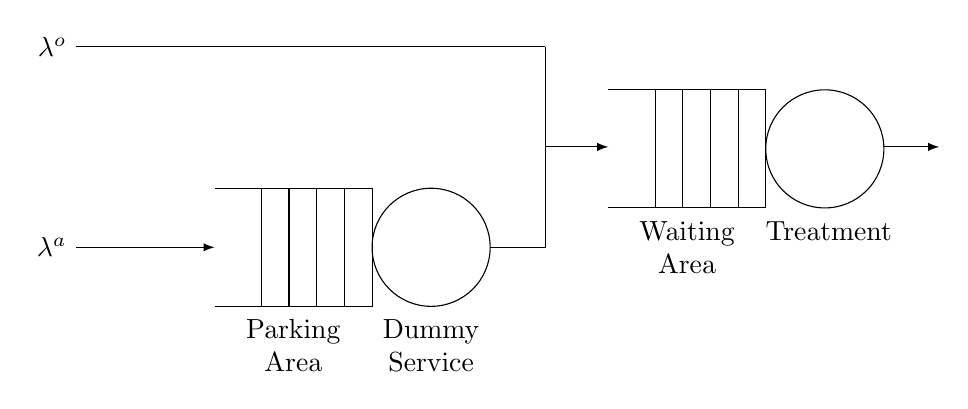
\begin{tikzpicture}[>=latex]
        % the rectangle with vertical rules (Queue 1)
        \draw (0,0) -- ++(2cm,0) -- ++(0,-1.5cm) -- ++(-2cm,0);
        \foreach \i in {1,...,4}
        \draw (2cm-\i*10pt,0) -- +(0,-1.5cm);
        
        % the circle (Queue 1)
        \draw (2.75,-0.75cm) circle [radius=0.75cm];

        % the rectangle with vertical rules (Queue 2)
        \draw (5,1.25) -- ++(2cm,0) -- ++(0,-1.5cm) -- ++(-2cm,0);
        \foreach \i in {1,...,4}
        \draw (7cm-\i*10pt,1.25) -- +(0,-1.5cm);

        % the circle (Queue 2)
        \draw (7.75,0.5) circle [radius=0.75cm];

        % the arrows and labels (Queue 1+2)
        \draw[-] (3.5,-0.75) -- +(20pt,0);
        \draw[<-] (0,-0.75) -- +(-50pt,0) node[left] {\( \lambda^a \)};
        \draw[->] (8.5,0.525) -- +(20pt,0);
        \node[align=center] at (1cm,-2cm) {Parking \\ Area};
        \node[align=center] at (2.75cm,-2cm) {Dummy \\ Service};
        \node[align=center] at (6cm,-0.75cm) {Waiting \\ Area};
        \node[align=center] at (7.8cm,-0.75cm) {Treatment \\ };
        
        \draw (4.2, 1.8) -- +(-169.5pt,0) node[left] {\( \lambda^o \)};
        \draw (4.2, 1.8) -- (4.2, -0.75);
        \draw[->] (4.2, 0.525) -- (5, 0.525);

    \end{tikzpicture}
\end{figure}


\begin{figure}
    \centering
    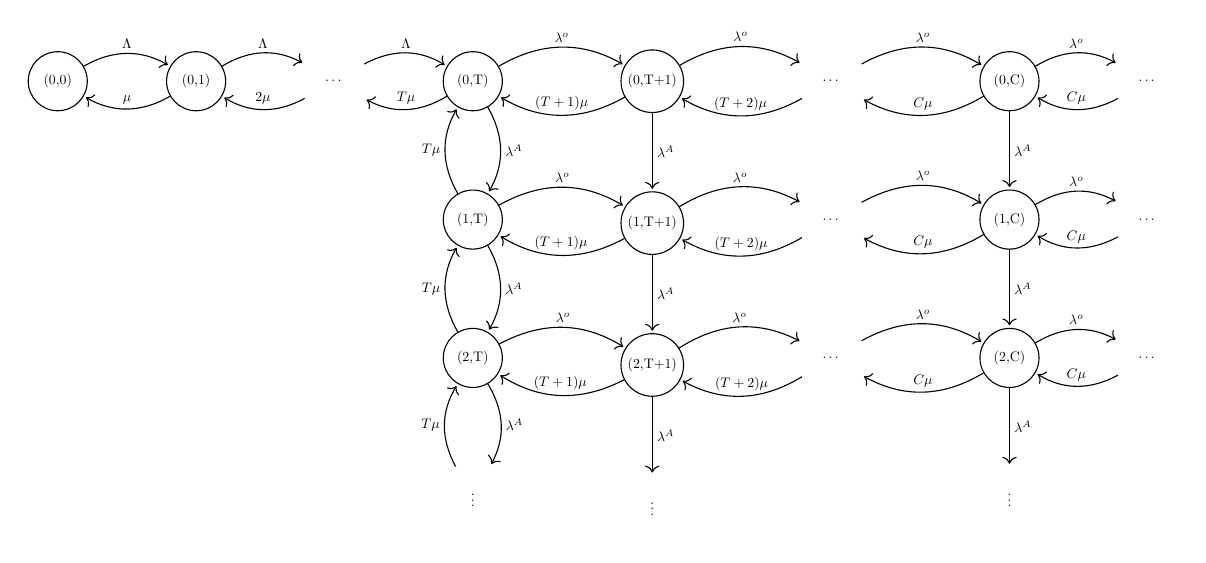
\begin{tikzpicture}[-, node distance = 1cm, auto, every node/.style={scale=0.5}]

        % Variables
        \tikzmath{
            let \altdist = 1.5cm;
            let \minsz = 1.5cm;
        }

        % First Line
        \node[state, minimum size=1.5cm] (zero) {(0,0)};
        \node[state, minimum size=1.5cm,  right=of zero] (one) {(0,1)};
        \node[draw=none, minimum size=1.5cm, right=of one] (two) {\dots};
        \node[state, minimum size=1.5cm, right=of two] (three) {(0,T)};
        \node[state, node distance = \altdist, minimum size=\minsz, right=of three] (four) {(0,T+1)};
        \node[draw=none, node distance = \altdist, minimum size=\minsz, right=of four] (five) {\dots};
        \node[state, node distance = \altdist, minimum size=\minsz, right=of five] (six) {(0,C)};
        \node[draw=none, minimum size=\minsz, right=of six] (seven) {\dots};

        % Second Line
        \node[state, minimum size=\minsz, below=of three] (three_one) {(1,T)};
        \node[state, minimum size=\minsz, below=of four] (four_one) {(1,T+1)};
        \node[draw=none, minimum size=\minsz, below=of five] (five_one) {\dots};
        \node[state, node distance = \altdist, minimum size=\minsz, right=of five_one] (six_one) {(1,C)};
        \node[draw=none, minimum size=\minsz, right=of six_one] (seven_one) {\dots};

        % Third Line
        \node[state, minimum size=\minsz, below=of three_one] (three_two) {(2,T)};
        \node[state, minimum size=\minsz, below=of four_one] (four_two) {(2,T+1)};
        \node[draw=none, minimum size=\minsz, below=of five_one] (five_two) {\dots};
        \node[state, node distance = \altdist, minimum size=\minsz, right=of five_two] (six_two) {(2,C)};
        \node[draw=none, minimum size=\minsz, right=of six_two] (seven_two) {\dots};

        % Fourth line
        \node[draw=none, minimum size=\minsz, below=of three_two] (three_three) {\vdots};
        \node[draw=none, minimum size=\minsz, below=of four_two] (four_three) {\vdots};
        \node[draw=none, minimum size=\minsz, below=of five_two] (five_three) {};
        \node[draw=none, node distance = \altdist, minimum size=\minsz, right=of five_three] (six_three) {\vdots};

        \draw[every loop]
            % First Horizontal Edges
            (zero) edge[bend left] node {\( \Lambda \)} (one)
            (one) edge[bend left] node [above] {\( \mu \)} (zero)
            (one) edge[bend left] node {\( \Lambda \)} (two)
            (two) edge[bend left] node [above] {\( 2 \mu \)} (one)
            (two) edge[bend left] node {\( \Lambda \)} (three)
            (three) edge[bend left] node [above] {\( T \mu \)} (two)
            (three) edge[bend left] node {\( \lambda^o \)} (four)
            (four) edge[bend left] node [above] {\( (T+1) \mu \)} (three)
            (four) edge[bend left] node {\( \lambda^o \)} (five)
            (five) edge[bend left] node [above] {\( (T+2) \mu \)} (four)
            (five) edge[bend left] node {\( \lambda^o \)} (six)
            (six) edge[bend left] node [above] {\( C\mu \)} (five)
            (six) edge[bend left] node {\( \lambda^o \)} (seven)
            (seven) edge[bend left] node [above] {\( C\mu \)} (six)

            % Second Horizontal Edges
            (three_one) edge[bend left] node {\( \lambda^o \)} (four_one)
            (four_one) edge[bend left] node [above] {\( (T+1) \mu \)} (three_one)
            (four_one) edge[bend left] node {\( \lambda^o \)} (five_one)
            (five_one) edge[bend left] node [above] {\( (T+2) \mu \)} (four_one)
            (five_one) edge[bend left] node {\( \lambda^o \)} (six_one)
            (six_one) edge[bend left] node [above] {\( C\mu \)} (five_one)
            (six_one) edge[bend left] node {\( \lambda^o \)} (seven_one)
            (seven_one) edge[bend left] node [above] {\( C\mu \)} (six_one)

            % Third Horizontal Edges
            (three_two) edge[bend left] node {\( \lambda^o \)} (four_two)
            (four_two) edge[bend left] node [above] {\( (T+1) \mu \)} (three_two)
            (four_two) edge[bend left] node {\( \lambda^o \)} (five_two)
            (five_two) edge[bend left] node [above] {\( (T+2) \mu \)} (four_two)
            (five_two) edge[bend left] node {\( \lambda^o \)} (six_two)
            (six_two) edge[bend left] node [above] {\( C\mu \)} (five_two)
            (six_two) edge[bend left] node {\( \lambda^o \)} (seven_two)
            (seven_two) edge[bend left] node [above] {\( C\mu \)} (six_two)

            % First Vertical Edges
            (three) edge[bend left] node {\( \lambda^A \)} (three_one)
            (three_one) edge[bend left] node {\( T \mu \)} (three)
            (three_one) edge[bend left] node {\( \lambda^A \)} (three_two)
            (three_two) edge[bend left] node {\( T\mu \)} (three_one)
            (three_two) edge[bend left] node {\( \lambda^A \)} (three_three)
            (three_three) edge[bend left] node {\( T\mu \)} (three_two)

            % Second Vertical Edges
            (four) edge node {\( \lambda^A \)} (four_one)
            (four_one) edge node {\( \lambda^A \)} (four_two)
            (four_two) edge node {\( \lambda^A \)} (four_three)

            %Third Vertical Edges
            (six) edge node {\( \lambda^A \)} (six_one)
            (six_one) edge node {\( \lambda^A \)} (six_two)
            (six_two) edge node {\( \lambda^A \)} (six_three)
            ;       
    \end{tikzpicture}
    \caption{Markov chains} 
    \label{Markov_2}
\end{figure}



\begin{figure}
    \centering
    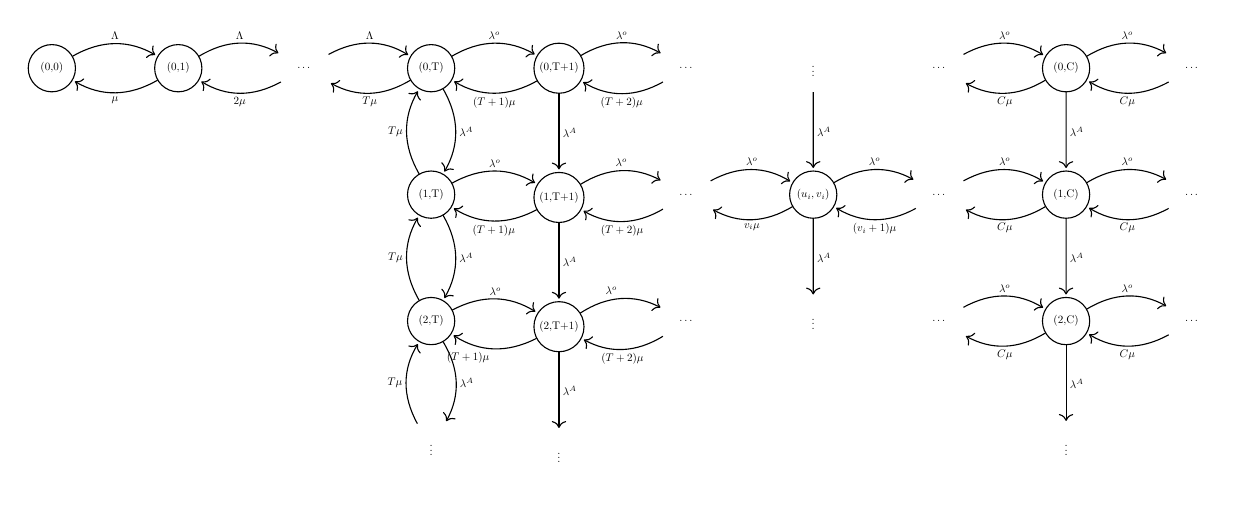
\begin{tikzpicture}[-, node distance = 1cm, auto, every node/.style={scale=0.4}]

        % Variables
        \tikzmath{
            let \altdist = 1cm;
            let \minsz = 1.5cm;
        }

        % First Line
        \node[state, minimum size=1.5cm] (zero) {(0,0)};
        \node[state, minimum size=1.5cm,  right=of zero] (one) {(0,1)};
        \node[draw=none, minimum size=1.5cm, right=of one] (two) {\dots};
        \node[state, minimum size=1.5cm, right=of two] (three) {(0,T)};
        \node[state, node distance = \altdist, minimum size=\minsz, right=of three] (four) {(0,T+1)};
        \node[draw=none, minimum size=\minsz, right=of four] (five) {\dots};
        \node[draw=none, minimum size=\minsz, right=of five] (six) {\vdots};
        \node[draw=none, minimum size=\minsz, right=of six] (seven) {\dots};
        \node[state, minimum size=\minsz, right=of seven] (eight) {(0,C)};
        \node[draw=none, minimum size=\minsz, right=of eight] (nine) {\dots};


        % Second Line
        \node[state, minimum size=\minsz, below=of three] (three_one) {(1,T)};
        \node[state, minimum size=\minsz, below=of four] (four_one) {(1,T+1)};
        \node[draw=none, minimum size=\minsz, below=of five] (five_one) {\dots};
        \node[state, node distance = \altdist, minimum size=\minsz, right=of five_one] (six_one) {\( (u_i, v_i) \)};
        \node[draw=none, minimum size=\minsz, right=of six_one] (seven_one) {\dots};
        \node[state, node distance = \altdist, minimum size=\minsz, right=of seven_one] (eight_one) {(1,C)};
        \node[draw=none, minimum size=\minsz, right=of eight_one] (nine_one) {\dots};
        

        % Third Line
        \node[state, minimum size=\minsz, below=of three_one] (three_two) {(2,T)};
        \node[state, minimum size=\minsz, below=of four_one] (four_two) {(2,T+1)};
        \node[draw=none, minimum size=\minsz, below=of five_one] (five_two) {\dots};
        \node[draw=none, node distance = \altdist, minimum size=\minsz, right=of five_two] (six_two) {\vdots};
        \node[draw=none, minimum size=\minsz, right=of six_two] (seven_two) {\dots};
        \node[state, node distance = \altdist, minimum size=\minsz, right=of seven_two] (eight_two) {(2,C)};
        \node[draw=none, minimum size=\minsz, right=of eight_two] (nine_two) {\dots};

        % Fourth line
        \node[draw=none, minimum size=\minsz, below=of three_two] (three_three) {\vdots};
        \node[draw=none, minimum size=\minsz, below=of four_two] (four_three) {\vdots};
        \node[draw=none, minimum size=\minsz, below=of five_two] (five_three) {};
        \node[draw=none, node distance = \altdist, minimum size=\minsz, right=of five_three] (six_three) {};
        \node[draw=none, node distance = \altdist, minimum size=\minsz, below=of eight_two] (eight_three) {\vdots};


        \draw[every loop]
            % First Horizontal Edges
            (zero) edge[bend left] node {\( \Lambda \)} (one)
            (one) edge[bend left] node {\( \mu \)} (zero)
            (one) edge[bend left] node {\( \Lambda \)} (two)
            (two) edge[bend left] node {\( 2 \mu \)} (one)
            (two) edge[bend left] node {\( \Lambda \)} (three)
            (three) edge[bend left] node {\( T \mu \)} (two)
            (three) edge[bend left] node {\( \lambda^o \)} (four)
            (four) edge[bend left] node {\( (T+1) \mu \)} (three)
            (four) edge[bend left] node {\( \lambda^o \)} (five)
            (five) edge[bend left] node {\( (T+2) \mu \)} (four)
            % (five) edge[bend left] node {\( \lambda^o \)} (six)
            % (six) edge[bend left] node [above] {\( C\mu \)} (five)
            % (six) edge[bend left] node {\( \lambda^o \)} (seven)
            % (seven) edge[bend left] node [above] {\( C\mu \)} (six)
            (seven) edge[bend left] node {\( \lambda^o \)} (eight)
            (eight) edge[bend left] node {\( C\mu \)} (seven)
            (eight) edge[bend left] node {\( \lambda^o \)} (nine)
            (nine) edge[bend left] node {\( C\mu \)} (eight)

            % Second Horizontal Edges
            (three_one) edge[bend left] node {\(\lambda^o\)} (four_one)
            (four_one) edge[bend left] node {\( (T+1) \mu \)} (three_one)
            (four_one) edge[bend left] node {\( \lambda^o \)} (five_one)
            (five_one) edge[bend left] node {\( (T+2) \mu \)} (four_one)
            (five_one) edge[bend left] node {\( \lambda^o \)} (six_one)
            (six_one) edge[bend left] node {\( v_i\mu \)} (five_one)
            (six_one) edge[bend left] node {\( \lambda^o \)} (seven_one)
            (seven_one) edge[bend left] node {\( (v_i+1)\mu \)} (six_one)
            (seven_one) edge[bend left] node {\( \lambda^o \)} (eight_one)
            (eight_one) edge[bend left] node {\( C\mu \)} (seven_one)
            (eight_one) edge[bend left] node {\( \lambda^o \)} (nine_one)
            (nine_one) edge[bend left] node {\( C\mu \)} (eight_one)

            % Third Horizontal Edges
            (three_two) edge[bend left] node {\( \lambda^o \)} (four_two)
            (four_two) edge[bend left] node {\( (T+1) \mu \)} (three_two)
            (four_two) edge[bend left] node {\( \lambda^o \)} (five_two)
            (five_two) edge[bend left] node {\( (T+2) \mu \)} (four_two)
            % (five_two) edge[bend left] node {\( \lambda^o \)} (six_two)
            % (six_two) edge[bend left] node [above] {\( C\mu \)} (five_two)
            % (six_two) edge[bend left] node {\( \lambda^o \)} (seven_two)
            % (seven_two) edge[bend left] node [above] {\( C\mu \)} (six_two)
            (seven_two) edge[bend left] node {\( \lambda^o \)} (eight_two)
            (eight_two) edge[bend left] node {\( C\mu \)} (seven_two)
            (eight_two) edge[bend left] node {\( \lambda^o \)} (nine_two)
            (nine_two) edge[bend left] node {\( C\mu \)} (eight_two)

            % First Vertical Edges
            (three) edge[bend left] node {\( \lambda^A \)} (three_one)
            (three_one) edge[bend left] node {\( T \mu \)} (three)
            (three_one) edge[bend left] node {\( \lambda^A \)} (three_two)
            (three_two) edge[bend left] node {\( T\mu \)} (three_one)
            (three_two) edge[bend left] node {\( \lambda^A \)} (three_three)
            (three_three) edge[bend left] node {\( T\mu \)} (three_two)

            % Second Vertical Edges
            (four) edge node {\( \lambda^A \)} (four_one)
            (four_one) edge node {\( \lambda^A \)} (four_two)
            (four_two) edge node {\( \lambda^A \)} (four_three)

            % Third Vertical Edges
            (six) edge node {\( \lambda^A \)} (six_one)
            (six_one) edge node {\( \lambda^A \)} (six_two)
            % (six_two) edge node {\( \lambda^A \)} (six_three)

            % Fourth Vertical Edges
            (eight) edge node {\( \lambda^A \)} (eight_one)
            (eight_one) edge node {\( \lambda^A \)} (eight_two)
            (eight_two) edge node {\( \lambda^A \)} (eight_three)
            ;       
    \end{tikzpicture}
    \caption{Markov chains} 
    \label{Markov_3}
\end{figure}


\begin{figure}
    \centering
    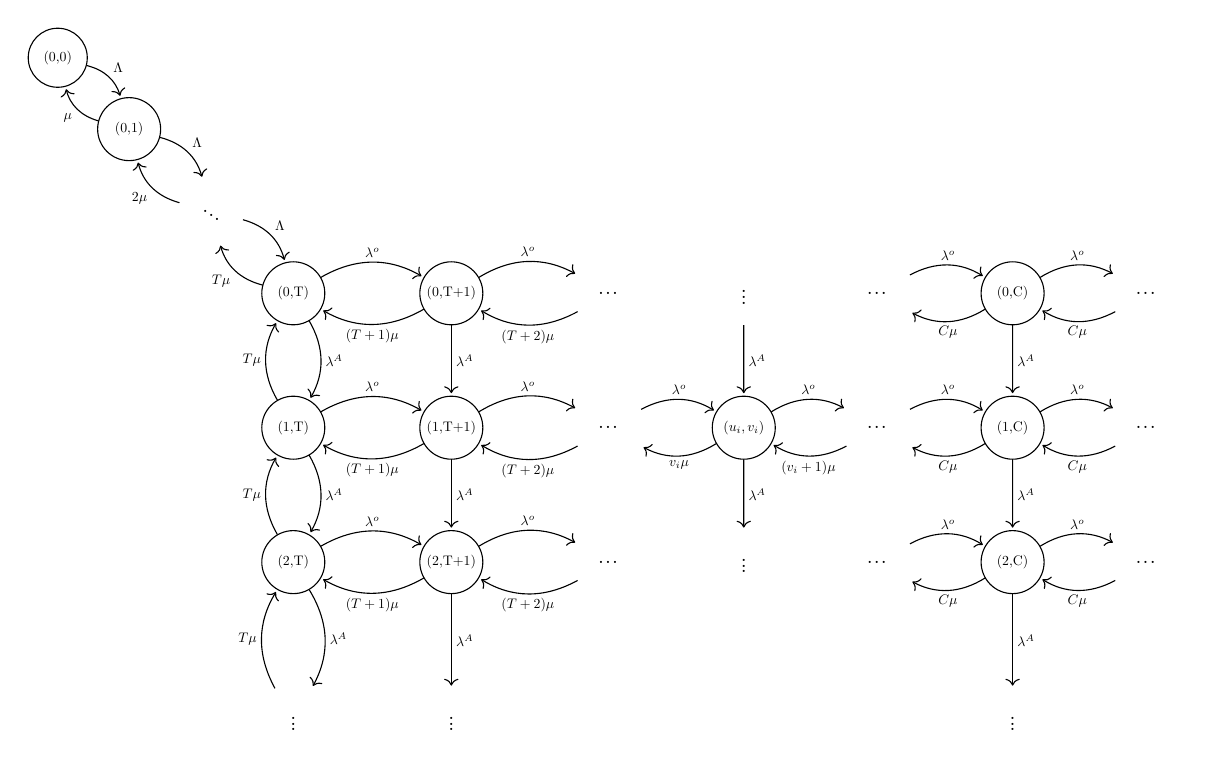
\begin{tikzpicture}[-, node distance = 0.9cm, auto, every node/.style={scale=0.5}]

        % Variables
        \tikzmath{
            let \initdist = 0.5cm;
            let \altdist = 1.2cm;
            let \minsz = 1.6cm;
            let \leftOne = -0.8;
            let \rightOne = 2.2;
            let \upOne = 0.8;
            let \downOne = -2.2;
            let \leftTwo = 2.25;
            let \rightTwo = 14.2;
            let \upTwo = -2.35;
            let \downTwo = -8.8;
        }

        % % Rectangle for S1
        % \draw[ultra thin, dashed] (\leftOne, \downOne) -- (\leftOne, \upOne);
        % \draw[ultra thin, dashed] (\leftOne, \upOne) -- (\rightOne, \upOne);
        % \draw[ultra thin, dashed] (\rightOne, \upOne) -- node {\Huge{\( \quad S_1 \)}}(\rightOne, \downOne);
        % \draw[ultra thin, dashed] (\rightOne, \downOne) -- (\leftOne, \downOne);

        % % Rectangle for S2
        % \draw[ultra thin, dashed] (\leftTwo, \downTwo) -- node {\Huge{\( S_2 \quad \)}}(\leftTwo, \upTwo);
        % \draw[ultra thin, dashed] (\leftTwo, \upTwo) -- (\rightTwo, \upTwo);
        % \draw[ultra thin, dashed] (\rightTwo, \upTwo) -- (\rightTwo, \downTwo);
        % \draw[ultra thin, dashed] (\rightTwo, \downTwo) -- (\leftTwo, \downTwo);

        % First Line
        \node[state, minimum size=1.5cm] (zero) {(0,0)};
        \node[state, node distance = \initdist, minimum size=\minsz, below right=of zero] (one) {(0,1)};
        \node[draw=none, node distance = \initdist, minimum size=\minsz, below right=of one] (two) {\textbf{\( \ddots \)}};
        \node[state, node distance = \initdist, minimum size=\minsz, below right=of two] (three) {(0,T)};
        \node[state, node distance = \altdist, minimum size=\minsz, right=of three] (four) {(0,T+1)};
        \node[draw=none, node distance = \altdist, minimum size=\minsz, right=of four] (five) {\textbf{\dots}};
        \node[draw=none, minimum size=\minsz, right=of five] (six) {\textbf{\vdots}};
        \node[draw=none, minimum size=\minsz, right=of six] (seven) {\textbf{\dots}};
        \node[state, minimum size=\minsz, right=of seven] (eight) {(0,C)};
        \node[draw=none, minimum size=\minsz, right=of eight] (nine) {\textbf{\dots}};


        % Second Line
        \node[state, minimum size=\minsz, below=of three] (three_one) {(1,T)};
        \node[state, minimum size=\minsz, below=of four] (four_one) {(1,T+1)};
        \node[draw=none, minimum size=\minsz, below=of five] (five_one) {\textbf{\dots}};
        \node[state, minimum size=\minsz, right=of five_one] (six_one) {\( (u_i, v_i) \)};
        \node[draw=none, minimum size=\minsz, right=of six_one] (seven_one) {\textbf{\dots}};
        \node[state, minimum size=\minsz, right=of seven_one] (eight_one) {(1,C)};
        \node[draw=none, minimum size=\minsz, right=of eight_one] (nine_one) {\textbf{\dots}};
        

        % Third Line
        \node[state, minimum size=\minsz, below=of three_one] (three_two) {(2,T)};
        \node[state, minimum size=\minsz, below=of four_one] (four_two) {(2,T+1)};
        \node[draw=none, minimum size=\minsz, below=of five_one] (five_two) {\textbf{\dots}};
        \node[draw=none, minimum size=\minsz, right=of five_two] (six_two) {\textbf{\vdots}};
        \node[draw=none, minimum size=\minsz, right=of six_two] (seven_two) {\textbf{\dots}};
        \node[state, minimum size=\minsz, right=of seven_two] (eight_two) {(2,C)};
        \node[draw=none, minimum size=\minsz, right=of eight_two] (nine_two) {\textbf{\dots}};

        % Fourth line
        \node[draw=none, node distance = \altdist, minimum size=\minsz, below=of three_two] (three_three) {\textbf{\vdots}};
        \node[draw=none, node distance = \altdist, minimum size=\minsz, below=of four_two] (four_three) {\textbf{\vdots}};
        \node[draw=none, node distance = \altdist, minimum size=\minsz, below=of five_two] (five_three) {};
        \node[draw=none, node distance = \altdist, minimum size=\minsz, below=of six_two] (six_three) {};
        \node[draw=none, node distance = \altdist, minimum size=\minsz, below=of eight_two] (eight_three) {\textbf{\vdots}};


        \draw[every loop]
            % First Horizontal Edges
            (zero) edge[bend left] node {\( \Lambda \)} (one)
            (one) edge[bend left] node {\( \mu \)} (zero)
            (one) edge[bend left] node {\( \Lambda \)} (two)
            (two) edge[bend left] node {\( 2 \mu \)} (one)
            (two) edge[bend left] node {\( \Lambda \)} (three)
            (three) edge[bend left] node {\( T \mu \)} (two)
            (three) edge[bend left] node {\( \lambda^o \)} (four)
            (four) edge[bend left] node {\( (T+1) \mu \)} (three)
            (four) edge[bend left] node {\( \lambda^o \)} (five)
            (five) edge[bend left] node {\( (T+2) \mu \)} (four)
            % (five) edge[bend left] node {\( \lambda^o \)} (six)
            % (six) edge[bend left] node [above] {\( C\mu \)} (five)
            % (six) edge[bend left] node {\( \lambda^o \)} (seven)
            % (seven) edge[bend left] node [above] {\( C\mu \)} (six)
            (seven) edge[bend left] node {\( \lambda^o \)} (eight)
            (eight) edge[bend left] node {\( C\mu \)} (seven)
            (eight) edge[bend left] node {\( \lambda^o \)} (nine)
            (nine) edge[bend left] node {\( C\mu \)} (eight)

            % Second Horizontal Edges
            (three_one) edge[bend left] node {\( \lambda^o \)} (four_one)
            (four_one) edge[bend left] node {\( (T+1) \mu \)} (three_one)
            (four_one) edge[bend left] node {\( \lambda^o \)} (five_one)
            (five_one) edge[bend left] node {\( (T+2) \mu \)} (four_one)
            (five_one) edge[bend left] node {\( \lambda^o \)} (six_one)
            (six_one) edge[bend left] node {\( v_i\mu \)} (five_one)
            (six_one) edge[bend left] node {\( \lambda^o \)} (seven_one)
            (seven_one) edge[bend left] node {\( (v_i+1)\mu \)} (six_one)
            (seven_one) edge[bend left] node {\( \lambda^o \)} (eight_one)
            (eight_one) edge[bend left] node {\( C\mu \)} (seven_one)
            (eight_one) edge[bend left] node {\( \lambda^o \)} (nine_one)
            (nine_one) edge[bend left] node {\( C\mu \)} (eight_one)

            % Third Horizontal Edges
            (three_two) edge[bend left] node {\( \lambda^o \)} (four_two)
            (four_two) edge[bend left] node [below] {\( (T+1) \mu \)} (three_two)
            (four_two) edge[bend left] node {\( \lambda^o \)} (five_two)
            (five_two) edge[bend left] node {\( (T+2) \mu \)} (four_two)
            % (five_two) edge[bend left] node {\( \lambda^o \)} (six_two)
            % (six_two) edge[bend left] node [above] {\( C\mu \)} (five_two)
            % (six_two) edge[bend left] node {\( \lambda^o \)} (seven_two)
            % (seven_two) edge[bend left] node [above] {\( C\mu \)} (six_two)
            (seven_two) edge[bend left] node {\( \lambda^o \)} (eight_two)
            (eight_two) edge[bend left] node {\( C\mu \)} (seven_two)
            (eight_two) edge[bend left] node {\( \lambda^o \)} (nine_two)
            (nine_two) edge[bend left] node {\( C\mu \)} (eight_two)

            % First Vertical Edges
            (three) edge[bend left] node {\( \lambda^A \)} (three_one)
            (three_one) edge[bend left] node {\( T \mu \)} (three)
            (three_one) edge[bend left] node {\( \lambda^A \)} (three_two)
            (three_two) edge[bend left] node {\( T\mu \)} (three_one)
            (three_two) edge[bend left] node {\( \lambda^A \)} (three_three)
            (three_three) edge[bend left] node {\( T\mu \)} (three_two)

            % Second Vertical Edges
            (four) edge node {\( \lambda^A \)} (four_one)
            (four_one) edge node {\( \lambda^A \)} (four_two)
            (four_two) edge node {\( \lambda^A \)} (four_three)

            % Third Vertical Edges
            (six) edge node {\( \lambda^A \)} (six_one)
            (six_one) edge node {\( \lambda^A \)} (six_two)
            % (six_two) edge node {\( \lambda^A \)} (six_three)

            % Fourth Vertical Edges
            (eight) edge node {\( \lambda^A \)} (eight_one)
            (eight_one) edge node {\( \lambda^A \)} (eight_two)
            (eight_two) edge node {\( \lambda^A \)} (eight_three)
            ;       
    \end{tikzpicture}
    \caption{Markov chains} 
    \label{Markov_4}
\end{figure}




\begin{figure}
    \centering
    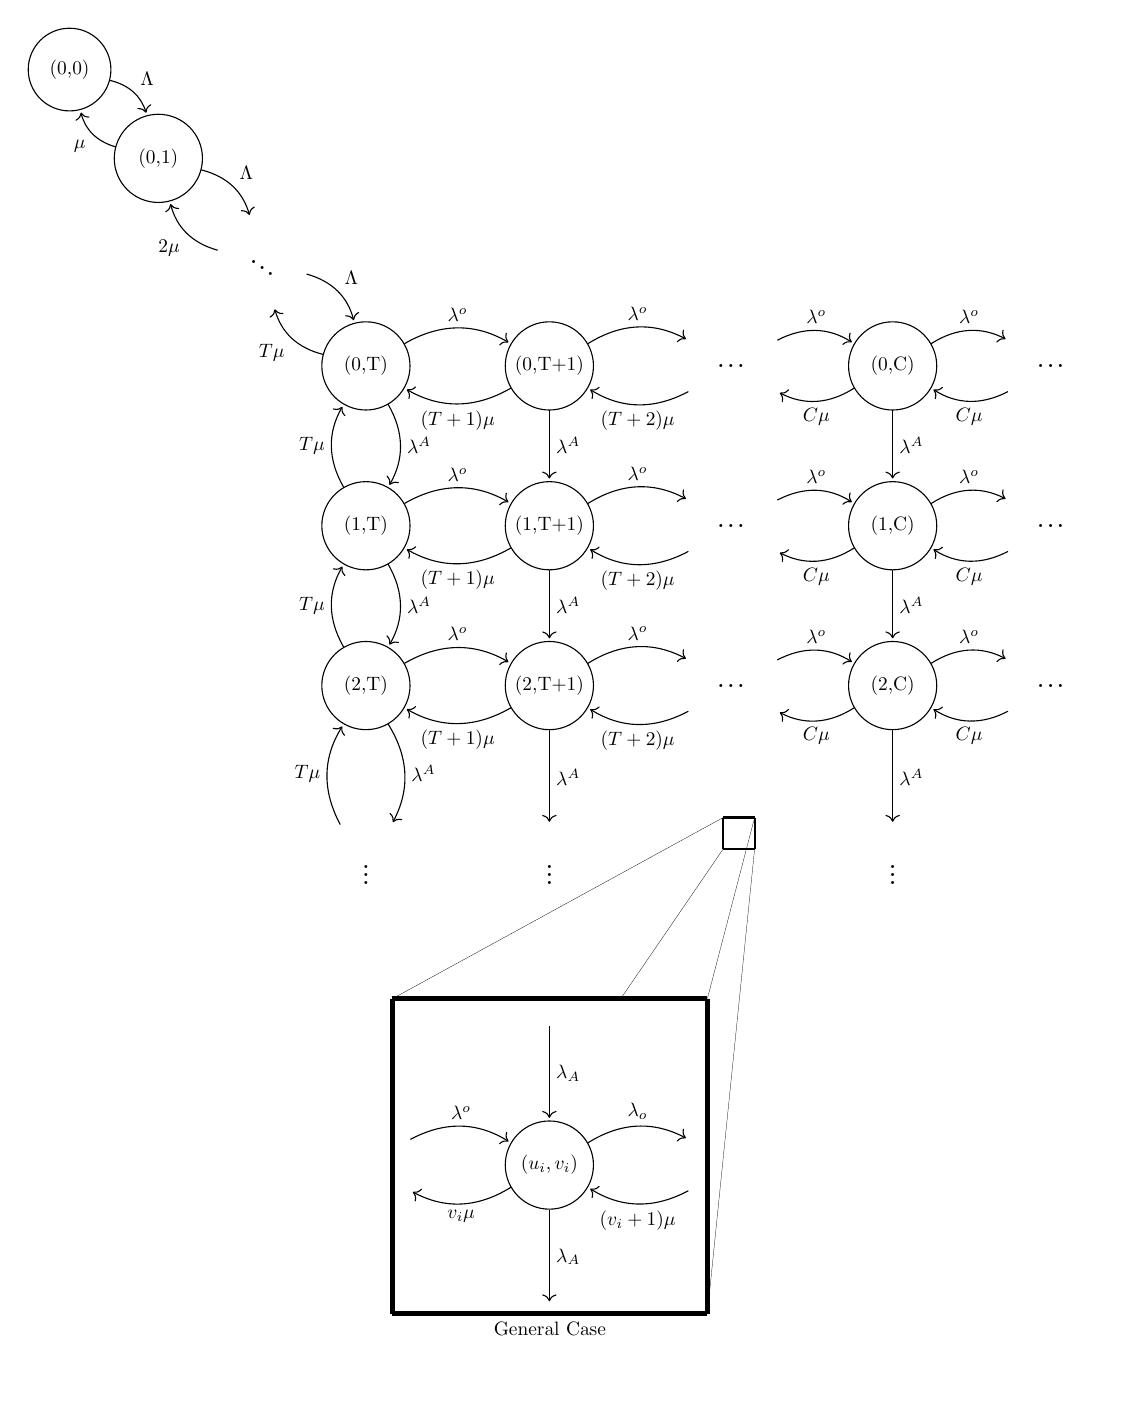
\begin{tikzpicture}[-, node distance = 0.9cm, auto, every node/.style={scale=0.7}]

        % Markov chain variables
        \tikzmath{
            let \initdist = 0.5cm;
            let \altdist = 1.2cm;
            let \minsz = 1.6cm;
        }

        % S_1 and S_2 rectangles
        \tikzmath{
            let \leftOne = -0.8;
            let \rightOne = 2.7;
            let \upOne = 0.8;
            let \downOne = -2.7;
            let \leftTwo = 2.8;
            let \rightTwo = 13;
            let \upTwo = -2.95;
            let \downTwo = -16.4;
        }

        % General case variables
        \tikzmath{
            let \GCsmallx = 8.3;
            let \GCsmally = -9.5;
            let \GCbigx = 4.1;
            let \GCbigy = -11.8;
        }

        % % Rectangle for S1
        % \draw[ultra thin, dashed] (\leftOne, \downOne) -- (\leftOne, \upOne);
        % \draw[ultra thin, dashed] (\leftOne, \upOne) -- (\rightOne, \upOne);
        % \draw[ultra thin, dashed] (\rightOne, \upOne) -- node {\Huge{\( \quad S_1 \)}}(\rightOne, \downOne);
        % \draw[ultra thin, dashed] (\rightOne, \downOne) -- (\leftOne, \downOne);

        % % Rectangle for S2
        % \draw[ultra thin, dashed] (\leftTwo, \downTwo) -- node {\Huge{\( S_2 \quad \)}}(\leftTwo, \upTwo);
        % \draw[ultra thin, dashed] (\leftTwo, \upTwo) -- (\rightTwo, \upTwo);
        % \draw[ultra thin, dashed] (\rightTwo, \upTwo) -- (\rightTwo, \downTwo);
        % \draw[ultra thin, dashed] (\rightTwo, \downTwo) -- (\leftTwo, \downTwo);

        % Small square of general case
        \draw [thick] (\GCsmallx, \GCsmally) -- node {} (\GCsmallx + 0.4, \GCsmally);
        \draw [thick] (\GCsmallx + 0.4, \GCsmally) -- node {} (\GCsmallx + 0.4, \GCsmally - 0.4);
        \draw [thick] (\GCsmallx + 0.4, \GCsmally - 0.4) -- node {} (\GCsmallx, \GCsmally - 0.4);
        \draw [thick] (\GCsmallx, \GCsmally - 0.4) -- node {} (\GCsmallx, \GCsmally);


        % Dashed lines to from small square to big one 
        \draw [ultra thin] (\GCsmallx, \GCsmally) -- node {} (\GCbigx, \GCbigy);
        \draw [ultra thin] (\GCsmallx + 0.4, \GCsmally) -- node {} (\GCbigx + 4, \GCbigy);
        \draw [ultra thin] (\GCsmallx, \GCsmally - 0.4) -- node {} (7, \GCbigy);
        \draw [ultra thin] (\GCsmallx + 0.4, \GCsmally - 0.4) -- node {} (\GCbigx + 4, \GCbigy - 4);
        
        % Big Square of general case
        \draw [ultra thick] (\GCbigx, \GCbigy) -- node {} (\GCbigx + 4, \GCbigy);
        \draw [ultra thick] (\GCbigx + 4, \GCbigy) -- node {} (\GCbigx + 4, \GCbigy - 4);
        \draw [ultra thick] (\GCbigx + 4, \GCbigy - 4) -- node {General Case} (\GCbigx, \GCbigy - 4);
        \draw [ultra thick] (\GCbigx, \GCbigy - 4) -- node {} (\GCbigx, \GCbigy);

        % First Line
        \node[state, minimum size=1.5cm] (zero) {(0,0)};
        \node[state, node distance = \initdist, minimum size=\minsz, below right=of zero] (one) {(0,1)};
        \node[draw=none, node distance = \initdist, minimum size=\minsz, below right=of one] (two) {\textbf{\( \ddots \)}};
        \node[state, node distance = \initdist, minimum size=\minsz, below right=of two] (three) {(0,T)};
        \node[state, node distance = \altdist, minimum size=\minsz, right=of three] (four) {(0,T+1)};
        \node[draw=none, node distance = \altdist, minimum size=\minsz, right=of four] (five) {\textbf{\dots}};
        \node[state, minimum size=\minsz, right=of five] (six) {(0,C)};
        \node[draw=none, minimum size=\minsz, right=of six] (seven) {\textbf{\dots}};

        % Second Line
        \node[state, minimum size=\minsz, below=of three] (three_one) {(1,T)};
        \node[state, minimum size=\minsz, below=of four] (four_one) {(1,T+1)};
        \node[draw=none, minimum size=\minsz, below=of five] (five_one) {\textbf{\dots}};
        \node[state, minimum size=\minsz, right=of five_one] (six_one) {(1,C)};
        \node[draw=none, minimum size=\minsz, right=of six_one] (seven_one) {\textbf{\dots}};
        
        % Third Line
        \node[state, minimum size=\minsz, below=of three_one] (three_two) {(2,T)};
        \node[state, minimum size=\minsz, below=of four_one] (four_two) {(2,T+1)};
        \node[draw=none, minimum size=\minsz, below=of five_one] (five_two) {\textbf{\dots}};
        \node[state, minimum size=\minsz, right=of five_two] (six_two) {(2,C)};
        \node[draw=none, minimum size=\minsz, right=of six_two] (seven_two) {\textbf{\dots}};

        % Fourth line
        \node[draw=none, node distance = \altdist, minimum size=\minsz, below=of three_two] (three_three) {\textbf{\vdots}};
        \node[draw=none, node distance = \altdist, minimum size=\minsz, below=of four_two] (four_three) {\textbf{\vdots}};
        \node[draw=none, node distance = 2cm, minimum size=\minsz, below=of five_two] (five_three) {};
        \node[draw=none, node distance = \altdist, minimum size=\minsz, below=of six_two] (six_three) {\textbf{\vdots}};

        % Fifth line
        % \node[state, node distance = \altdist, minimum size=\minsz, below=of five_three] (general_case_mid) {\( (u_i, v_i) \)};
        \node[draw=none, node distance = 0.3cm, minimum size=\minsz, below=of four_three] (general_case_up) {};
        \node[state, node distance = \altdist, minimum size=\minsz, below=of general_case_up] (general_case_mid) {\( (u_i, v_i) \)};

        \node[draw=none, node distance = \altdist, minimum size=\minsz, below=of general_case_mid] (general_case_down) {};
        \node[draw=none, node distance = \altdist, minimum size=\minsz, left=of general_case_mid] (general_case_left) {};
        \node[draw=none, node distance = \altdist, minimum size=\minsz, right=of general_case_mid] (general_case_right) {};

        \draw[every loop]
            % First Horizontal Edges
            (zero) edge[bend left] node {\( \Lambda \)} (one)
            (one) edge[bend left] node {\( \mu \)} (zero)
            (one) edge[bend left] node {\( \Lambda \)} (two)
            (two) edge[bend left] node {\( 2 \mu \)} (one)
            (two) edge[bend left] node {\( \Lambda \)} (three)
            (three) edge[bend left] node {\( T \mu \)} (two)
            (three) edge[bend left] node {\( \lambda^o \)} (four)
            (four) edge[bend left] node {\( (T+1) \mu \)} (three)
            (four) edge[bend left] node {\( \lambda^o \)} (five)
            (five) edge[bend left] node {\( (T+2) \mu \)} (four)
            (five) edge[bend left] node {\( \lambda^o \)} (six)
            (six) edge[bend left] node {\( C\mu \)} (five)
            (six) edge[bend left] node {\( \lambda^o \)} (seven)
            (seven) edge[bend left] node {\( C\mu \)} (six)

            % Second Horizontal Edges
            (three_one) edge[bend left] node {\( \lambda^o \)} (four_one)
            (four_one) edge[bend left] node {\( (T+1) \mu \)} (three_one)
            (four_one) edge[bend left] node {\( \lambda^o \)} (five_one)
            (five_one) edge[bend left] node {\( (T+2) \mu \)} (four_one)
            (five_one) edge[bend left] node {\( \lambda^o \)} (six_one)
            (six_one) edge[bend left] node {\( C\mu \)} (five_one)
            (six_one) edge[bend left] node {\( \lambda^o \)} (seven_one)
            (seven_one) edge[bend left] node {\( C\mu \)} (six_one)

            % Third Horizontal Edges
            (three_two) edge[bend left] node {\( \lambda^o \)} (four_two)
            (four_two) edge[bend left] node [below] {\( (T+1) \mu \)} (three_two)
            (four_two) edge[bend left] node {\( \lambda^o \)} (five_two)
            (five_two) edge[bend left] node {\( (T+2) \mu \)} (four_two)
            (five_two) edge[bend left] node {\( \lambda^o \)} (six_two)
            (six_two) edge[bend left] node {\( C\mu \)} (five_two)
            (six_two) edge[bend left] node {\( \lambda^o \)} (seven_two)
            (seven_two) edge[bend left] node {\( C\mu \)} (six_two)

            % First Vertical Edges
            (three) edge[bend left] node {\( \lambda^A \)} (three_one)
            (three_one) edge[bend left] node {\( T \mu \)} (three)
            (three_one) edge[bend left] node {\( \lambda^A \)} (three_two)
            (three_two) edge[bend left] node {\( T\mu \)} (three_one)
            (three_two) edge[bend left] node {\( \lambda^A \)} (three_three)
            (three_three) edge[bend left] node {\( T\mu \)} (three_two)

            % Second Vertical Edges
            (four) edge node {\( \lambda^A \)} (four_one)
            (four_one) edge node {\( \lambda^A \)} (four_two)
            (four_two) edge node {\( \lambda^A \)} (four_three)

            % Fourth Vertical Edges
            (six) edge node {\( \lambda^A \)} (six_one)
            (six_one) edge node {\( \lambda^A \)} (six_two)
            (six_two) edge node {\( \lambda^A \)} (six_three)

            % General Case
            (general_case_left) edge[bend left] node {\( \lambda^o \)} (general_case_mid)
            (general_case_mid) edge[bend left] node {\( v_i \mu \)} (general_case_left)
            (general_case_right) edge[bend left] node {\( (v_i +1) \mu \)} (general_case_mid)
            (general_case_mid) edge[bend left] node {\( \lambda_o \)} (general_case_right)
            % (five_three) edge node {\( \lambda_A \)} (general_case_mid)
            (general_case_up) edge node {\( \lambda_A \)} (general_case_mid)
            (general_case_mid) edge node {\( \lambda_A \)} (general_case_down)
            ;
    \end{tikzpicture}
    \caption{Markov chain} 
    \label{Markov_5}
\end{figure}



\newpage
% Heatmap comparisons
\section{Figures that might be useful}
\begin{figure}[h]
    \centering
    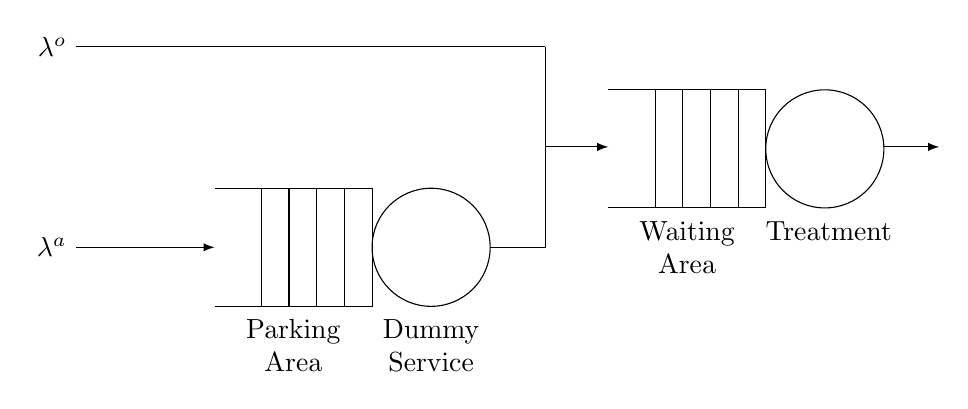
\begin{tikzpicture}[>=latex]
        % the rectangle with vertical rules (Queue 1)
        \draw (0,0) -- ++(2cm,0) -- ++(0,-1.5cm) -- ++(-2cm,0);
        \foreach \i in {1,...,4}
        \draw (2cm-\i*10pt,0) -- +(0,-1.5cm);
        
        % the circle (Queue 1)
        \draw (2.75,-0.75cm) circle [radius=0.75cm];

        % the rectangle with vertical rules (Queue 2)
        \draw (5,1.25) -- ++(2cm,0) -- ++(0,-1.5cm) -- ++(-2cm,0);
        \foreach \i in {1,...,4}
        \draw (7cm-\i*10pt,1.25) -- +(0,-1.5cm);

        % the circle (Queue 2)
        \draw (7.75,0.5) circle [radius=0.75cm];

        % the arrows and labels (Queue 1+2)
        \draw[-] (3.5,-0.75) -- +(20pt,0);
        \draw[<-] (0,-0.75) -- +(-50pt,0) node[left] {\( \lambda^a \)};
        \draw[->] (8.5,0.525) -- +(20pt,0);
        \node[align=center] at (1cm,-2cm) {Parking \\ Area};
        \node[align=center] at (2.75cm,-2cm) {Dummy \\ Service};
        \node[align=center] at (6cm,-0.75cm) {Waiting \\ Area};
        \node[align=center] at (7.8cm,-0.75cm) {Treatment \\ };
        
        \draw (4.2, 1.8) -- +(-169.5pt,0) node[left] {\( \lambda^o \)};
        \draw (4.2, 1.8) -- (4.2, -0.75);
        \draw[->] (4.2, 0.525) -- (5, 0.525);

    \end{tikzpicture}
\end{figure}


\begin{figure}
    \centering
    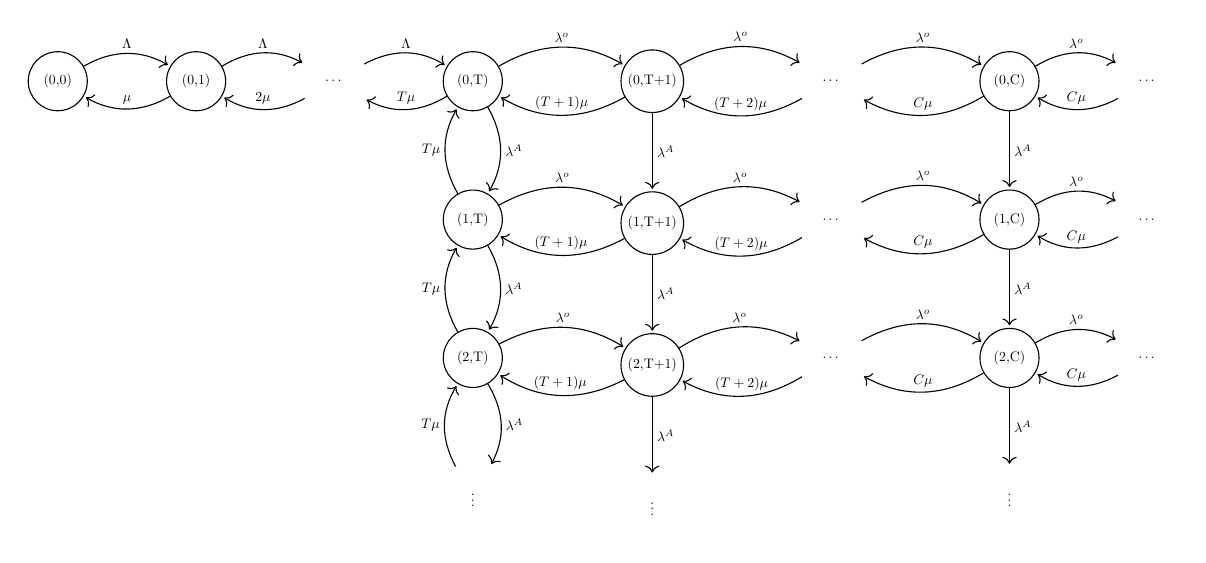
\begin{tikzpicture}[-, node distance = 1cm, auto, every node/.style={scale=0.5}]

        % Variables
        \tikzmath{
            let \altdist = 1.5cm;
            let \minsz = 1.5cm;
        }

        % First Line
        \node[state, minimum size=1.5cm] (zero) {(0,0)};
        \node[state, minimum size=1.5cm,  right=of zero] (one) {(0,1)};
        \node[draw=none, minimum size=1.5cm, right=of one] (two) {\dots};
        \node[state, minimum size=1.5cm, right=of two] (three) {(0,T)};
        \node[state, node distance = \altdist, minimum size=\minsz, right=of three] (four) {(0,T+1)};
        \node[draw=none, node distance = \altdist, minimum size=\minsz, right=of four] (five) {\dots};
        \node[state, node distance = \altdist, minimum size=\minsz, right=of five] (six) {(0,C)};
        \node[draw=none, minimum size=\minsz, right=of six] (seven) {\dots};

        % Second Line
        \node[state, minimum size=\minsz, below=of three] (three_one) {(1,T)};
        \node[state, minimum size=\minsz, below=of four] (four_one) {(1,T+1)};
        \node[draw=none, minimum size=\minsz, below=of five] (five_one) {\dots};
        \node[state, node distance = \altdist, minimum size=\minsz, right=of five_one] (six_one) {(1,C)};
        \node[draw=none, minimum size=\minsz, right=of six_one] (seven_one) {\dots};

        % Third Line
        \node[state, minimum size=\minsz, below=of three_one] (three_two) {(2,T)};
        \node[state, minimum size=\minsz, below=of four_one] (four_two) {(2,T+1)};
        \node[draw=none, minimum size=\minsz, below=of five_one] (five_two) {\dots};
        \node[state, node distance = \altdist, minimum size=\minsz, right=of five_two] (six_two) {(2,C)};
        \node[draw=none, minimum size=\minsz, right=of six_two] (seven_two) {\dots};

        % Fourth line
        \node[draw=none, minimum size=\minsz, below=of three_two] (three_three) {\vdots};
        \node[draw=none, minimum size=\minsz, below=of four_two] (four_three) {\vdots};
        \node[draw=none, minimum size=\minsz, below=of five_two] (five_three) {};
        \node[draw=none, node distance = \altdist, minimum size=\minsz, right=of five_three] (six_three) {\vdots};

        \draw[every loop]
            % First Horizontal Edges
            (zero) edge[bend left] node {\( \Lambda \)} (one)
            (one) edge[bend left] node [above] {\( \mu \)} (zero)
            (one) edge[bend left] node {\( \Lambda \)} (two)
            (two) edge[bend left] node [above] {\( 2 \mu \)} (one)
            (two) edge[bend left] node {\( \Lambda \)} (three)
            (three) edge[bend left] node [above] {\( T \mu \)} (two)
            (three) edge[bend left] node {\( \lambda^o \)} (four)
            (four) edge[bend left] node [above] {\( (T+1) \mu \)} (three)
            (four) edge[bend left] node {\( \lambda^o \)} (five)
            (five) edge[bend left] node [above] {\( (T+2) \mu \)} (four)
            (five) edge[bend left] node {\( \lambda^o \)} (six)
            (six) edge[bend left] node [above] {\( C\mu \)} (five)
            (six) edge[bend left] node {\( \lambda^o \)} (seven)
            (seven) edge[bend left] node [above] {\( C\mu \)} (six)

            % Second Horizontal Edges
            (three_one) edge[bend left] node {\( \lambda^o \)} (four_one)
            (four_one) edge[bend left] node [above] {\( (T+1) \mu \)} (three_one)
            (four_one) edge[bend left] node {\( \lambda^o \)} (five_one)
            (five_one) edge[bend left] node [above] {\( (T+2) \mu \)} (four_one)
            (five_one) edge[bend left] node {\( \lambda^o \)} (six_one)
            (six_one) edge[bend left] node [above] {\( C\mu \)} (five_one)
            (six_one) edge[bend left] node {\( \lambda^o \)} (seven_one)
            (seven_one) edge[bend left] node [above] {\( C\mu \)} (six_one)

            % Third Horizontal Edges
            (three_two) edge[bend left] node {\( \lambda^o \)} (four_two)
            (four_two) edge[bend left] node [above] {\( (T+1) \mu \)} (three_two)
            (four_two) edge[bend left] node {\( \lambda^o \)} (five_two)
            (five_two) edge[bend left] node [above] {\( (T+2) \mu \)} (four_two)
            (five_two) edge[bend left] node {\( \lambda^o \)} (six_two)
            (six_two) edge[bend left] node [above] {\( C\mu \)} (five_two)
            (six_two) edge[bend left] node {\( \lambda^o \)} (seven_two)
            (seven_two) edge[bend left] node [above] {\( C\mu \)} (six_two)

            % First Vertical Edges
            (three) edge[bend left] node {\( \lambda^A \)} (three_one)
            (three_one) edge[bend left] node {\( T \mu \)} (three)
            (three_one) edge[bend left] node {\( \lambda^A \)} (three_two)
            (three_two) edge[bend left] node {\( T\mu \)} (three_one)
            (three_two) edge[bend left] node {\( \lambda^A \)} (three_three)
            (three_three) edge[bend left] node {\( T\mu \)} (three_two)

            % Second Vertical Edges
            (four) edge node {\( \lambda^A \)} (four_one)
            (four_one) edge node {\( \lambda^A \)} (four_two)
            (four_two) edge node {\( \lambda^A \)} (four_three)

            %Third Vertical Edges
            (six) edge node {\( \lambda^A \)} (six_one)
            (six_one) edge node {\( \lambda^A \)} (six_two)
            (six_two) edge node {\( \lambda^A \)} (six_three)
            ;       
    \end{tikzpicture}
    \caption{Markov chains} 
    \label{Markov_2}
\end{figure}



\begin{figure}
    \centering
    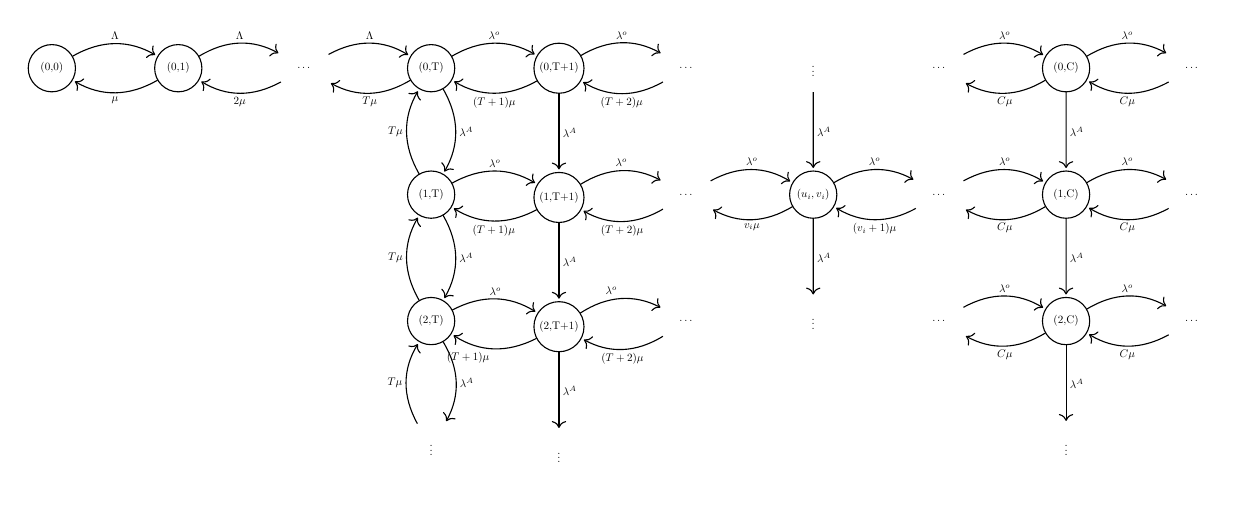
\begin{tikzpicture}[-, node distance = 1cm, auto, every node/.style={scale=0.4}]

        % Variables
        \tikzmath{
            let \altdist = 1cm;
            let \minsz = 1.5cm;
        }

        % First Line
        \node[state, minimum size=1.5cm] (zero) {(0,0)};
        \node[state, minimum size=1.5cm,  right=of zero] (one) {(0,1)};
        \node[draw=none, minimum size=1.5cm, right=of one] (two) {\dots};
        \node[state, minimum size=1.5cm, right=of two] (three) {(0,T)};
        \node[state, node distance = \altdist, minimum size=\minsz, right=of three] (four) {(0,T+1)};
        \node[draw=none, minimum size=\minsz, right=of four] (five) {\dots};
        \node[draw=none, minimum size=\minsz, right=of five] (six) {\vdots};
        \node[draw=none, minimum size=\minsz, right=of six] (seven) {\dots};
        \node[state, minimum size=\minsz, right=of seven] (eight) {(0,C)};
        \node[draw=none, minimum size=\minsz, right=of eight] (nine) {\dots};


        % Second Line
        \node[state, minimum size=\minsz, below=of three] (three_one) {(1,T)};
        \node[state, minimum size=\minsz, below=of four] (four_one) {(1,T+1)};
        \node[draw=none, minimum size=\minsz, below=of five] (five_one) {\dots};
        \node[state, node distance = \altdist, minimum size=\minsz, right=of five_one] (six_one) {\( (u_i, v_i) \)};
        \node[draw=none, minimum size=\minsz, right=of six_one] (seven_one) {\dots};
        \node[state, node distance = \altdist, minimum size=\minsz, right=of seven_one] (eight_one) {(1,C)};
        \node[draw=none, minimum size=\minsz, right=of eight_one] (nine_one) {\dots};
        

        % Third Line
        \node[state, minimum size=\minsz, below=of three_one] (three_two) {(2,T)};
        \node[state, minimum size=\minsz, below=of four_one] (four_two) {(2,T+1)};
        \node[draw=none, minimum size=\minsz, below=of five_one] (five_two) {\dots};
        \node[draw=none, node distance = \altdist, minimum size=\minsz, right=of five_two] (six_two) {\vdots};
        \node[draw=none, minimum size=\minsz, right=of six_two] (seven_two) {\dots};
        \node[state, node distance = \altdist, minimum size=\minsz, right=of seven_two] (eight_two) {(2,C)};
        \node[draw=none, minimum size=\minsz, right=of eight_two] (nine_two) {\dots};

        % Fourth line
        \node[draw=none, minimum size=\minsz, below=of three_two] (three_three) {\vdots};
        \node[draw=none, minimum size=\minsz, below=of four_two] (four_three) {\vdots};
        \node[draw=none, minimum size=\minsz, below=of five_two] (five_three) {};
        \node[draw=none, node distance = \altdist, minimum size=\minsz, right=of five_three] (six_three) {};
        \node[draw=none, node distance = \altdist, minimum size=\minsz, below=of eight_two] (eight_three) {\vdots};


        \draw[every loop]
            % First Horizontal Edges
            (zero) edge[bend left] node {\( \Lambda \)} (one)
            (one) edge[bend left] node {\( \mu \)} (zero)
            (one) edge[bend left] node {\( \Lambda \)} (two)
            (two) edge[bend left] node {\( 2 \mu \)} (one)
            (two) edge[bend left] node {\( \Lambda \)} (three)
            (three) edge[bend left] node {\( T \mu \)} (two)
            (three) edge[bend left] node {\( \lambda^o \)} (four)
            (four) edge[bend left] node {\( (T+1) \mu \)} (three)
            (four) edge[bend left] node {\( \lambda^o \)} (five)
            (five) edge[bend left] node {\( (T+2) \mu \)} (four)
            % (five) edge[bend left] node {\( \lambda^o \)} (six)
            % (six) edge[bend left] node [above] {\( C\mu \)} (five)
            % (six) edge[bend left] node {\( \lambda^o \)} (seven)
            % (seven) edge[bend left] node [above] {\( C\mu \)} (six)
            (seven) edge[bend left] node {\( \lambda^o \)} (eight)
            (eight) edge[bend left] node {\( C\mu \)} (seven)
            (eight) edge[bend left] node {\( \lambda^o \)} (nine)
            (nine) edge[bend left] node {\( C\mu \)} (eight)

            % Second Horizontal Edges
            (three_one) edge[bend left] node {\(\lambda^o\)} (four_one)
            (four_one) edge[bend left] node {\( (T+1) \mu \)} (three_one)
            (four_one) edge[bend left] node {\( \lambda^o \)} (five_one)
            (five_one) edge[bend left] node {\( (T+2) \mu \)} (four_one)
            (five_one) edge[bend left] node {\( \lambda^o \)} (six_one)
            (six_one) edge[bend left] node {\( v_i\mu \)} (five_one)
            (six_one) edge[bend left] node {\( \lambda^o \)} (seven_one)
            (seven_one) edge[bend left] node {\( (v_i+1)\mu \)} (six_one)
            (seven_one) edge[bend left] node {\( \lambda^o \)} (eight_one)
            (eight_one) edge[bend left] node {\( C\mu \)} (seven_one)
            (eight_one) edge[bend left] node {\( \lambda^o \)} (nine_one)
            (nine_one) edge[bend left] node {\( C\mu \)} (eight_one)

            % Third Horizontal Edges
            (three_two) edge[bend left] node {\( \lambda^o \)} (four_two)
            (four_two) edge[bend left] node {\( (T+1) \mu \)} (three_two)
            (four_two) edge[bend left] node {\( \lambda^o \)} (five_two)
            (five_two) edge[bend left] node {\( (T+2) \mu \)} (four_two)
            % (five_two) edge[bend left] node {\( \lambda^o \)} (six_two)
            % (six_two) edge[bend left] node [above] {\( C\mu \)} (five_two)
            % (six_two) edge[bend left] node {\( \lambda^o \)} (seven_two)
            % (seven_two) edge[bend left] node [above] {\( C\mu \)} (six_two)
            (seven_two) edge[bend left] node {\( \lambda^o \)} (eight_two)
            (eight_two) edge[bend left] node {\( C\mu \)} (seven_two)
            (eight_two) edge[bend left] node {\( \lambda^o \)} (nine_two)
            (nine_two) edge[bend left] node {\( C\mu \)} (eight_two)

            % First Vertical Edges
            (three) edge[bend left] node {\( \lambda^A \)} (three_one)
            (three_one) edge[bend left] node {\( T \mu \)} (three)
            (three_one) edge[bend left] node {\( \lambda^A \)} (three_two)
            (three_two) edge[bend left] node {\( T\mu \)} (three_one)
            (three_two) edge[bend left] node {\( \lambda^A \)} (three_three)
            (three_three) edge[bend left] node {\( T\mu \)} (three_two)

            % Second Vertical Edges
            (four) edge node {\( \lambda^A \)} (four_one)
            (four_one) edge node {\( \lambda^A \)} (four_two)
            (four_two) edge node {\( \lambda^A \)} (four_three)

            % Third Vertical Edges
            (six) edge node {\( \lambda^A \)} (six_one)
            (six_one) edge node {\( \lambda^A \)} (six_two)
            % (six_two) edge node {\( \lambda^A \)} (six_three)

            % Fourth Vertical Edges
            (eight) edge node {\( \lambda^A \)} (eight_one)
            (eight_one) edge node {\( \lambda^A \)} (eight_two)
            (eight_two) edge node {\( \lambda^A \)} (eight_three)
            ;       
    \end{tikzpicture}
    \caption{Markov chains} 
    \label{Markov_3}
\end{figure}


\begin{figure}
    \centering
    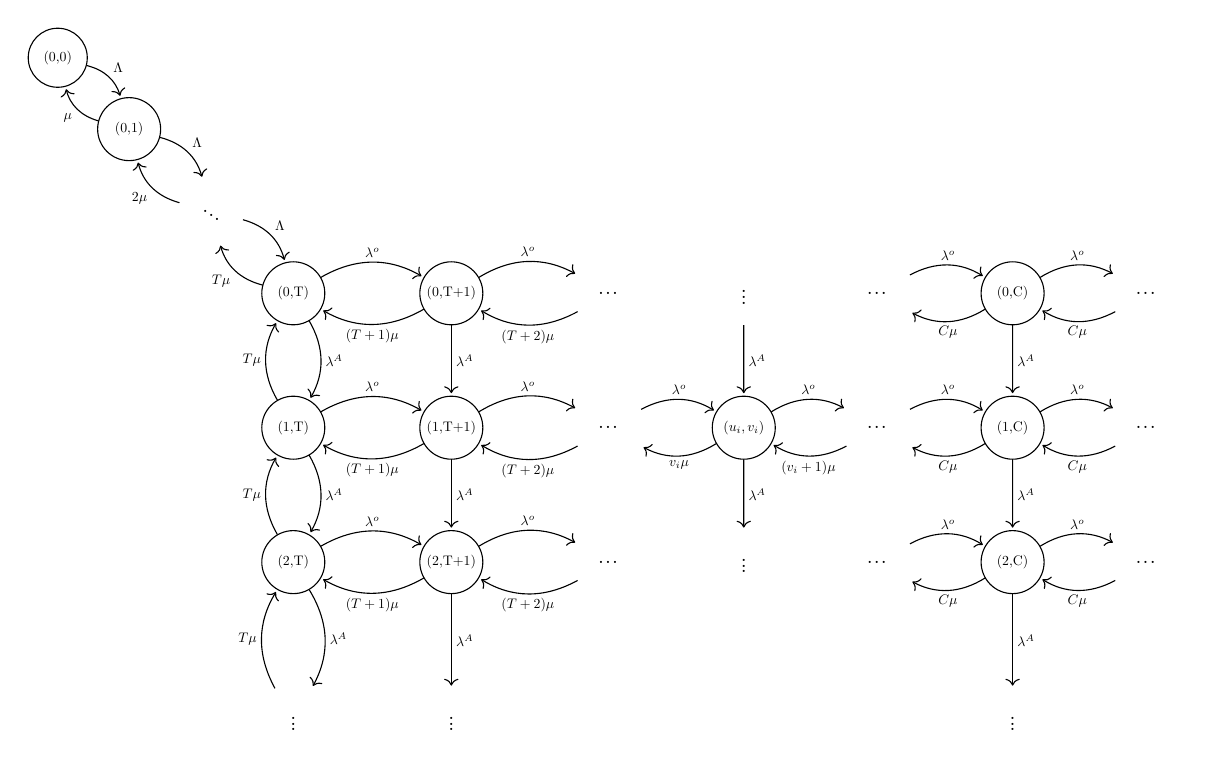
\begin{tikzpicture}[-, node distance = 0.9cm, auto, every node/.style={scale=0.5}]

        % Variables
        \tikzmath{
            let \initdist = 0.5cm;
            let \altdist = 1.2cm;
            let \minsz = 1.6cm;
            let \leftOne = -0.8;
            let \rightOne = 2.2;
            let \upOne = 0.8;
            let \downOne = -2.2;
            let \leftTwo = 2.25;
            let \rightTwo = 14.2;
            let \upTwo = -2.35;
            let \downTwo = -8.8;
        }

        % % Rectangle for S1
        % \draw[ultra thin, dashed] (\leftOne, \downOne) -- (\leftOne, \upOne);
        % \draw[ultra thin, dashed] (\leftOne, \upOne) -- (\rightOne, \upOne);
        % \draw[ultra thin, dashed] (\rightOne, \upOne) -- node {\Huge{\( \quad S_1 \)}}(\rightOne, \downOne);
        % \draw[ultra thin, dashed] (\rightOne, \downOne) -- (\leftOne, \downOne);

        % % Rectangle for S2
        % \draw[ultra thin, dashed] (\leftTwo, \downTwo) -- node {\Huge{\( S_2 \quad \)}}(\leftTwo, \upTwo);
        % \draw[ultra thin, dashed] (\leftTwo, \upTwo) -- (\rightTwo, \upTwo);
        % \draw[ultra thin, dashed] (\rightTwo, \upTwo) -- (\rightTwo, \downTwo);
        % \draw[ultra thin, dashed] (\rightTwo, \downTwo) -- (\leftTwo, \downTwo);

        % First Line
        \node[state, minimum size=1.5cm] (zero) {(0,0)};
        \node[state, node distance = \initdist, minimum size=\minsz, below right=of zero] (one) {(0,1)};
        \node[draw=none, node distance = \initdist, minimum size=\minsz, below right=of one] (two) {\textbf{\( \ddots \)}};
        \node[state, node distance = \initdist, minimum size=\minsz, below right=of two] (three) {(0,T)};
        \node[state, node distance = \altdist, minimum size=\minsz, right=of three] (four) {(0,T+1)};
        \node[draw=none, node distance = \altdist, minimum size=\minsz, right=of four] (five) {\textbf{\dots}};
        \node[draw=none, minimum size=\minsz, right=of five] (six) {\textbf{\vdots}};
        \node[draw=none, minimum size=\minsz, right=of six] (seven) {\textbf{\dots}};
        \node[state, minimum size=\minsz, right=of seven] (eight) {(0,C)};
        \node[draw=none, minimum size=\minsz, right=of eight] (nine) {\textbf{\dots}};


        % Second Line
        \node[state, minimum size=\minsz, below=of three] (three_one) {(1,T)};
        \node[state, minimum size=\minsz, below=of four] (four_one) {(1,T+1)};
        \node[draw=none, minimum size=\minsz, below=of five] (five_one) {\textbf{\dots}};
        \node[state, minimum size=\minsz, right=of five_one] (six_one) {\( (u_i, v_i) \)};
        \node[draw=none, minimum size=\minsz, right=of six_one] (seven_one) {\textbf{\dots}};
        \node[state, minimum size=\minsz, right=of seven_one] (eight_one) {(1,C)};
        \node[draw=none, minimum size=\minsz, right=of eight_one] (nine_one) {\textbf{\dots}};
        

        % Third Line
        \node[state, minimum size=\minsz, below=of three_one] (three_two) {(2,T)};
        \node[state, minimum size=\minsz, below=of four_one] (four_two) {(2,T+1)};
        \node[draw=none, minimum size=\minsz, below=of five_one] (five_two) {\textbf{\dots}};
        \node[draw=none, minimum size=\minsz, right=of five_two] (six_two) {\textbf{\vdots}};
        \node[draw=none, minimum size=\minsz, right=of six_two] (seven_two) {\textbf{\dots}};
        \node[state, minimum size=\minsz, right=of seven_two] (eight_two) {(2,C)};
        \node[draw=none, minimum size=\minsz, right=of eight_two] (nine_two) {\textbf{\dots}};

        % Fourth line
        \node[draw=none, node distance = \altdist, minimum size=\minsz, below=of three_two] (three_three) {\textbf{\vdots}};
        \node[draw=none, node distance = \altdist, minimum size=\minsz, below=of four_two] (four_three) {\textbf{\vdots}};
        \node[draw=none, node distance = \altdist, minimum size=\minsz, below=of five_two] (five_three) {};
        \node[draw=none, node distance = \altdist, minimum size=\minsz, below=of six_two] (six_three) {};
        \node[draw=none, node distance = \altdist, minimum size=\minsz, below=of eight_two] (eight_three) {\textbf{\vdots}};


        \draw[every loop]
            % First Horizontal Edges
            (zero) edge[bend left] node {\( \Lambda \)} (one)
            (one) edge[bend left] node {\( \mu \)} (zero)
            (one) edge[bend left] node {\( \Lambda \)} (two)
            (two) edge[bend left] node {\( 2 \mu \)} (one)
            (two) edge[bend left] node {\( \Lambda \)} (three)
            (three) edge[bend left] node {\( T \mu \)} (two)
            (three) edge[bend left] node {\( \lambda^o \)} (four)
            (four) edge[bend left] node {\( (T+1) \mu \)} (three)
            (four) edge[bend left] node {\( \lambda^o \)} (five)
            (five) edge[bend left] node {\( (T+2) \mu \)} (four)
            % (five) edge[bend left] node {\( \lambda^o \)} (six)
            % (six) edge[bend left] node [above] {\( C\mu \)} (five)
            % (six) edge[bend left] node {\( \lambda^o \)} (seven)
            % (seven) edge[bend left] node [above] {\( C\mu \)} (six)
            (seven) edge[bend left] node {\( \lambda^o \)} (eight)
            (eight) edge[bend left] node {\( C\mu \)} (seven)
            (eight) edge[bend left] node {\( \lambda^o \)} (nine)
            (nine) edge[bend left] node {\( C\mu \)} (eight)

            % Second Horizontal Edges
            (three_one) edge[bend left] node {\( \lambda^o \)} (four_one)
            (four_one) edge[bend left] node {\( (T+1) \mu \)} (three_one)
            (four_one) edge[bend left] node {\( \lambda^o \)} (five_one)
            (five_one) edge[bend left] node {\( (T+2) \mu \)} (four_one)
            (five_one) edge[bend left] node {\( \lambda^o \)} (six_one)
            (six_one) edge[bend left] node {\( v_i\mu \)} (five_one)
            (six_one) edge[bend left] node {\( \lambda^o \)} (seven_one)
            (seven_one) edge[bend left] node {\( (v_i+1)\mu \)} (six_one)
            (seven_one) edge[bend left] node {\( \lambda^o \)} (eight_one)
            (eight_one) edge[bend left] node {\( C\mu \)} (seven_one)
            (eight_one) edge[bend left] node {\( \lambda^o \)} (nine_one)
            (nine_one) edge[bend left] node {\( C\mu \)} (eight_one)

            % Third Horizontal Edges
            (three_two) edge[bend left] node {\( \lambda^o \)} (four_two)
            (four_two) edge[bend left] node [below] {\( (T+1) \mu \)} (three_two)
            (four_two) edge[bend left] node {\( \lambda^o \)} (five_two)
            (five_two) edge[bend left] node {\( (T+2) \mu \)} (four_two)
            % (five_two) edge[bend left] node {\( \lambda^o \)} (six_two)
            % (six_two) edge[bend left] node [above] {\( C\mu \)} (five_two)
            % (six_two) edge[bend left] node {\( \lambda^o \)} (seven_two)
            % (seven_two) edge[bend left] node [above] {\( C\mu \)} (six_two)
            (seven_two) edge[bend left] node {\( \lambda^o \)} (eight_two)
            (eight_two) edge[bend left] node {\( C\mu \)} (seven_two)
            (eight_two) edge[bend left] node {\( \lambda^o \)} (nine_two)
            (nine_two) edge[bend left] node {\( C\mu \)} (eight_two)

            % First Vertical Edges
            (three) edge[bend left] node {\( \lambda^A \)} (three_one)
            (three_one) edge[bend left] node {\( T \mu \)} (three)
            (three_one) edge[bend left] node {\( \lambda^A \)} (three_two)
            (three_two) edge[bend left] node {\( T\mu \)} (three_one)
            (three_two) edge[bend left] node {\( \lambda^A \)} (three_three)
            (three_three) edge[bend left] node {\( T\mu \)} (three_two)

            % Second Vertical Edges
            (four) edge node {\( \lambda^A \)} (four_one)
            (four_one) edge node {\( \lambda^A \)} (four_two)
            (four_two) edge node {\( \lambda^A \)} (four_three)

            % Third Vertical Edges
            (six) edge node {\( \lambda^A \)} (six_one)
            (six_one) edge node {\( \lambda^A \)} (six_two)
            % (six_two) edge node {\( \lambda^A \)} (six_three)

            % Fourth Vertical Edges
            (eight) edge node {\( \lambda^A \)} (eight_one)
            (eight_one) edge node {\( \lambda^A \)} (eight_two)
            (eight_two) edge node {\( \lambda^A \)} (eight_three)
            ;       
    \end{tikzpicture}
    \caption{Markov chains} 
    \label{Markov_4}
\end{figure}




\begin{figure}
    \centering
    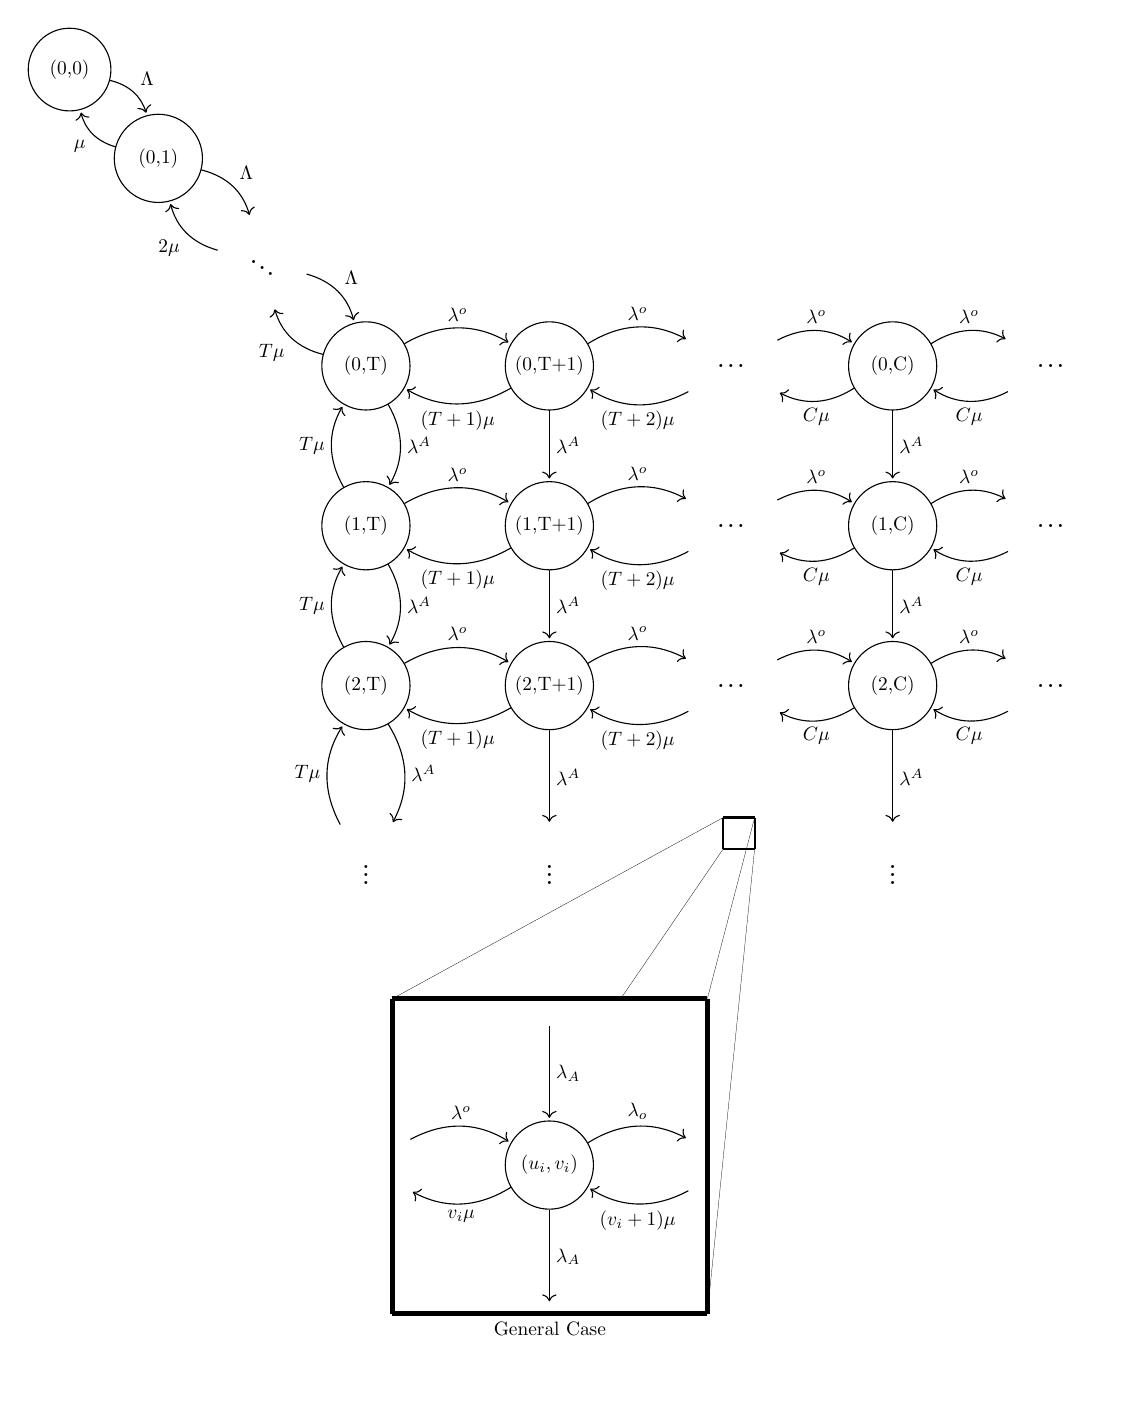
\begin{tikzpicture}[-, node distance = 0.9cm, auto, every node/.style={scale=0.7}]

        % Markov chain variables
        \tikzmath{
            let \initdist = 0.5cm;
            let \altdist = 1.2cm;
            let \minsz = 1.6cm;
        }

        % S_1 and S_2 rectangles
        \tikzmath{
            let \leftOne = -0.8;
            let \rightOne = 2.7;
            let \upOne = 0.8;
            let \downOne = -2.7;
            let \leftTwo = 2.8;
            let \rightTwo = 13;
            let \upTwo = -2.95;
            let \downTwo = -16.4;
        }

        % General case variables
        \tikzmath{
            let \GCsmallx = 8.3;
            let \GCsmally = -9.5;
            let \GCbigx = 4.1;
            let \GCbigy = -11.8;
        }

        % % Rectangle for S1
        % \draw[ultra thin, dashed] (\leftOne, \downOne) -- (\leftOne, \upOne);
        % \draw[ultra thin, dashed] (\leftOne, \upOne) -- (\rightOne, \upOne);
        % \draw[ultra thin, dashed] (\rightOne, \upOne) -- node {\Huge{\( \quad S_1 \)}}(\rightOne, \downOne);
        % \draw[ultra thin, dashed] (\rightOne, \downOne) -- (\leftOne, \downOne);

        % % Rectangle for S2
        % \draw[ultra thin, dashed] (\leftTwo, \downTwo) -- node {\Huge{\( S_2 \quad \)}}(\leftTwo, \upTwo);
        % \draw[ultra thin, dashed] (\leftTwo, \upTwo) -- (\rightTwo, \upTwo);
        % \draw[ultra thin, dashed] (\rightTwo, \upTwo) -- (\rightTwo, \downTwo);
        % \draw[ultra thin, dashed] (\rightTwo, \downTwo) -- (\leftTwo, \downTwo);

        % Small square of general case
        \draw [thick] (\GCsmallx, \GCsmally) -- node {} (\GCsmallx + 0.4, \GCsmally);
        \draw [thick] (\GCsmallx + 0.4, \GCsmally) -- node {} (\GCsmallx + 0.4, \GCsmally - 0.4);
        \draw [thick] (\GCsmallx + 0.4, \GCsmally - 0.4) -- node {} (\GCsmallx, \GCsmally - 0.4);
        \draw [thick] (\GCsmallx, \GCsmally - 0.4) -- node {} (\GCsmallx, \GCsmally);


        % Dashed lines to from small square to big one 
        \draw [ultra thin] (\GCsmallx, \GCsmally) -- node {} (\GCbigx, \GCbigy);
        \draw [ultra thin] (\GCsmallx + 0.4, \GCsmally) -- node {} (\GCbigx + 4, \GCbigy);
        \draw [ultra thin] (\GCsmallx, \GCsmally - 0.4) -- node {} (7, \GCbigy);
        \draw [ultra thin] (\GCsmallx + 0.4, \GCsmally - 0.4) -- node {} (\GCbigx + 4, \GCbigy - 4);
        
        % Big Square of general case
        \draw [ultra thick] (\GCbigx, \GCbigy) -- node {} (\GCbigx + 4, \GCbigy);
        \draw [ultra thick] (\GCbigx + 4, \GCbigy) -- node {} (\GCbigx + 4, \GCbigy - 4);
        \draw [ultra thick] (\GCbigx + 4, \GCbigy - 4) -- node {General Case} (\GCbigx, \GCbigy - 4);
        \draw [ultra thick] (\GCbigx, \GCbigy - 4) -- node {} (\GCbigx, \GCbigy);

        % First Line
        \node[state, minimum size=1.5cm] (zero) {(0,0)};
        \node[state, node distance = \initdist, minimum size=\minsz, below right=of zero] (one) {(0,1)};
        \node[draw=none, node distance = \initdist, minimum size=\minsz, below right=of one] (two) {\textbf{\( \ddots \)}};
        \node[state, node distance = \initdist, minimum size=\minsz, below right=of two] (three) {(0,T)};
        \node[state, node distance = \altdist, minimum size=\minsz, right=of three] (four) {(0,T+1)};
        \node[draw=none, node distance = \altdist, minimum size=\minsz, right=of four] (five) {\textbf{\dots}};
        \node[state, minimum size=\minsz, right=of five] (six) {(0,C)};
        \node[draw=none, minimum size=\minsz, right=of six] (seven) {\textbf{\dots}};

        % Second Line
        \node[state, minimum size=\minsz, below=of three] (three_one) {(1,T)};
        \node[state, minimum size=\minsz, below=of four] (four_one) {(1,T+1)};
        \node[draw=none, minimum size=\minsz, below=of five] (five_one) {\textbf{\dots}};
        \node[state, minimum size=\minsz, right=of five_one] (six_one) {(1,C)};
        \node[draw=none, minimum size=\minsz, right=of six_one] (seven_one) {\textbf{\dots}};
        
        % Third Line
        \node[state, minimum size=\minsz, below=of three_one] (three_two) {(2,T)};
        \node[state, minimum size=\minsz, below=of four_one] (four_two) {(2,T+1)};
        \node[draw=none, minimum size=\minsz, below=of five_one] (five_two) {\textbf{\dots}};
        \node[state, minimum size=\minsz, right=of five_two] (six_two) {(2,C)};
        \node[draw=none, minimum size=\minsz, right=of six_two] (seven_two) {\textbf{\dots}};

        % Fourth line
        \node[draw=none, node distance = \altdist, minimum size=\minsz, below=of three_two] (three_three) {\textbf{\vdots}};
        \node[draw=none, node distance = \altdist, minimum size=\minsz, below=of four_two] (four_three) {\textbf{\vdots}};
        \node[draw=none, node distance = 2cm, minimum size=\minsz, below=of five_two] (five_three) {};
        \node[draw=none, node distance = \altdist, minimum size=\minsz, below=of six_two] (six_three) {\textbf{\vdots}};

        % Fifth line
        % \node[state, node distance = \altdist, minimum size=\minsz, below=of five_three] (general_case_mid) {\( (u_i, v_i) \)};
        \node[draw=none, node distance = 0.3cm, minimum size=\minsz, below=of four_three] (general_case_up) {};
        \node[state, node distance = \altdist, minimum size=\minsz, below=of general_case_up] (general_case_mid) {\( (u_i, v_i) \)};

        \node[draw=none, node distance = \altdist, minimum size=\minsz, below=of general_case_mid] (general_case_down) {};
        \node[draw=none, node distance = \altdist, minimum size=\minsz, left=of general_case_mid] (general_case_left) {};
        \node[draw=none, node distance = \altdist, minimum size=\minsz, right=of general_case_mid] (general_case_right) {};

        \draw[every loop]
            % First Horizontal Edges
            (zero) edge[bend left] node {\( \Lambda \)} (one)
            (one) edge[bend left] node {\( \mu \)} (zero)
            (one) edge[bend left] node {\( \Lambda \)} (two)
            (two) edge[bend left] node {\( 2 \mu \)} (one)
            (two) edge[bend left] node {\( \Lambda \)} (three)
            (three) edge[bend left] node {\( T \mu \)} (two)
            (three) edge[bend left] node {\( \lambda^o \)} (four)
            (four) edge[bend left] node {\( (T+1) \mu \)} (three)
            (four) edge[bend left] node {\( \lambda^o \)} (five)
            (five) edge[bend left] node {\( (T+2) \mu \)} (four)
            (five) edge[bend left] node {\( \lambda^o \)} (six)
            (six) edge[bend left] node {\( C\mu \)} (five)
            (six) edge[bend left] node {\( \lambda^o \)} (seven)
            (seven) edge[bend left] node {\( C\mu \)} (six)

            % Second Horizontal Edges
            (three_one) edge[bend left] node {\( \lambda^o \)} (four_one)
            (four_one) edge[bend left] node {\( (T+1) \mu \)} (three_one)
            (four_one) edge[bend left] node {\( \lambda^o \)} (five_one)
            (five_one) edge[bend left] node {\( (T+2) \mu \)} (four_one)
            (five_one) edge[bend left] node {\( \lambda^o \)} (six_one)
            (six_one) edge[bend left] node {\( C\mu \)} (five_one)
            (six_one) edge[bend left] node {\( \lambda^o \)} (seven_one)
            (seven_one) edge[bend left] node {\( C\mu \)} (six_one)

            % Third Horizontal Edges
            (three_two) edge[bend left] node {\( \lambda^o \)} (four_two)
            (four_two) edge[bend left] node [below] {\( (T+1) \mu \)} (three_two)
            (four_two) edge[bend left] node {\( \lambda^o \)} (five_two)
            (five_two) edge[bend left] node {\( (T+2) \mu \)} (four_two)
            (five_two) edge[bend left] node {\( \lambda^o \)} (six_two)
            (six_two) edge[bend left] node {\( C\mu \)} (five_two)
            (six_two) edge[bend left] node {\( \lambda^o \)} (seven_two)
            (seven_two) edge[bend left] node {\( C\mu \)} (six_two)

            % First Vertical Edges
            (three) edge[bend left] node {\( \lambda^A \)} (three_one)
            (three_one) edge[bend left] node {\( T \mu \)} (three)
            (three_one) edge[bend left] node {\( \lambda^A \)} (three_two)
            (three_two) edge[bend left] node {\( T\mu \)} (three_one)
            (three_two) edge[bend left] node {\( \lambda^A \)} (three_three)
            (three_three) edge[bend left] node {\( T\mu \)} (three_two)

            % Second Vertical Edges
            (four) edge node {\( \lambda^A \)} (four_one)
            (four_one) edge node {\( \lambda^A \)} (four_two)
            (four_two) edge node {\( \lambda^A \)} (four_three)

            % Fourth Vertical Edges
            (six) edge node {\( \lambda^A \)} (six_one)
            (six_one) edge node {\( \lambda^A \)} (six_two)
            (six_two) edge node {\( \lambda^A \)} (six_three)

            % General Case
            (general_case_left) edge[bend left] node {\( \lambda^o \)} (general_case_mid)
            (general_case_mid) edge[bend left] node {\( v_i \mu \)} (general_case_left)
            (general_case_right) edge[bend left] node {\( (v_i +1) \mu \)} (general_case_mid)
            (general_case_mid) edge[bend left] node {\( \lambda_o \)} (general_case_right)
            % (five_three) edge node {\( \lambda_A \)} (general_case_mid)
            (general_case_up) edge node {\( \lambda_A \)} (general_case_mid)
            (general_case_mid) edge node {\( \lambda_A \)} (general_case_down)
            ;
    \end{tikzpicture}
    \caption{Markov chain} 
    \label{Markov_5}
\end{figure}




\newpage
\section{Figures that might be useful}
\begin{figure}[h]
    \centering
    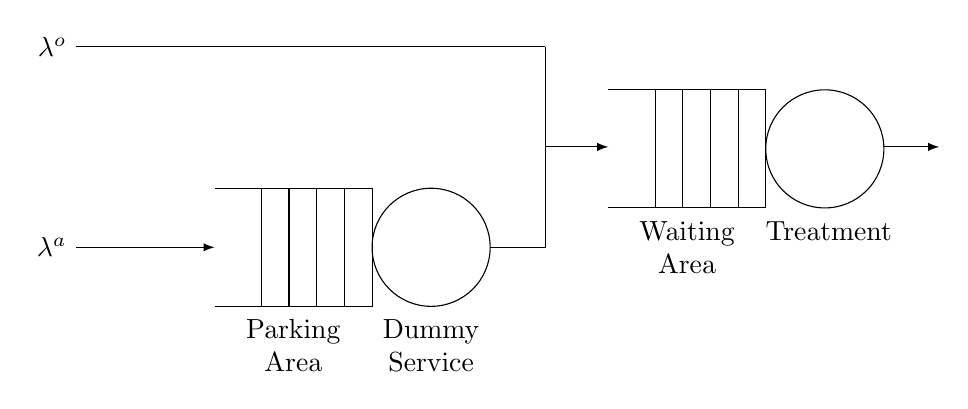
\begin{tikzpicture}[>=latex]
        % the rectangle with vertical rules (Queue 1)
        \draw (0,0) -- ++(2cm,0) -- ++(0,-1.5cm) -- ++(-2cm,0);
        \foreach \i in {1,...,4}
        \draw (2cm-\i*10pt,0) -- +(0,-1.5cm);
        
        % the circle (Queue 1)
        \draw (2.75,-0.75cm) circle [radius=0.75cm];

        % the rectangle with vertical rules (Queue 2)
        \draw (5,1.25) -- ++(2cm,0) -- ++(0,-1.5cm) -- ++(-2cm,0);
        \foreach \i in {1,...,4}
        \draw (7cm-\i*10pt,1.25) -- +(0,-1.5cm);

        % the circle (Queue 2)
        \draw (7.75,0.5) circle [radius=0.75cm];

        % the arrows and labels (Queue 1+2)
        \draw[-] (3.5,-0.75) -- +(20pt,0);
        \draw[<-] (0,-0.75) -- +(-50pt,0) node[left] {\( \lambda^a \)};
        \draw[->] (8.5,0.525) -- +(20pt,0);
        \node[align=center] at (1cm,-2cm) {Parking \\ Area};
        \node[align=center] at (2.75cm,-2cm) {Dummy \\ Service};
        \node[align=center] at (6cm,-0.75cm) {Waiting \\ Area};
        \node[align=center] at (7.8cm,-0.75cm) {Treatment \\ };
        
        \draw (4.2, 1.8) -- +(-169.5pt,0) node[left] {\( \lambda^o \)};
        \draw (4.2, 1.8) -- (4.2, -0.75);
        \draw[->] (4.2, 0.525) -- (5, 0.525);

    \end{tikzpicture}
\end{figure}


\begin{figure}
    \centering
    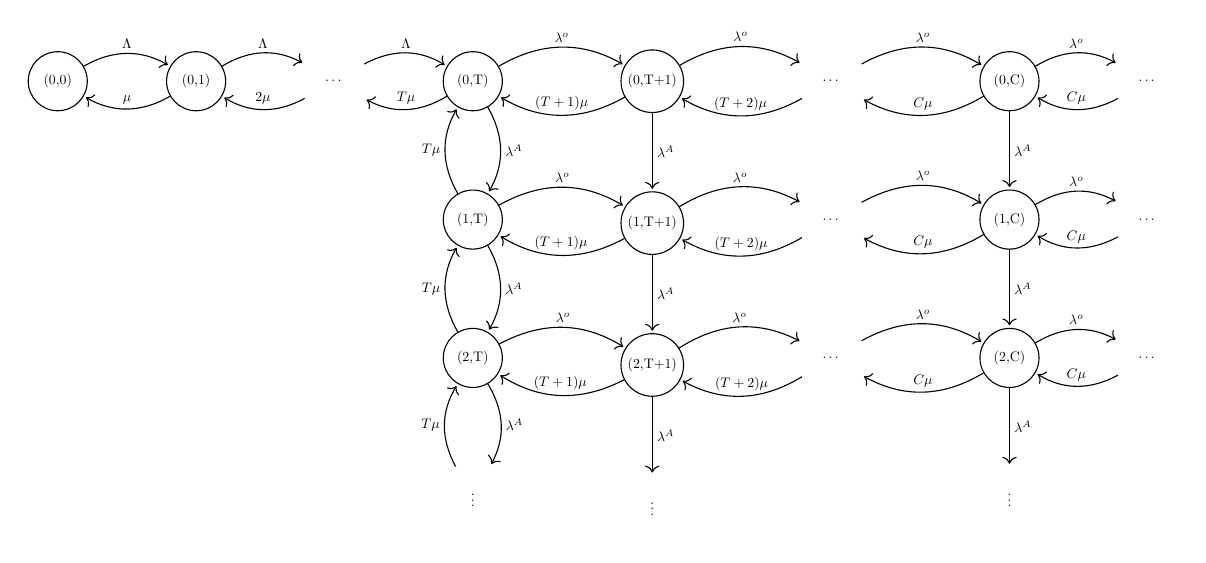
\begin{tikzpicture}[-, node distance = 1cm, auto, every node/.style={scale=0.5}]

        % Variables
        \tikzmath{
            let \altdist = 1.5cm;
            let \minsz = 1.5cm;
        }

        % First Line
        \node[state, minimum size=1.5cm] (zero) {(0,0)};
        \node[state, minimum size=1.5cm,  right=of zero] (one) {(0,1)};
        \node[draw=none, minimum size=1.5cm, right=of one] (two) {\dots};
        \node[state, minimum size=1.5cm, right=of two] (three) {(0,T)};
        \node[state, node distance = \altdist, minimum size=\minsz, right=of three] (four) {(0,T+1)};
        \node[draw=none, node distance = \altdist, minimum size=\minsz, right=of four] (five) {\dots};
        \node[state, node distance = \altdist, minimum size=\minsz, right=of five] (six) {(0,C)};
        \node[draw=none, minimum size=\minsz, right=of six] (seven) {\dots};

        % Second Line
        \node[state, minimum size=\minsz, below=of three] (three_one) {(1,T)};
        \node[state, minimum size=\minsz, below=of four] (four_one) {(1,T+1)};
        \node[draw=none, minimum size=\minsz, below=of five] (five_one) {\dots};
        \node[state, node distance = \altdist, minimum size=\minsz, right=of five_one] (six_one) {(1,C)};
        \node[draw=none, minimum size=\minsz, right=of six_one] (seven_one) {\dots};

        % Third Line
        \node[state, minimum size=\minsz, below=of three_one] (three_two) {(2,T)};
        \node[state, minimum size=\minsz, below=of four_one] (four_two) {(2,T+1)};
        \node[draw=none, minimum size=\minsz, below=of five_one] (five_two) {\dots};
        \node[state, node distance = \altdist, minimum size=\minsz, right=of five_two] (six_two) {(2,C)};
        \node[draw=none, minimum size=\minsz, right=of six_two] (seven_two) {\dots};

        % Fourth line
        \node[draw=none, minimum size=\minsz, below=of three_two] (three_three) {\vdots};
        \node[draw=none, minimum size=\minsz, below=of four_two] (four_three) {\vdots};
        \node[draw=none, minimum size=\minsz, below=of five_two] (five_three) {};
        \node[draw=none, node distance = \altdist, minimum size=\minsz, right=of five_three] (six_three) {\vdots};

        \draw[every loop]
            % First Horizontal Edges
            (zero) edge[bend left] node {\( \Lambda \)} (one)
            (one) edge[bend left] node [above] {\( \mu \)} (zero)
            (one) edge[bend left] node {\( \Lambda \)} (two)
            (two) edge[bend left] node [above] {\( 2 \mu \)} (one)
            (two) edge[bend left] node {\( \Lambda \)} (three)
            (three) edge[bend left] node [above] {\( T \mu \)} (two)
            (three) edge[bend left] node {\( \lambda^o \)} (four)
            (four) edge[bend left] node [above] {\( (T+1) \mu \)} (three)
            (four) edge[bend left] node {\( \lambda^o \)} (five)
            (five) edge[bend left] node [above] {\( (T+2) \mu \)} (four)
            (five) edge[bend left] node {\( \lambda^o \)} (six)
            (six) edge[bend left] node [above] {\( C\mu \)} (five)
            (six) edge[bend left] node {\( \lambda^o \)} (seven)
            (seven) edge[bend left] node [above] {\( C\mu \)} (six)

            % Second Horizontal Edges
            (three_one) edge[bend left] node {\( \lambda^o \)} (four_one)
            (four_one) edge[bend left] node [above] {\( (T+1) \mu \)} (three_one)
            (four_one) edge[bend left] node {\( \lambda^o \)} (five_one)
            (five_one) edge[bend left] node [above] {\( (T+2) \mu \)} (four_one)
            (five_one) edge[bend left] node {\( \lambda^o \)} (six_one)
            (six_one) edge[bend left] node [above] {\( C\mu \)} (five_one)
            (six_one) edge[bend left] node {\( \lambda^o \)} (seven_one)
            (seven_one) edge[bend left] node [above] {\( C\mu \)} (six_one)

            % Third Horizontal Edges
            (three_two) edge[bend left] node {\( \lambda^o \)} (four_two)
            (four_two) edge[bend left] node [above] {\( (T+1) \mu \)} (three_two)
            (four_two) edge[bend left] node {\( \lambda^o \)} (five_two)
            (five_two) edge[bend left] node [above] {\( (T+2) \mu \)} (four_two)
            (five_two) edge[bend left] node {\( \lambda^o \)} (six_two)
            (six_two) edge[bend left] node [above] {\( C\mu \)} (five_two)
            (six_two) edge[bend left] node {\( \lambda^o \)} (seven_two)
            (seven_two) edge[bend left] node [above] {\( C\mu \)} (six_two)

            % First Vertical Edges
            (three) edge[bend left] node {\( \lambda^A \)} (three_one)
            (three_one) edge[bend left] node {\( T \mu \)} (three)
            (three_one) edge[bend left] node {\( \lambda^A \)} (three_two)
            (three_two) edge[bend left] node {\( T\mu \)} (three_one)
            (three_two) edge[bend left] node {\( \lambda^A \)} (three_three)
            (three_three) edge[bend left] node {\( T\mu \)} (three_two)

            % Second Vertical Edges
            (four) edge node {\( \lambda^A \)} (four_one)
            (four_one) edge node {\( \lambda^A \)} (four_two)
            (four_two) edge node {\( \lambda^A \)} (four_three)

            %Third Vertical Edges
            (six) edge node {\( \lambda^A \)} (six_one)
            (six_one) edge node {\( \lambda^A \)} (six_two)
            (six_two) edge node {\( \lambda^A \)} (six_three)
            ;       
    \end{tikzpicture}
    \caption{Markov chains} 
    \label{Markov_2}
\end{figure}



\begin{figure}
    \centering
    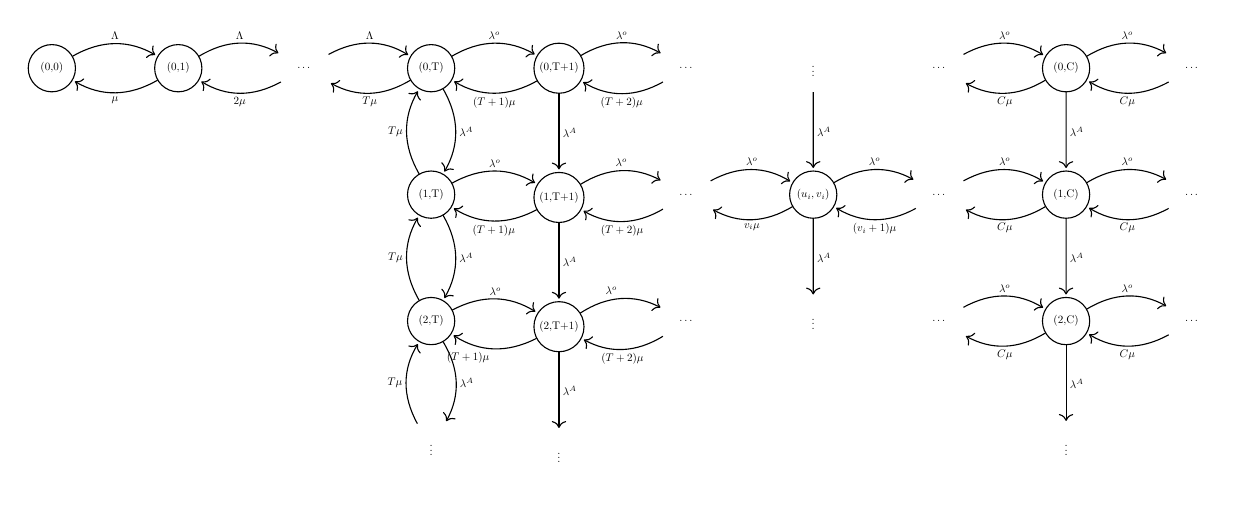
\begin{tikzpicture}[-, node distance = 1cm, auto, every node/.style={scale=0.4}]

        % Variables
        \tikzmath{
            let \altdist = 1cm;
            let \minsz = 1.5cm;
        }

        % First Line
        \node[state, minimum size=1.5cm] (zero) {(0,0)};
        \node[state, minimum size=1.5cm,  right=of zero] (one) {(0,1)};
        \node[draw=none, minimum size=1.5cm, right=of one] (two) {\dots};
        \node[state, minimum size=1.5cm, right=of two] (three) {(0,T)};
        \node[state, node distance = \altdist, minimum size=\minsz, right=of three] (four) {(0,T+1)};
        \node[draw=none, minimum size=\minsz, right=of four] (five) {\dots};
        \node[draw=none, minimum size=\minsz, right=of five] (six) {\vdots};
        \node[draw=none, minimum size=\minsz, right=of six] (seven) {\dots};
        \node[state, minimum size=\minsz, right=of seven] (eight) {(0,C)};
        \node[draw=none, minimum size=\minsz, right=of eight] (nine) {\dots};


        % Second Line
        \node[state, minimum size=\minsz, below=of three] (three_one) {(1,T)};
        \node[state, minimum size=\minsz, below=of four] (four_one) {(1,T+1)};
        \node[draw=none, minimum size=\minsz, below=of five] (five_one) {\dots};
        \node[state, node distance = \altdist, minimum size=\minsz, right=of five_one] (six_one) {\( (u_i, v_i) \)};
        \node[draw=none, minimum size=\minsz, right=of six_one] (seven_one) {\dots};
        \node[state, node distance = \altdist, minimum size=\minsz, right=of seven_one] (eight_one) {(1,C)};
        \node[draw=none, minimum size=\minsz, right=of eight_one] (nine_one) {\dots};
        

        % Third Line
        \node[state, minimum size=\minsz, below=of three_one] (three_two) {(2,T)};
        \node[state, minimum size=\minsz, below=of four_one] (four_two) {(2,T+1)};
        \node[draw=none, minimum size=\minsz, below=of five_one] (five_two) {\dots};
        \node[draw=none, node distance = \altdist, minimum size=\minsz, right=of five_two] (six_two) {\vdots};
        \node[draw=none, minimum size=\minsz, right=of six_two] (seven_two) {\dots};
        \node[state, node distance = \altdist, minimum size=\minsz, right=of seven_two] (eight_two) {(2,C)};
        \node[draw=none, minimum size=\minsz, right=of eight_two] (nine_two) {\dots};

        % Fourth line
        \node[draw=none, minimum size=\minsz, below=of three_two] (three_three) {\vdots};
        \node[draw=none, minimum size=\minsz, below=of four_two] (four_three) {\vdots};
        \node[draw=none, minimum size=\minsz, below=of five_two] (five_three) {};
        \node[draw=none, node distance = \altdist, minimum size=\minsz, right=of five_three] (six_three) {};
        \node[draw=none, node distance = \altdist, minimum size=\minsz, below=of eight_two] (eight_three) {\vdots};


        \draw[every loop]
            % First Horizontal Edges
            (zero) edge[bend left] node {\( \Lambda \)} (one)
            (one) edge[bend left] node {\( \mu \)} (zero)
            (one) edge[bend left] node {\( \Lambda \)} (two)
            (two) edge[bend left] node {\( 2 \mu \)} (one)
            (two) edge[bend left] node {\( \Lambda \)} (three)
            (three) edge[bend left] node {\( T \mu \)} (two)
            (three) edge[bend left] node {\( \lambda^o \)} (four)
            (four) edge[bend left] node {\( (T+1) \mu \)} (three)
            (four) edge[bend left] node {\( \lambda^o \)} (five)
            (five) edge[bend left] node {\( (T+2) \mu \)} (four)
            % (five) edge[bend left] node {\( \lambda^o \)} (six)
            % (six) edge[bend left] node [above] {\( C\mu \)} (five)
            % (six) edge[bend left] node {\( \lambda^o \)} (seven)
            % (seven) edge[bend left] node [above] {\( C\mu \)} (six)
            (seven) edge[bend left] node {\( \lambda^o \)} (eight)
            (eight) edge[bend left] node {\( C\mu \)} (seven)
            (eight) edge[bend left] node {\( \lambda^o \)} (nine)
            (nine) edge[bend left] node {\( C\mu \)} (eight)

            % Second Horizontal Edges
            (three_one) edge[bend left] node {\(\lambda^o\)} (four_one)
            (four_one) edge[bend left] node {\( (T+1) \mu \)} (three_one)
            (four_one) edge[bend left] node {\( \lambda^o \)} (five_one)
            (five_one) edge[bend left] node {\( (T+2) \mu \)} (four_one)
            (five_one) edge[bend left] node {\( \lambda^o \)} (six_one)
            (six_one) edge[bend left] node {\( v_i\mu \)} (five_one)
            (six_one) edge[bend left] node {\( \lambda^o \)} (seven_one)
            (seven_one) edge[bend left] node {\( (v_i+1)\mu \)} (six_one)
            (seven_one) edge[bend left] node {\( \lambda^o \)} (eight_one)
            (eight_one) edge[bend left] node {\( C\mu \)} (seven_one)
            (eight_one) edge[bend left] node {\( \lambda^o \)} (nine_one)
            (nine_one) edge[bend left] node {\( C\mu \)} (eight_one)

            % Third Horizontal Edges
            (three_two) edge[bend left] node {\( \lambda^o \)} (four_two)
            (four_two) edge[bend left] node {\( (T+1) \mu \)} (three_two)
            (four_two) edge[bend left] node {\( \lambda^o \)} (five_two)
            (five_two) edge[bend left] node {\( (T+2) \mu \)} (four_two)
            % (five_two) edge[bend left] node {\( \lambda^o \)} (six_two)
            % (six_two) edge[bend left] node [above] {\( C\mu \)} (five_two)
            % (six_two) edge[bend left] node {\( \lambda^o \)} (seven_two)
            % (seven_two) edge[bend left] node [above] {\( C\mu \)} (six_two)
            (seven_two) edge[bend left] node {\( \lambda^o \)} (eight_two)
            (eight_two) edge[bend left] node {\( C\mu \)} (seven_two)
            (eight_two) edge[bend left] node {\( \lambda^o \)} (nine_two)
            (nine_two) edge[bend left] node {\( C\mu \)} (eight_two)

            % First Vertical Edges
            (three) edge[bend left] node {\( \lambda^A \)} (three_one)
            (three_one) edge[bend left] node {\( T \mu \)} (three)
            (three_one) edge[bend left] node {\( \lambda^A \)} (three_two)
            (three_two) edge[bend left] node {\( T\mu \)} (three_one)
            (three_two) edge[bend left] node {\( \lambda^A \)} (three_three)
            (three_three) edge[bend left] node {\( T\mu \)} (three_two)

            % Second Vertical Edges
            (four) edge node {\( \lambda^A \)} (four_one)
            (four_one) edge node {\( \lambda^A \)} (four_two)
            (four_two) edge node {\( \lambda^A \)} (four_three)

            % Third Vertical Edges
            (six) edge node {\( \lambda^A \)} (six_one)
            (six_one) edge node {\( \lambda^A \)} (six_two)
            % (six_two) edge node {\( \lambda^A \)} (six_three)

            % Fourth Vertical Edges
            (eight) edge node {\( \lambda^A \)} (eight_one)
            (eight_one) edge node {\( \lambda^A \)} (eight_two)
            (eight_two) edge node {\( \lambda^A \)} (eight_three)
            ;       
    \end{tikzpicture}
    \caption{Markov chains} 
    \label{Markov_3}
\end{figure}


\begin{figure}
    \centering
    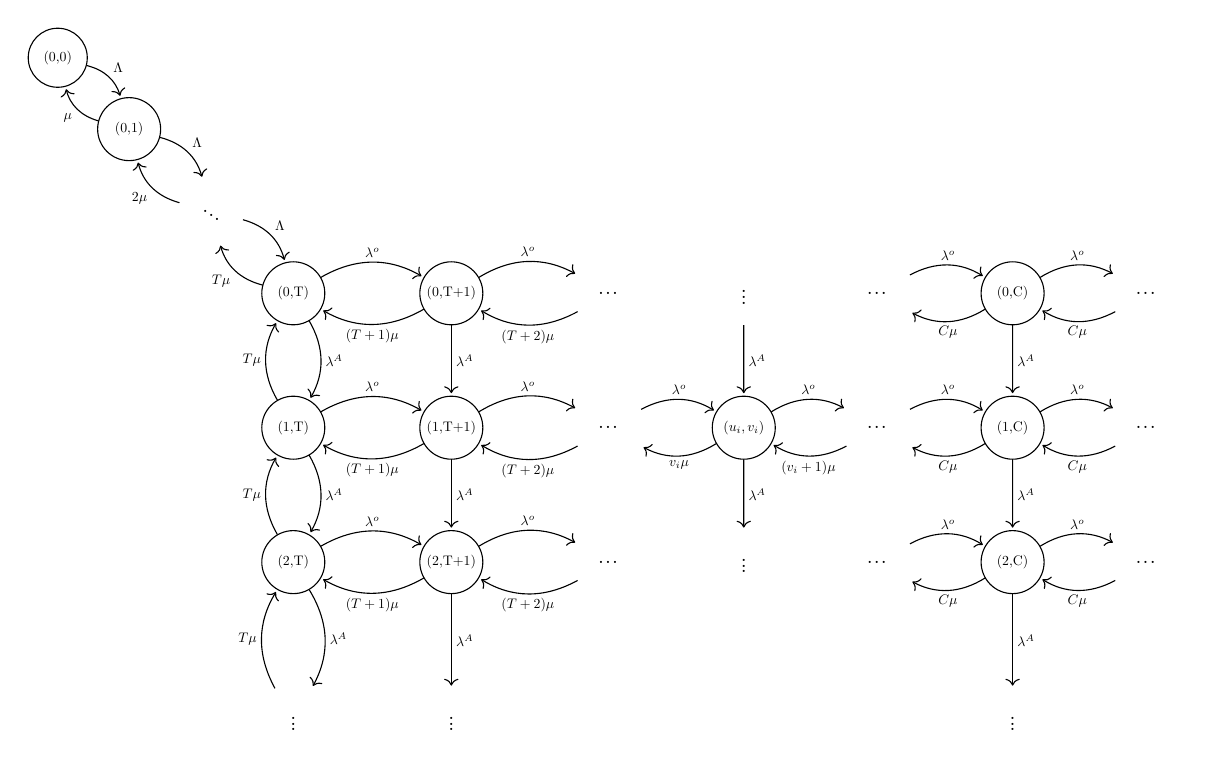
\begin{tikzpicture}[-, node distance = 0.9cm, auto, every node/.style={scale=0.5}]

        % Variables
        \tikzmath{
            let \initdist = 0.5cm;
            let \altdist = 1.2cm;
            let \minsz = 1.6cm;
            let \leftOne = -0.8;
            let \rightOne = 2.2;
            let \upOne = 0.8;
            let \downOne = -2.2;
            let \leftTwo = 2.25;
            let \rightTwo = 14.2;
            let \upTwo = -2.35;
            let \downTwo = -8.8;
        }

        % % Rectangle for S1
        % \draw[ultra thin, dashed] (\leftOne, \downOne) -- (\leftOne, \upOne);
        % \draw[ultra thin, dashed] (\leftOne, \upOne) -- (\rightOne, \upOne);
        % \draw[ultra thin, dashed] (\rightOne, \upOne) -- node {\Huge{\( \quad S_1 \)}}(\rightOne, \downOne);
        % \draw[ultra thin, dashed] (\rightOne, \downOne) -- (\leftOne, \downOne);

        % % Rectangle for S2
        % \draw[ultra thin, dashed] (\leftTwo, \downTwo) -- node {\Huge{\( S_2 \quad \)}}(\leftTwo, \upTwo);
        % \draw[ultra thin, dashed] (\leftTwo, \upTwo) -- (\rightTwo, \upTwo);
        % \draw[ultra thin, dashed] (\rightTwo, \upTwo) -- (\rightTwo, \downTwo);
        % \draw[ultra thin, dashed] (\rightTwo, \downTwo) -- (\leftTwo, \downTwo);

        % First Line
        \node[state, minimum size=1.5cm] (zero) {(0,0)};
        \node[state, node distance = \initdist, minimum size=\minsz, below right=of zero] (one) {(0,1)};
        \node[draw=none, node distance = \initdist, minimum size=\minsz, below right=of one] (two) {\textbf{\( \ddots \)}};
        \node[state, node distance = \initdist, minimum size=\minsz, below right=of two] (three) {(0,T)};
        \node[state, node distance = \altdist, minimum size=\minsz, right=of three] (four) {(0,T+1)};
        \node[draw=none, node distance = \altdist, minimum size=\minsz, right=of four] (five) {\textbf{\dots}};
        \node[draw=none, minimum size=\minsz, right=of five] (six) {\textbf{\vdots}};
        \node[draw=none, minimum size=\minsz, right=of six] (seven) {\textbf{\dots}};
        \node[state, minimum size=\minsz, right=of seven] (eight) {(0,C)};
        \node[draw=none, minimum size=\minsz, right=of eight] (nine) {\textbf{\dots}};


        % Second Line
        \node[state, minimum size=\minsz, below=of three] (three_one) {(1,T)};
        \node[state, minimum size=\minsz, below=of four] (four_one) {(1,T+1)};
        \node[draw=none, minimum size=\minsz, below=of five] (five_one) {\textbf{\dots}};
        \node[state, minimum size=\minsz, right=of five_one] (six_one) {\( (u_i, v_i) \)};
        \node[draw=none, minimum size=\minsz, right=of six_one] (seven_one) {\textbf{\dots}};
        \node[state, minimum size=\minsz, right=of seven_one] (eight_one) {(1,C)};
        \node[draw=none, minimum size=\minsz, right=of eight_one] (nine_one) {\textbf{\dots}};
        

        % Third Line
        \node[state, minimum size=\minsz, below=of three_one] (three_two) {(2,T)};
        \node[state, minimum size=\minsz, below=of four_one] (four_two) {(2,T+1)};
        \node[draw=none, minimum size=\minsz, below=of five_one] (five_two) {\textbf{\dots}};
        \node[draw=none, minimum size=\minsz, right=of five_two] (six_two) {\textbf{\vdots}};
        \node[draw=none, minimum size=\minsz, right=of six_two] (seven_two) {\textbf{\dots}};
        \node[state, minimum size=\minsz, right=of seven_two] (eight_two) {(2,C)};
        \node[draw=none, minimum size=\minsz, right=of eight_two] (nine_two) {\textbf{\dots}};

        % Fourth line
        \node[draw=none, node distance = \altdist, minimum size=\minsz, below=of three_two] (three_three) {\textbf{\vdots}};
        \node[draw=none, node distance = \altdist, minimum size=\minsz, below=of four_two] (four_three) {\textbf{\vdots}};
        \node[draw=none, node distance = \altdist, minimum size=\minsz, below=of five_two] (five_three) {};
        \node[draw=none, node distance = \altdist, minimum size=\minsz, below=of six_two] (six_three) {};
        \node[draw=none, node distance = \altdist, minimum size=\minsz, below=of eight_two] (eight_three) {\textbf{\vdots}};


        \draw[every loop]
            % First Horizontal Edges
            (zero) edge[bend left] node {\( \Lambda \)} (one)
            (one) edge[bend left] node {\( \mu \)} (zero)
            (one) edge[bend left] node {\( \Lambda \)} (two)
            (two) edge[bend left] node {\( 2 \mu \)} (one)
            (two) edge[bend left] node {\( \Lambda \)} (three)
            (three) edge[bend left] node {\( T \mu \)} (two)
            (three) edge[bend left] node {\( \lambda^o \)} (four)
            (four) edge[bend left] node {\( (T+1) \mu \)} (three)
            (four) edge[bend left] node {\( \lambda^o \)} (five)
            (five) edge[bend left] node {\( (T+2) \mu \)} (four)
            % (five) edge[bend left] node {\( \lambda^o \)} (six)
            % (six) edge[bend left] node [above] {\( C\mu \)} (five)
            % (six) edge[bend left] node {\( \lambda^o \)} (seven)
            % (seven) edge[bend left] node [above] {\( C\mu \)} (six)
            (seven) edge[bend left] node {\( \lambda^o \)} (eight)
            (eight) edge[bend left] node {\( C\mu \)} (seven)
            (eight) edge[bend left] node {\( \lambda^o \)} (nine)
            (nine) edge[bend left] node {\( C\mu \)} (eight)

            % Second Horizontal Edges
            (three_one) edge[bend left] node {\( \lambda^o \)} (four_one)
            (four_one) edge[bend left] node {\( (T+1) \mu \)} (three_one)
            (four_one) edge[bend left] node {\( \lambda^o \)} (five_one)
            (five_one) edge[bend left] node {\( (T+2) \mu \)} (four_one)
            (five_one) edge[bend left] node {\( \lambda^o \)} (six_one)
            (six_one) edge[bend left] node {\( v_i\mu \)} (five_one)
            (six_one) edge[bend left] node {\( \lambda^o \)} (seven_one)
            (seven_one) edge[bend left] node {\( (v_i+1)\mu \)} (six_one)
            (seven_one) edge[bend left] node {\( \lambda^o \)} (eight_one)
            (eight_one) edge[bend left] node {\( C\mu \)} (seven_one)
            (eight_one) edge[bend left] node {\( \lambda^o \)} (nine_one)
            (nine_one) edge[bend left] node {\( C\mu \)} (eight_one)

            % Third Horizontal Edges
            (three_two) edge[bend left] node {\( \lambda^o \)} (four_two)
            (four_two) edge[bend left] node [below] {\( (T+1) \mu \)} (three_two)
            (four_two) edge[bend left] node {\( \lambda^o \)} (five_two)
            (five_two) edge[bend left] node {\( (T+2) \mu \)} (four_two)
            % (five_two) edge[bend left] node {\( \lambda^o \)} (six_two)
            % (six_two) edge[bend left] node [above] {\( C\mu \)} (five_two)
            % (six_two) edge[bend left] node {\( \lambda^o \)} (seven_two)
            % (seven_two) edge[bend left] node [above] {\( C\mu \)} (six_two)
            (seven_two) edge[bend left] node {\( \lambda^o \)} (eight_two)
            (eight_two) edge[bend left] node {\( C\mu \)} (seven_two)
            (eight_two) edge[bend left] node {\( \lambda^o \)} (nine_two)
            (nine_two) edge[bend left] node {\( C\mu \)} (eight_two)

            % First Vertical Edges
            (three) edge[bend left] node {\( \lambda^A \)} (three_one)
            (three_one) edge[bend left] node {\( T \mu \)} (three)
            (three_one) edge[bend left] node {\( \lambda^A \)} (three_two)
            (three_two) edge[bend left] node {\( T\mu \)} (three_one)
            (three_two) edge[bend left] node {\( \lambda^A \)} (three_three)
            (three_three) edge[bend left] node {\( T\mu \)} (three_two)

            % Second Vertical Edges
            (four) edge node {\( \lambda^A \)} (four_one)
            (four_one) edge node {\( \lambda^A \)} (four_two)
            (four_two) edge node {\( \lambda^A \)} (four_three)

            % Third Vertical Edges
            (six) edge node {\( \lambda^A \)} (six_one)
            (six_one) edge node {\( \lambda^A \)} (six_two)
            % (six_two) edge node {\( \lambda^A \)} (six_three)

            % Fourth Vertical Edges
            (eight) edge node {\( \lambda^A \)} (eight_one)
            (eight_one) edge node {\( \lambda^A \)} (eight_two)
            (eight_two) edge node {\( \lambda^A \)} (eight_three)
            ;       
    \end{tikzpicture}
    \caption{Markov chains} 
    \label{Markov_4}
\end{figure}




\begin{figure}
    \centering
    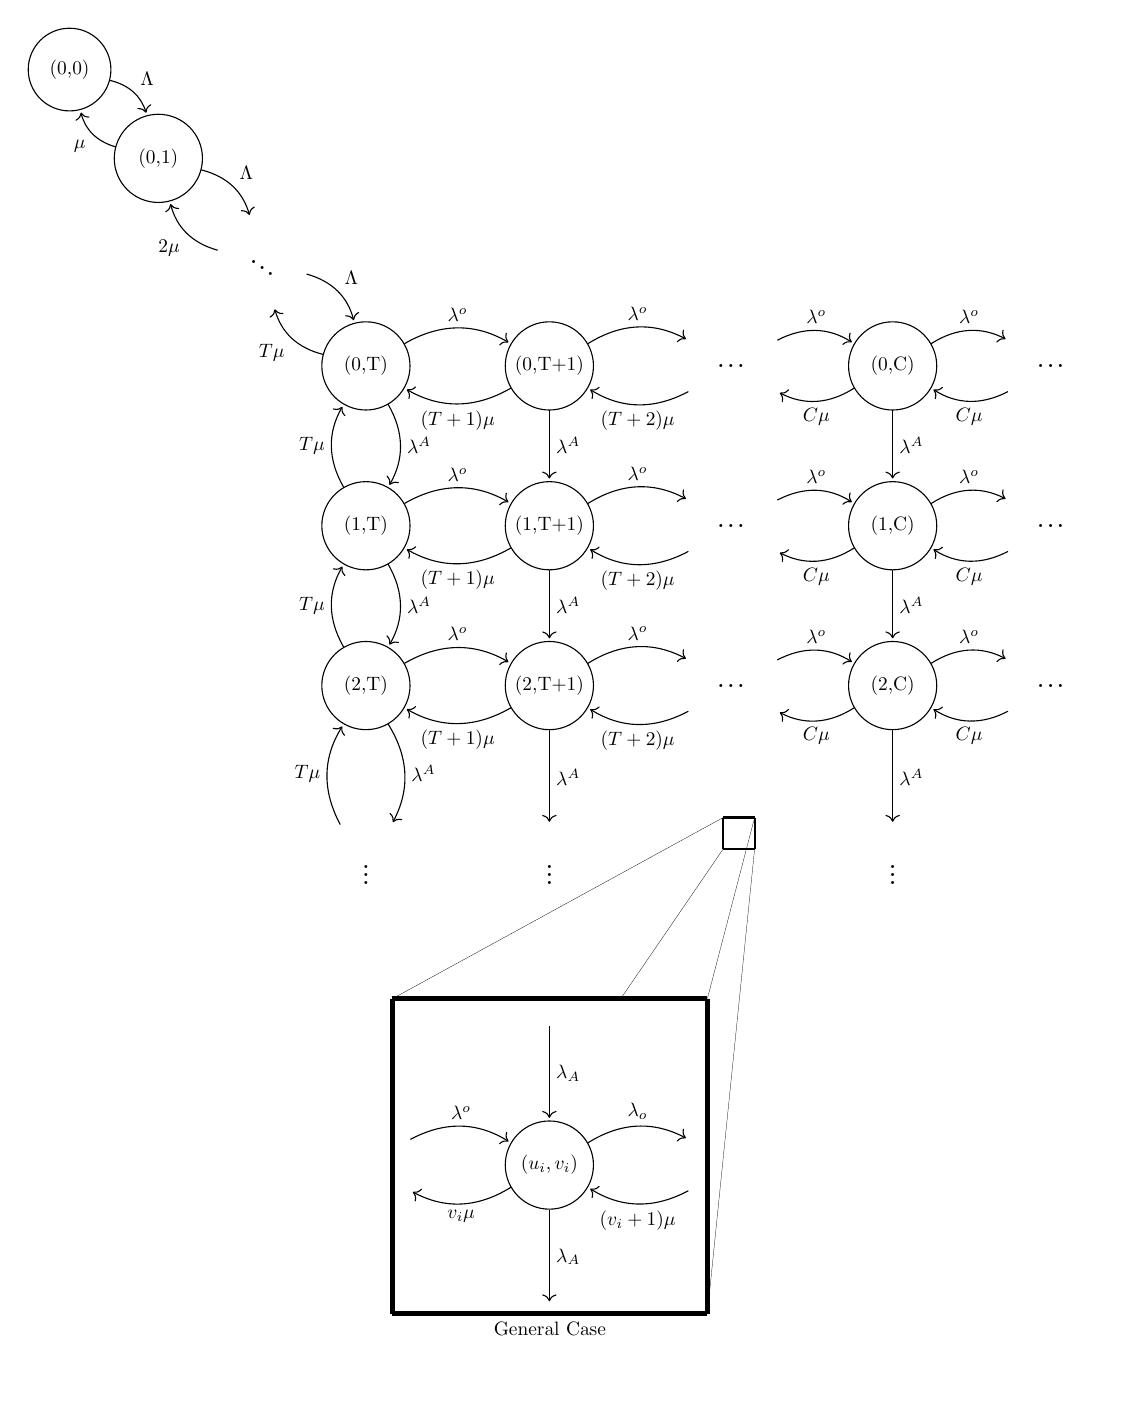
\begin{tikzpicture}[-, node distance = 0.9cm, auto, every node/.style={scale=0.7}]

        % Markov chain variables
        \tikzmath{
            let \initdist = 0.5cm;
            let \altdist = 1.2cm;
            let \minsz = 1.6cm;
        }

        % S_1 and S_2 rectangles
        \tikzmath{
            let \leftOne = -0.8;
            let \rightOne = 2.7;
            let \upOne = 0.8;
            let \downOne = -2.7;
            let \leftTwo = 2.8;
            let \rightTwo = 13;
            let \upTwo = -2.95;
            let \downTwo = -16.4;
        }

        % General case variables
        \tikzmath{
            let \GCsmallx = 8.3;
            let \GCsmally = -9.5;
            let \GCbigx = 4.1;
            let \GCbigy = -11.8;
        }

        % % Rectangle for S1
        % \draw[ultra thin, dashed] (\leftOne, \downOne) -- (\leftOne, \upOne);
        % \draw[ultra thin, dashed] (\leftOne, \upOne) -- (\rightOne, \upOne);
        % \draw[ultra thin, dashed] (\rightOne, \upOne) -- node {\Huge{\( \quad S_1 \)}}(\rightOne, \downOne);
        % \draw[ultra thin, dashed] (\rightOne, \downOne) -- (\leftOne, \downOne);

        % % Rectangle for S2
        % \draw[ultra thin, dashed] (\leftTwo, \downTwo) -- node {\Huge{\( S_2 \quad \)}}(\leftTwo, \upTwo);
        % \draw[ultra thin, dashed] (\leftTwo, \upTwo) -- (\rightTwo, \upTwo);
        % \draw[ultra thin, dashed] (\rightTwo, \upTwo) -- (\rightTwo, \downTwo);
        % \draw[ultra thin, dashed] (\rightTwo, \downTwo) -- (\leftTwo, \downTwo);

        % Small square of general case
        \draw [thick] (\GCsmallx, \GCsmally) -- node {} (\GCsmallx + 0.4, \GCsmally);
        \draw [thick] (\GCsmallx + 0.4, \GCsmally) -- node {} (\GCsmallx + 0.4, \GCsmally - 0.4);
        \draw [thick] (\GCsmallx + 0.4, \GCsmally - 0.4) -- node {} (\GCsmallx, \GCsmally - 0.4);
        \draw [thick] (\GCsmallx, \GCsmally - 0.4) -- node {} (\GCsmallx, \GCsmally);


        % Dashed lines to from small square to big one 
        \draw [ultra thin] (\GCsmallx, \GCsmally) -- node {} (\GCbigx, \GCbigy);
        \draw [ultra thin] (\GCsmallx + 0.4, \GCsmally) -- node {} (\GCbigx + 4, \GCbigy);
        \draw [ultra thin] (\GCsmallx, \GCsmally - 0.4) -- node {} (7, \GCbigy);
        \draw [ultra thin] (\GCsmallx + 0.4, \GCsmally - 0.4) -- node {} (\GCbigx + 4, \GCbigy - 4);
        
        % Big Square of general case
        \draw [ultra thick] (\GCbigx, \GCbigy) -- node {} (\GCbigx + 4, \GCbigy);
        \draw [ultra thick] (\GCbigx + 4, \GCbigy) -- node {} (\GCbigx + 4, \GCbigy - 4);
        \draw [ultra thick] (\GCbigx + 4, \GCbigy - 4) -- node {General Case} (\GCbigx, \GCbigy - 4);
        \draw [ultra thick] (\GCbigx, \GCbigy - 4) -- node {} (\GCbigx, \GCbigy);

        % First Line
        \node[state, minimum size=1.5cm] (zero) {(0,0)};
        \node[state, node distance = \initdist, minimum size=\minsz, below right=of zero] (one) {(0,1)};
        \node[draw=none, node distance = \initdist, minimum size=\minsz, below right=of one] (two) {\textbf{\( \ddots \)}};
        \node[state, node distance = \initdist, minimum size=\minsz, below right=of two] (three) {(0,T)};
        \node[state, node distance = \altdist, minimum size=\minsz, right=of three] (four) {(0,T+1)};
        \node[draw=none, node distance = \altdist, minimum size=\minsz, right=of four] (five) {\textbf{\dots}};
        \node[state, minimum size=\minsz, right=of five] (six) {(0,C)};
        \node[draw=none, minimum size=\minsz, right=of six] (seven) {\textbf{\dots}};

        % Second Line
        \node[state, minimum size=\minsz, below=of three] (three_one) {(1,T)};
        \node[state, minimum size=\minsz, below=of four] (four_one) {(1,T+1)};
        \node[draw=none, minimum size=\minsz, below=of five] (five_one) {\textbf{\dots}};
        \node[state, minimum size=\minsz, right=of five_one] (six_one) {(1,C)};
        \node[draw=none, minimum size=\minsz, right=of six_one] (seven_one) {\textbf{\dots}};
        
        % Third Line
        \node[state, minimum size=\minsz, below=of three_one] (three_two) {(2,T)};
        \node[state, minimum size=\minsz, below=of four_one] (four_two) {(2,T+1)};
        \node[draw=none, minimum size=\minsz, below=of five_one] (five_two) {\textbf{\dots}};
        \node[state, minimum size=\minsz, right=of five_two] (six_two) {(2,C)};
        \node[draw=none, minimum size=\minsz, right=of six_two] (seven_two) {\textbf{\dots}};

        % Fourth line
        \node[draw=none, node distance = \altdist, minimum size=\minsz, below=of three_two] (three_three) {\textbf{\vdots}};
        \node[draw=none, node distance = \altdist, minimum size=\minsz, below=of four_two] (four_three) {\textbf{\vdots}};
        \node[draw=none, node distance = 2cm, minimum size=\minsz, below=of five_two] (five_three) {};
        \node[draw=none, node distance = \altdist, minimum size=\minsz, below=of six_two] (six_three) {\textbf{\vdots}};

        % Fifth line
        % \node[state, node distance = \altdist, minimum size=\minsz, below=of five_three] (general_case_mid) {\( (u_i, v_i) \)};
        \node[draw=none, node distance = 0.3cm, minimum size=\minsz, below=of four_three] (general_case_up) {};
        \node[state, node distance = \altdist, minimum size=\minsz, below=of general_case_up] (general_case_mid) {\( (u_i, v_i) \)};

        \node[draw=none, node distance = \altdist, minimum size=\minsz, below=of general_case_mid] (general_case_down) {};
        \node[draw=none, node distance = \altdist, minimum size=\minsz, left=of general_case_mid] (general_case_left) {};
        \node[draw=none, node distance = \altdist, minimum size=\minsz, right=of general_case_mid] (general_case_right) {};

        \draw[every loop]
            % First Horizontal Edges
            (zero) edge[bend left] node {\( \Lambda \)} (one)
            (one) edge[bend left] node {\( \mu \)} (zero)
            (one) edge[bend left] node {\( \Lambda \)} (two)
            (two) edge[bend left] node {\( 2 \mu \)} (one)
            (two) edge[bend left] node {\( \Lambda \)} (three)
            (three) edge[bend left] node {\( T \mu \)} (two)
            (three) edge[bend left] node {\( \lambda^o \)} (four)
            (four) edge[bend left] node {\( (T+1) \mu \)} (three)
            (four) edge[bend left] node {\( \lambda^o \)} (five)
            (five) edge[bend left] node {\( (T+2) \mu \)} (four)
            (five) edge[bend left] node {\( \lambda^o \)} (six)
            (six) edge[bend left] node {\( C\mu \)} (five)
            (six) edge[bend left] node {\( \lambda^o \)} (seven)
            (seven) edge[bend left] node {\( C\mu \)} (six)

            % Second Horizontal Edges
            (three_one) edge[bend left] node {\( \lambda^o \)} (four_one)
            (four_one) edge[bend left] node {\( (T+1) \mu \)} (three_one)
            (four_one) edge[bend left] node {\( \lambda^o \)} (five_one)
            (five_one) edge[bend left] node {\( (T+2) \mu \)} (four_one)
            (five_one) edge[bend left] node {\( \lambda^o \)} (six_one)
            (six_one) edge[bend left] node {\( C\mu \)} (five_one)
            (six_one) edge[bend left] node {\( \lambda^o \)} (seven_one)
            (seven_one) edge[bend left] node {\( C\mu \)} (six_one)

            % Third Horizontal Edges
            (three_two) edge[bend left] node {\( \lambda^o \)} (four_two)
            (four_two) edge[bend left] node [below] {\( (T+1) \mu \)} (three_two)
            (four_two) edge[bend left] node {\( \lambda^o \)} (five_two)
            (five_two) edge[bend left] node {\( (T+2) \mu \)} (four_two)
            (five_two) edge[bend left] node {\( \lambda^o \)} (six_two)
            (six_two) edge[bend left] node {\( C\mu \)} (five_two)
            (six_two) edge[bend left] node {\( \lambda^o \)} (seven_two)
            (seven_two) edge[bend left] node {\( C\mu \)} (six_two)

            % First Vertical Edges
            (three) edge[bend left] node {\( \lambda^A \)} (three_one)
            (three_one) edge[bend left] node {\( T \mu \)} (three)
            (three_one) edge[bend left] node {\( \lambda^A \)} (three_two)
            (three_two) edge[bend left] node {\( T\mu \)} (three_one)
            (three_two) edge[bend left] node {\( \lambda^A \)} (three_three)
            (three_three) edge[bend left] node {\( T\mu \)} (three_two)

            % Second Vertical Edges
            (four) edge node {\( \lambda^A \)} (four_one)
            (four_one) edge node {\( \lambda^A \)} (four_two)
            (four_two) edge node {\( \lambda^A \)} (four_three)

            % Fourth Vertical Edges
            (six) edge node {\( \lambda^A \)} (six_one)
            (six_one) edge node {\( \lambda^A \)} (six_two)
            (six_two) edge node {\( \lambda^A \)} (six_three)

            % General Case
            (general_case_left) edge[bend left] node {\( \lambda^o \)} (general_case_mid)
            (general_case_mid) edge[bend left] node {\( v_i \mu \)} (general_case_left)
            (general_case_right) edge[bend left] node {\( (v_i +1) \mu \)} (general_case_mid)
            (general_case_mid) edge[bend left] node {\( \lambda_o \)} (general_case_right)
            % (five_three) edge node {\( \lambda_A \)} (general_case_mid)
            (general_case_up) edge node {\( \lambda_A \)} (general_case_mid)
            (general_case_mid) edge node {\( \lambda_A \)} (general_case_down)
            ;
    \end{tikzpicture}
    \caption{Markov chain} 
    \label{Markov_5}
\end{figure}




% Formulas used
\newpage
\section{Figures that might be useful}
\begin{figure}[h]
    \centering
    \begin{tikzpicture}[>=latex]
        % the rectangle with vertical rules (Queue 1)
        \draw (0,0) -- ++(2cm,0) -- ++(0,-1.5cm) -- ++(-2cm,0);
        \foreach \i in {1,...,4}
        \draw (2cm-\i*10pt,0) -- +(0,-1.5cm);
        
        % the circle (Queue 1)
        \draw (2.75,-0.75cm) circle [radius=0.75cm];

        % the rectangle with vertical rules (Queue 2)
        \draw (5,1.25) -- ++(2cm,0) -- ++(0,-1.5cm) -- ++(-2cm,0);
        \foreach \i in {1,...,4}
        \draw (7cm-\i*10pt,1.25) -- +(0,-1.5cm);

        % the circle (Queue 2)
        \draw (7.75,0.5) circle [radius=0.75cm];

        % the arrows and labels (Queue 1+2)
        \draw[-] (3.5,-0.75) -- +(20pt,0);
        \draw[<-] (0,-0.75) -- +(-50pt,0) node[left] {\( \lambda^a \)};
        \draw[->] (8.5,0.525) -- +(20pt,0);
        \node[align=center] at (1cm,-2cm) {Parking \\ Area};
        \node[align=center] at (2.75cm,-2cm) {Dummy \\ Service};
        \node[align=center] at (6cm,-0.75cm) {Waiting \\ Area};
        \node[align=center] at (7.8cm,-0.75cm) {Treatment \\ };
        
        \draw (4.2, 1.8) -- +(-169.5pt,0) node[left] {\( \lambda^o \)};
        \draw (4.2, 1.8) -- (4.2, -0.75);
        \draw[->] (4.2, 0.525) -- (5, 0.525);

    \end{tikzpicture}
\end{figure}


\begin{figure}
    \centering
    \begin{tikzpicture}[-, node distance = 1cm, auto, every node/.style={scale=0.5}]

        % Variables
        \tikzmath{
            let \altdist = 1.5cm;
            let \minsz = 1.5cm;
        }

        % First Line
        \node[state, minimum size=1.5cm] (zero) {(0,0)};
        \node[state, minimum size=1.5cm,  right=of zero] (one) {(0,1)};
        \node[draw=none, minimum size=1.5cm, right=of one] (two) {\dots};
        \node[state, minimum size=1.5cm, right=of two] (three) {(0,T)};
        \node[state, node distance = \altdist, minimum size=\minsz, right=of three] (four) {(0,T+1)};
        \node[draw=none, node distance = \altdist, minimum size=\minsz, right=of four] (five) {\dots};
        \node[state, node distance = \altdist, minimum size=\minsz, right=of five] (six) {(0,C)};
        \node[draw=none, minimum size=\minsz, right=of six] (seven) {\dots};

        % Second Line
        \node[state, minimum size=\minsz, below=of three] (three_one) {(1,T)};
        \node[state, minimum size=\minsz, below=of four] (four_one) {(1,T+1)};
        \node[draw=none, minimum size=\minsz, below=of five] (five_one) {\dots};
        \node[state, node distance = \altdist, minimum size=\minsz, right=of five_one] (six_one) {(1,C)};
        \node[draw=none, minimum size=\minsz, right=of six_one] (seven_one) {\dots};

        % Third Line
        \node[state, minimum size=\minsz, below=of three_one] (three_two) {(2,T)};
        \node[state, minimum size=\minsz, below=of four_one] (four_two) {(2,T+1)};
        \node[draw=none, minimum size=\minsz, below=of five_one] (five_two) {\dots};
        \node[state, node distance = \altdist, minimum size=\minsz, right=of five_two] (six_two) {(2,C)};
        \node[draw=none, minimum size=\minsz, right=of six_two] (seven_two) {\dots};

        % Fourth line
        \node[draw=none, minimum size=\minsz, below=of three_two] (three_three) {\vdots};
        \node[draw=none, minimum size=\minsz, below=of four_two] (four_three) {\vdots};
        \node[draw=none, minimum size=\minsz, below=of five_two] (five_three) {};
        \node[draw=none, node distance = \altdist, minimum size=\minsz, right=of five_three] (six_three) {\vdots};

        \draw[every loop]
            % First Horizontal Edges
            (zero) edge[bend left] node {\( \Lambda \)} (one)
            (one) edge[bend left] node [above] {\( \mu \)} (zero)
            (one) edge[bend left] node {\( \Lambda \)} (two)
            (two) edge[bend left] node [above] {\( 2 \mu \)} (one)
            (two) edge[bend left] node {\( \Lambda \)} (three)
            (three) edge[bend left] node [above] {\( T \mu \)} (two)
            (three) edge[bend left] node {\( \lambda^o \)} (four)
            (four) edge[bend left] node [above] {\( (T+1) \mu \)} (three)
            (four) edge[bend left] node {\( \lambda^o \)} (five)
            (five) edge[bend left] node [above] {\( (T+2) \mu \)} (four)
            (five) edge[bend left] node {\( \lambda^o \)} (six)
            (six) edge[bend left] node [above] {\( C\mu \)} (five)
            (six) edge[bend left] node {\( \lambda^o \)} (seven)
            (seven) edge[bend left] node [above] {\( C\mu \)} (six)

            % Second Horizontal Edges
            (three_one) edge[bend left] node {\( \lambda^o \)} (four_one)
            (four_one) edge[bend left] node [above] {\( (T+1) \mu \)} (three_one)
            (four_one) edge[bend left] node {\( \lambda^o \)} (five_one)
            (five_one) edge[bend left] node [above] {\( (T+2) \mu \)} (four_one)
            (five_one) edge[bend left] node {\( \lambda^o \)} (six_one)
            (six_one) edge[bend left] node [above] {\( C\mu \)} (five_one)
            (six_one) edge[bend left] node {\( \lambda^o \)} (seven_one)
            (seven_one) edge[bend left] node [above] {\( C\mu \)} (six_one)

            % Third Horizontal Edges
            (three_two) edge[bend left] node {\( \lambda^o \)} (four_two)
            (four_two) edge[bend left] node [above] {\( (T+1) \mu \)} (three_two)
            (four_two) edge[bend left] node {\( \lambda^o \)} (five_two)
            (five_two) edge[bend left] node [above] {\( (T+2) \mu \)} (four_two)
            (five_two) edge[bend left] node {\( \lambda^o \)} (six_two)
            (six_two) edge[bend left] node [above] {\( C\mu \)} (five_two)
            (six_two) edge[bend left] node {\( \lambda^o \)} (seven_two)
            (seven_two) edge[bend left] node [above] {\( C\mu \)} (six_two)

            % First Vertical Edges
            (three) edge[bend left] node {\( \lambda^A \)} (three_one)
            (three_one) edge[bend left] node {\( T \mu \)} (three)
            (three_one) edge[bend left] node {\( \lambda^A \)} (three_two)
            (three_two) edge[bend left] node {\( T\mu \)} (three_one)
            (three_two) edge[bend left] node {\( \lambda^A \)} (three_three)
            (three_three) edge[bend left] node {\( T\mu \)} (three_two)

            % Second Vertical Edges
            (four) edge node {\( \lambda^A \)} (four_one)
            (four_one) edge node {\( \lambda^A \)} (four_two)
            (four_two) edge node {\( \lambda^A \)} (four_three)

            %Third Vertical Edges
            (six) edge node {\( \lambda^A \)} (six_one)
            (six_one) edge node {\( \lambda^A \)} (six_two)
            (six_two) edge node {\( \lambda^A \)} (six_three)
            ;       
    \end{tikzpicture}
    \caption{Markov chains} 
    \label{Markov_2}
\end{figure}



\begin{figure}
    \centering
    \begin{tikzpicture}[-, node distance = 1cm, auto, every node/.style={scale=0.4}]

        % Variables
        \tikzmath{
            let \altdist = 1cm;
            let \minsz = 1.5cm;
        }

        % First Line
        \node[state, minimum size=1.5cm] (zero) {(0,0)};
        \node[state, minimum size=1.5cm,  right=of zero] (one) {(0,1)};
        \node[draw=none, minimum size=1.5cm, right=of one] (two) {\dots};
        \node[state, minimum size=1.5cm, right=of two] (three) {(0,T)};
        \node[state, node distance = \altdist, minimum size=\minsz, right=of three] (four) {(0,T+1)};
        \node[draw=none, minimum size=\minsz, right=of four] (five) {\dots};
        \node[draw=none, minimum size=\minsz, right=of five] (six) {\vdots};
        \node[draw=none, minimum size=\minsz, right=of six] (seven) {\dots};
        \node[state, minimum size=\minsz, right=of seven] (eight) {(0,C)};
        \node[draw=none, minimum size=\minsz, right=of eight] (nine) {\dots};


        % Second Line
        \node[state, minimum size=\minsz, below=of three] (three_one) {(1,T)};
        \node[state, minimum size=\minsz, below=of four] (four_one) {(1,T+1)};
        \node[draw=none, minimum size=\minsz, below=of five] (five_one) {\dots};
        \node[state, node distance = \altdist, minimum size=\minsz, right=of five_one] (six_one) {\( (u_i, v_i) \)};
        \node[draw=none, minimum size=\minsz, right=of six_one] (seven_one) {\dots};
        \node[state, node distance = \altdist, minimum size=\minsz, right=of seven_one] (eight_one) {(1,C)};
        \node[draw=none, minimum size=\minsz, right=of eight_one] (nine_one) {\dots};
        

        % Third Line
        \node[state, minimum size=\minsz, below=of three_one] (three_two) {(2,T)};
        \node[state, minimum size=\minsz, below=of four_one] (four_two) {(2,T+1)};
        \node[draw=none, minimum size=\minsz, below=of five_one] (five_two) {\dots};
        \node[draw=none, node distance = \altdist, minimum size=\minsz, right=of five_two] (six_two) {\vdots};
        \node[draw=none, minimum size=\minsz, right=of six_two] (seven_two) {\dots};
        \node[state, node distance = \altdist, minimum size=\minsz, right=of seven_two] (eight_two) {(2,C)};
        \node[draw=none, minimum size=\minsz, right=of eight_two] (nine_two) {\dots};

        % Fourth line
        \node[draw=none, minimum size=\minsz, below=of three_two] (three_three) {\vdots};
        \node[draw=none, minimum size=\minsz, below=of four_two] (four_three) {\vdots};
        \node[draw=none, minimum size=\minsz, below=of five_two] (five_three) {};
        \node[draw=none, node distance = \altdist, minimum size=\minsz, right=of five_three] (six_three) {};
        \node[draw=none, node distance = \altdist, minimum size=\minsz, below=of eight_two] (eight_three) {\vdots};


        \draw[every loop]
            % First Horizontal Edges
            (zero) edge[bend left] node {\( \Lambda \)} (one)
            (one) edge[bend left] node {\( \mu \)} (zero)
            (one) edge[bend left] node {\( \Lambda \)} (two)
            (two) edge[bend left] node {\( 2 \mu \)} (one)
            (two) edge[bend left] node {\( \Lambda \)} (three)
            (three) edge[bend left] node {\( T \mu \)} (two)
            (three) edge[bend left] node {\( \lambda^o \)} (four)
            (four) edge[bend left] node {\( (T+1) \mu \)} (three)
            (four) edge[bend left] node {\( \lambda^o \)} (five)
            (five) edge[bend left] node {\( (T+2) \mu \)} (four)
            % (five) edge[bend left] node {\( \lambda^o \)} (six)
            % (six) edge[bend left] node [above] {\( C\mu \)} (five)
            % (six) edge[bend left] node {\( \lambda^o \)} (seven)
            % (seven) edge[bend left] node [above] {\( C\mu \)} (six)
            (seven) edge[bend left] node {\( \lambda^o \)} (eight)
            (eight) edge[bend left] node {\( C\mu \)} (seven)
            (eight) edge[bend left] node {\( \lambda^o \)} (nine)
            (nine) edge[bend left] node {\( C\mu \)} (eight)

            % Second Horizontal Edges
            (three_one) edge[bend left] node {\(\lambda^o\)} (four_one)
            (four_one) edge[bend left] node {\( (T+1) \mu \)} (three_one)
            (four_one) edge[bend left] node {\( \lambda^o \)} (five_one)
            (five_one) edge[bend left] node {\( (T+2) \mu \)} (four_one)
            (five_one) edge[bend left] node {\( \lambda^o \)} (six_one)
            (six_one) edge[bend left] node {\( v_i\mu \)} (five_one)
            (six_one) edge[bend left] node {\( \lambda^o \)} (seven_one)
            (seven_one) edge[bend left] node {\( (v_i+1)\mu \)} (six_one)
            (seven_one) edge[bend left] node {\( \lambda^o \)} (eight_one)
            (eight_one) edge[bend left] node {\( C\mu \)} (seven_one)
            (eight_one) edge[bend left] node {\( \lambda^o \)} (nine_one)
            (nine_one) edge[bend left] node {\( C\mu \)} (eight_one)

            % Third Horizontal Edges
            (three_two) edge[bend left] node {\( \lambda^o \)} (four_two)
            (four_two) edge[bend left] node {\( (T+1) \mu \)} (three_two)
            (four_two) edge[bend left] node {\( \lambda^o \)} (five_two)
            (five_two) edge[bend left] node {\( (T+2) \mu \)} (four_two)
            % (five_two) edge[bend left] node {\( \lambda^o \)} (six_two)
            % (six_two) edge[bend left] node [above] {\( C\mu \)} (five_two)
            % (six_two) edge[bend left] node {\( \lambda^o \)} (seven_two)
            % (seven_two) edge[bend left] node [above] {\( C\mu \)} (six_two)
            (seven_two) edge[bend left] node {\( \lambda^o \)} (eight_two)
            (eight_two) edge[bend left] node {\( C\mu \)} (seven_two)
            (eight_two) edge[bend left] node {\( \lambda^o \)} (nine_two)
            (nine_two) edge[bend left] node {\( C\mu \)} (eight_two)

            % First Vertical Edges
            (three) edge[bend left] node {\( \lambda^A \)} (three_one)
            (three_one) edge[bend left] node {\( T \mu \)} (three)
            (three_one) edge[bend left] node {\( \lambda^A \)} (three_two)
            (three_two) edge[bend left] node {\( T\mu \)} (three_one)
            (three_two) edge[bend left] node {\( \lambda^A \)} (three_three)
            (three_three) edge[bend left] node {\( T\mu \)} (three_two)

            % Second Vertical Edges
            (four) edge node {\( \lambda^A \)} (four_one)
            (four_one) edge node {\( \lambda^A \)} (four_two)
            (four_two) edge node {\( \lambda^A \)} (four_three)

            % Third Vertical Edges
            (six) edge node {\( \lambda^A \)} (six_one)
            (six_one) edge node {\( \lambda^A \)} (six_two)
            % (six_two) edge node {\( \lambda^A \)} (six_three)

            % Fourth Vertical Edges
            (eight) edge node {\( \lambda^A \)} (eight_one)
            (eight_one) edge node {\( \lambda^A \)} (eight_two)
            (eight_two) edge node {\( \lambda^A \)} (eight_three)
            ;       
    \end{tikzpicture}
    \caption{Markov chains} 
    \label{Markov_3}
\end{figure}


\begin{figure}
    \centering
    \begin{tikzpicture}[-, node distance = 0.9cm, auto, every node/.style={scale=0.5}]

        % Variables
        \tikzmath{
            let \initdist = 0.5cm;
            let \altdist = 1.2cm;
            let \minsz = 1.6cm;
            let \leftOne = -0.8;
            let \rightOne = 2.2;
            let \upOne = 0.8;
            let \downOne = -2.2;
            let \leftTwo = 2.25;
            let \rightTwo = 14.2;
            let \upTwo = -2.35;
            let \downTwo = -8.8;
        }

        % % Rectangle for S1
        % \draw[ultra thin, dashed] (\leftOne, \downOne) -- (\leftOne, \upOne);
        % \draw[ultra thin, dashed] (\leftOne, \upOne) -- (\rightOne, \upOne);
        % \draw[ultra thin, dashed] (\rightOne, \upOne) -- node {\Huge{\( \quad S_1 \)}}(\rightOne, \downOne);
        % \draw[ultra thin, dashed] (\rightOne, \downOne) -- (\leftOne, \downOne);

        % % Rectangle for S2
        % \draw[ultra thin, dashed] (\leftTwo, \downTwo) -- node {\Huge{\( S_2 \quad \)}}(\leftTwo, \upTwo);
        % \draw[ultra thin, dashed] (\leftTwo, \upTwo) -- (\rightTwo, \upTwo);
        % \draw[ultra thin, dashed] (\rightTwo, \upTwo) -- (\rightTwo, \downTwo);
        % \draw[ultra thin, dashed] (\rightTwo, \downTwo) -- (\leftTwo, \downTwo);

        % First Line
        \node[state, minimum size=1.5cm] (zero) {(0,0)};
        \node[state, node distance = \initdist, minimum size=\minsz, below right=of zero] (one) {(0,1)};
        \node[draw=none, node distance = \initdist, minimum size=\minsz, below right=of one] (two) {\textbf{\( \ddots \)}};
        \node[state, node distance = \initdist, minimum size=\minsz, below right=of two] (three) {(0,T)};
        \node[state, node distance = \altdist, minimum size=\minsz, right=of three] (four) {(0,T+1)};
        \node[draw=none, node distance = \altdist, minimum size=\minsz, right=of four] (five) {\textbf{\dots}};
        \node[draw=none, minimum size=\minsz, right=of five] (six) {\textbf{\vdots}};
        \node[draw=none, minimum size=\minsz, right=of six] (seven) {\textbf{\dots}};
        \node[state, minimum size=\minsz, right=of seven] (eight) {(0,C)};
        \node[draw=none, minimum size=\minsz, right=of eight] (nine) {\textbf{\dots}};


        % Second Line
        \node[state, minimum size=\minsz, below=of three] (three_one) {(1,T)};
        \node[state, minimum size=\minsz, below=of four] (four_one) {(1,T+1)};
        \node[draw=none, minimum size=\minsz, below=of five] (five_one) {\textbf{\dots}};
        \node[state, minimum size=\minsz, right=of five_one] (six_one) {\( (u_i, v_i) \)};
        \node[draw=none, minimum size=\minsz, right=of six_one] (seven_one) {\textbf{\dots}};
        \node[state, minimum size=\minsz, right=of seven_one] (eight_one) {(1,C)};
        \node[draw=none, minimum size=\minsz, right=of eight_one] (nine_one) {\textbf{\dots}};
        

        % Third Line
        \node[state, minimum size=\minsz, below=of three_one] (three_two) {(2,T)};
        \node[state, minimum size=\minsz, below=of four_one] (four_two) {(2,T+1)};
        \node[draw=none, minimum size=\minsz, below=of five_one] (five_two) {\textbf{\dots}};
        \node[draw=none, minimum size=\minsz, right=of five_two] (six_two) {\textbf{\vdots}};
        \node[draw=none, minimum size=\minsz, right=of six_two] (seven_two) {\textbf{\dots}};
        \node[state, minimum size=\minsz, right=of seven_two] (eight_two) {(2,C)};
        \node[draw=none, minimum size=\minsz, right=of eight_two] (nine_two) {\textbf{\dots}};

        % Fourth line
        \node[draw=none, node distance = \altdist, minimum size=\minsz, below=of three_two] (three_three) {\textbf{\vdots}};
        \node[draw=none, node distance = \altdist, minimum size=\minsz, below=of four_two] (four_three) {\textbf{\vdots}};
        \node[draw=none, node distance = \altdist, minimum size=\minsz, below=of five_two] (five_three) {};
        \node[draw=none, node distance = \altdist, minimum size=\minsz, below=of six_two] (six_three) {};
        \node[draw=none, node distance = \altdist, minimum size=\minsz, below=of eight_two] (eight_three) {\textbf{\vdots}};


        \draw[every loop]
            % First Horizontal Edges
            (zero) edge[bend left] node {\( \Lambda \)} (one)
            (one) edge[bend left] node {\( \mu \)} (zero)
            (one) edge[bend left] node {\( \Lambda \)} (two)
            (two) edge[bend left] node {\( 2 \mu \)} (one)
            (two) edge[bend left] node {\( \Lambda \)} (three)
            (three) edge[bend left] node {\( T \mu \)} (two)
            (three) edge[bend left] node {\( \lambda^o \)} (four)
            (four) edge[bend left] node {\( (T+1) \mu \)} (three)
            (four) edge[bend left] node {\( \lambda^o \)} (five)
            (five) edge[bend left] node {\( (T+2) \mu \)} (four)
            % (five) edge[bend left] node {\( \lambda^o \)} (six)
            % (six) edge[bend left] node [above] {\( C\mu \)} (five)
            % (six) edge[bend left] node {\( \lambda^o \)} (seven)
            % (seven) edge[bend left] node [above] {\( C\mu \)} (six)
            (seven) edge[bend left] node {\( \lambda^o \)} (eight)
            (eight) edge[bend left] node {\( C\mu \)} (seven)
            (eight) edge[bend left] node {\( \lambda^o \)} (nine)
            (nine) edge[bend left] node {\( C\mu \)} (eight)

            % Second Horizontal Edges
            (three_one) edge[bend left] node {\( \lambda^o \)} (four_one)
            (four_one) edge[bend left] node {\( (T+1) \mu \)} (three_one)
            (four_one) edge[bend left] node {\( \lambda^o \)} (five_one)
            (five_one) edge[bend left] node {\( (T+2) \mu \)} (four_one)
            (five_one) edge[bend left] node {\( \lambda^o \)} (six_one)
            (six_one) edge[bend left] node {\( v_i\mu \)} (five_one)
            (six_one) edge[bend left] node {\( \lambda^o \)} (seven_one)
            (seven_one) edge[bend left] node {\( (v_i+1)\mu \)} (six_one)
            (seven_one) edge[bend left] node {\( \lambda^o \)} (eight_one)
            (eight_one) edge[bend left] node {\( C\mu \)} (seven_one)
            (eight_one) edge[bend left] node {\( \lambda^o \)} (nine_one)
            (nine_one) edge[bend left] node {\( C\mu \)} (eight_one)

            % Third Horizontal Edges
            (three_two) edge[bend left] node {\( \lambda^o \)} (four_two)
            (four_two) edge[bend left] node [below] {\( (T+1) \mu \)} (three_two)
            (four_two) edge[bend left] node {\( \lambda^o \)} (five_two)
            (five_two) edge[bend left] node {\( (T+2) \mu \)} (four_two)
            % (five_two) edge[bend left] node {\( \lambda^o \)} (six_two)
            % (six_two) edge[bend left] node [above] {\( C\mu \)} (five_two)
            % (six_two) edge[bend left] node {\( \lambda^o \)} (seven_two)
            % (seven_two) edge[bend left] node [above] {\( C\mu \)} (six_two)
            (seven_two) edge[bend left] node {\( \lambda^o \)} (eight_two)
            (eight_two) edge[bend left] node {\( C\mu \)} (seven_two)
            (eight_two) edge[bend left] node {\( \lambda^o \)} (nine_two)
            (nine_two) edge[bend left] node {\( C\mu \)} (eight_two)

            % First Vertical Edges
            (three) edge[bend left] node {\( \lambda^A \)} (three_one)
            (three_one) edge[bend left] node {\( T \mu \)} (three)
            (three_one) edge[bend left] node {\( \lambda^A \)} (three_two)
            (three_two) edge[bend left] node {\( T\mu \)} (three_one)
            (three_two) edge[bend left] node {\( \lambda^A \)} (three_three)
            (three_three) edge[bend left] node {\( T\mu \)} (three_two)

            % Second Vertical Edges
            (four) edge node {\( \lambda^A \)} (four_one)
            (four_one) edge node {\( \lambda^A \)} (four_two)
            (four_two) edge node {\( \lambda^A \)} (four_three)

            % Third Vertical Edges
            (six) edge node {\( \lambda^A \)} (six_one)
            (six_one) edge node {\( \lambda^A \)} (six_two)
            % (six_two) edge node {\( \lambda^A \)} (six_three)

            % Fourth Vertical Edges
            (eight) edge node {\( \lambda^A \)} (eight_one)
            (eight_one) edge node {\( \lambda^A \)} (eight_two)
            (eight_two) edge node {\( \lambda^A \)} (eight_three)
            ;       
    \end{tikzpicture}
    \caption{Markov chains} 
    \label{Markov_4}
\end{figure}




\begin{figure}
    \centering
    \begin{tikzpicture}[-, node distance = 0.9cm, auto, every node/.style={scale=0.7}]

        % Markov chain variables
        \tikzmath{
            let \initdist = 0.5cm;
            let \altdist = 1.2cm;
            let \minsz = 1.6cm;
        }

        % S_1 and S_2 rectangles
        \tikzmath{
            let \leftOne = -0.8;
            let \rightOne = 2.7;
            let \upOne = 0.8;
            let \downOne = -2.7;
            let \leftTwo = 2.8;
            let \rightTwo = 13;
            let \upTwo = -2.95;
            let \downTwo = -16.4;
        }

        % General case variables
        \tikzmath{
            let \GCsmallx = 8.3;
            let \GCsmally = -9.5;
            let \GCbigx = 4.1;
            let \GCbigy = -11.8;
        }

        % % Rectangle for S1
        % \draw[ultra thin, dashed] (\leftOne, \downOne) -- (\leftOne, \upOne);
        % \draw[ultra thin, dashed] (\leftOne, \upOne) -- (\rightOne, \upOne);
        % \draw[ultra thin, dashed] (\rightOne, \upOne) -- node {\Huge{\( \quad S_1 \)}}(\rightOne, \downOne);
        % \draw[ultra thin, dashed] (\rightOne, \downOne) -- (\leftOne, \downOne);

        % % Rectangle for S2
        % \draw[ultra thin, dashed] (\leftTwo, \downTwo) -- node {\Huge{\( S_2 \quad \)}}(\leftTwo, \upTwo);
        % \draw[ultra thin, dashed] (\leftTwo, \upTwo) -- (\rightTwo, \upTwo);
        % \draw[ultra thin, dashed] (\rightTwo, \upTwo) -- (\rightTwo, \downTwo);
        % \draw[ultra thin, dashed] (\rightTwo, \downTwo) -- (\leftTwo, \downTwo);

        % Small square of general case
        \draw [thick] (\GCsmallx, \GCsmally) -- node {} (\GCsmallx + 0.4, \GCsmally);
        \draw [thick] (\GCsmallx + 0.4, \GCsmally) -- node {} (\GCsmallx + 0.4, \GCsmally - 0.4);
        \draw [thick] (\GCsmallx + 0.4, \GCsmally - 0.4) -- node {} (\GCsmallx, \GCsmally - 0.4);
        \draw [thick] (\GCsmallx, \GCsmally - 0.4) -- node {} (\GCsmallx, \GCsmally);


        % Dashed lines to from small square to big one 
        \draw [ultra thin] (\GCsmallx, \GCsmally) -- node {} (\GCbigx, \GCbigy);
        \draw [ultra thin] (\GCsmallx + 0.4, \GCsmally) -- node {} (\GCbigx + 4, \GCbigy);
        \draw [ultra thin] (\GCsmallx, \GCsmally - 0.4) -- node {} (7, \GCbigy);
        \draw [ultra thin] (\GCsmallx + 0.4, \GCsmally - 0.4) -- node {} (\GCbigx + 4, \GCbigy - 4);
        
        % Big Square of general case
        \draw [ultra thick] (\GCbigx, \GCbigy) -- node {} (\GCbigx + 4, \GCbigy);
        \draw [ultra thick] (\GCbigx + 4, \GCbigy) -- node {} (\GCbigx + 4, \GCbigy - 4);
        \draw [ultra thick] (\GCbigx + 4, \GCbigy - 4) -- node {General Case} (\GCbigx, \GCbigy - 4);
        \draw [ultra thick] (\GCbigx, \GCbigy - 4) -- node {} (\GCbigx, \GCbigy);

        % First Line
        \node[state, minimum size=1.5cm] (zero) {(0,0)};
        \node[state, node distance = \initdist, minimum size=\minsz, below right=of zero] (one) {(0,1)};
        \node[draw=none, node distance = \initdist, minimum size=\minsz, below right=of one] (two) {\textbf{\( \ddots \)}};
        \node[state, node distance = \initdist, minimum size=\minsz, below right=of two] (three) {(0,T)};
        \node[state, node distance = \altdist, minimum size=\minsz, right=of three] (four) {(0,T+1)};
        \node[draw=none, node distance = \altdist, minimum size=\minsz, right=of four] (five) {\textbf{\dots}};
        \node[state, minimum size=\minsz, right=of five] (six) {(0,C)};
        \node[draw=none, minimum size=\minsz, right=of six] (seven) {\textbf{\dots}};

        % Second Line
        \node[state, minimum size=\minsz, below=of three] (three_one) {(1,T)};
        \node[state, minimum size=\minsz, below=of four] (four_one) {(1,T+1)};
        \node[draw=none, minimum size=\minsz, below=of five] (five_one) {\textbf{\dots}};
        \node[state, minimum size=\minsz, right=of five_one] (six_one) {(1,C)};
        \node[draw=none, minimum size=\minsz, right=of six_one] (seven_one) {\textbf{\dots}};
        
        % Third Line
        \node[state, minimum size=\minsz, below=of three_one] (three_two) {(2,T)};
        \node[state, minimum size=\minsz, below=of four_one] (four_two) {(2,T+1)};
        \node[draw=none, minimum size=\minsz, below=of five_one] (five_two) {\textbf{\dots}};
        \node[state, minimum size=\minsz, right=of five_two] (six_two) {(2,C)};
        \node[draw=none, minimum size=\minsz, right=of six_two] (seven_two) {\textbf{\dots}};

        % Fourth line
        \node[draw=none, node distance = \altdist, minimum size=\minsz, below=of three_two] (three_three) {\textbf{\vdots}};
        \node[draw=none, node distance = \altdist, minimum size=\minsz, below=of four_two] (four_three) {\textbf{\vdots}};
        \node[draw=none, node distance = 2cm, minimum size=\minsz, below=of five_two] (five_three) {};
        \node[draw=none, node distance = \altdist, minimum size=\minsz, below=of six_two] (six_three) {\textbf{\vdots}};

        % Fifth line
        % \node[state, node distance = \altdist, minimum size=\minsz, below=of five_three] (general_case_mid) {\( (u_i, v_i) \)};
        \node[draw=none, node distance = 0.3cm, minimum size=\minsz, below=of four_three] (general_case_up) {};
        \node[state, node distance = \altdist, minimum size=\minsz, below=of general_case_up] (general_case_mid) {\( (u_i, v_i) \)};

        \node[draw=none, node distance = \altdist, minimum size=\minsz, below=of general_case_mid] (general_case_down) {};
        \node[draw=none, node distance = \altdist, minimum size=\minsz, left=of general_case_mid] (general_case_left) {};
        \node[draw=none, node distance = \altdist, minimum size=\minsz, right=of general_case_mid] (general_case_right) {};

        \draw[every loop]
            % First Horizontal Edges
            (zero) edge[bend left] node {\( \Lambda \)} (one)
            (one) edge[bend left] node {\( \mu \)} (zero)
            (one) edge[bend left] node {\( \Lambda \)} (two)
            (two) edge[bend left] node {\( 2 \mu \)} (one)
            (two) edge[bend left] node {\( \Lambda \)} (three)
            (three) edge[bend left] node {\( T \mu \)} (two)
            (three) edge[bend left] node {\( \lambda^o \)} (four)
            (four) edge[bend left] node {\( (T+1) \mu \)} (three)
            (four) edge[bend left] node {\( \lambda^o \)} (five)
            (five) edge[bend left] node {\( (T+2) \mu \)} (four)
            (five) edge[bend left] node {\( \lambda^o \)} (six)
            (six) edge[bend left] node {\( C\mu \)} (five)
            (six) edge[bend left] node {\( \lambda^o \)} (seven)
            (seven) edge[bend left] node {\( C\mu \)} (six)

            % Second Horizontal Edges
            (three_one) edge[bend left] node {\( \lambda^o \)} (four_one)
            (four_one) edge[bend left] node {\( (T+1) \mu \)} (three_one)
            (four_one) edge[bend left] node {\( \lambda^o \)} (five_one)
            (five_one) edge[bend left] node {\( (T+2) \mu \)} (four_one)
            (five_one) edge[bend left] node {\( \lambda^o \)} (six_one)
            (six_one) edge[bend left] node {\( C\mu \)} (five_one)
            (six_one) edge[bend left] node {\( \lambda^o \)} (seven_one)
            (seven_one) edge[bend left] node {\( C\mu \)} (six_one)

            % Third Horizontal Edges
            (three_two) edge[bend left] node {\( \lambda^o \)} (four_two)
            (four_two) edge[bend left] node [below] {\( (T+1) \mu \)} (three_two)
            (four_two) edge[bend left] node {\( \lambda^o \)} (five_two)
            (five_two) edge[bend left] node {\( (T+2) \mu \)} (four_two)
            (five_two) edge[bend left] node {\( \lambda^o \)} (six_two)
            (six_two) edge[bend left] node {\( C\mu \)} (five_two)
            (six_two) edge[bend left] node {\( \lambda^o \)} (seven_two)
            (seven_two) edge[bend left] node {\( C\mu \)} (six_two)

            % First Vertical Edges
            (three) edge[bend left] node {\( \lambda^A \)} (three_one)
            (three_one) edge[bend left] node {\( T \mu \)} (three)
            (three_one) edge[bend left] node {\( \lambda^A \)} (three_two)
            (three_two) edge[bend left] node {\( T\mu \)} (three_one)
            (three_two) edge[bend left] node {\( \lambda^A \)} (three_three)
            (three_three) edge[bend left] node {\( T\mu \)} (three_two)

            % Second Vertical Edges
            (four) edge node {\( \lambda^A \)} (four_one)
            (four_one) edge node {\( \lambda^A \)} (four_two)
            (four_two) edge node {\( \lambda^A \)} (four_three)

            % Fourth Vertical Edges
            (six) edge node {\( \lambda^A \)} (six_one)
            (six_one) edge node {\( \lambda^A \)} (six_two)
            (six_two) edge node {\( \lambda^A \)} (six_three)

            % General Case
            (general_case_left) edge[bend left] node {\( \lambda^o \)} (general_case_mid)
            (general_case_mid) edge[bend left] node {\( v_i \mu \)} (general_case_left)
            (general_case_right) edge[bend left] node {\( (v_i +1) \mu \)} (general_case_mid)
            (general_case_mid) edge[bend left] node {\( \lambda_o \)} (general_case_right)
            % (five_three) edge node {\( \lambda_A \)} (general_case_mid)
            (general_case_up) edge node {\( \lambda_A \)} (general_case_mid)
            (general_case_mid) edge node {\( \lambda_A \)} (general_case_down)
            ;
    \end{tikzpicture}
    \caption{Markov chain} 
    \label{Markov_5}
\end{figure}



\newpage
\printbibliography[title={References}]

\end{document}
